%% Based on a TeXnicCenter-Template by Gyorgy SZEIDL.
%%%%%%%%%%%%%%%%%%%%%%%%%%%%%%%%%%%%%%%%%%%%%%%%%%%%%%%%%%%%%

%------------------------------------------------------------
%
\documentclass[10pt,a4paper,twoside]{article}%
%Options -- Point size:  10pt (default), 11pt, 12pt
%        -- Paper size:  letterpaper (default), a4paper, a5paper, b5paper
%                        legalpaper, executivepaper
%        -- Orientation  (portrait is the default)
%                        landscape
%        -- Print size:  oneside (default), twoside
%        -- Quality      final(default), draft
%        -- Title page   notitlepage, titlepage(default)
%        -- Columns      onecolumn(default), twocolumn
%        -- Equation numbering (equation numbers on the right is the default)
%                        leqno
%        -- Displayed equations (centered is the default)
%                        fleqn (equations start at the same distance from the right side)
%        -- Open bibliography style (closed is the default)
%                        openbib
% For instance the command
%           \documentclass[a4paper,12pt,leqno]{article}
% ensures that the paper size is a4, the fonts are typeset at the size 12p
% and the equation numbers are on the left side
%

\usepackage{fullpage}
\addtolength{\oddsidemargin}{0.6cm}
\addtolength{\evensidemargin}{-1.2cm}
\addtolength{\textwidth}{0.6cm}
\addtolength{\topmargin}{-1cm}
\addtolength{\textheight}{1cm}
\addtolength{\headsep}{0.6cm} % Distance between Header and article.

\usepackage{amsmath}%
\usepackage{amsfonts}%
\usepackage{amssymb}%
\usepackage{graphicx}
\usepackage{multirow} 	% Make multirows in tabulars
\usepackage{rotating}		% Make rotated boxes
\usepackage{longtable}	% Make longtables	
\usepackage{multicol}		% Make multicolumns
\usepackage{pdflscape}	% Make landscape pages
\usepackage{ulem}				% Use font strike through. The commend is \sout{} .

%% FONT SETUP
%\usepackage{lmodern}				%Latin modern fonts for nice pdf output
\usepackage[T1]{fontenc}		%Use PostScript Type 1 font
\usepackage[scaled]{uarial}
\renewcommand*\familydefault{\sfdefault} %% Only if the base font of the document is to be sans serif

\usepackage{ae}							%Better fonts in pdfs
\usepackage{color}										% enables specifying colors for text
\definecolor{gray}{rgb}{0.4,0.4,0.4}	% defined gray for front page text
\definecolor{red}{rgb}{1,0,0}			% defined red for front page text


%%%%%%%%%%%%%%%%%%%%%%%%%%%%%%%%%%%%%%%
%         Header and Footer
%%%%%%%%%%%%%%%%%%%%%%%%%%%%%%%%%%%%%%%
% Redefinition of the "Fancy" Header and Footer - used on all pages containing text
%%%%%%%%%%%%%%%%%%%%%%%%%%%%%%%%%%%%%%%
\usepackage{fancyhdr}		% customize headers 
\sffamily\pagestyle{fancy}
\addtolength{\headheight}{2.5pt}%{2.5pt}
 
%\renewcommand{\sectionmark}[1]{\markboth{\chaptername\ \thesection.\ #1}{}}
\renewcommand{\headrulewidth}{0.4pt}
%\renewcommand{\footrulewidth}{0.4pt}

\fancyhf{} % remove everything before redefinition
\fancyhead[RO,LE]{\footnotesize \model\ Operating Manual}
\fancyhead[LO,RE]{\footnotesize \Firma}
\fancyhead[LO,RE]{\footnotesize \Firma}
%\fancyhead[CO,CE]{
\includegraphics[width=10pt]{fig/dkt_logo_center_no_text}}
\fancyfoot[RO,LE]{\footnotesize \thepage}

%% OTHER
\usepackage{xspace}			%adds space at the end of a macro designed for use in text, unless the macro is followed by certain punctuation 
\usepackage{hyperref} 	% Toc og referencer bliver til links
\hypersetup{pdftitle={PT5300 Operating Manual}, pdfauthor={DK-Technologies A/S}, pdfkeywords={DK-Technologies, PT5300, Manual, SPG}, bookmarksnumbered=true, pdfstartview=FitH, pdfpagelayout=TwoColumnRight, urlcolor=cyan}

%-------------------------------------------
%%%%%%%%%%%%%%%%%%%%%%%%%%%%%%%%%%%%%%
%            Fag og titel
%%%%%%%%%%%%%%%%%%%%%%%%%%%%%%%%%%%%%%
\newcommand{\Version}{5.8}
\newcommand{\Title}{Operating Manual - Software release \Version}
\newcommand{\model}{PT5300}
\newcommand{\Firma}{DK-Technologies A/S}
\newcommand{\Date}{\today}
\newcommand{\DefaultUser}{Admin}
\newcommand{\DefaultPass}{2730}

% Text makros 
\newcommand{\TM} {\texttrademark \hspace{0.5em}}
\newcommand{\registeredtm} {\raisebox{1ex}{\tiny\textregistered} }
\newcommand{\degrees} {${^{\circ}}$}
\newcommand{\ohm} {$\Omega$ }
\newcommand{\us} {$\mu$s}
\newcommand{\Vpp} {V{\footnotesize \raisebox{-0.7ex}{pp}} }
\newcommand{\YCBCR} {YC\raisebox{-0.7ex}{B}C\raisebox{-0.7ex}{R}}

%operation symbols
\newcommand{\downbuttontext} {
\includegraphics[width=0.5em]{fig/down} }
\newcommand{\upbuttontext} {
\includegraphics[width=0.5em]{fig/up} }
\newcommand{\updownbuttontext} {
\includegraphics[width=0.5em]{fig/updown} }
\newcommand{\leftbuttontext} {
\includegraphics[width=0.5em]{fig/left} }
\newcommand{\rightbuttontext} {
\includegraphics[width=0.5em]{fig/right} }

\newcommand{\downbutton} {
\includegraphics[width=0.5em]{fig/down}}
\newcommand{\upbutton} {
\includegraphics[width=0.5em]{fig/up}}
\newcommand{\updownbutton} {
\includegraphics[width=0.5em]{fig/updown}}
\newcommand{\leftbutton} {
\includegraphics[width=0.5em]{fig/left}}
\newcommand{\rightbutton} {
\includegraphics[width=0.5em]{fig/right}}

\newcommand{\execute} {{\ttfamily E }}
\newcommand{\EXECUTE} {{\ttfamily E }}
\newcommand{\locked} {{
\includegraphics[width=0.5em]{fig/padlock}} }
\newcommand{\escape} {{\ttfamily ESC }}
\newcommand{\save}	{{\ttfamily SAVE }}

\newcommand{\NoTelnetSupport}
{
\begin{center}
    \begin{tabular}{| p{0.7cm} p{10cm} |}
    \hline
		&\cr
    \raisebox{-2ex}{
\includegraphics[width=2em]{fig/caution}}&\textbf{WARNING!} \\
    &This command is currently not supported by the Telnet Interface.\\
		&Do not attempt to use it.\\
		&\cr
    \hline
    \end{tabular}
\end{center}
}

\newcommand{\PasswordWarning}
{
\begin{center}
    \begin{tabular}{| p{0.7cm} p{8.5cm} |}
    \hline
		&\cr
    \raisebox{-2ex}{
\includegraphics[width=2em]{fig/caution}}&\textbf{ATTENTION!} \\
    & It is strongly advised to change the default username and\\
    & password for the Ethernet interface.\\
		&\cr
    & Please see section \ref{cha:DK5300Configuration} for further information.\\
		&\cr
    \hline
    \end{tabular}
\end{center}
}
% Layout makros

\makeatletter
\renewcommand\paragraph{\@startsection{paragraph}{4}{\z@}%
  {-1.25ex\@plus -1ex \@minus -.2ex}%
  {0.1ex \@plus .2ex}%
  {\normalfont\normalsize\bfseries}}
\makeatother

% Specification tabular
%\newcommand{\spectabular} {\begin{tabular*}{\textwidth}{@{\extracolsep{\fill}}p{10em} p{22em}}}
\newcommand{\spectabular} {\begin{tabular*}{\textwidth}{@{\extracolsep{\fill}}p{18em} p{26em}}}

\newcommand{\display[3]} {

\begin{table}[!hbt]
	\centering
	
	{\ttfamily
	\begin{tabular}{|p{20em}|}
		\hline
				#2 \\
				#3 \\
		\hline
	\end{tabular}	
	}
\end{table}
}

% Command makros
\newcommand{\commandtable} {


% make longtables fill whole page
\setlength\LTleft{0pt}
\setlength\LTright{0pt}

%\begin{longtable}{@{\extracolsep{\fill}}|l|p{15em}|p{8em}|p{8em}|}

\begin{longtable}{|p{0.15\linewidth}|p{0.35\linewidth}|p{0.2\linewidth}|p{0.2\linewidth}|@{\extracolsep{\fill}}}

\hline
\textbf{Command} & \textbf{Parameter} & \textbf{Status after *RST} & \textbf{Remarks} \\ \hline
\endhead
}


\makeatletter
\def\cleardoublepage{\clearpage\if@twoside \ifodd\c@page\else%
\hbox{}%
\thispagestyle{empty} %empty for ingen sidetal	%plain for kun sidetal - eller redefinition som skrevet ovenfor
\newpage%
\if@twocolumn\hbox{}\newpage\fi\fi\fi}
\makeatother

% Set paragraph ident = 0
\setlength{\parindent}{0pt}
% Set paragraph line spacing = 
\setlength{\parskip}{1.5ex plus 0.5ex minus 0.5ex}


%\setlength{\topmargin}{-.5in}
%\setlength{\textheight}{9in}
%\setlength{\oddsidemargin}{.125in}
%\setlength{\textwidth}{6.25in}

\begin{document}

\pagenumbering{roman}	% use lowercase roman numerals (not shown due to pagestyle=empty)
%%%%%%%%%%%%%%%%%%% FORSIDE %%%%%%%%%%%%%%%%%%%%%
\pagestyle{empty}
\begin{flushright}
\tiny{{\Date}} \\[7cm]
\end{flushright}

\begin{center}
\Huge{\textbf{\color{gray}{\fontfamily{phv}\selectfont [Operating Manual]}}}\\[.2cm]
\Large{\textbf{{\fontfamily{phv}\selectfont Model: \model \hspace{0.5em} \\Software release: \Version}}}\\[1cm]

\vspace{4cm}
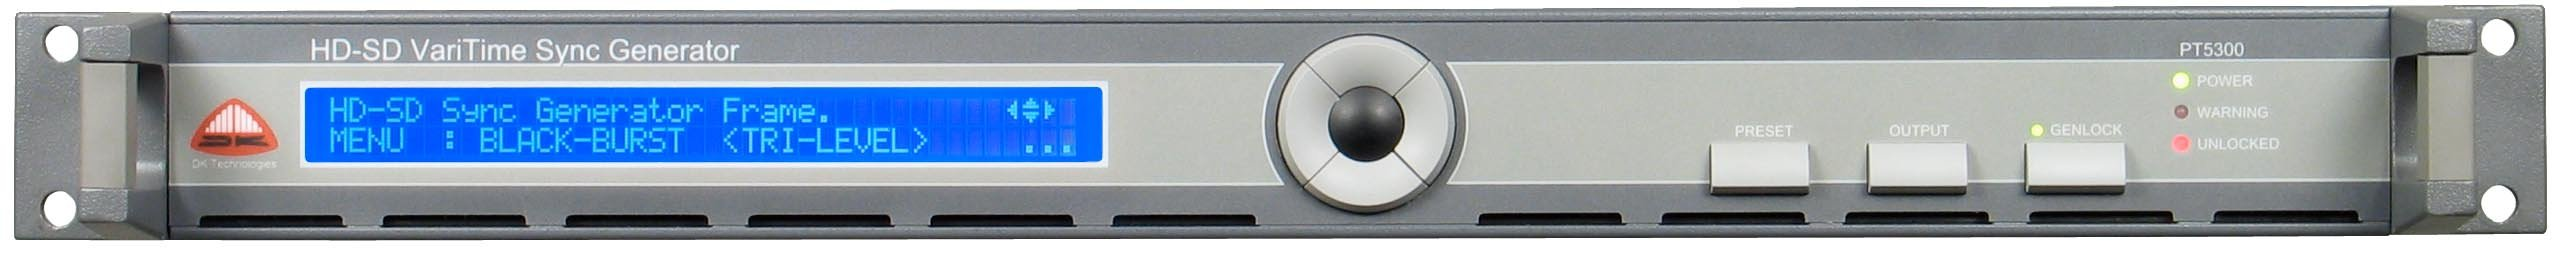
\includegraphics[scale=0.18]{fig/PT5300_front}
\end{center}


\vfill
\fbox{
\parbox{0.4\textwidth}{
\textbf{Default Network Login.}\\\ttfamily Username: \DefaultUser\\Password: \DefaultPass\\\textbf{\textit{\rmfamily\tiny Username and password is case sensitive.}}
}}
%
%\begin{flushright}  
%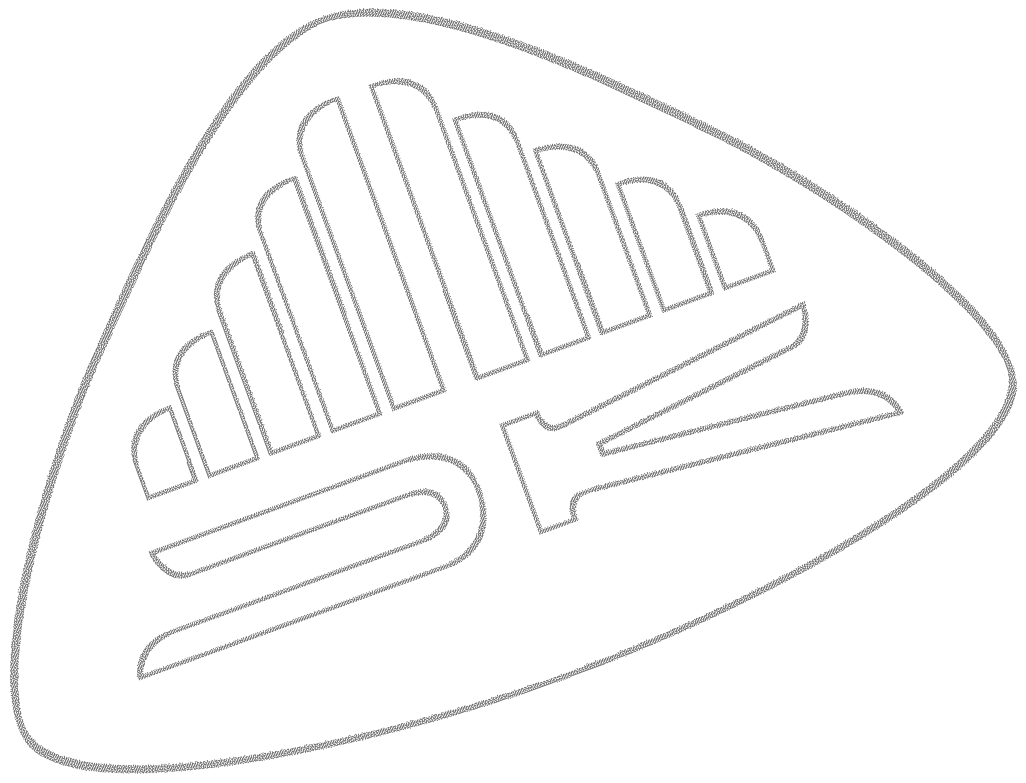
\includegraphics[scale=2]{fig/DK-Logo_gray}
%\end{flushright}
%\vfill 
%\spectabular
%\fbox{\parbox{0.4\textwidth}{\textbf{Default Network Login.}\\\ttfamily Username: \DefaultUser\\Password: \DefaultPass\\\textbf{\textit{\rmfamily\tiny Username and password is case sensitive.}}}} & %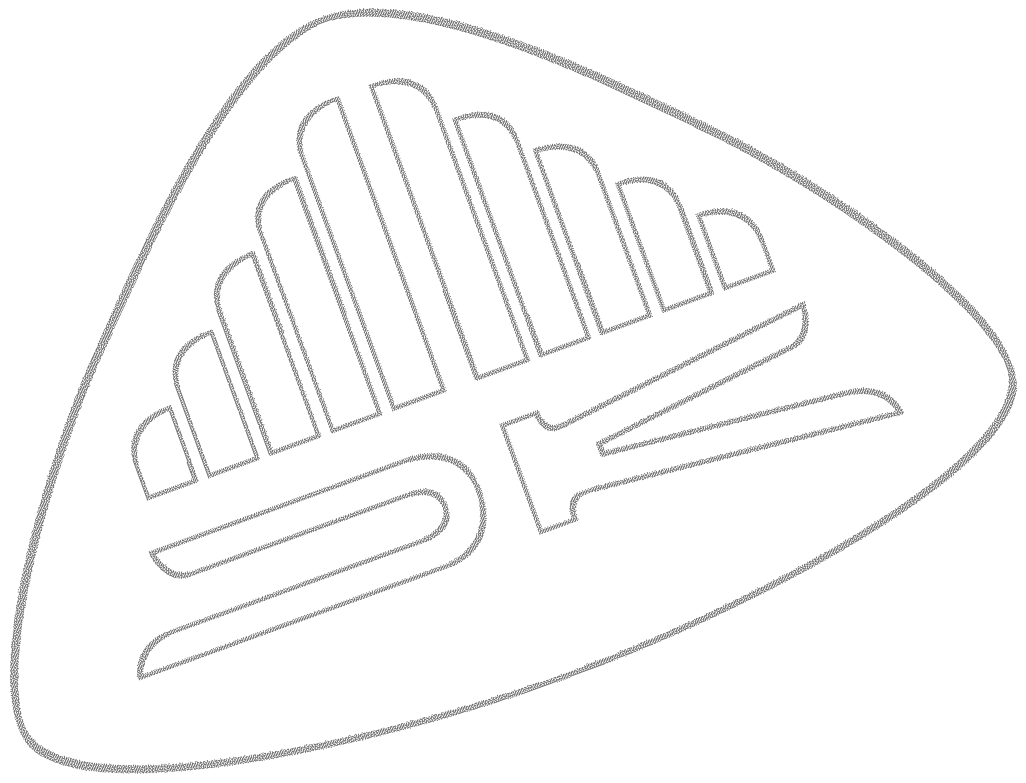
\includegraphics[scale=2]{fig/DK-Logo_gray}
%\end{tabular*}




\newpage

%%%%%%%%%%%%%%%%%%% Titelblad %%%%%%%%%%%%%%%%%%%%%
\noindent
\textbf{\Title}
\vspace{1cm}

\noindent
\textbf{Trademarks:}\\
%PT5300\texttrademark\ is a registered trademark of DK-Technologies A/S.

Windows\registeredtm is a registered trademark of Microsoft Corporation, One Microsoft Way, Redmond, Washington 98052-6399 U.S.A.
\vfill	% "fills" page with linebreaks
%
\noindent\textbf{Copyright \copyright\ 2010 \Firma}
\begin{figure}[b] \tiny\small
\begin{tabular}{ll}
\multirow{7}{*}{
\includegraphics[width=80pt]{fig/dk_logo_centreret}}	& \Firma \\
& Marielundvej 37D				  \\ 
& DK-2730 Herlev - Denmark  \\
& 												  \\
& Phone:  (+45) 44 85 02 55 \\
& Fax:    (+45) 44 85 02 50 \\
& www.dk-technologies.com - info@dk-technologies.com\\
\end{tabular}
\end{figure}

\cleardoublepage


\tableofcontents
\clearpage

\pagenumbering{arabic}	% use arabic numerals for rest of document
\pagestyle{fancy}				% switch to fancy pagestyle for headers and footers

\section{Safety}
\label{cha:Safety}

\textbf{Read this chapter carefully before installation and use of the instrument.}

\subsection{Introduction}
Adjustment, maintenance and repair of the exposed equipment shall be carried out only by qualified personnel who are aware of hazards involved.

\subsection{Safety Precautions}
For the correct and safe use of the instrument, it is essential that both operating and servicing personnel follow generally accepted safety procedures in addition to the safety precautions specified in this manual. Specific warning and caution statements, where applicable, are found throughout this manual. Note that warning and caution statements and/or symbols are marked on the instrument as well. This manual provides technical information important for safe operation of the equipment. Please refer to the relevant sections of the manual for technical specifications, installation and
operating instructions. 

Special attention must be paid to the following issues:

\begin{itemize}
\item[-] Protective earthing of the instrument is required for the accessible terminals to be safe. (IEC 1010-1 Safety class I instrument)
%
\item[-] The actual environmental conditions must be checked against the specification.
\item[-] Mains voltage must be inside the specified range.
\end{itemize}

\subsection{Use of Caution and Warning Statements}

\paragraph{Caution}

Used to indicate correct operation or maintenance in order to prevent damage to, or destruction of equipment or other property.

\paragraph{Warning}

Used to indicate a potential hazard that requires correct procedures or practices in order to prevent personal injury.

\subsection{Symbols}
\begin{tabular}{l|l}
	\hline
	\textbf{Symbol:} & \textbf{Explanation:} \\
	\hline
	& \\
	
\includegraphics[width=2em]{fig/hazard} & Caution, risk of electric shock\\
	
\includegraphics[width=2em]{fig/caution} & Caution (refer to accompanying documents)\\
	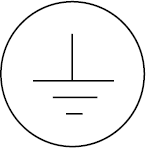
\includegraphics[width=2em]{fig/ground_symbol} & Protective conductor terminal\\
	
\includegraphics[width=2em]{fig/AC_symbol} & Alternating current\\
%	\multirow{3}{*}{
\includegraphics[width=2em]{fig/on_off_switch}} 	& Off (supply - mains switch)\\
%																																		&														\\
%																																		& On (supply - mains switch)\\
\end{tabular}

\subsection{Impaired Safety Protection}

Whenever it is likely that safe operation is impaired, the instrument must be made inoperative and secured against unintended operation. The appropriate servicing authority must be informed. For example, safety is likely to be impaired if the instrument fails to perform the intended functions or shows visible damage.

\begin{center}
\fbox{
\parbox{0.95\textwidth}{
\textbf{WARNING}: Protection provided by the equipment may be impaired, if the equipment is used in a manner not specified by this manual.
}}
\end{center}

\subsection{Technical Assistance}
Technical assistance may be obtained from your local DK-Technologies customer support organization or from:

\begin{tabular}{@{}l}
{\large DK-Technologies A/S }\\
Marielundvej 37D\\
DK-2730 Herlev\\
Denmark\\
\end{tabular}

\begin{tabular}{@{}l l}
Phone: & +45 4485 0255\\
Fax: & +45 4485 0250\\
E-Mail: & info@dk-technologies.com\\
Website: & \href{http://www.dk-technologies.com}{http://www.dk-technologies.com/}\\
\end{tabular}
\clearpage
\section{Introduction and Applications}
\label{cha:Introduction and Applications}
\subsection{Introduction}
The PT 5300 HD-SD Varitime\TM Sync Generator is specially designed to fit into HD as well as SD digital and mixed digital/analogue video installations, and it provides signals for synchronisation, fault finding and checking of the entire digital chain. Because of its many parallel outputs, the PT 5300 is ideal for supplying the video switcher with all commonly used test signals for alignment, but also as a stand-by pattern source.

The basic generator is available as a SD or HD-SD gen-lockable sync / test signal generator with 2 Black Burst outputs. In the HD-SD version it has furthermore 4 Tri-Level sync outputs available. 

Several generators can be added to the basic unit, making up to 4 different HD or SD SDI signals available at a time. Instead of SDI generators, one or two analogue test pattern generator modules can be added.

All HD-SD SDI generators are switchable between 625 and 525 lines and the various HD formats, but differ in the number of signals, embedded audio, and other features. The analogue composite generator is a dual standard, PAL and NTSC, and provides test signals and the PTV pattern.

Except for the basic SDI generator, all HD-SD SDI generators and the analogue test pattern generator can superimpose three lines of text on the video signals. With complex test patterns, the text is automatically placed in the black text fields.

Other available options are:
\begin{itemize}
	\item[-] Dual link HD-SD Test signal generator
	\item[-] AES/EBU digital audio generator
	\item[-] Digital genlock
	\item[-] Time clock interface
\end{itemize}

The PT 5300 is gen-lockable to a traditional Black Burst signal, but can also be locked onto a continuous wave. It can even lock onto a 525-line video signal and still generate PAL, 625-line SD-SDI signals and HD SDI signals in the major parts of formats.

Each of the outputs can be individually timed: SD-SDI signals can be timed in steps of 37 ns over a ${\pm}$1 field range; HD-SDI and Tri-Level Sync signals in steps of 6.7 ns, the analogue Black Bursts and test pattern outputs are timeable in steps of 0.5\degrees of subcarrier over a ${\pm}$4 field sequence for PAL and ${\pm}$2 field sequence for NTSC.

The stability of the internal reference oscillator ensures accurate signals when the PT 5300 is acting as a reference generator.

It is not unusual for a Philips stand-by pattern to display the time and date as well; an optional module interfaces with LTC, VITC, or the internal video reference.

AES/EBU digital audio is available on both XLR and BNC connectors. The generator module has two built-in generators, which can be programmed independently with silence or with tones that include signals with audible left/right indication. The AES/EBU output signals are always locked both to the 525-line and 625-line outputs. In multistandard operation, this permits direct connection between AES/EBU generators in 525-line and 625-line environments. A separate word-clock signal is available on a BNC connector.

\subsection{Applications}
The PT 5300 can be used in a multitude of different applications, e.g. delivering signals for a video switcher, as a master and as backup Sync Pulse Generator(SPG) and as a general video signal generator. 

In small studios and in OB-vans it can both work as an SPG while also delivering test signals at the same time. It also operates in backup configurations to a PT 5210 Varitime\TM Digital Sync Generator and a PT 5211 Varitime\TM Changeover Unit. Built-in fault detection circuitry determines when to send an error flag to the Changeover unit.

One of the SDI test signal generator options supplies all ITU801-specified test signals, as well as other signals. This enables a complete test of the digital video lines and the conversion process to the analogue domain.

In digital distribution networks where data compression is used, a stationary test signal will not reveal if the line is in a ``freeze'' mode. A moving bar added to the standby pattern will show if the line is open and if the time and date appears in the pattern, this is a good indication that the line is not frozen.

The time information can be locked onto either VITC, LTC, or the internal video reference. The time can be offset to cope with delays in distribution, MPEG-2 coding and transmission. It also ensures that the ``true'' time can be displayed at the reception point.

Serial digital genlock is used in remote installations where distribution of the master sync takes place via optical fibre. This facility is available in the SDI gen-lock option, PT8606.

Six complete instrument presets have been included to enable quick changes in operation mode. Each of the set-up may be given names with a string of up to a 16 character.

In automated applications, the RS 232 remote control interface provides full control over all functions of the generator. Parameters for each output can be adjusted remotely and a complete set-up can be transmitted to and from the instrument.

In addition, the RS 232 interface can be exchanged with a simple ground closure control with a selection of presets and a few basic functions.

\clearpage
\section{Product Data}
\label{cha:Product Data}

\subsection{Safety Characteristics}
This apparatus has been designed and tested in accordance with the safety Class I requirements of the IEC publication 1010-1 (``Safety Requirements for Electrical Measuring Apparatus''), and is safe as supplied. This manual contains information and warnings, which must be followed during operation to ensure operator and service personnel safety.

\subsection{Performance Characteristics}
Characteristics expressed in numerical values with stated tolerances are guaranteed tolerances, when the instrument is calibrated at 20-30\degrees C and after 20 min. warm-up. Specified non-tolerance numerical data indicate typical values at nominal ambient temperature (25\degrees C) and reflects an average performance.

\subsection{Versions}
The generator is based on two basic versions, one for SD-SDI and analogue applications and one for HD-SD SDI and analogue applications. The HD SD version includes the Tri-level Sync option (PT 8611). Both versions are gen-lockable sync pulse generators with further 2 x Black Burst outputs as well. To the basic configuration a number of units can be added. 

The apparatus is a multiformat, simultaneously covering SD-SDI (625/525), analogue PAL and analogue NTSC and the extended version with additional HD Tri-level sync outputs as well as HD-SDI test signal outputs. A Dual Link HD-SD-SDI generator is also available.

Additional modules covering an AES/EBU Audio generator, Digital Gen-lock input and a Time clock Interface.

All SD-SDI generators work both in 625 and 525 lines, and can be chosen between different complexities:
\begin{itemize}
\item The standard TSG (PT8603) contains all test signals, i.e. Colourbar, PLUGE, crosshatch needed in standard SPG setup where some test signals are required.
\item The Basic TSG (PT8639) contains less complex test signals, i.e. Colourbar, PLUGE, crosshatch, etc.
\item The Extended Test Pattern Generator (PT 8632) has a broad range of test signals plus one complex test pattern: PTV pattern in 625-lines, 4:3 format (separate version with FuBK pattern).
\item The high-end Test Pattern Generator (PT 8633) contains a very wide range of signals, such as PTV and FuBK test patterns in both 4:3 and 16:9 aspect ratio as well as other multistandard complex test patterns.
\end{itemize}

All HD SD-SDI generators work in 16 different HD formats plus the SD-SDI formats 625 and 525 lines, where the Tri-Level sync option (PT8611) work with 19 different HD formats.

\subsection{Options}
\begin{tabular}{l l}
	PT8603 & SDI Test Signal Generator\\
	PT8604 & Multiple Parallel Black Burst, 6 Outputs\\
	PT8606 & SD-SDI Digial Genlock\\
	PT8508 & Dual Black Burst Generator\\
	PT8609 & SDI Black and Colour Bar Generator\\
	PT8611 & Quad HD Tri-Level Sync Generator\\
	PT8612 & HD-SD SDI Test Signal Generator\\
	PT8613 & Dual link HD-SD Test Signal Generator\\
	PT8616 & GPS Genlock and LTC Generator\\
	PT8631 & Analogue Test Pattern Generator\\
	PT8632 & Test Pattern Generator, Extended\\
	PT8633 & SDI Test Pattern Generator, High-end\\
	PT8635 & Dual AES/EBU Digital Audio Generator\\
	PT8637 & Time Clock Interface\\
	PT8639 & SDI Test Signal Generator, Basic Signals\\
	PT8643 & Ethernet module.\\
	\rule{0pt}{4ex}
	PT8552 & Slide Rail Mounting Kit\\
\end{tabular}

Note: PT8632 comes in two versions:
\begin{itemize}
	\item PT8632/00 with Philips test pattern
	\item PT8632/10 with FuBK test pattern
\end{itemize}

\subsection{Basic Instrument}
\subsubsection{Master Frequency Reference}
\spectabular
\textbf{27 MHz master frequency:}			& Better than 0.25 ppm (0-50\degrees C, ref. 25\degrees C) \\
\textbf{Ageing:}											& $<$ 0.1 ppm/month
\end{tabular*}

\subsubsection{Analogue Genlock}
\spectabular
\textbf{Input:}						& 75 \ohm  looped through or two 75 \ohm  terminated inputs (menu configurable) \\
\textbf{Return loss:}			& $>$ 38 dB to 6 MHz
\end{tabular*}

\subsubsection{Genlock Signal (M-NTSC or G-PAL)}
\spectabular
\textbf{Amplitude:} 					& Nominally $\pm$ 3 dB \\
\textbf{S/N ration:} 					& $>$ 26 dB \\
\textbf{Sc-H phase:} 					& Nominally $\pm$ 45\degrees \\
\textbf{Pull-in range fsc:} 	& $\pm$ 20 Hz \\
Jitter when locked to burst:	& $<$ 0.5\degrees \\
Jitter when locked to sync: 	& $<$ 2 ns \\
\textbf{Timing range:} 				& PAL: $\pm$ 4 fields \\
															& NTSC: $\pm$ 2 fields \\
\textbf{Timing resolution:} 	& 0.5\degrees fsc \\
\end{tabular*}

\subsubsection{Genlock Signal}
\spectabular
\textbf{Continuous frequency reference:}		& Subcarrier, 5 or 10 MHz \\
\textbf{Amplitude:}													& 1 V $\pm$ 3 dB
\end{tabular*}

\subsubsection{Analogue Genlock Transparent Channel}
The analogue genlock signal is transferred via an AC-coupled amplifier to a transparent output.

\spectabular
\textbf{Output impedance:}		& 75 \ohm \\
\textbf{Return loss:}					& $>$ 36 dB to 6 MHz
\end{tabular*}

\subsubsection{Analogue Black Burst Outputs}
\spectabular
\textbf{Number of outputs:}				& 2, independently timeable \\
\textbf{Connector:}								& BNC \\
\textbf{Return loss:}							& 75 \ohm  $\pm$ 0.5 \ohm \\
\textbf{Sync Amplitude:}					& PAL: -300 mV $\pm$ 2\% \\
																	& NTSC: -286 mV $\pm$ 2\% \\
\textbf{Burst Amplitude:}					& PAL: -300 mV $\pm$ 2\% \\
																	& NTSC: -286 mV $\pm$ 2\% \\
\textbf{Timing range:}						& PAL: $\pm$ 4 fields \\
																	& PAL: $\pm$ 2 fields \\
\textbf{Timing resolution:}				& 0.5\degrees fsc \\
\textbf{Sc-H phase:}							& Default 0\degrees, adjustment $\pm$ 180\degrees, resolution $<$ 1\degrees${^{^{\circ}}}$ \\
\textbf{S/N ratio:}								& 60 dB unweighted to 5 MHz\\
\textbf{Jitter:}									& Burst jitter:	$\pm$ 0.5\degrees \\
																	& Sync jitter: $\pm$ 0.5 ns (based on design and burst jitter value) \\
\textbf{Output monitoring:} 			& Continuous of output level with error flag on ``Changeover'' connector. Detectors can be disabled
\end{tabular*}

\subsection{Communication interface}
The PT5300 is equipped with a 9 pole male D-Sub connector which provides RS232 communication to the instrument.
Please see section \ref{cha:Remote} for more information about remote control of the PT5300.

The latest version of the PT5300 is as standard also equipped with a PT8643 Ethernet module. This module provides a Telnet interface for remote control and an optional SNTP v4 Time Server. The SNTP option requires that a PT8616 GPS genlock module is installed.

\PasswordWarning

If both the computer and the PT5300 is configured with a static IP address (and the same Subnet Mask) a straight-trhough or crossover Ethernet cable can be used to connect the computer and the PT5300 directly.
%\subsection{Fast Setup}
%Readout of the entire instrument setting is possible with a single command from the remote RS232 interface. The data read can be transferred in the same format to another unit to set up the unit, or two units can be directly connected and the setting copied from one unit to the other.

\subsection{Changeover Control}
A built-in fault detection circuitry determines when to send an error flag to the PT5211 Varitime\TM Changeover Unit. Detector for each output can be disabled internally.

\subsection{Presets}
Six complete instrument preset are stored in a non-volatile memory.

The presets have names consisting of up to 16 letters. The preset name is displayed when the preset is active.

\clearpage
\subsection{Options}
\subsubsection{PT8603 SD-SDI Pattern Generator}

\begin{itemize}
	\setlength{\itemsep}{1pt}
	\setlength{\parskip}{0pt}

	\item Output Signals:
	\item[ ] Colorbar
	\item[ ] 525 line: SMPTE
	\item[ ] 625 line: EBU 75\%, ITU 75\% (8 bit), Colourbar 100\%, Split Field 75\% with gray, and Split Field 75\% with red
	\item SDI Checkfield
	\item Shallow Ramp
	\item Digital Timing Test Pattern
	\item Black
	\item Window 15\%
	\item Window 20\%
	\item Window 100\%
	\item Cross hatch
	\item PLUGE
	\item Multiburst
	\item 75\% Red
	\item Staircase signal, 5 steps
	\item Staircase signal, 10 steps
\end{itemize}

Embedded sound and EDH may be added to the test signals.
All signals are generated with 10 bit except otherwise is specified.
\clearpage
\subsubsection{PT 8604 Multiple Parallel Black Burst, 6 Outputs}
Additional 6 parallel BB outputs available are connected to the BB 2 output in the basic version
All 6 outputs having the same time plane as BB2.

\spectabular
\textbf{Connectors:} 				& 6 x BNC\\
\textbf{Output Impedance:} 	& 75 \ohm  $\pm$ 0.5 \ohm \\
\textbf{Return loss:}:			& $>$ 36 dB, up to 5 MHz\\
\textbf{Sync Amplitude:}		& 300 mV $\pm$ 2\%, (PAL), 286 mV $\pm$ 2\%, (NTSC)\\
\textbf{Burst Amplitude:}		& 300 mV $\pm$ 2\%, (PAL), 286 mV $\pm$ 2\%, (NTSC)\\
\textbf{Timing:}						& Equal to BB2 output, max. Delay 50 ns\\
\textbf{Sc-H phase:}				& Equal to BB2 output\\
\textbf{S/N ratio:}					& Better than 60 dB unweighted to 5 MHz\\
\textbf{Jitter:}						& $<$ 0.5 ns
\end{tabular*}
\clearpage
\subsubsection{PT8606 SD-SDI Digital Genlock}
SDI digital gen-lock module with active loop-through, 1 input.

\spectabular
\textbf{Connectors:}						& 2 x BNC\\
\textbf{Input/Output Impedance:}& 75 \ohm \\
\textbf{Format:}								& 270MB/s component\\
\end{tabular*}

Complies with SMPTE 259M and ITU-R BT.656
\clearpage
\subsubsection{PT8608 Dual Black Burst Generator}
2 Black Burst generators individually configurable to PAL or NTSC

\spectabular
\textbf{Number of outputs:} & 2 with independent timeable outputs\\
\textbf{Connectors:}			 	& 2 x BNC\\
\textbf{Output Impedance:} 	& 75 \ohm$ \pm$ 0.5 \ohm \\
\textbf{Return loss:}:			& $>$ 36 dB, up to 5 MHz\\
\textbf{Sync Amplitude:}		& 300 mV $\pm$ 2\%, (PAL), 286 mV $\pm$ 2\%, (NTSC)\\
\textbf{Burst Amplitude:}		& 300 mV $\pm$ 2\%, (PAL), 286 mV $\pm$ 2\%, (NTSC)\\
\textbf{Timing range:}			& $\pm$ 4 fields (PAL), $\pm$ 2 fields (NTSC)\\
\textbf{Timing resolution:}	& 0.5\degrees  of subcarrier\\
\textbf{Sc-H phase:}				& Default 0\degrees, adjustment $\pm$ 180\degrees, resolution $<$ 1\degrees \\
\textbf{S/N ratio:}					& Better than 60 dB unweighted to 5 MHz\\
\textbf{Jitter:}						& $< \pm$ 0.5 ns
\end{tabular*}
\clearpage
\subsubsection{PT8609 SDI Black and Colour Bar Generator}
Each board has two identical outputs

\spectabular
\textbf{Signals:} 					& SD-SDI black, EBU 75\% and 100\% colour bar (625 lines), or SMPTE colour bar (525 lines)\\
\textbf{Formats:}					 	& 270 Mb/s component, complies with ITU-R BT 656 and SMPTE 259M\\
\textbf{Data format:}				& Scrambled NRZI 270Mb/s\\
\textbf{Connectors:}			 	& 2 x BNC\\
\textbf{Output Impedance:} 	& 75 \ohm \\
\textbf{Return loss:}:			& $>$ 15 dB, 5 to 270 MHz\\
\textbf{Amplitude:}					& 800 mV $\pm$ 10\% \\
\textbf{Jitter:}						& $<$ 0.2 UI\\
\textbf{Timing range:}			& $\pm$ 1 field\\
\textbf{Timing resolution:}	& 37.5 ns (one half cycle of the 13.5 MHz clock)\\
\textbf{Embedded Audio:}		& Silence on/off \\
\textbf{Ancillery data:}		& EDH: on/off\\
 														& Ancillary data on/off\\

\end{tabular*}
\clearpage
\subsubsection{PT8611 Quad HD Tri-Level Sync Generator}
4 generators individually configurable to 20 HD Tri-Level Sync formats

\spectabular
\textbf{Number of outputs:}			& 4 with independent timeable outputs\\
\textbf{HD Formats:}						& 720p, 1080i, 1080p. Frame rates as listed in table \ref{tab:8611formats}
\end{tabular*}

\begin{table}[hbt]
\centering
\begin{tabular}{|l|c|c|p{0.5em}|}
\cline{1-3}
Format 1)			& PT 8611 Tri-Level Sync	& Gen-lock to BB/SDI  \\
\cline{1-3}
\hline
1080p/60			& x	& 	& \multirow{8}{*}{\begin{sideways}{\tiny HD 1080p}\end{sideways}} \\
\cline{1-3}
1080p/59.94		& x	&		& \\
\cline{1-3}
1080p/50			&	x	&		& \\
\cline{1-3}
1080p/30			&	x	&		& \\
\cline{1-3}
1080p/29.97		&	x	&	x	& \\
\cline{1-3}
1080p/25			&	x	&	x	& \\
\cline{1-3}
1080p/24			&	x	&		& \\
\cline{1-3}
1080p/23.98		&	x	&		& \\
\hline
\hline
1080i/30			& x	& 	& \multirow{3}{*}{\begin{sideways}{\tiny HD 1080i}\end{sideways}} \\
\cline{1-3}
1080i/29.97 	& x & x & \\
\cline{1-3}
1080i/25 			& x & x & \\
\hline
\hline
1080sF/30			& x	& 	& \multirow{5}{*}{\begin{sideways}{\tiny HD 1080sF}\end{sideways}} \\
\cline{1-3}
1080sF/29.97	&	x	&	x	& \\
\cline{1-3}
1080sF/25			&	x	&	x	& \\
\cline{1-3}
1080sF/24			&	x	&		& \\
\cline{1-3}
1080sF/23.98	&	x	&		& \\
\hline
\hline
720p/60				& x	& 	& \multirow{8}{*}{\begin{sideways}{\tiny HD 720p}\end{sideways}} \\
\cline{1-3}
720p/59.94		& x	&	x	& \\
\cline{1-3}
720p/50				&	x	&	x	& \\
\cline{1-3}
720p/30				&	x	&		& \\
\cline{1-3}
720p/29.97		&	x	&	x	& \\
\cline{1-3}
720p/25				&	x	&	x	& \\
\cline{1-3}
720p/24				&	x	&		& \\
\cline{1-3}
720p/23.98		&	x	&		& \\
\hline
\hline
576i/25 (625)			& 	& x	& \multirow{2}{*}{\begin{sideways}{\tiny SD}\end{sideways}} \\
\cline{1-3}
487i/29.97 (525)	&		&	x	& \\
\hline
\end{tabular}
\caption{HD Tri-Level sync formats supported by PT5300HD}
\label{tab:8611formats}
\end{table}

\spectabular
\textbf{Connectors:}			 	& 4 x BNC\\
\textbf{Output Impedance:} 	& 75 \ohm \\
\textbf{Return loss:}:			& $>$ 30 dB, 5 to 30 MHz\\
\textbf{Amplitude:}					& 600 m\Vpp $\pm$ 2\% \\
\textbf{Jitter:}						& $<\pm$ 2\%\\

\end{tabular*}
\clearpage
\subsubsection{PT 8612 Quad HD-SD serial digital test signal Generator}
Four generators individually configurable with HD and SD test signals

\spectabular
\textbf{Number of outputs:}			& 4 with independent timeable outputs\\
\textbf{HD Formats:}						& 720p, 1080i, 1080p. Frame rates as listed in table \ref{tab:8612formats}
\end{tabular*}

\textbf{Signals:}
\begin{itemize}
\item[-] \textbf{Video:} EBU Colour Bar, 75\% with 100\% white; Colour Bar, 100\%, with 100\% white; SDIcheckfield;
PLUGE; window signals; clapper board; luminance ramp; combination pattern
with selectable colour bar - white ramp - LIP SYNC - 75\% red; Black, full field; white, full
field from -5\% to 105\% in 5\% increments; white, window from 5\% to 105\% in 5\% increments; cross hatch, 16 x 9
\item[-] \textbf{Text:} Moving text string with up to 3 lines of 16 characters each line inserted in the test signals
\item[-] \textbf{Audio:} Test-tones embedded in the HD-SD SDI signals
\end{itemize}

\begin{table}[hbt]
%\centering
\begin{tabular}{|l|c|c|p{0.5em}|}
\cline{1-3}
Format 1)			& PT 8611 Tri-Level Sync	& Gen-lock to BB/SDI  \\
\cline{1-3}
\hline
1080p/60			& x	& 	& \multirow{8}{*}{\begin{sideways}{\tiny HD 1080p}\end{sideways}} \\
\cline{1-3}
1080p/59.94		& x	&		& \\
\cline{1-3}
1080p/50			&	x	&		& \\
\cline{1-3}
1080p/30			&	x	&		& \\
\cline{1-3}
1080p/29.97		&	x	&	x	& \\
\cline{1-3}
1080p/25			&	x	&	x	& \\
\cline{1-3}
1080p/24			&	x	&		& \\
\cline{1-3}
1080p/23.98		&	x	&		& \\
\hline
\hline
1080i/30			& x	& 	& \multirow{3}{2cm}{\begin{sideways}{\tiny HD 1080i}\end{sideways}} \\
\cline{1-3}
1080i/29.97 	& x & x & \\
\cline{1-3}
1080i/25 			& x & x & \\
\hline
\hline
720p/60				& x	& 	& \multirow{8}{*}{\begin{sideways}{\tiny HD 720p}\end{sideways}} \\
\cline{1-3}
720p/59.94		& x	&	x	& \\
\cline{1-3}
720p/50				&	x	&	x	& \\
\cline{1-3}
720p/30				&	x	&		& \\
\cline{1-3}
720p/29.97		&	x	&	x	& \\
\cline{1-3}
720p/25				&	x	&	x	& \\
\cline{1-3}
720p/24				&	x	&		& \\
\cline{1-3}
720p/23.98		&	x	&		& \\
\hline
\hline
576i/25 (625)			& 	& x	& \multirow{2}{*}{\begin{sideways}{\tiny SD}\end{sideways}} \\
\cline{1-3}
487i/29.97 (525)	&		&	x	& \\
\hline
\end{tabular}
\caption{HD-SD serial digital test signals supported by PT5300HD}
\label{tab:8612formats}
\end{table}

\spectabular
\textbf{Connectors:}			 	& 4 x BNC\\
\textbf{Output Impedance:} 	& 75 \ohm $\pm$1\% \\
\textbf{Return loss:}:			& $>$ 15 dB, 5 to 1.5 GHz\\
\textbf{Amplitude:}					& 800 m\Vpp $\pm$ 2\% \\
\textbf{Jitter:}						& $<\pm$ 1/2 frame\\
\textbf{Timing resolution:} & \\
\textbf{- HD:}							& 6.7 ns \\
\textbf{- SD:}							& 6.7 ns \\
\end{tabular*}
\clearpage
\subsubsection{PT 8613 Dual link HD-SD Test Signal Generator}
Two generators individually configurable, Multiformat HD Dual link, HD Single link and SD-SDI
test generator. Dual link in 1080p, 1080i and 1080sF formats only.

\spectabular
\textbf{Number of outputs:}			& 2 generators independently timeable. Each of the two
generators have link A and link B for dual link operation \\
\textbf{HD Formats:}						& 720p, 1080i, 1080p, 1080sF. Frame rates as listed in table \ref{tab:8613formats} \\
\textbf{Video interface:}				& \\
\textbf{HD Dual Link:} 					& GBRA 4:4:4:4 12-bit \\
																& GBR 4:4:4 10-bit \\
																& \YCBCR 4:4:4:4 12-bit\\
																& \YCBCR 4:4:4 10-bit\\
																& \YCBCR 4:2:2:4 12-bit \\
\textbf{Single Link:}						& HD; \YCBCR 4:2:2 10-bit\\
																& SD; \YCBCR 10-bit.
\end{tabular*}

\textbf{Signals:}
\begin{itemize}
\item \textbf{Dual Link Video:} EBU Colour Bar, 75\% with 100\% white; Colour Bar, 100\%, with 100\% white; SDI- checkfield; PLUGE; window signals; clapper board; luminance ramp; combination pattern with selectable colour bar - white ramp - LIP SYNC - 75\% red; Black, full field; white, full field from -5\% to 105\% in 5\% increments; white, window from 5\% to 105\% in 5\% increments; cross hatch, 16 x 9
\item \textbf{Single Link Video:} same signals and same timing as mentioned above but output B is just
black video
\item \textbf{Text:} Moving text string with up to 3 lines of 16 characters each line inserted in the test signals. The font size can be changed as well as the font colour and the background colour. The position of the text can be in a fixed pos. and/or it can be moved horizontally and vertically
\item \textbf{Audio:} 16 channels of audio can be embedded into the video stream. In Dual Link operation the audio is embedded in link A
\item \textbf{Audio Signals:} Silence, Sine, Click 
\item \textbf{Audio Levels:} 0dBFS, -6dBFS,-12dBFS, -18dBFS, -20dBFS, -24DBFS
\item \textbf{Lip Sync timing:} $\pm$ 500 ms relative to video, adjustable
\end{itemize}

\begin{table}[hbt]
%\centering
\begin{tabular}{|l|c|c|p{0.5em}|}
\cline{1-3}
Format 1)			& PT 8613 TSG	& Gen-lock to BB/SDI \\
\cline{1-3}
\hline
1080p/60			&  	& 	& \multirow{8}{*}{\begin{sideways}{\tiny HD 1080p}\end{sideways}} \\
\cline{1-3}
1080p/59.94		&  	&		& \\
\cline{1-3}
1080p/50			&	 	&		& \\
\cline{1-3}
1080p/30			&	x	&		& \\
\cline{1-3}
1080p/29.97		&	x	&	x	& \\
\cline{1-3}
1080p/25			&	x	&	x	& \\
\cline{1-3}
1080p/24			&	x	&		& \\
\cline{1-3}
1080p/23.98		&	x	&		& \\
\hline
\hline
1080i/30			& x	& 	& \multirow{3}{2cm}{\begin{sideways}{\tiny HD 1080i}\end{sideways}} \\
\cline{1-3}
1080i/29.97 	& x & x & \\
\cline{1-3}
1080i/25 			& x & x & \\
\hline
\hline
1080sF/30			& x	& 	& \multirow{5}{2cm}{\begin{sideways}{\tiny HD 1080sF}\end{sideways}} \\
\cline{1-3}
1080sF/29.97	&	x	&	x	& \\
\cline{1-3}
1080sF/25			&	x	&	x	& \\
\cline{1-3}
1080sF/24			&	x	&		& \\
\cline{1-3}
1080sF/23.98	&	x	&		& \\
\hline
\hline
720p/60				& x	& 	& \multirow{8}{*}{\begin{sideways}{\tiny HD 720p}\end{sideways}} \\
\cline{1-3}
720p/59.94		& x	&	x	& \\
\cline{1-3}
720p/50				&	x	&	x	& \\
\cline{1-3}
720p/30				&	x	&		& \\
\cline{1-3}
720p/29.97		&	x	&	x	& \\
\cline{1-3}
720p/25				&	x	&	x	& \\
\cline{1-3}
720p/24				&	x	&		& \\
\cline{1-3}
720p/23.98		&	x	&		& \\
\hline
\hline
576i/25 (625)			& x	& x	& \multirow{2}{*}{\begin{sideways}{\tiny SD}\end{sideways}} \\
\cline{1-3}
487i/29.97 (525)	&	x	&	x	& \\
\hline
\end{tabular}
\caption{HD dual / single and SD serial digital test signals supported by PT5300HD}
\label{tab:8613formats}
\end{table}

\spectabular
\textbf{Connectors:}			 	& 4 x BNC\\
\textbf{Output Impedance:} 	& 75 \ohm $\pm$1\% \\
\textbf{Return loss:}:			& $>$ 15 dB, 5 to 1.5 GHz\\
\textbf{Amplitude:}					& 800 m\Vpp $\pm$ 2\% \\
\textbf{Jitter:}						& $<\pm$ 1/2 frame\\
\textbf{Timing resolution:} & \\
\textbf{- HD:}							& 6.7 ns \\
\textbf{- SD:}							& 6.7 ns \\
\end{tabular*}

\textbf{Embedded audio:}
16 channels of audio can be embedded into one video stream. In dual link operation the audio
is embedded in link A.

\spectabular
\textbf{Audio Signals:}			 	& Silence, Sine wave, click\\
\textbf{Audio Levels:}				& 0 dBFS, -6 dBFS, -12 dBFS, -18 dBFS, -24 dBFS \\
\textbf{Lip sync timing:}			& $\pm$ 500 ms relative to video \\
\end{tabular*}


\clearpage
\subsubsection{PT 8616 GPS Genlock and LTC Generator}

\textbf{GPS active antenna input:}\\
\spectabular
\textbf{Connectors:}											& BNC\\
\textbf{Input Impedance:}									& 50 \ohm \\
\textbf{Active amplifier supply voltage:}	& 3.3 V\\
Max power consumption:										& 0.165 W \\
\end{tabular*}

\textbf{LTC outputs:}\\
\spectabular
\textbf{Connectors:}											& 1 x XLR, balanced output, 110 \ohm \\
(Alternative)															& 2 x BNC, balanced output, 50 \ohm \\
\textbf{Output voltage:}									& 1 \Vpp \\
\textbf{Timing:}													& $\pm$ 500 ms\\
\textbf{Step size:}												& 6.7 ns\\
\end{tabular*}

\textbf{Stability:}\\
\spectabular
\textbf{Accuracy:}												& 15 ns \\
\textbf{Absolute long term drift:}				& $>$ 15 \us \\
\textbf{Absolute short term drift:}				& $>$ 1 \us \\
\end{tabular*}

\textbf{Supported LTC formats:}\\
\begin{tabular}{l}
625 lines, 25 FPS, (PAL) \\
525 lines, 29.97 FPS, (NTSC - dropframe) \\
525 lines, 29.97 FPS, (NTSC - non dropframe) \\
30 FPS \\
24 FPS \\
\end{tabular}

\textbf{Standard boot up time, (depending on sky view)} \\
\spectabular
\textbf{Cold start:}												& 44 s \\
\textbf{Warm start:}												& 18 s \\
\end{tabular*}

\textbf{Included features:}\\
\spectabular
\multicolumn{2}{l}{Selectable switching for daylight saving time:} \\

	
																												& 1: None \\
																												& 2: Confirm \\
																												& 3: Auto \\
\multicolumn{2}{l}{Individual timing offset for both LTC outputs:} \\
																												& $\pm$ 500 ms offset range \\
\end{tabular*}
\clearpage
\subsubsection{PT8631 Analogue Test Pattern Generator}

\spectabular
\textbf{Connectors:}								& 2 x BNC\\
\textbf{Output Impedance:}					& 75 \ohm  $\pm$ 0.5 \ohm\\
\textbf{Return loss:}								& $>$ 36 dB, up to 5 MHz\\
\textbf{Sync amplitude:}						& PAL: -300 mV $\pm$ 2\% \\
																		& NTSC: -286 mV $\pm$ 2\% (40 IRE$\pm$ 1 IRE) \\
\textbf{Video amplitude:}						& PAL: 700 mV $\pm$ 1\% \\
																		& NTSC: 714 mV $\pm$ 1\% (100 IRE$\pm$ 1 IRE) \\
\textbf{Burst amplitude:}						& PAL: 300 mV $\pm$ 2\% \\
																		& NTSC: 286 mV $\pm$ 2\% (40 IRE$\pm$ 1 IRE) \\
\textbf{Timing range:}							& PAL: $\pm$ 4 fields \\
																		& NTSC $\pm$ 2 fields \\
\textbf{Timing resolution:}					& 0.5\degrees  at f\footnotesize{\raisebox{-0.7ex}{SC}} \\
\textbf{Sc-H phase:}								& Default 0\degrees, adjustment $\pm$ 180\degrees, resolution $<$1\degrees \\
\textbf{PAL colour ID:}							& Line 7 field 1 (selectable ON/OFF) \\
\textbf{S/N ratio:}									& 60 dB unweighted to 5 MHz \\
\textbf{Burst Jitter:}							& $\pm$ 0.5\degrees \\
\textbf{Sync jitter:}								& 0.5 ns (based on design and burst jitter value) \\
\textbf{Frequency response:}				& $\pm$ 1\% up to 5 MHz \\
\textbf{Group delay:}								& $<$ 10 ns up to 5 MHz \\
\textbf{Chrominance / Luminance delay:}	& $<$ 5 ns \\
\textbf{Static non-linearity:}			& $<$ 1\%, typically 0.5\% \\
\textbf{Diff. Gain:}								& $<$ 0.6\%, typically 0.2\% \\
\textbf{Diff. Phase:}								& $<$ 0.6\degrees, typically 0.2\degrees \\
\end{tabular*}

\textbf{Output signals:}

%\begin{multicols}{2}{

\begin{itemize}

\setlength{\itemsep}{1pt}
\setlength{\parskip}{0pt}

\item Colourbars

\item \textbf{525-lines NTSC:}
\begin{itemize}
\item SMPTE bar
\item FCC Colourbar
\item Red 75\%
\end{itemize}

\item \textbf{625-lins PAL:}
\begin{itemize}
\item EBU bar
\item 100\% bar
\item 75\% bar with grey
\item 75\% bar with red
\item Red, 75\%
\end{itemize}

\item Multiburst
\item Luminance sweep
\item Multipulse
\item Sinx/x
\item Test lines:
\begin{itemize}
\item \textbf{PAL:}
\item CCIR18
\item CCIR17
\item CCIR330
\item CCIR331
\item \textbf{NTSC:}
\item NTC-7 Combination
\item NTC-7 Composite
\item FCC Multiburst
\item FCC Composite
\end{itemize}

\item 15\% window
\item 20\% window
\item 100\% window
\item 50\% flat field
\item 100\% flat field
\item black
\item Field squarewave
\item Alternating Black/White, 0.1 Hz
\item Luminance ramp
\item Modulated ramp
\item Staircase, 5 steps
\item Modulated staircase, 5 steps
\item Staircase, 10 steps
\item Pulse and bar
\item Crosshatch, 4:3 and 16:9 format
\item PLUGE
\item Safe area
\item VMT01 test pattern (only 625 lines)
\item Circle on black background, 4:3 aspect ratio
\item Circle on black background, 16:9 aspect ratio
\item VMT01 test pattern (only 625 lines)
\item Circle on black background, 4:3 aspect ratio
\item Circle on black background, 16:9 aspect ratio
\item Philips test pattern:
\begin{itemize}
\item 625 lines in 4:3 aspect ratio
\item 625 lines in 16:9 aspect ratio
\item 525 lines in 4:3 aspect ratio
\item 525 lines in 16:9 aspect ratio
\end{itemize}
\item FuBK test pattern:
\begin{itemize}
\item 625 lines in 4:3 aspect ratio
\item 625 lines in 16:9 aspect ratio
\end{itemize}
\end{itemize}

%}
%\end{multicols}

\textbf{Note:} The Philips test pattern can be configured in respect to:
\begin{itemize}
\item 5/10 step staircase
\item Anti-PAL ON/OFF
\item PLUGE ON/OFF
\end{itemize}

%\textit{For detailed signal descriptions, please refer to Appendix XXX}

\paragraph{Source Identification:}
\spectabular
Standard signals:			& Three strings with up to 16 characters can be added to the signal \\
Philips Test Pattern:	& Text in upper and lower text area. Time and date inserted in centre part of crosshatch lines \\
\end{tabular*}

\paragraph{Output monitoring}
Continuous of output level with error flag on ``Change-over'' connector. Detector can be disabled.


\clearpage
\subsubsection{PT8632 SDI Test pattern Generator, Extended}

\spectabular
\textbf{Connectors:}								& 2 x BNC\\
\textbf{Format:}										& 270 Mb/s component \\
																		& Complies with ITU-R BT 656 and SMPTE 259M \\
\textbf{Data format:}								& Scrambled NRZI 270 Mbit/s \\
\textbf{Output Impedance:}					& 75 \ohm \\
\textbf{Return loss:}								& $>$ 15 dB, 5 to 270 MHz\\
\textbf{Amplitude:}									& 800 mV $\pm$ 10\% \\
\textbf{Jitter:}										& $<$0.2 UI (one UI equals 3.7 ns) \\
\textbf{Timing range:}							& 525/60: $\pm$ 1 field \\
																		& 625/50: $\pm$ 1 field \\
\textbf{Timing resolution:}					& 37.5 ns (one half clock cycle on the 13.5 MHz clock) \\
\textbf{Ancillary data:}						& \\
\textbf{EDH:}												& ON/OFF \\
\textbf{Embedded audio:}						& \\
\textbf{Position:}									& Audio group 1, channels 1-4 \\
\textbf{Output signals:}						& Stereo 800Hz, No click \\
																		& Stereo 1 kHz, No click \\
																		& Stereo EBU 1 kHz, Single click in Ch. A \\
																		& Stereo BBC 1 kHz, Single click in Ch.A and double click in Ch.B \\
																		& Mono EBU 1 kHz, Single click in both Ch. A and Ch. B \\
																		& Mono, No click \\
																		& Dual, 1 kHz in Ch. A, 400Hz in Ch. B, No Click \\
																		& Wordclock, 48 kHz \\
\textbf{Output levels:}							& Silence, 0, -9, -12, -15, -16, -18, -20 dBFS \\
\textbf{Preemphasis:}								& None \\
\end{tabular*}

\textbf{Output signals:}
\begin{itemize}

\setlength{\itemsep}{1pt}
\setlength{\parskip}{0pt}

\item Colourbar
\item \textbf{525-lines:}
\begin{itemize}
\item SMPTE bar
\item FCC Colourbar
\item 75\% Colourbar, ITU 801 (timing and levels acc. to ITU801)
\item 100\% bar
\item Red 75\%
\end{itemize}
\item \textbf{625-lines:}
\begin{itemize}
\item EBU
\item 75\% Colourbar, ITU 801 (timing and levels acc. to ITU801)
\item 100\% Bar
\item 75\% bar with grey
\item 75\% bar with red
\item Red, 75\%
\end{itemize}

\item Multiburst in Y,CR and CB
\item Luminance sweep
\item Multipulse
\item 15\% window
\item 20\% window
\item 100\% window
\item Black
\item Check Field
\item Timing Test
\item Field delay test
\item Bow-Tie
\item Digital/Analogue markers
\item Digital Grey
\item Field squarewave
\item Shallow Ramp
\item Luminance ramp
\item Limit Ramp
\item Valid Ramp
\item Staircase, 5 steps
\item Modulated staircase
\item Pulse and bar
\item Crosshatch
\item PLUGE
\item Philips test pattern: 625 lines in 4:3 aspect ratio

\end{itemize}

\textbf{Note:} The Philips test pattern can be configured in respect to:
\begin{itemize}
\item Moving bar On/Off
\item 5/10 step staircase
\item Anti-PAL On/Off
\end{itemize}

\paragraph{Version PT8632/10}
In this version of the SDI generator, the Philips test pattern has been exchanged with a FuBK
test pattern in 4:3 aspect ratio

%\textit{For detailed signal descriptions, please refer to Appendix XXX}

\paragraph{Source Identification:}
\spectabular
Standard signals:			& Three strings with up to 16 characters can be added to the signal \\
Philips Test Pattern:	& Text in upper and lower text area. Time and date inserted in centre part of crosshatch lines \\
\end{tabular*}

\paragraph{Output monitoring}
Continuous of output level with error flag on ``Change-over'' connector. Detector can be disabled.


\clearpage
\subsubsection{PT 8633 SDI Test pattern Generator, High-end}

\spectabular
\textbf{Connectors:}								& 2 x BNC\\
\textbf{Format:}										& 270 Mb/s component \\
																		& Complies with ITU-R BT 656 and SMPTE 259M \\
\textbf{Data format:}								& Scrambled NRZI 270 Mbit/s \\
\textbf{Output Impedance:}					& 75 \ohm \\
\textbf{Return loss:}								& $>$ 15 dB, 5 to 270 MHz\\
\textbf{Amplitude:}									& 800 mV $\pm$ 10\% \\
\textbf{Jitter:}										& $<$ 0.2 UI (one UI equals 3.7 ns) \\
\textbf{Timing range:}							& 525/60: $\pm$ 1 field \\
																		& 625/50: $\pm$ 1 field \\
\textbf{Timing resolution:}					& 37.5 ns (one half clock cycle on the 13.5 MHz clock) \\
\textbf{Ancillary data:}						& \\
\textbf{EDH:}												& ON/OFF \\
\textbf{Embedded audio:}						& \\
\textbf{Position:}									& Audio group 1, 2, 3 or 4 (only one group at a time), all channels in each group \\
\textbf{Output signals:}						& \\
																		& Stereo 800Hz, No click \\
																		& Stereo 1 kHz, No click \\
																		& Stereo EBU 1 kHz, Single click in Ch. A \\
																		& Stereo BBC 1 kHz, Single click in Ch.A and double click in Ch.B \\
																		& Mono EBU 1 kHz, Single click in both Ch. A and Ch. B \\
																		& Mono, No click \\
																		& Dual, 1 kHz in Ch. A, 400Hz in Ch. B, No Click \\
																		& Wordclock, 48 kHz \\
\textbf{Output levels:}							& Silence, 0, -9, -12, -15, -16, -18, -20 dBFS \\
\textbf{Preemphasis:}								& None \\
\end{tabular*}

\textbf{Output signals:}

\begin{itemize}
\setlength{\itemsep}{1pt}
\setlength{\parskip}{0pt}

\item Colourbar
\item \textbf{525-lines NTSC:}
\begin{itemize}
\item SMPTE bar
\item FCC Colourbar
\item 75\% Colourbar, ITU 801 (timing and levels acc. to ITU801) \\
\item 100\% bar \\
\item Red 75\% \\
\end{itemize}
\item \textbf{625-lins PAL:}
\begin{itemize}
\item EBU bar
\item 75\% Colourbar, ITU 801 (timing and levels acc. to ITU801) 
\item 100\% bar
\item 75\% bar with grey
\item 75\% bar with red
\item Red, 75\%
\end{itemize}

\item Multiburst in Y,C\raisebox{-0.7ex}{B} and C\raisebox{-0.7ex}{R}
\item Luminance sweep
\item Y,C\raisebox{-0.7ex}{B} and C\raisebox{-0.7ex}{R} sweep
\item Multipulse
\item 15\% window
\item 20\% window
\item 100\% window
\item Flat field 100\%
\item black
\item Check field
\item Timing test
\item Field delay test
\item Bow-Tie
\item Digital/Analogue blanking markers
\item Digital grey
\item Field squarewave
\item Alternating black/white, 0.1 Hz
\item End-of-line pulses
\item End-of-line porches (ITU801):
\begin{itemize}
\item White
\item Blue
\item Red
\item Yellow
\item Cyan
\end{itemize}
\item Shallow ramp
\item Luminance ramp (black to white)
\item Limit ramp
\item Valid ramp
\item Staircase, 5 steps
\item Modulated staircase, 5 steps
\item Staircase, 10 steps
\item Pulse and bar
\item Yellow/grey ramp
\item Grey/blue ramp
\item Cyan/grey ramp
\item Grey/red ramp
\item C\raisebox{-0.7ex}{B},Y and C\raisebox{-0.7ex}{R}, Y ramp
\item Crosshatch
\item PLUGE
\item Safe area
\item CCIR18
\item CCIR17
\item CCIR330
\item CCIR331
\item VMT01 test pattern (only 625 lines)
\item Philips test pattern:
\begin{itemize}
\item 625 lines in 4:3 aspect ratio
\item 625 lines in 16:9 aspect ratio
\item 525 lines in 4:3 aspect ratio
\item 525 lines in 16:9 aspect ratio
\end{itemize}
\item FuBK test pattern:
\begin{itemize}
\item 625 lines in 4:3 aspect ratio
\item 625 lines in 16:9 aspect ratio
\end{itemize}
\end{itemize}

\textbf{Note:} The Philips test pattern can be configured in respect to:
\begin{itemize}
\item Moving bar ON/OFF
\item 5/10 step staircase
\item Anti-PAL ON/OFF
\item PLUGE ON/OFF
\item Corner circles ON/OFF (only 16:9)
\end{itemize}

%\textit{For detailed signal descriptions, please refer to Appendix XXX}

\paragraph{Source Identification:}
\spectabular
Standard signals:					& Three strings with up to 16 characters can be added to the signal \\
Philips and FuBK Pattern:	& Philips pattern \\
													& Text in upper and lower text area. Time and date inserted in centre part of crosshatch lines \\
\end{tabular*}

\paragraph{Output monitoring}
Continuous of output level with error flag on ``Change-over'' connector. Detector can be disabled.


\clearpage
\subsubsection{PT8635 Dual AES/EBU Audio Generator}

\spectabular
\textbf{Outputs:}										& 2 x AES/EBU pairs\\
\textbf{Sampling frequency:}				& 48 KHz \\
\textbf{Data rate:}									& 3.072 MBit/s \\
\textbf{Type of outputs (Configurable)}: & \\
																		& Silence, tone or word-clock \\
\textbf{Linear coding:}							& PCM, 20 bit two's complement binary, bi-phase mark coding \\
\textbf{Single ended outputs:}			& BNC, according to AES3 ID \\
\textbf{Output Impedance:}					& 75 \ohm  $\pm$ 20\%\\
\textbf{Amplitude:}									& 1.0 V $\pm$ 10\% \\
\textbf{Rise and fall time:}				& 30-44 ns \\
\textbf{Balanced outputs:}					& XLR, according to AES3 1992 \\
\textbf{Output Impedance:}					& 110 \ohm  $\pm$ 20\%\\
\textbf{Amplitude:}									& 3\Vpp  typical \\
\textbf{Rise and fall time:}				& 10-30 ns \\
\textbf{Jitter:}										& $<$ 20 ns \\
\textbf{Wordclock output:}					& Single ended, BNC \\
\textbf{Output Impedance:}					& 75 \ohm \\
\textbf{Amplitude:}									& 2.5 \Vpp  in 75 \ohm \\

\end{tabular*}



\textbf{Output signals:}
\begin{itemize}
\setlength{\itemsep}{1pt}
\setlength{\parskip}{0pt}

\item Stereo 800Hz, No click 
\item Stereo 1 kHz, No click 
\item Stereo EBU 1 kHz, Single click in Ch. A 
\item Stereo BBC 1 kHz, Single click in Ch.A and double click in Ch.B 
\item Mono EBU 1 kHz, Single click in both Ch. A and Ch. B 
\item Mono, No click 
\item Dual, 1kHz in Ch. A, 400 Hz in Ch. B, No Click 
\item 48 KHz reference
\end{itemize}

\spectabular
\textbf{Output levels:}							& Silence, 0, -9, -12, -15, -16, -18, -20 dBFS \\
\textbf{Preemphasis:}								& None \\
\end{tabular*}

\textbf{Audio reference word clock output:}\\
48 KHz squarewave \\
\textbf{Note:} When the 110 \ohm  XLR output is used with the 48 kHz clock signal, it should be terminated by 110 \ohm  in order to obtain reliable transmission.
\clearpage
\subsubsection{PT 8637 Time Clock Interface}
\textbf{References for Time Clock:}
\begin{itemize}
\item VITC in genlock signal
\item LTC on separate XLR connector (``Time Code'')
\end{itemize}

\textbf{Programmable Time Offset:}
\begin{itemize}
\item $\pm$ 10 sec
\end{itemize}

\textbf{Priority of References:}
\begin{enumerate}
\item VITC, LTC or 1 sec. pulse
\item External/internal video reference
\item Battery backed XTAL oscillator (only when power is off)
\end{enumerate}

\paragraph{Input, VITC Code Data}
Signal is conveyed on the Gen-lock input on the Gen-lock input

\paragraph{Standard:}
\begin{tabular}{l l}
PAL:		& EBU Tech 3097E \\
NTSC:		& ANSI/SMPTE 12M 1966 \\
\end{tabular}

\paragraph{Amplitude:}
\begin{tabular}{l l}
PAL:	& 550 mV$\pm$ 5\% \\
NTSC: & 570 mV$\pm$ 5\% \\
\end{tabular}

\paragraph{Bit rate:}
\begin{tabular}{l l}
PAL:		& 1812.5 $\pm$ 0.2 kb/s \\
NTSC:		& 1789.77 $\pm$ 0.2 kb/s \\
\end{tabular}

\paragraph{Position:}
\begin{tabular}{l l}
PAL:		& Line 6-22 \\
NTSC:		& Line 10-20 \\
\end{tabular}

User bits are ignored.

\paragraph{Input, Time Code Input}
The XLR input connector is normally configured for LTC Time Code, but can be configured for a 1 second pulse input.

\paragraph{LTC code:}
\begin{tabular}{l l}
Input impedance:			& $>$ 10 Kohm \\
Input level:					& 0.8-5 \Vpp \\
\textbf{Data format:}	& User bits are ignored \\
\end{tabular}

\paragraph{Second's pulse input}
\begin{tabular}{l l}
Input impedance:			& 1 K \ohm  $\pm$10\% (50 \ohm  by internal jumper setting \\
Input level:					& 1.8-2.2 \Vpp \\
Pulse duration:				& 18 \us  - 0.4s \\
\end{tabular}


\clearpage
\subsubsection{PT8639 SDI Black and Colourbar Module}

\spectabular
\textbf{Connectors:}				& 2 x BNC	\\
\textbf{Format:}						& 270 Mb/s component \\
														& Complies with ITU-R BT 656 and SMPTE 259M \\
\textbf{Data format:} 			& Scrambled NRZI 270 Mbit/sec \\
\textbf{Output impedance:}	& 75 \ohm \\
\textbf{Return loss:} 			& $>$ 15 dB, 5 to 270 MHz \\
\textbf{Amplitude:} 				& 800 mV $\pm$ 10\% \\
\textbf{Jitter:} 						& $<$ 0.2 UI (one UI equals 3.7 ns) \\
\textbf{Timing range:}			& 525/60: $\pm$ 1 field \\
														& 625/50: $\pm$ 1 field \\
\textbf{Resolution:}				& 37.5 ns (one half clock cycle on the 13.5 MHz clock) \\
\textbf{Ancillary data:}		& \\
\textbf{EDH:} 							& ON/OFF \\
\textbf{Embedded audio:} 		& Position: audio group1, channels 1-4 \\
\textbf{Output signals:} 		& Off, Silence and 1 kHz \\
\textbf{Output levels:} 		& 0, -9, -15, -18 dBFS \\
\end{tabular*}

\textbf{Output Signal:}
\begin{itemize}
\setlength{\itemsep}{1pt}
\setlength{\parskip}{0pt}

\item Colourbars

\item \textbf{525-lines:}
\begin{itemize}
\item SMPTE bar
\item FCC
\item 75\% Colourbar, ITU 801 (timing and levels acc. to ITU801)
\item 100\% bar
\item Red 75\%
\end{itemize}

\textbf{625-lines:}
\begin{itemize}
\item EBU bar
\item 75\% Colourbar, ITU 801 (timing and levels acc. to ITU801)
\item 100\% bar
\item 75\% bar with red
\item Red, 75\%
\end{itemize}

\item Multiburst in Y,CR and CB
\item 15\% window
\item 20\% window
\item 100\% window
\item Black
\item Check field
\item Digital grey
\item Staircase, 5 step
\item Crosshatch
\item PLUGE
\end{itemize}

%\textit{For detailed signal descriptions, please refer to Appendix XXX}

\paragraph{Source identification}
None

\paragraph{Output monitoring}
Continuous of output level with error flag on ``Change-over'' connector. Detector can be disabled.
\clearpage
\subsubsection{PT8643 Ethernet Option}
\label{cha:PT8643}
The PT8643 is equipped with a IEEE 802.3 10 BASE-T Ethernet network connection. The Ethernet connection is fully compatible with 100/1000 BASE-T for both full and half duplex with auto-negotiation and automatic polarity detection and correction.



\spectabular
\textbf{Connectors:}				& 1 x RJ45 \\
														& 1 x Female 9 Pin D-SUB \\
														& 1 x Male 9 Pin D-SUB \\
\end{tabular*}

\begin{itemize}
%	\item \textbf{RS232}
%	\begin{itemize}
%		\item Serial connection using 9 pin male D-Sub for remote control of the PT5300.
%		\textbf{Baud rate:} & 300 to 9600 Baud \\
%		\textbf{Data bits:} & 7 or 8 \\
%		\textbf{Stop bits:} & 1 \\
%		\textbf{Parity:} 		& None\\
%		\textbf{Handshake:} & XON/XOFF
%	\end{itemize}
%	
%	\item \textbf{Changeover Control}
%	\begin{itemize}
%		\item Changeover control using 9 pin female D-Sub.
%		\item A built-in fault detection circuitry determines when to send an error flag to the PT5211 Varitime\TM Changeover Unit. Detector for each output can be disabled internally.
%	\end{itemize}

	\item \textbf{IPv4}
	\item \textbf{Ethernet protocols:}
	\begin{itemize}
		\item DHCP Client. \\Provides automatic configuration of IP address if a DHCP server is available in the network.
		\item Telnet Server. \\Provides remote control of the PT5300 over the network.\\Default Port: 23 (TCP)
		\item SNTP Server. (Requires an optional PT8646 GPS Genlock module.) \\Simple Network Time protocol version 4. (Unicast)\\ Port: 123 (UDP)
		\item NetFinder. \\Provides easy configuration of the PT8643 module.\\ Port: 3040 (UDP)	
	\end{itemize}
	\item \textbf{RS232 Remote control.}
	\item \textbf{Changeover control.}
\end{itemize}


\clearpage

\subsubsection{Level detectors}
All generator outputs have built-in level detectors:

\paragraph{Analogue Video Signals:}
Alarm limits $<$ -3dB or $>$ +7dB

\paragraph{SDI:}
Measures both current and voltage. When one of either is more than 2dB down, the alarm is set.

\paragraph{AES/EBU:}
Alarm limits for BNC outputs: $<$ 0.75V or $>$ 2.7V
Alarm limits for balanced outputs: $<$ 2.4V or $>$ 10V
Alarm limit for Wordclock: $<$ 1.25V

\paragraph{Response time for detection:}
Approx. 2ms.

\subsection{Mechanical and Environmental Specification}
\subsubsection{Climate Conditions}
\textbf{Ambient temperature:} 5\degrees C to 45\degrees C (41\degrees F to 113\degrees F)

\textbf{Limit range of Storage and Transportation:} -20\degrees C to 60\degrees C (-4\degrees F to 140\degrees F)

\textbf{Humidity:} Non condensing (IEC 721)

\subsubsection{Mechanical Requirements}
\paragraph{Vibration:}
Limit range for storage and transport:
30 min. in each of three directions, 10 to 150 Hz; 0.7 mmp-p and 50 m/s$^2$
max acceleration.
According to IEC-Publ. 68, test Fc.

\textbf{Note:} Unit mounted on vibration table without shock absorbing material.

\paragraph{Bump:}
Limit range for storage and transport:
1000 bumps of 100 m/s$^2$
sine, 6 ms duration in each of 3 directions.
According to IEC-Publ. 68, test Eb.

\subsubsection{Safety}
IEC1010-1

\subsubsection{Electromagnetic Compatibility:}
\begin{itemize}
\item Complying with EN 50081-1/1994 (emissions) and EN 50082-1/1992 (immunity)
\item Complying with FCC Rules \& Regulations, Part 15, Subpart J, Level B (emissions)
\end{itemize}

\subsection{Power Supply}
\begin{tabular}{l l}
Voltage: 						& 90 - 250 VAC \\
Frequency: 					& 48 - 65 Hz \\
Power consumption: 	& Maximum 90 VA with all options included \\
\end{tabular}

\subsection{Mechanical Data}
19'' rack mount cabinet

\begin{tabular}{l l}
Height:		& 44 mm (1.73'') \\
Width: 		& 483 mm (19'') \\
Depth:		& 490 mm (19.3'') \\
Weight:		& 6 kg (13.2 lbs) \\
\end{tabular}
\clearpage
\section{Accessories and Options}
\label{cha:Accessories and Options}

\subsection{Accesories}
\begin{tabular*}{\textwidth}{@{\extracolsep{\fill}}l l l}
\hline
Item: 										& Quantity: 		& Ordering Number: \\
\hline
Mains cable, EURO 				& as required 	& 4008 105 00200 \\
Mains cable, US 					& as required 	& 4008 105 00030 \\
Mains cable, UK 					& as required 	& 4008 105 01390 \\
Rubber foot selfadhesive 	& 4 						& 2822 030 90299 \\
\end{tabular*}

\subsection{Options}
\begin{tabular*}{\textwidth}{@{\extracolsep{\fill}}l l l}
\hline
Description: 							& &	Ordering Number: \\
\hline
PT 8603	& SDI Test Signal Generator 								& 9449 086 03001 \\
PT 8604	& Multiple Parallel Black Burst, 6 Outputs 	& 9449 086 04001 \\
PT 8606	& SDI Digital Genlock											& 9449 086 06001 \\
PT 8608	& Dual Black Burst Generator								& 9449 086 08001 \\
PT 8609	& SDI Black \& Colour Bar Generator					& 9449 086 09001 \\
PT 8611	& Tri-Level HDTV Sync. Generator						& 9449 086 11001 \\
PT 8612	& HD-SD SDI test signal Generator						& 9449 086 12001 \\
PT 8613	& Dual link HD-SD Test Signal Generator			& 9449 086 13001 \\
PT 8616	& GPS Genlock and LTC Generator							& 9449 086 16001 \\
PT 8631	& Analogue Test Pattern Generator						& 9449 086 31001 \\
PT 8632	& SDI Test Pattern Generator, Extended 			& 9449 086 32001 \\
PT 8632/10	& SDI Test Pattern Generator, Extended &   \\
						& with FuBK pattern instead of Philips & 9449 086 32011 \\
PT 8633	& SDI test Pattern generator, High end				& 9449 086 33001 \\
PT 8635	& Dual AES/EBU Audio Generator								& 9449 086 35001 \\
PT 8637	& Time Clock Interface													& 9449 086 37001 \\
PT 8639	& SDI Test Signal Generator, Basic							& 9449 086 39001 \\
PM 8552	& Rack Mounting Kit														& 9449 085 52001 \\
Service Manual	&																		& 9499 491 10121 \\
\end{tabular*}

\clearpage
\section{Installation}
\label{cha:Installation}

\subsection{Initial Inspection}
Check the contents of the shipment for completeness and possible transport damage. If the contents are incomplete or damaged, a claim should be filed with the carrier immediately and the DK-Audio Sales or Service organisation should be notified in order to facilitate the repair or replacement of the instrument.

\subsection{Safety Instruction}
\subsubsection{Earthing}
Before any other connection is made, the instrument must be connected to a protective earth conductor in one of the following ways:
\begin{itemize}
\item Via the three-core mains cable
\item Via the protective earth terminal marked 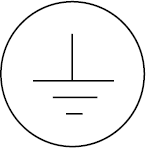
\includegraphics[width=1em]{fig/ground_symbol}
\end{itemize}

Before connecting the equipment to the mains of the building installation, the proper functioning of the protective earth lead of the building installation needs to be verified.

\begin{center}
\fbox{
\parbox{0.95\textwidth}{
\textbf{WARNING}: Any interruption of the protective conductor inside or outside the instrument, or
disconnection of the protective earth terminal, is likely to make the instrument dangerous.
Intentional interruption is prohibited.
}}
\end{center}

\subsubsection{Mains Voltage Cord and Fuses}
Different power cords are available for the various voltage outlets.

\textbf{Note:}
If the mains plug has to be adapted to the local situation it should only be done by a qualified
person.

This instrument is equipped with a tap-less switch mode power supply that covers most nominal
voltage ranges in use: 90-240V AC RMS. This obviates the need to adapt to the local mains voltage.

The mains frequency is 48-65 Hz.

\begin{center}
\fbox{
\parbox{0.95\textwidth}{
\textbf{WARNING}: This instrument shall be disconnected from all voltage sources when renewing a fuse.
}}
\end{center}

\textbf{Mains fuse rating:} 1.6 A delayed action, 250 V

The mains fuseholder is located on the rear panel of the instrument.

\textbf{If the mains fuse has to be replaced please proceed as follows:}
\begin{enumerate}
\item Remove the mains cable
\item Lift the plastic cover (fuseholder) by means of 2 small screwdrivers (simultaneously)
\item Insert the new fuse into the top of the fuseholder
\item Re-insert the cover (fuseholder)
\end{enumerate}

\begin{center}
\fbox{
\parbox{0.95\textwidth}{
\textbf{WARNING}: Make sure that only fuses of the required rating, voltage, and of the specified type are
used for replacement.

The use of repaired (jumped) fuses and/or the short-circuiting of the fuse holder is prohibited.

Fuses must only be replaced by a qualified person who is aware of the hazards involved.
}}
\end{center}

\subsection{Rack Mounting}
This PTV instrument is delivered in a 19'' cabinet. Four selfadhesive rubber feet are supplied together with this instrument

If several cabinets are mounted in a 19'' rack, special attention must be paid to the temperature inside the rack.

The PT 5300 is equipped with cooling fan and air inlet on the front. in bottom and at sides.
If the PT 5300 is mounted between other instruments with high surface temperature, this cooling may not be sufficient. Under these circumstances, it is recommended to make space between the instruments, and to establish forced circulation (cooling) in the rack.

\subsection{Installation of Rack Mounting Kit, PM 8552}
The rack slides mount in any rack with a front-to-rear spacing between 18 and 27 inches.
Reserve clearance between the rear panel of the instrument and the cabinet panel for
connectors and to provide necessary air circulation.

\textbf{Mounting of Slide Tracks}
\begin{enumerate}
\item Mount the chassis section of the rack slide kit to the instrument with the snap latch at the rear. Make sure that the screws are secured.
\item Mount the rails using the hardware shown in the figure. Align the stationary sections both horizontally and in level.
\end{enumerate}

\textbf{Installing of the Instrument}
\begin{enumerate}
\item Pull the slide-out section to the fully extended position.
\item Insert the instrument chassis section into the slide-out sections.
\item Press the snap latches and push the instrument towards the rack frame until the latches snap into their holes.
\item Press the stop latches again and push the instrument totally into the rack.
\item Fix the instrument by means of the front panel screws.
\end{enumerate}

After installation, the slide tracks might need to be slightly adjusted to ensure smooth operation.
To do so, pull the instrument halfway out, slightly loosen the screws holding the tracks to the front rail, and allow the tracks to settle to an unbound position. Tighten the screws and by pulling the instrument in and out several times ensure smooth operation.

\begin{figure}[hbt]
\centering
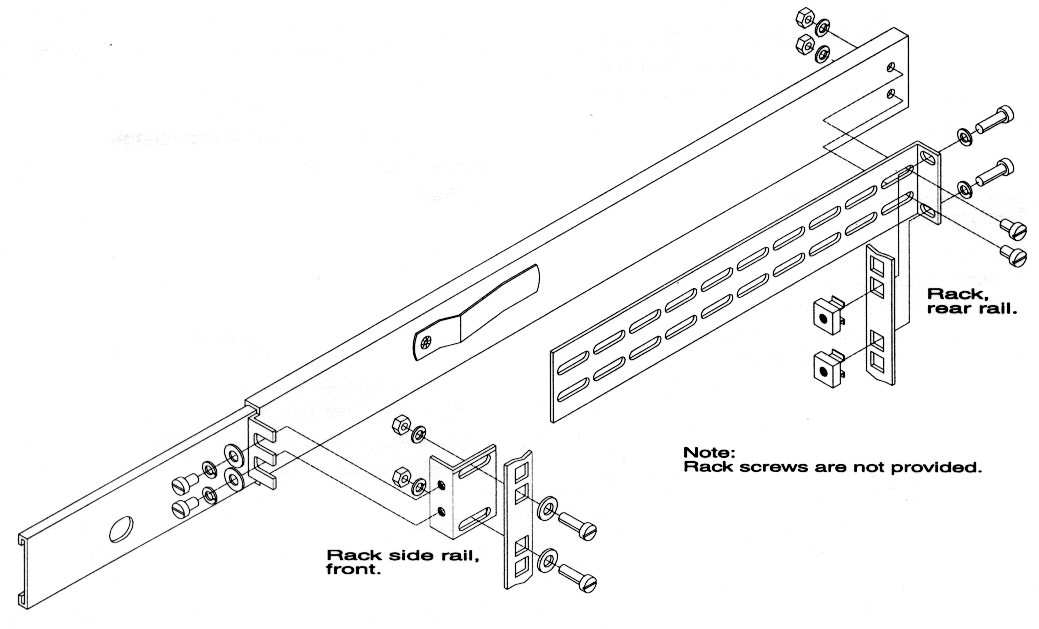
\includegraphics[width=\textwidth]{fig/rack}
\caption{Installation of PM 8552}
\end{figure}

\textbf{Removal of the Instrument}

Be sure that all cabling is disconnected before removing the instrument.
\begin{enumerate}
\item Loosen the screws in the rack frame and pull the instrument forward until the stop latches snap into their holes.
\item Press the stop latches and remove the instrument.
\end{enumerate}

\subsection{Cleaning}
\begin{itemize}
\item Disconnect the instrument from the mains voltage supply before cleaning
\item Use only a damp cloth
\item Make sure that no liquid is spilled inside the instrument
\end{itemize}

\subsection{Configuration}
\subsubsection{Remote Interface}
Move cable from connector SER (XR1) to PAR (XM1) on Main Board (Unit 1) to change from standard RS232 to simple ground-closure.

\begin{figure}[hbt]
\centering
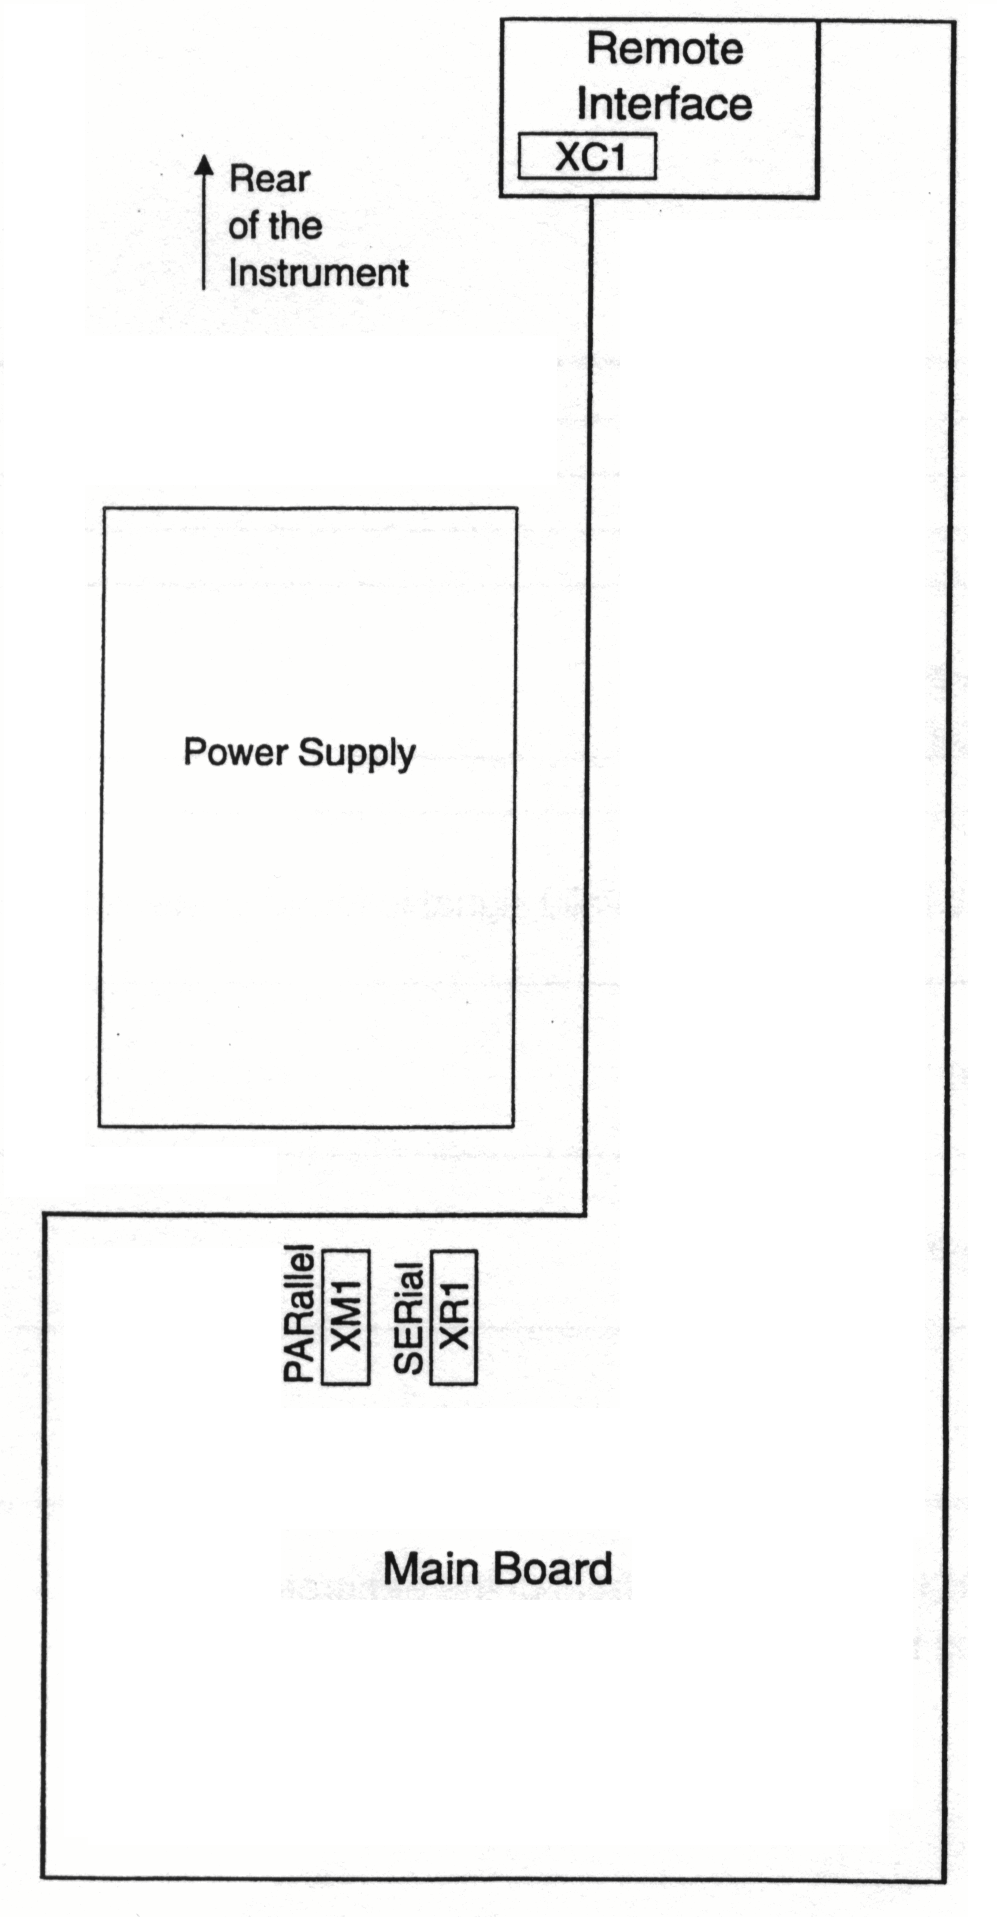
\includegraphics[width=0.5\textwidth]{fig/PT5300_overview}
\caption{Location of Connectors SER and PAR}
\label{serialconnector}
\end{figure}

\subsection{Access to and Replacement of Parts}
\subsubsection{Safety}
The opening of covers or removal of parts, expect those to which access can be gained by hand, is liable to expose live parts.

The instrument must be disconnected from all voltage sources before performing any adjustment, replacement, maintenance, or repair, which requires the instrument to be opened. If repair of the opened instrument is unavoidable, it must only be carried out by a skilled person who is aware of the hazards involved. To guarantee safety only original spare parts must be used.

\subsubsection{Access to the Units}
To gain access to the units, remove the screws that secure the top cover of the instrument and lift the cover up.

\subsubsection{Installation of Options}
The installation instruction is supplied with the option.
\clearpage
\subsection{GPS Antenna and cable connection}

The PT8616 option is delivered with an active antenna and 12 meters of cable selected for the unit. Some customers however may want to use their own antenna or run longer cables. This section explains what to look out for.

\textbf{Antenna requirements and specifications.}\\
The application always requires an active antenna, running 3.3 volts. There are two types of active antennas, which may be considered. Helix or Patch. The difference are the physical design and the area of the sky which is covered. A Helix antenna has a physical shape of a pole and covers the widest area of the sky. It also has to be physically bigger, to pick up RF signals, compared to the Patch antenna. The Patch antenna can be smaller but does not cover the sky just as well as the Helix antenna. The Helix antenna may be preferred on buildings, because of the slightly better performance, but the Patch antenna suits most needs and also fits well on OB vans, roofs etc.

Different antennas have different gains which will permit different cable lengths. The typical gain level is about +30 dB. An active antenna draws current in the region of 5 - 20 mA. It is important not to draw more current than 50 mA to avoid damaging the GPS circuit. In the case of short circuit the GPS receiver shuts down the supply voltage.

\textbf{Cable loss budget.}\\
It is very important the cable loss is considered carefully when using custom cables longer than the 12 meter RG58 cable supplied. The GPS RF frequency is 1575 MHz, so all further loss calculations will be at this specific frequency. 

The GPS receiver requires a minimum signal strength of -140 dBm to lock to a satellite. The GPS satellites are specified to deliver signals strengths between -123 dBm and -130 dBm at the earth surface. With a typical antenna  gain of 30 dB, the power level out of the antenna is in the range of -97 dBm. This allows a maximum loss of 43 dB in the cable, before the locking threshold of -140 dBm is reached. It is advisable to keep a margin of about 5 dB from the locking threshold. Clouds, snow and rain will degrade the performance.
Below are some examples of cable losses:

\begin{table}[hbt]
\centering
\begin{tabular}{|l|l|l|}
\hline
\textbf{Cable type} & \textbf{Loss/100 m @ 1.5 GHz} & \textbf{Max lenght, 35 dB loss} \\ \hline
\textbf{RG58}		& ~110 dB* & 31 m  \\ \hline
\textbf{RG213}	& ~44 dB*  & 75 m  \\ \hline
\textbf{CDF400}	& 17.8 dB  & 195 m \\ \hline
\end{tabular}\\
\textit{*) Note: The RG58 and RG213 are found in various low-loss versions.\\See datasheet for specific cable used.}
\caption{Cable types.}
\label{tab:cabletypes}
\end{table}

\textbf{Antenna and cable installation and usage.}\\
The placement of the antenna is important for the overall performance. The antenna must not be obstructed in any way. This obstruction could be caused by trees, roofs etc. What may seem less obvious is tall walls near the antenna which may decrease the performance. This is because the RF-signal may reflect of the wall and the antenna could receive both the direct and reflected signals which may confuse the receiver circuit. Always install the antenna where there is a clear sky-view.

Please note it is important the cable is connected to both the antenna and the PT5300 antenna input, before the unit is powered up. The GPS receiver calculates the noise floor on power-up and the connection with the antenna has to be established at this moment.

On power up, check that the text ``GPS: none'' on the front display changes to ``GPS: ok'' after a short time. This will confirm the connection works correctly. The final step is to seal the connection to prevent corrosion, when exposed to humidity.

\textbf{Electrical requirements.}\\
\textbf{Antenna.}\\
\spectabular
\textbf{Antenna voltage:}										& 3.3 Volts\\
\textbf{Antenna maximum power consumption:}	& 50 mA \\
\textbf{Antenna minimum gain:}							& 15 dB\\
\textbf{Antenna maximum gain:}							& 50 dB\\
\textbf{Antenna maximum noise figure:}			& 1.5 dB\\
\end{tabular*}

\textbf{Receiver.}\\
\spectabular
\textbf{Receiver input level:}				& -140 dBm < \textit{input} < -5 dBm \\
\textbf{Receiver input RF frequency:}	& 1575.42 MHz \\
\end{tabular*}

\clearpage
\clearpage
\section{Operating Instructions}

\subsection{General Information}
All operational controls and configurations are conveniently carried out from the front panel.

The two-line-by-40-characters LCD display, in conjunction with 4 cursor keys and an \EXECUTE button, allows easy and intuitive operation of the PT 5300 HD-SD Varitime\TM Sync Generator.

The cursor keys are used to call relevant menus on the display: the top line of the display shows the current status/selection or other current menu choices.

In the upper right corner of the display is an indication of cursor keys used in the active menu.
\begin{itemize}
\item a \rightbuttontext  indicate that the right arrow buttons can be used
\item a \upbuttontext  indicates that the up button can be used
\item a \downbuttontext  indicates that the down button can be used
\item a \leftbuttontext  indicate that the left arrow buttons can be used
\item and an \execute  indicates that the \EXECUTE button can be used
\end{itemize}

The bottom line of the display indicates new selections or enables changes to parameter setting.

\subsection{Front Panel Controls}
\subsubsection{Navigation Key}
The circular key in the middle of the front panel is the so-called Navigation key or Compass key is the tool for making the navigation through the menus light and easy.

\textbf{Note:} The function of some of the output/input connectors on the rear panel depends upon the functional modules/options included your generator and the functional configuration.

\begin{figure}[hbt]
\centering
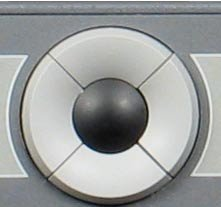
\includegraphics[width=0.2\textwidth]{fig/arrow_button}
\caption{PT5300 Navigation Keys}
\end{figure}

The black key in the middle is the \EXECUTE

The \upbuttontext (upper) button allows the user to exit the current menu and enter a higher-level menu, or to change parameter.

The \downbuttontext (lower) button allows the user to select new menus or sub-menus, or to change parameters.

The \leftbuttontext and \rightbuttontext (left and right) keys are used to scroll horizontally in the menus and to select the individual characters when naming presets an written text into the video full field test signals.

\paragraph{PRESET}
The \textbf{PRESET} button provides fast access to the instrument presets when switching between different standard applications.

\paragraph{OUTPUT}
The \textbf{OUTPUT} button provides a fast access to output signal selection on the generators.

\paragraph{GENLOCK}
The \textbf{GENLOCK} button provides a fast switching between locked and unlocked mode. The green LED next to the button indicates that \textbf{GENLOCK} has been selected. The type of genlock is selected via the menu.

\subsection{Indicators and Connections}
\subsubsection{Front Panel Indicators}
\paragraph{POWER ON}
A green LED that indicates when DC power is available from the internal DC supply.

\paragraph{WARNING}
A red LED indicates that the instrument has detected an irregularity. A more thorough description is given in the display. More errors if any can be found in the error log function.

\paragraph{UNLOCKED}
A red LED that indicates when genlock mode is enabled but no correct genlock signal is found on the active genlock input. In this case, the generator switches automatically to internal mode until a valid genlock signal becomes available.

\textbf{Note:} The function of some of the output/input connectors on the rear panel depends upon the functional modules/options included your generator and the functional configuration.

\begin{figure}[hbt]
\centering
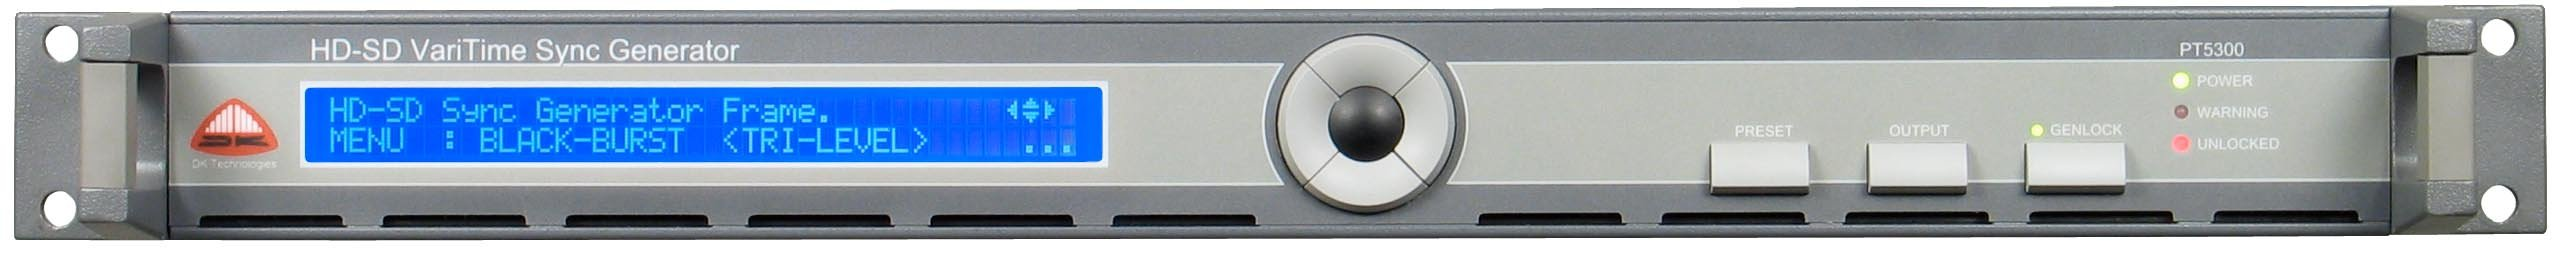
\includegraphics[width=0.8\textwidth]{fig/PT5300_front}
\caption{Front panel}
\end{figure}

\subsection{Display Information}
To guide the user through operations, symbols of the push buttons, which can be activated at a particular time will appear on the right side of the display.

\begin{tabular}{l p{24em}}
\upbuttontext \downbuttontext \leftbuttontext \rightbuttontext & Indicates which of the buttons in the Navigation are active \\
\execute &	Indicates that the \EXECUTE button (the black in the middle) must be pressed to activate the required selection \\
$< >$			& Indicates the position of the cursor on the menu line \\
$[$ $]$			& Indicates that changes to individual characters or digits are possible in timing and naming menus \\
\ldots		& Indicates that more items are available on the menu line \\
\locked		& Indicates that the panel is locked. Four different locked modes are available. The padlock will be only visible when the ``performed'' function is locked \\
\escape		& To abandon changes, place the cursor on \escape and press also \upbutton \\
\save			& To save a changed parameter, place the cursor on \save and press the \execute button \\
\end{tabular}

\subsection{Rear Panel Connections}

\textbf{Note:} The function of some of the output/input connectors on the rear panel depends upon the functional modules/options included your generator and the functional configuration.

\begin{figure}[hbt]
\centering
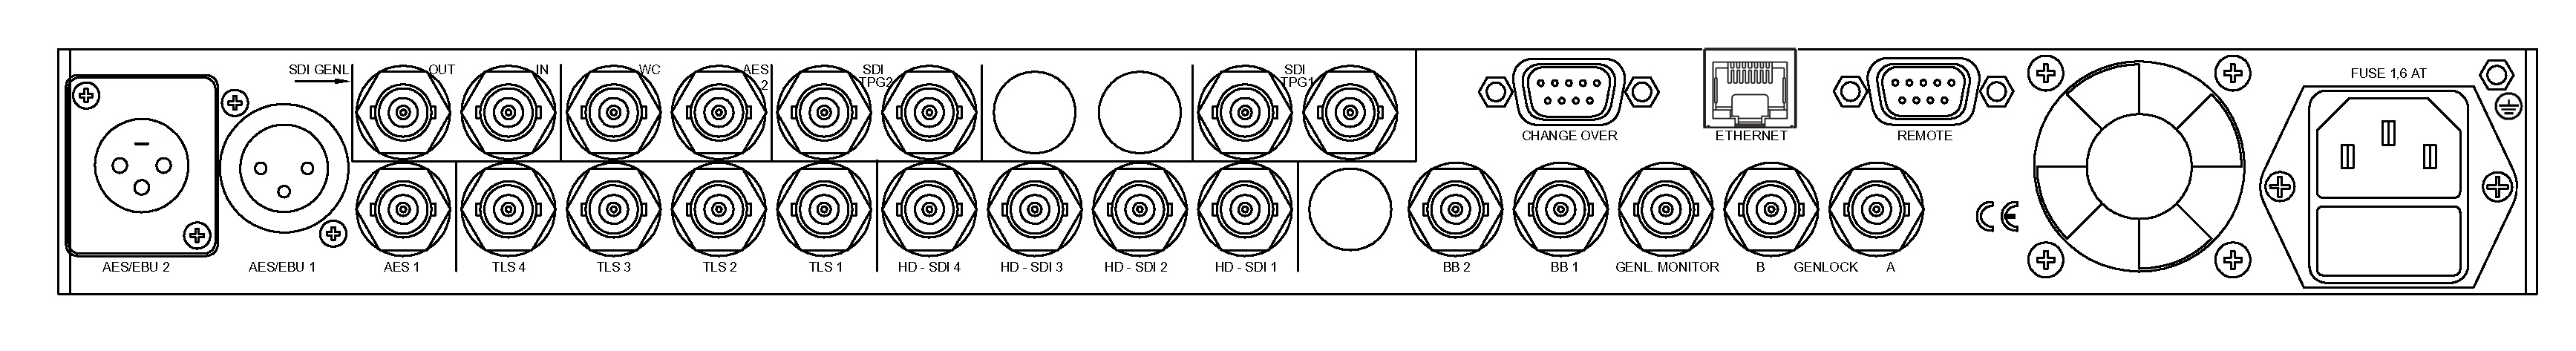
\includegraphics[width=\textwidth]{fig/PT5300_rear_view}
\caption{Rear panel}
\end{figure}

\textbf{Safety Ground (chassis)}

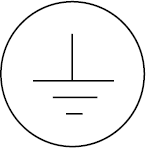
\includegraphics[width=2em]{fig/ground_symbol}

\textbf{On/Off button}

Mains switch

\begin{tabular}{l l}
ON:		& When ``I'' is pressed\\
OFF:	& When ``O'' is pressed\\
\end{tabular}

\textbf{Mains Connector}

Mains voltage receptacle.

\textbf{REMOTE}
Connector for remote control of the modulator. The remote connector can be configured either as standard RS 232 or as simple groundclosure. The configuration is done internally on the Main Board - Unit 1, please see page \pageref{serialconnector} for location. The instrument is set to RS 232 from factory.

\textbf{Ground-Closure Remote}

When the remote connector is configured for parallel ground-closure control a limited number of function can be controlled. Refer to chapter \ref{cha:Remote}.

\textbf{CHANGEOVER}

Remote connector to connect the PT 5300 HD-SD Varitime\TM  Sync Generator directly to a PT 5211 VariTime\TM  Sync Changeover Unit. This connector is used in set-up where a HD-SD Varitime\TM  Sync Generator is applied as back-up for a PT 5210 VariTime\TM  Digital Sync Generator and an automatic changeover unit.

\textbf{ANALOGUE GENLOCK A/B}

Two analogue genlock inputs included as standard. The inputs can be configured either as looped through or 75 \ohm  terminated.

\textbf{GENLOCK MONITOR}

Buffered 75 \ohm  output of the selected genlock signal. The signal is AC-coupled. 

\begin{multicols}{2}
{
\centering

\begin{tabular}{|p{0.42\textwidth}|}
\multicolumn{1}{p{0.42\textwidth}}{\textbf{BB1 and BB2}}\\
\hline
Two standard included outputs with Black Burst signals. \\
\hline
\end{tabular}

\begin{tabular}{|p{0.42\textwidth}|}
\multicolumn{1}{p{0.42\textwidth}}{\textbf{SDI-TPG1}}\\
\hline
\textbf{Output Options:} \\
Not included \\
One pair of SDI Test Pattern outputs\\
\hline
\end{tabular}

\begin{tabular}{|p{0.42\textwidth}|}
\multicolumn{1}{p{0.42\textwidth}}{\textbf{HD-SDI1 - HD-SDI2 - HD-SDI3 - HD-SDI4}}\\
\hline
\textbf{Output Options:}\\
Not included\\
Quad HD Tri-Level output\\
Quad HD-SD-SDI test signal out\\
Dual Link test output\\
One pair of SDI Basic Test Signals\\
One pair of SDI Test Pattern\\
One Pair of Analogue Test Patter\\
\hline
\end{tabular}

\begin{tabular}{|p{0.42\textwidth}|}
\multicolumn{1}{p{0.42\textwidth}}{\textbf{TLS1- TLS 2- TLS3- TLS4}}\\
\hline
\textbf{Output Options:}\\
Not included\\
Quad HD Tri-Level output\\
Quad HD-SD-SDI test signal out\\
Dual Link test output\\
One pair of SDI Basic Test Signals\\
One pair of SDI Test Pattern\\
One Pair of Analogue Test Pattern\\
\hline
\end{tabular}

\begin{tabular}{|p{0.42\textwidth}|}
\multicolumn{1}{p{0.42\textwidth}}{\textbf{AES/EBU2}}\\
\hline
\textbf{Output Options:}\\
Not included\\
AES/EBU digital audio test signal\\
Time code Input. (see (TIMECODE))\\
\hline
\end{tabular}

\begin{tabular}{|p{0.42\textwidth}|}
\multicolumn{1}{p{0.42\textwidth}}{\textbf{SDI GENLOCK IN/OUT}}\\
\hline
\textbf{Output Options:}\\
Not included\\
Active loop-through SDI genlock input\\
Special Configuration: AES/EBU and Wordclock\\
\hline
\end{tabular}

\begin{tabular}{|p{0.42\textwidth}|}
\multicolumn{1}{p{0.42\textwidth}}{\textbf{AES2}}\\
\hline
\textbf{Output Options:}\\
Not included\\
AES/EBU digital audio test signal output\\
\hline
\end{tabular}

\begin{tabular}{|p{0.42\textwidth}|}
\multicolumn{1}{p{0.42\textwidth}}{\textbf{WC}}\\
\hline
Not included\\
Wordclock, 48KHz, output\\
\hline
\end{tabular}

\begin{tabular}{|p{0.42\textwidth}|}
\multicolumn{1}{p{0.42\textwidth}}{\textbf{(TIME CODE)}}\\
\hline
\textbf{Input Options:}\\
Not included\\
\hline
Time Code\\
The time code signal is used as reference for the PT 8637 Time Clock Interface\\
\\
LTC\\
Pin 1: Ground\\
Pin2: Signal\\
Pin3: Signal\\
\\
1 Hz\\
Pin 1: Ground\\
Pin2: Connect externally to pin 1\\
Pin 3: Signal\\
\hline
\end{tabular}

\begin{tabular}{|p{0.42\textwidth}|}
\multicolumn{1}{p{0.42\textwidth}}{\textbf{GPS Genlock and LTC Generator}}\\
\hline
\textbf{Input / Output Options:}\\
Not included\\
GPS active amp input\\
LTC time code output\\
\hline
\end{tabular}
}
\end{multicols}

\textbf{Note:} The SPG's, the TSG's and TPG's can in principle be placed arbitrarily, but for correct correspondence between numbering in the display and on the rear plate, certain rules have to be followed.

\textit{The table \ref{table:pt5300_config} and figure \ref{figure:pt5300_config} show the possible combinations of Video Generators which can be installed}
	
\textbf{Note:} In most cases the output, HD-SDI 1, HD-SDI 2, HD-SDI 3, HD-SDI 4, have to be used before any of the outputs other outputs. In the TPG 1, out the PT8603 and PT8632 SDI Test Pattern Generators can be installed independently of the other generators, but not both at the same time.

% PT5300 config table
%\begin{table}
%{\tiny
%			
%\begin{tabular}{|p{0.5ex}|p{24.0ex}|p{0.5ex}|p{0.5ex}|p{0.5ex}|p{0.5ex}|p{0.5ex}|p{0.5ex}|p{0.5ex}|p{0.5ex}|p{0.5ex}|p{0.5ex}|p{0.5ex}|p{0.5ex}|p{0.5ex}|p{0.5ex}|p{0.5ex}|p{0.5ex}|p{0.5ex}|p{0.5ex}|p{0.5ex}|p{0.5ex}|p{0.5ex}|p{0.5ex}|p{0.5ex}|p{0.5ex}|p{0.5ex}|p{0.5ex}|p{0.5ex}|}
%\hline
%\multicolumn{2}{|c|}{\multirow{3}{*}{ }} & \multicolumn{27}{|c|}{Inputs / Outputs} \\ \cline{3-29}
%\multicolumn{2}{|c|}{PT5300 Configuration Matrix} & \begin{sideways}{OUT}\end{sideways} &
%		\begin{sideways}{IN}\end{sideways} &
%		\begin{sideways}{WC}\end{sideways} &
%		\begin{sideways}{AES2}\end{sideways} &
%		\begin{sideways}{TPG2}\end{sideways} &
%		\begin{sideways}{TPG2}\end{sideways} &
%		\begin{sideways}{ }\end{sideways} &
%		\begin{sideways}{ }\end{sideways} &
%		\begin{sideways}{TPG1}\end{sideways} &
%		\begin{sideways}{TPG1}\end{sideways} &
%		\begin{sideways}{A}\end{sideways} &
%		\begin{sideways}{B}\end{sideways} &
%		\begin{sideways}{Mon.}\end{sideways} &
%		\begin{sideways}{BB1}\end{sideways} &
%		\begin{sideways}{BB2}\end{sideways} &
%		\begin{sideways}{ }\end{sideways} &
%		\begin{sideways}{HD-SDI1}\end{sideways} &
%		\begin{sideways}{HD-SDI2}\end{sideways} &
%		\begin{sideways}{HD-SDI3}\end{sideways} &
%		\begin{sideways}{HD-SDI4}\end{sideways} &
%		\begin{sideways}{TLS1}\end{sideways} &
%		\begin{sideways}{TLS2}\end{sideways} &
%		\begin{sideways}{TLS3}\end{sideways} &
%		\begin{sideways}{TLS4}\end{sideways} &
%		\begin{sideways}{AES1}\end{sideways} &
%		\begin{sideways}{AES1}\end{sideways} &
%		\begin{sideways}{AES2/LTC}\end{sideways}\\
%\multicolumn{2}{|l|}{ } &1&2&3&4&5&6&7&8&9&10&11&12&13&14&15&16&17&18&19&20&21&22&23&24&25&26&27\\ \hline
% 
%	\hline
%	\multirow{4}{*}{\begin{sideways}Base units\end{sideways}} 
%	& PT5300HD-SD Base Genlock A/B In/Out & & & & & & & & & & &X&X& & & & & & & & & & & & & & & \\ \cline{2-29}
%	& PT5300HD-SD Base Genlock A/B In/Out & & & & & & & & & & & & &X& & & & & & & & & & & & & & \\ \cline{2-29}
%	& PT5300HD-SD Base Genlock A/B In/Out & & & & & & & & & & & & & &X&X& & & & & & & & & & & & \\ \cline{2-29}
%	& PT5300HD Base Quad Tri-Level Sync out & & & & & & & & & & & & & & & & & & & & &X&X&X&X& & & \\ \cline{2-29}
%	\hline
%	\multirow{15}{*}{\begin{sideways}Optional Modules\end{sideways}} 
%	& PT8603 SD-SDI Test Signal Gen 			& & & & & & & & &X&X& & & & & & & & & & & & & & & & & \\ \cline{2-29}
%	& PT86046 parallel BB outputs 				& & & & & & & & & & & & & & & & & &X&X&X&X&X&X& & & & \\ \cline{2-29}
%	& PT8606 SDI genlock In / Out 				&X&X& & & & & & & & & & & & & & & & & & & & & & & & & \\ \cline{2-29}
%	& PT8608 Dual BB outputs 							& & & & &X&X& & & & & & & & & & & &O&O& & &O&O& & & & \\ \cline{2-29}
%	& PT8609 SDI Black \& C. Bar out 			& & & & &X&X& & & & & & & & & & & &O&O& & &O&O& & & & \\ \cline{2-29}
%	& PT8611 Quad Tri-Level Sync out 			& & & &O&O&O&O& & & & & & & & & &O&O&O&O&X&X&X&X& & & \\ \cline{2-29}
%	& PT8612 Quad HD-SD SDI out 					& & & & & & & & & & & & & & & & &X&X&X&X&O&O&O&O& & & \\ \cline{2-29}
%	& PT8613 Dual Link HD-SDI test out 		& & & & & & & & & & & & & & & & &X&X&X&X&O&O&O&O& & & \\ \cline{2-29}
%	& PT8616 GPS In , LTC Out 						& &X& & &O&O& & &O&O& & & & & & & & & & & & & & & & &X\\ \cline{2-29}
%	& PT8631 PAL/NTSC Test signal gen.		& & & & &X&X& & & & & & & & & & & & & & & & & & & & & \\ \cline{2-29}
%	& PT8632 SD-SDI Test Signal Gen. 			& & & & & & & & &X&X& & & & & & & & & & & & & & & & & \\ \cline{2-29}
%	& PT8633 SD-SDI Test Signal Gen. 			& & & & &X&X& & & & & & & & & & & & & &O&O& & & & & & \\ \cline{2-29}
%	& PT8635 Dual AES3 Audio Gen. 				& & &X&X& & & & & & & & & & & & & & & & & & & & &X& &X\\ \cline{2-29}
%	& PT8637 Time \& Clock interface 			& & & & & & & & & & & & & & & & & & & & & & & & & & &X\\ \cline{2-29}
%	& PT8639 SD-SDI Test Signal Gen. 			& & & & &X&X& & & & & & & & & & & & & &O&O& &O&O& & & \\ \cline{2-29}
%	\hline
%
%\end{tabular}
%
%}
%\caption{PT 5300 Configurations (X=Primary position, O=Additional/alternate position }
%\label{table:pt5300_config}
%\end{table}

\begin{figure}[hbt]

\centering

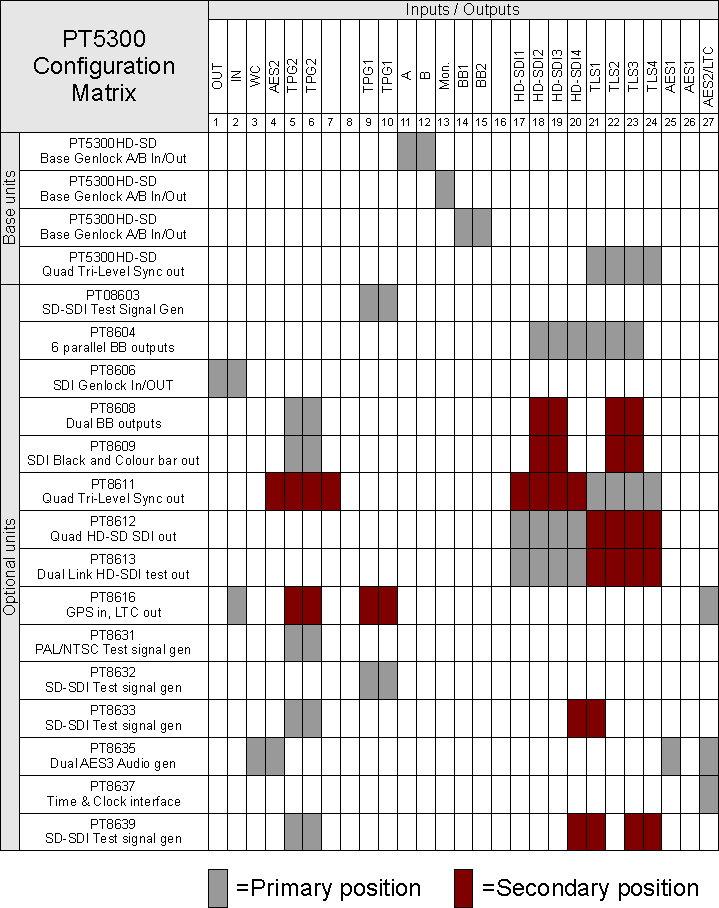
\includegraphics[width=0.8\textwidth]{fig/Config_matrix}

\caption{PT 5300 Configurations }
\label{table:pt5300_config}

\end{figure}

\textbf{Note:} The function of some of the output/input connectors on the rear panel depends upon the functional modules/options included your generator and the functional configuration.

\begin{figure}[hbt]
\centering
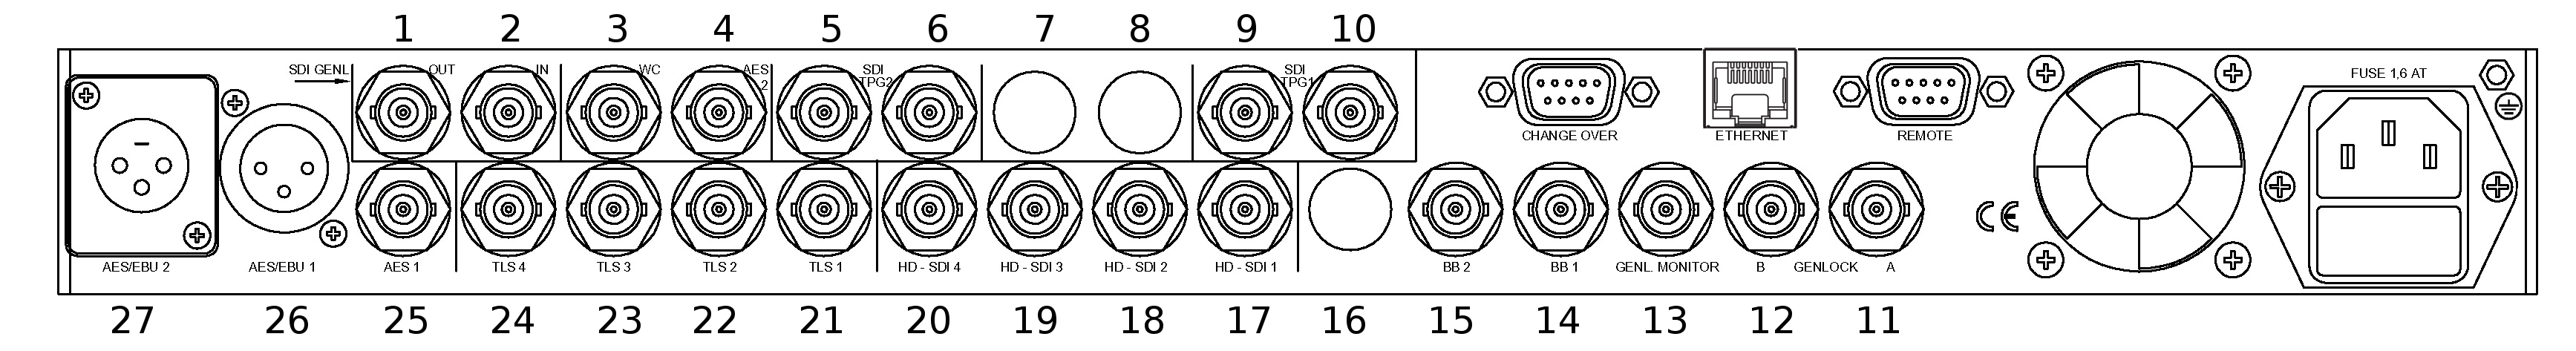
\includegraphics[width=\textwidth]{fig/PT5300_rear_config}
\caption{Rear Panel, Configuration}
\label{figure:pt5300_config}
\end{figure}

\subsection{Panel Operation}
The PT 5300 HD-SD Varitime\TM Sync Generator may be equipped with several different optional modules. The menu system always reflects the modules installed. The operation of each of the modules is described below, although it is impossible for all the modules to be installed in one instrument at one time.

\subsubsection{Power Up}
A diagnostic routine is performed at power-on. After a normal start-up, the HD-SD Varitime\TM Sync Generator continues to the status display. If a failure is detected an error message is displayed.

\paragraph{Normal Start-up}
\display{HD-SD Sync. Gen.Power-up diagnose}{Selftest in progress \ldots}

This message is shown while the test is performed.

\textbf{After a successful test the following message is shown:}

\display{HD-SD Sync. Gen. Frame}{Version: 07.-03.0}

The instrument stops if errors are detected.
The diagnose may be continued if you press the \upbuttontext, \downbuttontext, \leftbuttontext, \rightbuttontext or \execute .
When the power-up diagnose program is finished, the instrument may be used, but excluding the erroneous function(s).

%\textit{Please see Appendix xxx for the list of errors detectable during power-up.}

\subsubsection{Status Displays}
If a preset was active at the previous power-down, this preset is automatically recalled and the preset status display is shown. The preset status display shows the number and name of the active preset.

\display{HD-SD Preset Status \leftbutton \downbutton \rightbutton}{PRESET (6):name of preset}
If genlock is activated in the preset and no genlock signal is identified, the status display will change to the genlock status display indicating UNLOCKED.

If no preset is active then genlock status display will be displayed.

Use the \leftbuttontext and \rightbuttontext buttons to select the status displays you want.

\textbf{Note:} The status displays for the various options are only available when the options are
installed.









\paragraph{Status:Preset}
\display{HD-SD Preset Status \leftbutton \downbutton \rightbutton}{NO PRESET ACTIVE}
\display{HD-SD Preset Status \leftbutton \downbutton \rightbutton}{PRESET (1):name of preset}

\paragraph{Status: Genlock}
\display{Genlock:A \leftbutton \downbutton \rightbutton}{Signal:PAL Burst Status: GENLOCKED}
\display{Genlock:Internal \leftbutton \downbutton \rightbutton}{Signal:-------Status:-------}

The genlock status display shows the input selected for genlock and the format of genlock selected. If the signal is NTSC or PAL the display will also indicate whether sync lock or burst lock is being used.

\textbf{Status: Analogue test pattern generator}

\display{Analog TPG1:PLUGE \leftbutton \downbutton \rightbutton}{System:PAL w/PAL ID +TEXT}

The status display for the analogue test pattern generator shows the signal output from each the generator and the system selected. If the text or time clock is inserted into the test pattern, then the presence is shown.

\textbf{Status: SDI test pattern generator}

\display{SDI-TPG1:PLUGE \leftbutton \downbutton \rightbutton}{System:525/59.94.+TEXT +AUDIO +EDH}

The status display for serial digital test pattern generator shows the signal output from each generator and the system selected. Also the status for text (and clock), embedded audio, and EDH inserted into test signals/pattern is shown.

\textbf{Status: SDI Basic generator}

\display{SDI-TSG3:WINDOW 15\% \leftbutton \downbutton \rightbutton}{System:525/59.94. +AUDIO +EDH}

The serial digital test signal generator status display shows the signal output from each of the Basic SDI generators and the system selected. Also the status for embedded audio and EDH is shown. No text or clock can be inserted.

\textbf{Status: AES/EBU Audio Generator}

\display{AES/EBU1:Stereo EBU 1kHz \leftbutton \downbutton \rightbutton}{Level:-9dBFS Timing:PAL}

The status display for the AES/EBU digital audio generator shows the output signal and level of the audio. The five NTSC phases or the PAL timing phase is also displayed.

\textbf{Status: DATE-TIME}

\display{DATE:05-02-02 TIME:14:05:05 ?? \leftbutton \downbutton \rightbutton}{REF: VITC Code STATUS: LOCKED}
This display shows the current status of date and time i.e. the information inserted into the video signal.

\textbf{Status: WARNING}

\display{HD-SD Error/Warning Status:?? \leftbutton \downbutton \rightbutton}{No error detected}
\display{HD-SD Error/Warning Status:?? \leftbutton \downbutton \rightbutton}{No active warning}
\display{HD-SD Error/Warning Status:?? \leftbutton \downbutton \rightbutton}{E(00n):mmmmmmmmmm}

The display shows the error/warnings status. The ``No error detector'' shows that no errors has been detected. The ``No active warning'' shows that no errors are present, but previously detected errors are stored in the ``Errorqueue''. In case of an error condition, the error number is shown in the display.
%\textit{Please refer to Appendix xxx for explanation of error messages}










\subsubsection{Menu Operation}
Pressing the \downbuttontext button in the status menu will cause the main menu to appear. This is the main route of access to all functions. If the control panel is locked, the padlock symbol will be flashing. Depending on which type of lock is used, it may have to be removed before some operations are allowed.

\textbf{To exit the STATUS menu, press the \downbuttontext button and move to the main menu:}

\display{HD-SD Sync Generator \leftbutton \updownbutton \rightbutton}{<BLACK-BURST> TRI-LEVEL HD-SDI \ldots}
\display{HD-SD Sync Generator \leftbutton \updownbutton \rightbutton}{<DL-SDI> ANALOG SDI-TSG4 \ldots}
\display{HD-SD Sync Generator \leftbutton \updownbutton \rightbutton}{<SDI-TPG1> SDI-TPG2 SDI-TPG5 \ldots}
\display{HD-SD Sync Generator \leftbutton \updownbutton \rightbutton}{<SDI-TPG2> AES-EBU <GENLOCK> \ldots}
\display{HD-SD Sync Generator \leftbutton \updownbutton \rightbutton}{LTC PRESET <CONFIG> \ldots}

\textbf{Note:} Not all of the above options can be installed at a time; maximum 2 HD-SD SDI boards and/or up to
3 TRI-LEVEL-SYNC and/or up 4 TSG's and/or up to 3 TPG's can be mounted at a time. For the
possible combinations, refer to figure \ref{figure:pt5300_config}. If one or more of the options is not installed, the keyword will be missing in the menu.

\textbf{Select one of the menus and go on to the next menu, e.g.:}

\display{MENU:BLACK-BURST, configure \leftbutton \updownbutton \rightbutton}{SUBMNU:<BB1> BB2}

The menus have basically the same structure and the same procedure is used with all the menus.
Select one of the items in the menu displayed
\begin{itemize}
\item Make a selection in the next menu below
\item Use the arrow buttons as indicated in the icon field
\item Select \save and press \execute to store the setting Select ESC and press \upbuttontext button to escape the menu or
\item Select the next menu level, i.e. 2NDMNU or
\item Confirm the selection by pressing \EXECUTE %(E is shown in the icon area)
\end{itemize}

\textbf{Note:} \save does not appear until a parameter is changed. Unintended changes are cancelled by selecting ESC and returning to the level above.

\subsection{Detailed Description of Menus}






\subsubsection{Menu: BLACK-BURST generator}
This is the menu for setting the parameters for the analogue Black Burst outputs. The analogue Black Burst outputs are named BB1 and BB2 connector on the back of the instrument.

\textbf{Setting of the BLACK-BURST generator:}

\display{MENU:BLACK-BURST, configure \leftbutton \updownbutton \rightbutton}{SUBMNU:<BB1>BB2}

\begin{itemize}
\item Use the \leftbuttontext and \rightbuttontext buttons to select BB1
\item Then press \downbuttontext to enter the submenu for BB1
\end{itemize}

\display{SUBMNU:BLACK-BURST/BB1,select \leftbutton \updownbutton \rightbutton}{2NDMNU:<SYSTEM> TIMING ScH-PHASE}
The 2NDMNU allows changes to be made in the parameters for the BB1 output.

\textbf{To change form NTSC to PAL, select SYSTEM}

\display{2NDMNU:../BB1/SYSTEM, select \leftbutton \updownbutton \rightbutton}{SYSTEM:<PAL w/PAL ID> SAVE ESC}

\textbf{Operation:}

\begin{itemize}
\item Use the \upbuttontext and \downbuttontext buttons to find the system setting you want.
\item When the desired system appears in the display, move the cursor to \save and press \EXECUTE to change the system setting
\item If no change is desired, move the cursor to ESC and press \upbuttontext
\end{itemize}

\textit{Leaving the function takes you back to the BLACK-BURST/BB1 submenu.}

\textbf{Analogue Black Burst generator system options:}

\begin{itemize}
\item NTSC
\item PAL
\item PAL w/PAL ID
\end{itemize}

\textbf{Note:} If the PAL Field 1 pulse in Line 7 is inserted, it is independent of the Sc-H phase setting. If the Sc-H phase has been adjusted, the Line 7 pulse will identify the field as if the phase had not been changed from the nominal setting.
When the system ``PAL w/PAL ID'' is selected, a pulse indicating PAL Field 1 is included Line 7.

\textbf{Note:} When changing the system from PAL to NTSC you must check the timing adjustment: a valid PAL timing may NOT be valid in NTSC. If the timing is not valid in NTSC then it will be reset to +0,+0,+0.

\textbf{To change the delay/advance timing for the BB1 output, select TIME.}

\display{2NDMNU:../BB1/TIMING, edit delay \leftbutton \updownbutton \rightbutton}{V:<+1> H:+008 T: +00124.3 SAVE ESC}

\textbf{Operation:}

\begin{itemize}
\item Use the \leftbuttontext or \rightbuttontext buttons to select V, H, or T
\item Then use the \upbuttontext and \downbuttontext buttons to change the setting changes to the timing are instantaneous, i.e. any changes are reflected immediately in the output signal
\item When the desired setting appears in the display, move the cursor to \save and press \EXECUTE to change the setting
\end{itemize}

The timing can be adjusted by coarse or fine adjustment parameters. The coarsest adjustment is field (V) the finest is time (T), and line (H) is in between. The T value is in nanoseconds.
\begin{itemize}
\item The T value can be changed by using the \upbuttontext and \downbuttontext buttons to adjust the smallest step for the adjustment, but a faster method is to press \EXECUTE when the cursor is on the T value. This opens an editor in which each of the time digits can be changed using the \upbuttontext and \downbuttontext buttons
\item Positions are Selected by using the \leftbuttontext and \rightbuttontext buttons
\item To exit the editor press \EXECUTE
\item When the desired delay setting appears in the display, move the cursor to \save and press \EXECUTE
\item If no changes are desired, move the cursor to ESC and press \upbuttontext
\end{itemize}

\textit{Leaving the function takes you back to the BLACK-BURST/BB1 submenu.}

\textbf{To change the Sc-H phase of the BB1 output, select ScH-PHASE}

\display{2NDMNU:../BB1/SCH-PHASE, EDIT \leftbutton \updownbutton \rightbutton}{ScH-PHASE:<+5deg> SAVE ESC}
The default Sc-H phase for the BB outputs is 0 degrees. The value can be changed in steps of 1 degree.

\textbf{Operation:}

\begin{enumerate}
\item Use the \upbuttontext and \downbuttontext buttons to change the Sc-H phase. Change to the Sc-H phase is instant, i.e. any change made in the display is reflected immediately in the output signal
\item When the desired setting appears in the display, move the cursor to \save and press
\item EXECUTE
\item If no change is desired, move the cursor to ESC and press \upbuttontext
\end{enumerate}
\textit{Leaving the function takes you back to the BLACK-BURST/BB1 submenu.}








\subsubsection{Menu: TRI-LEVEL sync generator}
This is the menu for setting the parameters for the analogue TRI-LEVEL SYNC outputs.

The analogue TRI-LEVEL outputs are named TLS1, TLS2, TLS3, TLS4 when the units is
mounted in the primary position and TLS5, TLS6, TLS7, TLS8 when the units is mounted in the
additional / alternate position as mentioned in the table 6-1 on page 6-30

\textbf{Setting of the TRI-LEVEL SYNC generator:}

\display{MENU:TRI-LEVEL, configure \leftbutton \updownbutton \rightbutton}{SUBMNU:<TLS1> TLS2 TLS3 TLS4}

\begin{itemize}
\item Use the \leftbuttontext and \rightbuttontext buttons to select TLS1
\item Then press \downbuttontext to enter the submenu for TLS1
\end{itemize}

\display{SUBMNU:TRI-LEVEL/TLS1,select \leftbutton \updownbutton \rightbutton}{2NDMNU:<SYSTEM> TIMING}
The 2NDMNU allows changes to be made in the parameters for the TLS1 output.

\textbf{To change from one HD TRI-LEVEL format to another, select FORMAT}

\display{2NDMNU:../TLS1/SYSTEM, select \leftbutton \updownbutton \rightbutton}{SYSTEM:<HD 1080I/25> SAVE ESC}

\textbf{Operation:}

\begin{itemize}
\item Use the \upbuttontext and \downbuttontext buttons to find the format setting you want.
\item When the desired system appears in the display, move the cursor to \save and press \EXECUTE to change the format setting
\end{itemize}

\display{2NDMNU:../TLS1/SYTEM, select \leftbutton \rightbutton \execute}{SYSTEM:HD 1080I/25 <SAVE> ESC}

\begin{itemize}
\item If no change is desired, move the cursor to ESC and press \upbuttontext
\end{itemize}

\textit{Leaving the function takes you back to the TRI-LEVEL/TLS1 submenu.}

\textbf{Analogue TRI-LEVEL SYNC generator system options:}

\begin{itemize}
\setlength{\itemsep}{1pt}
\setlength{\parskip}{0pt}
\item 1080p/60
\item 1080p/59.94
\item 1080p/50
\item 1080p/30
\item 1080p/29.97
\item 1080p/25
\item 1080p/24
\item 1080p/23.96
\item 1080i/30
\item 1080i/29.97
\item 1080i/25
\item 720p/60
\item 720p/59.94
\item 720p/50
\item 720p/30
\item 720p/29.97
\item 720p/25
\item 720p/24
\item 720p/23.9
\end{itemize}

\textbf{Note:} When changing from one format to the other you must check the timing adjustment, as the timing in one format may NOT be valid in a different format. If the timing is not valid then it will be reset to +0,+0,+0.

\textbf{To change the delay/advance timing for the TLS1 output, select TIMING.}

\display{2NDMNU:../TLS1/TIMING, edit delay \leftbutton \updownbutton \rightbutton \execute}{F:<+1> H:+008 T: +00006.7 SAVE ESC}

\textbf{Operation:}

\begin{itemize}
\item Use the \leftbuttontext or \rightbuttontext buttons to select F, H, or T
\item Then use the \upbuttontext and \downbuttontext buttons to change the setting. Changes to the timing are instantaneous, i.e. any changes are reflected immediately in the output signal.
\item When the desired setting appears in the display, move the cursor to \save and press \EXECUTE to change the setting.
\end{itemize}

The timing can be adjusted by coarse or fine adjustment parameters. The coarsest adjustment is field (F) the finest is time (T), and line (H) is lines. The T value is in nanoseconds.

\begin{itemize}
\item The T value can be changed by using the \upbuttontext and \downbuttontext buttons to adjust the smallest step for the adjustment, but a faster method is to press \EXECUTE when the cursor is on the T value. This opens an editor in which each of the time digits can be changed using the \upbuttontext and \downbuttontext buttons.
\item Positions are Selected by using the \leftbuttontext and \rightbuttontext buttons.
\item To exit the editor press \EXECUTE
\item When the desired delay setting appears in the display, move the cursor to \save and press \EXECUTE
\item If no changes are desired, move the cursor to ESC and press \upbuttontext
\end{itemize}

\textit{Leaving the function takes you back to the TRI-LEVEL/TLS1 submenu.}








\subsubsection{Menu: GENLOCK}
This is the menu for setting the genlock parameters, which are the common reference for theindividual timing of each generator.

It is always possible to genlock to analogue signals, while the PT 8606 SDI Digital Genlock option is necessary in order to genlock to digital video. The standard genlock inputs are designated A and B, and they can be either configured to signals terminated with 75 \ohm or configured as a high impedance loop-through.

The genlock function can be configured to different inputs and signals. Which signals are valid for each of the inputs depends on the setting in the Genlock menu.

\textbf{Select: GENLOCK}

\display{MENU : GENLOCK, select input \leftbutton \updownbutton \rightbutton}{<INTERNAL> SYS TIMING ESC}
\display{MENU : GENLOCK, select input \leftbutton \updownbutton \rightbutton}{<A PAL Burst> SYS TIMING OK ESC}

\textbf{Operation:}

\begin{itemize}
\item When an input has been configured to a specific type of genlock, this will be shown in the genlock select input menu
\item Use the \upbuttontext and \downbuttontext buttons to scroll through the different input options (with attached genlocked
types)
\item Then move the cursor to OK and press \EXECUTE button to change the selection (OK is only visible for other selections than the active)
\item If no change is desired, move the cursor to ESC and press \upbuttontext
\end{itemize}

\textit{Leaving the function takes you back to the GENLOCK menu.}

\textbf{The types of inputs available are:}

\begin{itemize}
\item A xxxxxx: Input A terminated 75 \ohm
\item B xxxxxx: Input B terminated 75 \ohm
\item A-B xxxxxx: Input A and B looped through, high impedance
\item Internal: The internal OCXO used as reference
\item SDI xxxxx: The optional PT 8606 SDI Digital Genlock module used for genlock input
\end{itemize}

Included with the selection is a description of the signal type used for the genlock. The xxxxxx reflects the genlock system selected in the SYStem submenu. For instance ``A-B PAL Burst'' indicates that loop-through A-B is configured for PAL burst lock.

\textbf{Note:} The ``UNLOCKED'' LED is ON when no correct genlock signal is found on the active genlock input.

\textbf{To change the genlock system for the input selected, select SYS in the GENLOCK menu.}

\display{SUBMNU:GENLOCK/SYSTEM, select \leftbutton \updownbutton \rightbutton}{SYSTEM:<PAL Burst> SAVE ESC}

\textbf{Operation:}

\begin{itemize}
\item Use the \upbuttontext and \downbuttontext buttons to select the system format of genlock for the input
\item  When the new format appears on the display, then move the cursor to \save and press \EXECUTE to change the signal format
\item  If no change is desired, move the cursor to ESC and press \upbuttontext 
\end{itemize}

\textit{Leaving the function takes you back to the GENLOCK menu.}

\textbf{Note:} Now the selected genlock system (A, B, Loop-through, Internal, or SDI) is configured. If the input for this system has not been activated, select OK in the GENLOCK menu and press \EXECUTE

Which signals are available to the different genlock inputs depends upon the type of genlock
edited.

\textbf{Genlock signals available for A, B, and A-B:}

\begin{itemize}
\setlength{\itemsep}{1pt}
\setlength{\parskip}{0pt}
\item PAL Burst
\item NTSC Burst
\item 625 Sync
\item 525 Sync
\item 4.43 MHz
\item 3.58 MHz
\item 5 MHz
\item 10 MHz
\end{itemize}

\textbf{Genlock signals available for SDI/GPS:}

\begin{itemize}
\item 525/59.94
\item 626/50
\end{itemize}

\textbf{Note:} No Genlock system nor Timing can be selected when Genlock Input is set to Internal or one of the continuous wave signals.

\textbf{To change the genlock timing for the input selected, select TIMING in the GENLOCK menu.}

\display{SUBMNU:GENLOCK/TIMING, edit delay \leftbutton \updownbutton \rightbutton}{V:<+0>H:+123 T:+00123.4 SAVE ESC}

\textbf{Operation:}

\begin{itemize}
\item Use the \leftbuttontext and \rightbuttontext buttons to select V, H, or T
\item Then use \upbuttontext or \downbuttontext buttons to select the value desired. Changes to the timing are instantaneous, i.e. any changes are reflected immediately in the output signal.
\end{itemize}

The timing can be adjusted by coarse or fine adjustment parameters. The coarsest adjustment is the Field (V), the finest is Time (T), and Line (H) is between. The T value is in nanoseconds. The timing resolution depends upon the type of signal used for genlock. 

\begin{itemize}
\item When the desired delay setting appears in the display, move the cursor to \save and press \EXECUTE
\item If no change is desired, move the cursor to ESC and press \upbuttontext 
\end{itemize}

\textit{Leaving the function takes you back to the GENLOCK menu}

\textbf{Note:} The genlock timing can only be changed when the genlock type is a signal containing line and field information. It is not possible to change timing when the reference is 5/10 MHz, Subcarrier frequency or internal.

\textbf{Note:} When changing genlock signal format, for instance, from PAL to NTSC, the timing parameters may become invalid: The timing parameter will then be reset to 0 for the input in question.









\subsubsection{Menu: GPS Genlock and LTC output}
This is the menu for setting the parameters for the GPS Genlock input and the LTC outputs.

\textbf{Select: GENLOCK}

\display{MENU : GENLOCK, select input \leftbutton \updownbutton \rightbutton}{<INTERNAL> SYS TIMING ESC}
\display{MENU : GENLOCK, select input \leftbutton \updownbutton \rightbutton}{<GPS 625/50> SYS TIMING OK ESC}

\textbf{Operation:}

\begin{itemize}
\item When an input has been configured to a specific type of genlock, this will be shown in the genlock select input menu
\item Use the \upbuttontext and \downbuttontext buttons to scroll through the different input options (with attached genlocked types)
\item Then move the cursor to OK and press \EXECUTE button to change the selection (OK is only visible for other selections than the active)
\item If no change is desired, move the cursor to ESC and press \upbuttontext Leaving the function takes you back to the GENLOCK menu.
\end{itemize}

\textit{Leaving the function takes you back to the GENLOCK menu.}

The LTC outputs are named LTC A and LTC B. LTC A and LTC B are output to both BNC connectors at the same time where on the XLR connector it is one at the time.

\textbf{Settings of the LTC generator:}

\display{SUBMNU: LTC, select 13:55:09 \leftbutton \updownbutton \rightbutton}{LTC A <OFFSET> FORMAT TIME SYNC ESC}

\begin{itemize}
\item Use the \upbuttontext and \downbuttontext buttons to switch between LTC A or B set-up, when marked as shown above. Notice, that switching between LTC A and B, only determines which generator to be setup, and does not yet alter the outputs.
\item Select the parameter, you wish to change, then press \downbuttontext to enter the parameter submenu for the selected LTC generator.
\end{itemize}

\textbf{To set offset, select OFFSET:}

\display{2NDMNU: ../LTC A/OFFSET, edit delay \leftbutton \updownbutton \rightbutton}{OFFSET: <+0000100000.0>ns OK ESC}

Each LTC generator can be individually timed, relative to absolute (GPS) time. The offset can be in the range of $\pm$500 ms, in steps of 6.7 ns.

\textbf{Operation:}

\begin{itemize}
\item Use the \upbuttontext and \downbuttontext buttons to increase/decrease delay. Pressing OK will apply the delay.
\item For faster adjustment, you can go into coarse mode. By pressing the \execute button, you can edit the individual digits. Select a digit by pressing 3 and 4, and edit the offset, by pressing \updownbuttontext. Notice, that the lowest digit cannot be selected. This is because the step-size is greater than what this digit represents.
\item When done, move the cursor to OK and \EXECUTE or move to ESC and press \upbuttontext to cancel. 
\end{itemize}
\textit{Leaving the function takes you back to the LTC submenu.}

\textbf{To change between formats, select FORMAT}

\display{2NDMNU: ../LTC A/FORMAT, select \leftbutton \updownbutton \rightbutton}{FORMAT: <25.00 FPS> SYNCMODE OK ESC}

\textbf{Operation:}

\begin{itemize}
\item Use the \upbuttontext and \downbuttontext buttons to find the system setting you want.
\item When the desired system appears in the display, press OK to confirm. Otherwise move the cursor to ESC and press \upbuttontext to cancel.
\end{itemize}

\textit{Leaving the function takes you back to the LTC submenu.}

\textbf{LTC options:}

\begin{itemize}
\setlength{\itemsep}{1pt}
\setlength{\parskip}{0pt}
\item 24 FPS
\item 25 FPS
\item 29.97 FPS Non-dropframe (in menu $<$29.97 NOND$>$)
\item 29.97 FPS Dropframe
\item 30 FPS
\end{itemize}

\textbf{Note:} When selecting 29.97 FPS modes, go to the main LTC menu, and select $<$SYNC$>$ to reset the frame-counter.

\textbf{To change how the 29.97 FPS LTC re-sync the frame-counter, select SYNCMODE}

\display{2NDMNU: ../LTC A/SYNCMODE, edit \leftbutton \updownbutton \rightbutton}{SYNCMODE:<AUTO> TIME: 00:00 OK ESC}

When running at 29.97 FPS, the frame counter does not match real-time. One second at 29.97 FPS are a bit longer than a real-time second. Therefore, the LTC time lags behind realtime after a while. To prevent this, the LTC generator can re-sync the frame-counter. The LTC generator can do this in three modes: NONE, CONFIRM mode and AUTO mode. When NONE is selected, the frame-counter never resets (you can reset the frame counter manually from the LTC main menu). In CONFIRM mode, the PT5300 will ask for confirmation at the time specified in the SYNCMODE menu. In AUTO mode, the frame counter re-syncs automatically, at the time specified in the SYNCMODE menu.

\textbf{Operation:}

\begin{itemize}
\item Use the \leftbuttontext and \rightbuttontext buttons to select either mode, hours or minutes.
\item Use the \upbuttontext and \downbuttontext buttons to find the mode you want.
\item Use the \upbuttontext and \downbuttontext buttons to specify, at which time the re-sync shall occur.
\item When the desired system appears in the display, press OK to confirm. Otherwise move the cursor to ESC and press \upbuttontext to cancel.
\end{itemize}

\textit{Leaving the function takes you back to the LTC submenu.}

\textbf{To change time and date settings, select TIME}

\display{2NDMNU: ../LTC A/TIME, select \leftbutton \updownbutton \rightbutton}{2NDMNU: <TIMEZONE> DAYLIGHT ESC}

In the TIME menu, the clock and date can be setup, as well as daylight saving parameters.

\textbf{Operation:}

\begin{itemize}
\item Use the \leftbuttontext and \rightbuttontext buttons to select the time setting you want alter, then press \downbuttontext
\item TIMEZONE and DAYLIGHT will open a new menu.
\end{itemize}

\textit{Leaving the function takes you back to the LTC submenu.}

\textbf{To change time zone, select TIMEZONE}

\display{2NDMNU: ../LTC A/TIMEZONE, edit \leftbutton \updownbutton \rightbutton}{TIMEZONE: +01:00 OK ESC}

In the TIMEZONE menu, you can set the time zone, by offsetting the UTC time in steps of 30 minutes.

\textbf{Operation:}

\begin{itemize}
\item Use the \leftbuttontext and \rightbuttontext buttons to select either hours or minutes.
\item Use the \upbuttontext and \downbuttontext buttons to set the desired offset.
\item When the desired UTC offset appears in the display, move the cursor to OK and press \EXECUTE
\end{itemize}

\textit{Leaving the function takes you back to the TIME submenu.}

\textbf{To change daylight saving options, select DAYLIGHT}

\display{2NDMNU: ../LTC A/DAYLIGHT, select \leftbutton \updownbutton \rightbutton}{MODE:<AUTO>DST: on START END OK ESC}

In the DAYLIGHT menu, the daylight saving settings are made. There are three different modes, to choose from. AUTO mode switches to, and back from daylight saving time automatically. This means the time advances one hour, at the chosen start date, and resets at the end date. The PT5300 will notice you of this change. In CONFIRM mode, the PT5300 does NOT change the time automatically, but will instead notice you and wait for confirmation to switch time. In OFF mode, no daylight saving changes will be made. You can also immediately change the state, by setting DST (daylight saving time) on or off in the menu.

\textbf{Operation:}

\begin{itemize}
\item Use the \leftbuttontext and \rightbuttontext buttons to select desired parameter.
\item Use the \upbuttontext and \downbuttontext buttons to switch between modes, when marked.
\item Use the \upbuttontext and \downbuttontext buttons to switch daylight saving on/off, when marked.
\item Use the \downbuttontext button on START or END, to setup daylight saving start and end date.
\item Press \EXECUTE on OK to confirm settings
\end{itemize}

\textit{Leaving the function takes you back to the TIME submenu.}

\textbf{To change daylight savings start or end date, select START or END}

\display{3RDMNU:../LTC A/DAYLIGHT/START, edit \leftbutton \updownbutton \rightbutton}{START DATE:<03>29 HOUR: 02 OK ESC}

You can set month, day and hour for when the switching should occur.

\textbf{Operation:}

\begin{itemize}
\item Use the \leftbuttontext and \rightbuttontext buttons to select month, day or hour.
\item Use the \upbuttontext and \downbuttontext buttons to set the desired month/date/time.
\item When the desired month/date/time appears in the display, move the cursor to OK and press \EXECUTE to store or press \upbuttontext on ESC to cancel.
\end{itemize}

\textit{Leaving the function takes you back to the DAYLIGHT submenu.}









\subsubsection{Menu: PRESET}
\display{MENU:PRESET, select function \leftbutton \updownbutton \rightbutton}{SUBMNU:<RECALL> STORE NAME \ldots}

\textbf{To recall the Preset, select RECALL}

\display{SUBMNU:PRESET/RECALL select \leftbutton \updownbutton \rightbutton}{RECALL (PRESET 1) OK ESC}

\textbf{Operation:}

\begin{itemize}
\item Use the \upbuttontext and \downbuttontext buttons to select preset.
\item When the desired preset appears in the display, move the cursor to OK and press \EXECUTE. If no change is desired, move the cursor to ESC and press \upbuttontext
\end{itemize}

\textit{Leaving the function takes you back to the PRESET menu, or if a preset is recalled the Preset Status display will be activated}

Whenever a recall is activated, it will apply to the generator until a value in the operation is altered. If a preset has been cancelled, the only way to activate it again is to recall the preset. 

If a preset is active when you enter the submenu, the submenu will show the selected preset; otherwise Preset 1 will be selected.

\textbf{When using the PRESET button:}

\begin{itemize}
\item If a preset is active, pressing the PRESET button will bring up the recall [number], the number in brackets being the preset currently active
\item If no preset is active, pressing the PRESET button will bring up "Recall [1]"
\item The PRESET button, if you press it repeatedly, will act like the up button, i.e. the next preset is selected
\end{itemize}

\textbf{To store the Preset, select STORE}

\display{SUBMNU:PRESET/STORE, select \leftbutton \updownbutton \rightbutton}{STORE1:<PRESET1> OK ESC}

\textbf{Operation:}

\begin{itemize}
\item Use the \upbuttontext and \downbuttontext to select the preset no. to store
\item When the desired preset appears in the display, move the cursor to OK and press \EXECUTE
\item If no change is desired, move the cursor to ESC and press \upbuttontext leaving the function takes you back to the PRESET menu.
\end{itemize}

\textbf{To edit the Preset name, select NAME}

\display{2NDMNU:PRESET/NAME, edit name \leftbutton \updownbutton \rightbutton \execute}{NAME1:<PRESET1> SAVE ESC}

\textbf{Operation:}

\begin{itemize}
\item Use the \upbuttontext and \downbuttontext buttons to select the preset to be named
\item When the desired preset appears in the display press the button \EXECUTE to open the text editor
\item Use \leftbuttontext button to delete characters while backspacing
\item Scroll through the characters with the \leftbuttontext and \rightbuttontext buttons. The characters being edited will flash during the editing process.
\item When the desired characters appears, use the \leftbuttontext button to move to the next character tobe inserted.
\item To exit the editor press \EXECUTE
\item To store the programmed line and status, move the cursor to \save and press \EXECUTE
\item  If no change is desired, move the cursor to ESC and press \upbuttontext . Leaving the function takes you back to the PRESET menu.
\end{itemize}









\subsubsection{Menu: CONFIG}
This is the menu for setting parameters not related to the specific output signals.

\display{MENU:CONFIG, select function \leftbutton \updownbutton \rightbutton}{SUBMNU:<DATE-TIME> LOCK AUTO-ESC \ldots}
\display{MENU:CONFIG, select function \leftbutton \updownbutton \rightbutton}{SUBMNU:<LCD-CONTRAST> DOWNLOAD \ldots}
\display{MENU:CONFIG, select function \leftbutton \updownbutton \rightbutton}{SUBMNU:<RS232 > DIAGNOSE \ldots}

\begin{itemize}
\item Use the \leftbuttontext and \rightbuttontext buttons to select the parameter to be change 
\item Then press the \downbuttontext button to enter the submenu
\end{itemize}

\textbf{Note:} The menu-item ``DATE-TIME'' is only shown when the PT 8637 Time Clock Interface is mounted.

\textbf{To change the date and time, select DATE-TIME}

The menu is only present with the PT 8637 Time Clock Module mounted.

\display{SUBMNU:CONFIG/DATE-TIME, configure \leftbutton \updownbutton \rightbutton}{2NDMNU:<DATE> TIME REFERENCE \ldots}
\display{SUBMNU:CONFIG/DATE-TIME, configure \leftbutton \updownbutton \rightbutton}{2NDMNU:<OFFSET> \ldots}

\begin{itemize}
\item Use the \leftbuttontext and \rightbuttontext buttons to select the parameter to be change
\item Then press the \downbuttontext button to enter the 2nd menu
\end{itemize}

\textbf{To change the date, select DATE}

\display{2NDMNU:../DATE-TIME/DATE, modify \leftbutton \updownbutton \rightbutton}{DATE:<YY-MM-DD> 98-05-01 \ldots}

\textbf{Operation:}

\begin{itemize}
\item Use the \leftbuttontext and \rightbuttontext buttons to select the parameter to change.
\item Use the \upbuttontext and \rightbuttontext buttons to change the date format.
\item When the desired format appears in the display and /or the date has been set, move the cursor to \save and press \EXECUTE
\item Then move the cursor to ``DATE FIELD'' and press \EXECUTE to open an editor in which each digit can be set separately using the \upbuttontext and \downbuttontext buttons. Using the \leftbuttontext and \rightbuttontext buttons to select digit.
\item To exit the editor press \EXECUTE. If the edited date is invalid, it will be reset to actual date.
\item If no change is desired, move the cursor to ESC and press \EXECUTE
\end{itemize}

\textit{ Leaving the function takes you back to the CONFIG/DATE-TIME submenu}

First field selects between different date formats:

\begin{itemize}
\item YY-MM-DD
\item DD-MM-YY
\item MM-DD-YY
\end{itemize}

The second field is showing the actual date.

\textbf{To change the time, select TIME}

\display{2NDMNU:../DATE-TIME/TIME, modify \leftbutton \updownbutton \rightbutton}{TIME:<24h> 14:19:53 \ldots}

\textbf{Operation:}

\begin{itemize}
\item Use the \leftbuttontext and \rightbuttontext buttons to select the parameter to change.
\item Use the \upbuttontext and \downbuttontext buttons to change the time format.
\item When the desired format appears in the display and /or the time has been set, move the cursor to \save and press \EXECUTE. If the edited time is invalid, it will be reset to actual time.
\item Then move the cursor to ``TIME FIELD'' and press \EXECUTE to open an editor in which each digit can be set separately using the \upbuttontext and \downbuttontext buttons. Using the \leftbuttontext and \rightbuttontext buttons to select digit.
\item To exit the editor press \EXECUTE
\item When the time has been set, move the cursor to \save and press \EXECUTE
\item If no change is desired, move the cursor to ESC and press \EXECUTE
\end{itemize}

\textit{Leaving the function takes you back to the CONFIG/DATE-TIME submenu}

First field selects between different time formats:
\begin{itemize}
\item 24 hours
\item 12 hours
\end{itemize}

The second field is showing the actual time.

\textbf{To change the reference for Date and Time, select REFERENCE}

\display{2NDMNU:../DATE-TIME/REFERENCE \leftbutton \updownbutton \rightbutton}{REFERENCE:<LTC Input> \ldots}

\textbf{Operation:}

\begin{itemize}
\item Use the \upbuttontext and \downbuttontext buttons to change the parameter
\item When the desired reference appears in the display, move the cursor to \save and press \EXECUTE
\item If no change is desired, move the cursor to ESC and press \upbuttontext
\end{itemize}

\textit{Leaving the function takes you back to the CONFIG/DATE-TIME submenu.}

\textbf{Reference options:}

\begin{itemize}
\item ``LTC-input'' via XLR connector ``TIME CODE''.
\item ``1 Hz Reference'' via XLR connector.
\item ``VITC on genlock'' time information in genlock signal.
\item ``Video Field Freq'', Clock tick rate derived from master oscillator locked to the genlock input.
\end{itemize}

\textbf{To change the time offset for Date and Time, select OFFSET}

\display{2NDMNU:../DATE-TIME/OFFSET \leftbutton \updownbutton \rightbutton}{OFFSET:<10.0> \ldots}

\textbf{Operation:}

\begin{itemize}
\item Use the \upbuttontext and \downbuttontext buttons to change the offset time. Step size is 0.1 second
\item When the desired offset has been achieved, move the cursor to \save and press \EXECUTE
\item If no change is desired, move the cursor to ESC and press \upbuttontext
\end{itemize}

\textit{Leaving the function takes you back to the CONFIG/DATE-TIME submenu.}

\textbf{To change the lockout function for the keyboard, select LOCK}

\display{MENU: CONFIG/LOCK, Normal (Off) \leftbutton \updownbutton \rightbutton}{LOCK:<Normal> On SAVE ESC}
\display{MENU: CONFIG/LOCK, Normal (On ) \leftbutton \updownbutton \rightbutton}{LOCK:<Normal> Off SAVE ESC}

\textbf{Description:}
The lock function enables/disables different levels of keyboard operation lockout. 

Select NORMAL for partial keyboard lockout. In this mode, the \textbf{C.BAR, M.BURST, WINDOW/FLAT, SPECIAL, LINEARITY, PATTERN, PRESET,} and the \textbf{OUTPUT} buttons are enabled

The \textbf{PRESET} button operates as a shortcut key to recall presets; stored presets can be recalled but not changed.

The \textbf{OUTPUT} button operates as a short-cut key to the signal generators. The button toggles between the all test signal generators, if more than one is installed.

\textbf{Note:} If the setup has no test signal generator, the \textbf{OUTPUT} button has no function.

\textbf{Note:} A padlock will appear in the top right corner of the display of a locked function.

\display{SUBMNU:CONFIG/LOCK, Panel(Off) \leftbutton \updownbutton \rightbutton}{LOCK:<Panel> On SAVE ESC}
\display{SUBMNU:CONFIG/LOCK, Panel(On) \leftbutton \updownbutton \rightbutton}{LOCK:<Panel> Off SAVE ESC}

Select PANEL for maximal lockout. In this mode no operations are possible, except unlock.

\display{SUBMNU:CONFIG/LOCK, Download(On) \leftbutton \updownbutton \rightbutton}{LOCK:<Download> Off SAVE ESC}
\display{SUBMNU:CONFIG/LOCK, Download(Off) \leftbutton \updownbutton \rightbutton}{LOCK:<Download> On SAVE ESC}

To lock the download function, select DOWNLOAD

\display{SUBMNU:CONFIG/LOCK, Date-Time(On) \leftbutton \updownbutton \rightbutton}{LOCK:<Date-Time> Off SAVE ESC}
\display{SUBMNU:CONFIG/LOCK, Date-Time(Off) \leftbutton \updownbutton \rightbutton}{LOCK:<Date-Time> On SAVE ESC}

To lock the fate and time setting function, select DATE-TIME. This function is only available when PT8637 Time Clock Interface is mounted.

\display{SUBMNU:CONFIG/LOCK, Diagnose(Off) \leftbutton \updownbutton \rightbutton}{LOCK:<Diagnose> On SAVE ESC}
\display{SUBMNU:CONFIG/LOCK, Diagnose(On) \leftbutton \updownbutton \rightbutton}{LOCK:<Diagnose) Off SAVE ESC}

To lock the diagnostic program, select DIAGN0SE. The diagnostic program tests the internal functioning of the generator.

\textbf{Note:} The diagnostic program is non-destructive of generator setting. When the diagnostic program is running, the output signals may be momentarily distorted.

\textbf{To change the menu auto escape function, select AUTO-ESCAPE.}

\display{SUBMNU:CONFIG/AUTO-ESC, select \leftbutton \updownbutton \rightbutton}{AUTO RETURN TO STATUS:<Off> SAVE ESC}

\textbf{Auto ESC options:}

\begin{itemize}
\item Off
\item On
\end{itemize}

When the instrument is left in a menu mode, the AUTO ESCAPE function returns the instrument
to the last active status display if no key has been activated for 60 seconds.

If the auto escape is disabled, the menu mode will remain active.

\textbf{To change the contrast level of the display, select LCD-CONTRAST.}

\display{SUBMNU:CONFIG/LCD-CONTRAST, set \leftbutton \updownbutton \rightbutton}{<xxxx          > ESC}

Use the \upbuttontext and \downbuttontext keys to change the contrast level of the display

\textbf{To copy the instrument settings from one generator to another, select DOWNLOAD.}

The DOWNLOAD function is used when two generators are directly connected by an RS232 interface cable. The cable must be connected to the remote connector on both generators. 

The generator to be programmed functions as the master in the procedure. The source generator operates undisturbed during the download procedure.

\display{SUBMNU:CONFIG/DOWNLOAD, select \leftbutton \updownbutton \rightbutton}{DOWNLOAD:<Preset\#1> OK ESC}

When the desired download selection is displayed select OK and press \EXECUTE

\textbf{SPG download options:}

\begin{itemize}
\setlength{\itemsep}{1pt}
\setlength{\parskip}{0pt}
\item Preset \#1
\item Preset \#2
\item Preset \#3
\item Preset \#4
\item Preset \#5
\item Preset \#6
\item All Presets
\end{itemize}

Select PRESET \#N to download the programming for a specific preset. The programming will be copied to the same preset number in the target generator as is used in the source generator. Select ALL PRESETS to copy all six preset.

\textbf{Note:} Whenever the DOWNLOAD functions are used, either the SPG used must be identical or the modules referred to in the presets must be available at the same positions in both generators.

\begin{itemize}
\item To abort the download, press \upbuttontext
\item  The instrument returns to normal operation after completed downloading. If the complete instrument setting has been copied, the instrument will operate according to this setting
\end{itemize}

\begin{center}
\fbox{
\parbox{0.95\textwidth}{
\textbf{CAUTION:} Selecting ESC during the downloading process will not reset to the values in use before the downloading process was started. ESC will reset the programming of the selected preset number or the entire instrument to its original factory programming!
}}
\end{center}

\textbf{To configure the RS232 remote communication, select RS232.}

\display{SUBMNU:CONFIG/RS232, select \leftbutton \updownbutton \rightbutton}{2NDMNU:<BAUD-RATE> DATA-BIT PARITY \ldots}
\display{SUBMNU:CONFIG/RS232, select \leftbutton \updownbutton \rightbutton}{2NDMNU:<HANDSHAKE> \ldots}

\begin{itemize}
\item Use the \leftbuttontext and \rightbuttontext buttons to select the parameter to be changed
\item Then press the \downbuttontext button to enter the submenu for parameter setting in the RS232 interface
\end{itemize}

\textbf{To set the RS232 interface speed, select BAUD-RATE}

\display{2NDMNU:../RS232/BAUD-RATE, select \leftbutton \updownbutton \rightbutton}{BAUD-RATE:<300> SAVE ESC}

\textbf{Operation:}

\begin{itemize}
\item Use the \upbuttontext and \downbuttontext buttons to change the baud rate selection
\item When the baud rate you want appears in the display, move the cursor to \save and press \EXECUTE to change the setting
\item If no change is desired, move the cursor to ESC and press \upbuttontext

\textit{Leaving the function takes you back to the RS232 submenu}

\textbf{Baud rate options:}

\begin{itemize}
\setlength{\itemsep}{1pt}
\setlength{\parskip}{0pt}
\item 300
\item 600
\item 1200
\item 2400
\item 4800
\item 9600
\end{itemize}

\textbf{To set the number of data bits, select DATA-BIT}

\display{2NDMNU:../RS232/DATA-BIT, select \leftbutton \updownbutton \rightbutton}{DATA-BIT:<7> SAVE ESC}

\textbf{Operation:}

\begin{itemize}
\item Use the \upbuttontext and \downbuttontext buttons to change the number of data bits
\item When the desired number of data bit you want appears in the display, move the cursor to \save and press \EXECUTE to change the setting
\item If no change is desired, move the cursor to ESC and press \upbuttontext
\end{itemize}

\textit{Leaving the function takes you back to the RS232 submenu.}

\textbf{Data bit options:}

\begin{itemize}
\item 7
\item 8
\end{itemize}

\textbf{To set the parity bit calculation, select PARITY.}

\display{2NDMNU:../RS232/PARITY, select \leftbutton \updownbutton \rightbutton}{Parity:<None> SAVE ESC}

\textbf{Operation:}

\begin{itemize}
\item Use the \upbuttontext and \downbuttontext buttons to change the parity bit
\item When the desired parity bit appears in the display, move the cursor to \save and press \EXECUTE to change the setting.
\item If no change is desired, move the cursor to ESC and press \upbuttontext
\end{itemize}

\textit{Leaving the function takes you back to the RS232 submenu.}

\textbf{Parity options:}

\begin{itemize}
\item None
\item Odd
\item Even
\end{itemize}

\textbf{To set the handshake function, select HANDSHAKE}

\display{2NDMNU:../RS232/PARITY, select \leftbutton \updownbutton \rightbutton}{PARITY:<XON/OFF> SAVE ESC}

\textbf{Operation:}

\begin{itemize}
\item Use the \upbuttontext and \downbuttontext buttons to change the handshake
\item When the desired handshake appears in the display, move the cursor to \save and press \EXECUTE to change the setting
\item If no change is desired, move the cursor to ESC and press \upbuttontext
\end{itemize}

\textit{Leaving the function takes you back to the RS232 submenu.}

\textbf{Handshake options:}

\item XON/XOFF
\item RTS/CTS
\end{itemize}











\subsubsection{Menu: ANALOG TPG, Analogue Test Pattern Generator}

This is the menu for setting the parameters for the analogue test pattern generator output. This menu is only available in generators fitted with the PT 8631 Analogue Test Pattern Generator option.

\display{MENU:ANALOG-TPGx, configure \leftbutton \updownbutton \rightbutton}{SUBMNU:<PATTERN> TEXT SYSTEM \ldots}
\display{MENU:ANALOG-TPGx, configure \leftbutton \updownbutton \rightbutton}{SUBMNU:<TIMING> ScH-PHASE \ldots}

\begin{itemize}
\item Use the \leftbuttontext and \rightbuttontext buttons to select the parameter to be changed.
\item Then press the \downbuttontext button to enter the submenu for the analogue test signal generator
\end{itemize}

\textbf{Note:} Maximum 2 Analogue Test Pattern Generator (TPG2 and TPG5) can be installed at a time.

\textbf{To change the output test signal pattern, select PATTERN.}

Which patterns are available depends upon the configuration of the test signal generator, i.e. whether the generator output is configured as NTSC or PAL output.

\display{SUBMNU:ANALOG-TPGx/PATTERN, select \leftbutton \updownbutton \rightbutton}{<SMPTE C.Bar> SAVE ESC}
\display{SUBMNU:ANALOG-TPGx/PATTERN, select \leftbutton \updownbutton \rightbutton}{<Staircase 5step> SAVE ESC}
\display{SUBMNU:ANALOG-TPGx/PATTERN, select \leftbutton \updownbutton \rightbutton}{<PHILIPS 4:3> MODIFY SAVE ESC}

\textbf{Operation:}

\begin{itemize}
\item Use the \upbuttontext and \downbuttontext buttons to change the pattern selected
\item Changes of the pattern are instantaneous, i.e. that any changes are reflected immediately in the output signal
\item When the desired pattern appears in the display, move the cursor to \save and press \EXECUTE to change the setting
\item When then signal ``Philips 4:3'' appears, an extra item, MODIFY, is shown in the display. Move the cursor to that position to enable access to a menu below. In this menu the default test pattern can be modified. If no changes are desired, move the cursor to ESC and press \upbuttontext
\item If no changes are desired, move the cursor to ESC and press \upbuttontext
\end{itemize}

\textit{Leaving the function takes you back to the ANALOG-TPGx menu.}

%For a list of output signals, please refer to paragraph xxx

\textit{To change the text/clock inserted in the test pattern, select TEXT.}

It is possible to enable user text in the pattern. One user text can be entered for the standard patterns, e.g. Colourbar, Crosshatch etc, while another user text can be entered for the complex patterns, i.e. Philips-4:3 pattern. The CLOCK menu will only appear when the PT8637 Time Clock Interface is mounted.

\display{SUBMNU: ANALOG-TPGx/TEXT, configure \leftbutton \updownbutton \rightbutton}{2NDMNU:<EDIT> STYLE CLOCK ESC}

\textbf{Operation:}

\begin{itemize}
\item Use the \leftbuttontext and \rightbuttontext buttons to select the item to change
\item Then press \downbuttontext button to enter the 2nd menu for change of the selected item.
\end{itemize}

\textbf{To change the output text/clock inserted in the test pattern, select EDIT.}

This menu can display two or three lines of text, depending on the pattern selected. When editing the user text for the complex pattern, text line 1 \& 2 will be placed in the pattern according to the selected style.

\textbf{Note:} The third text line in the standard pattern will be overwritten by the date/time information (if enabled).

\display{2NDMNU:../EDIT, standard pattern \leftbutton \updownbutton \rightbutton}{LINE1:<TEXT field> OFF SAVE ESC}

or for text menu for the complex test pattern

\display{2NDMNU:../EDIT, complex pattern \leftbutton \updownbutton \rightbutton}{LINE1:<DK-Technologies> OFF SAVE ESC}

\textbf{Operation:}

\begin{itemize}
\item Use the \upbuttontext and \downbuttontext buttons to select the text line to edit.
\item To open for editing of the text line, place cursor on text field and press \EXECUTE
\item Use \leftbuttontext button to delete characters while backspacing.
\item Scroll through the characters with the \upbuttontext and \downbuttontext buttons. The characters being edited will flash during the editing process.
\item When the desired character appears, use the \rightbuttontext button to move to the next character to be inserted.
\item To exit the editor press \EXECUTE
\item Move the cursor to the status field and use \upbuttontext and \downbuttontext to set line On or Off
\item To store the programmed line and status, move the cursor to \save and press \EXECUTE.
\item Repeat, until the needed lines has been programmed.
\item If no change is desired, move the cursor to ESC and press \upbuttontext
\end{itemize}

\textit{Leaving the function takes you back to the ANALOG-TPGx/TEXT submenu.}

\textbf{Note:} Selecting OFF does not clear the text string. Regional characters are only shown as placeholders in the LCD.

\textbf{Text insertion options:}

\begin{itemize}
\item Up to 3 text lines in standard pattern, and 2 text lines in the complex patterns
\item Maximum 16 characters per line, and programmed text can be enabled or disabled
\item Characters available: all characters A-Z in upper case and in lower case, 0-9,-,\_,space, and regional characters
\end{itemize}

%\textit{For complete listing, please refer to Appendix D.}

\textbf{Note:} To download text strings with regional characters, the RS232 interface has to be configured for 8 data bits.

\textbf{To change the position of text, select STYLE}

\display{2NDMNU:../STYLE, complex pattern \leftbutton \updownbutton \rightbutton}{SELECT:<Standard> SAVE ESC}

\textbf{Operation:}

\begin{itemize}
\item Use the \upbuttontext and \rightbuttontext buttons to change the Style of text.
\item When the desired text style appears, move the cursor to \save and press \EXECUTE
\item If no change is desired, move the cursor to ESC and press \upbuttontext
\end{itemize}

\textit{Leaving the function takes you back to the ANALOG-TPGx/TEXT submenu.}

\textbf{Style options:}

\begin{itemize}
\item Standard, which will display 3 lines of text in the lower right corner (incl. Optional time information)
\item Complex, which will display 2 lines of centred text in the upper and lower text fields for the Philips pattern
\end{itemize}

\textbf{Note:} The style option cannot be opened in the standard patterns. The user text in standard patterns will be placed in the lower right corner The user text in the complex pattern will depend upon the style selected. The user text can be displayed as standard text with two lines placed in lower right corner, or as a complex text, where text line 1 \& 2 will be placed in the upper and lower text field respectively.

\textbf{To change the insertion of date and time information, select CLOCK.}

This menu will turn On/Off the time/date information in the selected pattern, i.e. standard pattern or complex patter. This clock information will use the third text line in the standard pattern, i.e. it is only possible to display two lines of text whenever this information is turned on.

\display{2NDMNU:../CLOCK, standard pattern \leftbutton \updownbutton \rightbutton}{SELECT:<DATE+TIME> SAVE ESC}

\textbf{Operation:}

\begin{itemize}
\item Use the \upbuttontext and \downbuttontext buttons to select which time and date information to insert.
\item When the desired date and time format appears, move the cursor to \save and press \EXECUTE
\item If no change is desired, move the cursor to ESC and press \upbuttontext
\end{itemize}

\textit{Leaving the function takes you back to the ANALOG-TPGx / TEXT submenu.}

\textbf{Date and Time options:}

\begin{itemize}
\item NONE
\item TIME
\item DATE + TIME
\end{itemize}

\textbf{Note:} The clock information is a property of the pattern, hence it is possible to have enabled the information in the standard pattern and not in the complex pattern.

\textbf{To change from NTSC to PAL, select SYSTEM.}

\display{SUBMNU:ANALOG-TPGx/SYSTEM,select \leftbutton \updownbutton \rightbutton}{SYSTEM:<NTSC> SAVE ESC}

\textbf{Operation:}

\begin{itemize}
\item Use the \upbuttontext and \downbuttontext buttons to find the system setting
\item When the desired system appears in the display, move the cursor to \save and press \EXECUTE to change the system setting
\item If no change is desired, move the cursor to ESC and press \upbuttontext
\end{itemize}

\textit{Leaving the function takes you back to the ANALOG-TPGx menu.}

\textbf{Analogue signal generator system options:}

\begin{itemize}
\item NTSC
\item PAL
\item PAL w/PAL ID
\end{itemize}

When the system PAL w/PAL ID 7 is selected, a pulse indicating PAL Field 1 is included in line 7.

\textbf{Note:} If the PAL Field 1 pulse in Line 7 is inserted, it is independent of the Sc-H phase setting. If the Sc-H phase has been adjusted, the PAL ID pulse will identify the field as if the phase had not been changed from the nominal setting. When changing the system from PAL to NTSC you must check the timing adjustment: a valid PAL timing may NOT be valid in NTSC. If the timing is not valid in NTSC then it will be reset to +0,+0,+0.

\textbf{To change the delay/advance timing for, select TIMING.}

\display{SUBMNU:ANALOG-TPGx/TIMING, edit \leftbutton \updownbutton \rightbutton}{V:<+1> H:+123 T:+00123.4 SAVE ESC}

\textbf{Operation:}

\begin{itemize}
\item Use the \leftbuttontext and \rightbuttontext buttons to select V, H, or T
\item Then use the \upbuttontext and \downbuttontext buttons to change the setting
\item Changes to the timing are instantaneous, i.e. any changes are reflected immediately in the output signal
\item When the desired setting appears in the display, move the cursor to \save and press \EXECUTE to change the setting
\end{itemize}

The timing can be adjusted by coarse or fine adjustment parameters. The coarsest adjustment is field (V), the finest is time (T), and line (H) is in between. The T value is in nanoseconds.

\begin{itemize}
\item The T value can be changed by using the \upbuttontext and \downbuttontext buttons to adjust the smallest step for the adjustment but a faster method is to press \EXECUTE when the cursor is on the T value. This opens an editor in which each of the time digits can be changed using the \upbuttontext and \downbuttontext buttons 
\item Positions are selected by using the \leftbuttontext and \rightbuttontext buttons
\item To exit the editor press \EXECUTE
\item When the desired delay setting appears in the display, move the cursor to \save and press \EXECUTE
\item If no changes are desired, move the cursor to ESC and press \upbuttontext 
\end{itemize}

\textit{Leaving the function takes you back to the ANALOG-TPGx menu.}

\textbf{To change the Sc-H phase, select ScH-PHASE.}

\display{SUBMNU:ANALOG-TPGx/SCH-PHASE \leftbutton \updownbutton \rightbutton}{SCH-PHASE:<+0deg> SAVE ESC}

The default Sc-H phase for the ANALOG-TPGx output is 0 degrees. The value can be changed in steps of 1 degree.

\textbf{Operation:}

\begin{itemize}
\item Use the \upbuttontext and \downbuttontext buttons to change Sc-H Phase
\item Change to the Sc-H phase is instant, i.e. any change made in the display is reflected immediately in the output signal
\item When the desired setting appears in the display, move the cursor to \save and press \EXECUTE 
\item If no change is desired, move the cursor to ESC and press \upbuttontext
\end{itemize}

\textit{Leaving the function takes you back to the ANALOG-TPGx menu.}








\subsubsection{Menu: SD-SDI TPGx, Serial Digital Test Signal Generator.}

This is the menu for setting the parameters for the Serial Digital Test Signal Generator output. It covers the menu for SD-SDI Test signal Generator the PT8603

\display{MENU:SDI-TPGx, configure \leftbutton \updownbutton \rightbutton}{SUBMNU:<PATTERN> TEXT SYSTEM \ldots}
\display{MENU:SDI-TPGX, configure \leftbutton \updownbutton \rightbutton}{SUBMNU:<EDH> EMB.AUDIO TIMING \ldots}

\begin{itemize}
\item Use the \leftbuttontext and \rightbuttontext buttons to select the parameter to be changed
\item Then press the \downbuttontext button to enter the submenu for the Serial Digital Test Signal generator
\end{itemize}

\textbf{To change the output signal pattern, select PATTERN.}

Which patterns are available depends upon the configuration of the SD-SDI test signal generator, i.e. whether the generator output is configured as 525/59.94 or 625/50.

\display{SUBMNU:SDI-TPGx/PATTERN, select \leftbutton \updownbutton \rightbutton}{<EBU C.BAR> SAVE ESC}
\display{SUBMNU:SDI-TPGx/PATTERN, select \leftbutton \updownbutton \rightbutton}{<C.BAR ITU801> SAVE ESC}

\textbf{Operation:}

\begin{itemize}
\item Use the \upbuttontext and \downbuttontext buttons to change the pattern selected
\item Changes of the pattern are instantaneous, i.e. any changes are reflected immediately in the output signal
\item When the desired pattern appears in the display, move the cursor to \save and press \EXECUTE to store the setting
\item Move the cursor to that position, to enable access to a menu below. In this menu the default test pattern can be modified
\item If no changes are desired, move the cursor to ESC and press \upbuttontext
\end{itemize}

\textit{Leaving the function takes you back to the SDI-TPGx configure menu}

%\textit{For listing of output signals, please refer to paragraph xxx}

\textbf{To change the output text/clock inserted in the test pattern, select TEXT.}

It is possible to enable user text in the pattern. Text can be entered in the all patterns, e.g. Colourbar, Crosshatch etc, it can be switched ON of OFF, it can move over the screen and last but not least it can be positioned from the top left corner of the screen to the bottom right corner of the screen, depending on the number of characters in each line and the total number of lines inserted.

\textbf{To change the output text/clock inserted in the test pattern, select EDIT.}

\display{SUBMNU: SDI-TPGx/TEXT, configure \leftbutton \updownbutton \rightbutton}{2NDMNU:<EDIT> ON-OFF MOVEMENT POS ESC}

Three lines of text with up to 32 character in each line van be inserted.

\display{2NDMNU:../EDIT \leftbutton \updownbutton \rightbutton}{L1:<TEXT field> SAVE ESC}

\textbf{Operation:}

\begin{itemize}
\item Use the \upbuttontext and \downbuttontext buttons to select the text line to edit.
\item To open for editing of the text line, place cursor on text field and press \EXECUTE
\item Use \leftbuttontext button to delete characters while backspacing.
\item Scroll through the characters with the \upbuttontext and \downbuttontext buttons. The characters being edited will flash during the editing process.
\item When the desired character appears, use the \rightbuttontext button to move to the next character to be inserted.
\item To exit the editor press \EXECUTE
\item To store the programmed line and status, move the cursor to \save and press \EXECUTE
\item Repeat until all the lines needed has been programmed.
\item If no change is desired, move the cursor to ESC and press \upbuttontext
\end{itemize}

\textit{Leaving the function takes you back to the SDI-TPGx/TEXT configure submenu.}

\textbf{Text insertion options:}

\begin{itemize}
\item Up to 3 text lines in standard pattern, and 2 text lines in the complex patterns
\item Maximum 32 characters per line, and programmed text can be enabled or disabled
\item The text can be positioned from the upper left corner to the bottom right corner of the screen in 44 different horizontal positions and 9 vertical positions
\item The text can be switched ON/OFF
\item The text can be set to move across the screen
\item Characters available: all characters A-Z in upper case and in lower case, 0-9,-,\_,space, and regional characters
\end{itemize}

\textbf{To switch the text ON/OFF, move the cursor to ON-OFF.}

\display{SUBMNU: SDI-TPGx/TEXT, configure \leftbutton \updownbutton \rightbutton}{2NDMNU: EDIT <ON-OFF> MOVEMENT POS ESC}

\textbf{Operation:}

\begin{itemize}
\item Use the \downbuttontext button to select the ON-OFF menu.
\item Use the \upbuttontext and \downbuttontext buttons to select the ON or the OFF
\item Move the cursor to \save and press \EXECUTE
\item This function takes you back to the SDI-TPGx/TEXT submenu
\item Next move the cursor to the MOVEMENT, use \upbuttontext and \downbuttontext to set MOVEMENT ON or OFF
\item Move the cursor to \save and press \EXECUTE
\item If no change is desired, move the cursor to ESC and press \upbuttontext
\end{itemize}

\textit{Leaving the function takes you back to the SDI-TPGx/TEXT submenu.}

\textbf{Note:} Selecting OFF does not clear the text string.

\textbf{Note:} To download text strings with regional characters, the RS232 interface has to be configured for 8 data bits.

\textbf{To change the position of text, select POS}

\display{2NDMNU: ../POS \leftbutton \updownbutton \rightbutton}{X:< +1> Y: +1 SAVE ESC}

\textbf{Operation:}

\begin{itemize}
\item Use the \upbuttontext and \leftbuttontext buttons to set the X value for horizontal pos. of the text string
\item Next use the \rightbuttontext button to get to the Y menu.
\item Use the \upbuttontext and \downbuttontext buttons to set the Y value for vertical pos. of the text string
\item To get it all stored, move the cursor to \save and press \EXECUTE
\item If no change is desired, move the cursor to ESC and press \upbuttontext
\end{itemize}

\textit{Leaving the function takes you back to the SDI-TPGx/TEXT submenu.}

\textbf{To change from 525/59.94 system to 625/50 system, select SYSTEM.}

\display{SUBMNU:SDI-TPGx/SYSTEM, select \leftbutton \updownbutton \rightbutton}{SYSTEM:<525/59.94> SAVE ESC}

\textbf{Operation:}

\begin{itemize}
\item Use the \upbuttontext and \downbuttontext buttons to find the system setting you want
\item When the desired system appears in the display, move the cursor to \save and press \execute to change the system setting
\item If no change is desired, move the cursor to ESC and press \upbuttontext
\end{itemize}

\textit{Leaving the function takes you back to the SDI-TPGx menu.}

\textbf{SDI signal system options:}

\begin{itemize}
\item 525/59.94
\item 625/50
\end{itemize}

\textbf{Note:} When changing from 625 to 525 lines you must check the timing adjustment. A valid 625 lines timing may NOT be valid in 525 lines. If the timing is not valid in 525 lines then it will be reset.

\textbf{To enable/disable insertion of EDH information in the SDI-SIGNAL, select EDH.}

\display{SUBMNU:SDI-TPGx/EDH, select \leftbutton \updownbutton \rightbutton}{EDH-INSERTION:<Off> SAVE ESC}

\textbf{Operation:}

\begin{itemize}
\item Use the \upbuttontext and \downbuttontext buttons to enable/disable insertion of EDH
\item Enabling/disabling of the insertion of EDH is instantaneous, i.e. that any change is reflected immediately in the output signal
\item When the desired function appears in the display, move the cursor to \save and press \EXECUTE to change the setting
\item If no changes are desired, move the cursor to ESC and press \upbuttontext
\end{itemize}

\textit{Leaving the function takes you back to the SDI-TPGx menu.}

\textbf{EDH insertion options:}

\begin{itemize}
\item{Off}
\item{On}
\end{itemize}

\textbf{Setting the embedded audio generator}

\display{SUBMNU:SDI-TPGx/EMB.AUDIO, select \leftbutton \updownbutton \rightbutton}{2NDMNU:<SIGNAL> LEVEL ESC}

\begin{itemize}
\item Use the \leftbuttontext and \rightbuttontext buttons to select the parameter to change.
\item Then press the \downbuttontext to enter the selected 2nd menu.
\end{itemize}

\textbf{To select, enable, or disable the embedded audio on the SDI signal, select SIGNAL.}

\display{2NDMNU:../EMB.AUDIO-SIGNAL,select \leftbutton \updownbutton \rightbutton}{SIGNAL:<Off> SAVE ESC}

\textbf{Operation:}

\begin{itemize}
\item Use the \upbuttontext and \downbuttontext buttons to change the audio signal and audio format. Change of the audio signal/format is instantaneous, i.e. that any change is reflected immediately in the output signal
\item When the desired audio signal/format appears in the display, move the cursor to \save and press \execute to change the setting. If no changes are desired, move the cursor to ESC and press \upbuttontext
\end{itemize}

\textit{Leaving the function takes you back to the SDI-TPGx/EMB.AUDIO submenu.}

\textbf{The following signals are available as embedded audio from the SDI Test Signal Generators:}

\begin{tabular}{l l}
Off & \\
Stereo 800 Hz &	No click \\
Stereo 1 kHz & No click \\
Stereo EBU 1 kHz & Single click in Ch. A \\
Stereo BBC 1 kHz & Single click in Ch. A, dual click in Ch. B \\
Mono EBU 1 kHz	& Signal click in both Ch. A and Ch.B \\
Mono 1 kHz & No click \\
Dual 1 kHz 400 Hz & No click \\
\end{tabular}

\textbf{To change the level of the audio signal embedded on the SDI-SIGNAL.}

\display{SUBMNU:SDI-TPGx/EMB.AUDIO-LEVEL \leftbutton \updownbutton \rightbutton}{LEVEL:<Silence> SAVE ESC}

\textbf{Operation:}

\begin{itemize}
\item Use the \upbuttontext and \downbuttontext buttons to change the embedded audio signal level. Change of the embedded audio signal level is instantaneous, i.e. that any change is reflected immediately in the output signal
\item When the desired embedded audio signal level appears in the display, move the cursor to \save and press \execute to change the setting
\item If no change is desired, move the cursor to ESC and press \upbuttontext
\end{itemize}

\textit{Leaving the function takes you back to the SDI-TPGx/EMB.AUDIO sub menu}

\textbf{SDI embedded audio level options:}

\begin{itemize}
\setlength{\itemsep}{1pt}
\setlength{\parskip}{0pt}
\item Silence
\item 0 dBFS
\item -9 dBFS
\item -12 dBFS
\item -14 dBFS
\item -16 dBFS
\item -18 dBFS
\item -20 dBFS
\end{itemize}

\textbf{To change the position of the embedded audio, select GROUP}

\display{2NDMNU:../EMB.AUDIO/GROUP, select \leftbutton \updownbutton \rightbutton}{GROUP:<1, Chan 1-4> SAVE ESC}

\textbf{Operation:}

\begin{itemize}
\item Use the \upbuttontext and \downbuttontext buttons to select between the 4 audio groups. Change of the embedded audio group is instantaneous, i.e. that any change is refected immediately in the output signal.
\item When the desired group appears in the display, move the cursor to \save and press \execute. If no change is desired, move the cursor to ESC and press \upbuttontext
\end{itemize}

\textit{Leaving the function takes you back to the SDI TPGx/EMB.AUDIO sub menu.}

\textbf{Embedded audio groups options:}

\begin{itemize}
\item 1, Chan 1-4
\item 2, Chan 5-8
\item 3, Chan 9-12
\item 4, Chan 13-16
\end{itemize}

\textbf{To change the delay/advance timing for the SDI-SIGNAL output, select TIMING.}

\display{MENU:SDI-TPGx/TIMING, edit delay \leftbutton \updownbutton \rightbutton}{v:<-1> H:-12 T:-00123.4 SAVE ESC}

\textbf{Operation:}

\begin{itemize}
\item Use the \leftbuttontext or \rightbuttontext buttons to select V, H, or T
\item Then use the \upbuttontext and \downbuttontext buttons to change the setting. Changes to the timing are instantaneous, i.e. any changes are reflected immediately in the output signal
\item When the desired setting appears in the display, move the cursor to \save and press \execute to change the setting
\end{itemize}

The timing can be adjusted by coarse or fine adjustment parameters. The coarsest adjustment is field (V), the finest is time (T), and line (H) is in between. The T value is in nanoseconds, with a resolution of approximately 37.5 ns.

\begin{itemize}
\item The T value can be changed by using the \upbuttontext and \downbuttontext buttons to adjust the smallest step for the adjustment but a faster method is to press \EXECUTE, when the cursor is on the T value. This opens an editor in which each of the digits can be changed using the \upbuttontext and \downbuttontext
buttons with resolution of 37.5 ns
\item Positions are selected by using the \leftbuttontext and \rightbuttontext buttons
\item To exit the editor press \EXECUTE
\item When the desired delay setting appears in the display, move the cursor to \save and press \execute
\item If no changes are desired, move the cursor to ESC and press \upbuttontext
\end{itemize}

\textit{ Leaving the function takes you back to the SDI-TPGx menu.}









\subsubsection{Menu: SD-SDI TPGx, Serial Digital Test Pattern Generators}
This is the menu for setting the parameters for the Serial Digital Pattern Signal Generator output. Two different generators are available. The PT8632 and PT8633. The difference is the number of test signal patterns included, and embedded audio features

\display{MENU:SDI-TPGx, configure \leftbutton \updownbutton \rightbutton}{SUBMNU:<PATTERN> TEXT SYSTEM \ldots}
\display{MENU:SDI-TPGX, configure \leftbutton \updownbutton \rightbutton}{SUBMNU:<EDH> EMB.AUDIO-SIGNAL \ldots}

\begin{itemize}
\item Use the \leftbuttontext and \rightbuttontext buttons to select the parameter to be changed
\item Then press the \downbuttontext button to enter the submenu for the Serial Digital Test Pattern generator
\end{itemize}

\textbf{To change the output test signal pattern, select PATTERN.}

Which patterns are available depends upon the configuration of the test signal generator, i.e. whether the generator output is configured as 525/59.94 or 625/50.

\display{MENU:SDI-TPGx/PATTERN, select \leftbutton \updownbutton \rightbutton}{<Staircase 5step> SAVE ESC}
\display{MENU:SDI-TPGx/PATTERN, select \leftbutton \updownbutton \rightbutton}{<Philips 4:3> MODIFY SAVE ESC}

\textbf{Operation:}

\begin{itemize}
\item Use the \upbuttontext and \downbuttontext buttons to change the pattern selected. Changes of the pattern are instantaneous, i.e. any changes are reflected immediately in the output signal
\item When the desired pattern appears in the display, move the cursor to \save and press \execute to store the setting
\item When the signal ``Philips\ldots '', or ``FuBK\ldots '' appears, an extra item MODIFY, is shown in the display. Move the cursor to that position, to enable access to a menu below. In this menu the default test pattern can be modified
\item If no changes are desired, move the cursor to ESC and press \upbuttontext
\end{itemize}

\textit{Leaving the function takes you back to the SDI-TPGx menu.}

%\textit{For listing of output signals, please refer to paragraph xxx}

\textbf{To change the text/clock inserted in the test pattern, select TEXT.}

It is possible to enable user text in the pattern. One user text can be entered for the standard patterns, e.g. Colourbar, Crosshatch etc, while another user text can be entered for the complex patterns, i.e. Philips-4:3 pattern. 

The CLOCK menu will only appear when the PT8637 Time Clock Interface is mounted.

\display{SUBMNU: SDI-TPGx/TEXT, configure \leftbutton \updownbutton \rightbutton}{2NDMNU:<EDIT> STYLE CLOCK ESC}

\textbf{Operation:}

\begin{itemize}
\item Use the \leftbuttontext and \rightbuttontext buttons to select the item to change
\item Then press \downbuttontext button to enter the 2nd menu for change of the selected item.
\end{itemize}

\textbf{To change the output text/clock inserted in the test pattern, select EDIT.}

This menu can display two or three lines of text, depending on the pattern selected. When editing the user text for the complex pattern, text line 1 \& 2 will be placed in the pattern according to the selected style. It should be noted that text line 3 in the standard pattern will be overwritten by the date/time information (if enabled).

\display{2NDMNU:../EDIT, standard pattern \leftbutton \updownbutton \rightbutton}{LINE1:<TEXT field> OFF SAVE ESC}

or for text menu for the complex test pattern

\display{2NDMNU:../EDIT, complex pattern \leftbutton \updownbutton \rightbutton}{LINE1:<DK-Technologies> OFF SAVE ESC}

\textbf{Operation:}

\begin{itemize}
\item Use the \upbuttontext and \downbuttontext buttons to select the text line to edit.
\item To open for editing of the text line, place cursor on text field and press \EXECUTE
\item Use \leftbuttontext button to delete characters while backspacing. Scroll through the characters with the \upbuttontext and \downbuttontext buttons. The characters being edited will flash during the editing process.
\item When the desired character appears, use the \rightbuttontext button to move to the next character to be inserted.
\item To exit the editor press \EXECUTE
\item Move the cursor to the status field and use \upbuttontext and \downbuttontext to set line On or Off
\item To store the programmed line and status, move the cursor to \save and press \execute
\item Repeat, until the needed lines has been programmed.
\item If no change is desired, move the cursor to ESC and press \upbuttontext
\end{itemize}

\textit{Leaving the function takes you back to the SDI-TPGx/TEXT submenu.}

\textbf{Note:} Selecting OFF does not clear the text string.

\textbf{Text insertion options:}

\begin{itemize}
\item Up to 3 text lines in standard pattern, and 2 text lines in the complex patterns
\item Maximum 15 characters per line, and programmed text can be enabled or disabled
\item Characters available: all characters A-Z in upper case and in lower case, 0-9,-,\_,space, and regional characters
\end{itemize}

%\textit{For complete listing, please refer to Appendix xxx}

\textbf{Note:} To download text strings with regional characters, the RS232 interface has to be configured for 8 data bits.

\textbf{To change the position of text, select STYLE}

\display{2NDMNU:../STYLE, complex pattern \leftbutton \updownbutton \rightbutton}{SELECT:<Standard> SAVE ESC}

\textbf{Operation:}

\begin{itemize}
\item Use the \upbuttontext and \downbuttontext buttons to change the Style of text.
\item When the desired text style appears, move the cursor to \save and press \execute
\item If no change is desired, move the cursor to ESC and press \upbuttontext
\end{itemize}

\textit{Leaving the function takes you back to the SDI-TPGx/TEXT submenu.}

\textbf{Style options:}

\begin{itemize}
\item Standard, which will display 3 lines of text in the lower right corner.
\item Complex, which will display 2 lines of centred text in the upper and lower text fields for the Philips pattern
\item Complex, which will display 2 lines of centred text in the left and right text fields of the FuBK patterns.
\end{itemize}

\textbf{Note:} The style option cannot be opened the standard pattern. The user text in standard patterns will be placed in the lower right corner The user text in the complex pattern will depend upon the style selected. The user text can be displayed as standard text with two lines placed in lower right corner, or as a complex text, where text line 1 \& 2 will be placed in the upper and lower text field respectively.

\textbf{To change the insertion of date and time information, select CLOCK.}

This menu will turn On/Off the time/date information in the selected pattern, i.e. standard pattern or complex patter. This clock information will use the third text line in the standard pattern, i.e. it is only possible to display two lines of text whenever this information is turned on.

\display{2NDMNU:../Clock, standard pattern \leftbutton \updownbutton \rightbutton}{SELECT:<DATE+TIME> SAVE ESC}

\textbf{Operation:}

\begin{itemize}
\item Use the \upbuttontext and \downbuttontext buttons to select which time and date information to insert.
\item When the desired date and time format appears, move the cursor to \save and press \execute
\item If no change is desired, move the cursor to ESC and press \upbuttontext
\end{itemize}

\textit{Leaving the function takes you back to the ANALOG-TPGx/TEXT submenu.}

\textbf{Date and Time options:}

\begin{itemize}
\item NONE
\item TIME
\item DATE + TIME
\end{itemize}

\textbf{Note:} The clock information is a property of the pattern, hence it is possible to have enabled the information in the standard pattern and not in the complex pattern.

\textbf{To change from 525/59.94 system to 625/50 system, select SYSTEM.}

\display{SUBMNU:SDI-TPGx/SYSTEM, select \leftbutton \updownbutton \rightbutton}{SYSTEM:<525/59.94> SAVE ESC}

\textbf{Operation:}

\begin{itemize}
\item Use the \upbuttontext and \downbuttontext buttons to find the system setting you want
\item When the desired system appears in the display, move the cursor to \save and press \execute to change the system setting
\item If no change is desired, move the cursor to ESC and press \upbuttontext
\end{itemize}

\textit{Leaving the function takes you back to the SDI-TPGx menu.}

\textbf{SDI signal system options:}

\begin{itemize}
\item 525/59.94
\item 625/50
\end{itemize}

\textbf{Note:} When changing from 625 to 525 lines you must check the timing adjustment. A valid 625 lines timing may NOT be valid in 525 lines. If the timing is not valid in 525 lines then it will be reset.

\textbf{To enable/disable insertion of EDH information in the SDI-SIGNAL, select EDH.}

\display{SUBMNU:SDI-TPGx/EDH, select \leftbutton \updownbutton \rightbutton}{EDH-INSERTION:<Off> SAVE ESC}

\textbf{Operation:}

\begin{itemize}
\item Use the \upbuttontext and \downbuttontext buttons to enable/disable insertion of EDH
\item Enabling/disabling of the insertion of EDH is instantaneous, i.e. that any change is reflected immediately in the output signal
\item When the desired function appears in the display, move the cursor to \save and press \execute to change the setting
\item If no changes are desired, move the cursor to ESC and press \upbuttontext
\end{itemize}

\textit{Leaving the function takes you back to the SDI-TPGx menu.}

\textbf{EDH insertion options:}

\begin{itemize}
\item Off
\item On
\end{itemize}

\textbf{Setting the embedded audio generator}

\display{SUBMNU:SDI-TPGx/EMB.AUDIO, select \leftbutton \updownbutton \rightbutton}{2NDMNU:<SIGNAL> LEVEL GROUP ESC}

\begin{itemize}
\item Use the \leftbuttontext and \rightbuttontext buttons to select the parameter to change.
\item Then press the \downbuttontext to enter the selected 2nd menu.
\end{itemize}

\textbf{To select, enable, or disable the embedded audio on the SDI signal, select SIGNAL.}

\display{2NDMNU:../EMB.AUDIO-SIGNAL,select \leftbutton \updownbutton \rightbutton}{SIGNAL:<Off> SAVE ESC}

\textbf{Operation:}

\begin{itemize}
\item Use the \upbuttontext and \downbuttontext buttons to change the audio signal and audio format. Change of the audio signal/format is instantaneous, i.e. that any change is reflected immediately in the output signal
\item When the desired audio signal/format appears in the display, move the cursor to \save and press \execute to change the setting. If no changes are desired, move the cursor to ESC and press \upbuttontext
\end{itemize}

\textit{Leaving the function takes you back to the SDI-TPGx/EMB.AUDIO submenu.}

\textbf{The following signals are available as embedded audio from the SDI Test Signal Generators:}

\begin{tabular}{l l}
Off & \\
Stereo 800 Hz & No click \\
Stereo 1 kHz & No click \\
Stereo EBU 1 kHz & Single click in Ch. A \\
Stereo BBC 1 kHz & Single click in Ch. A, dual click in Ch. B \\
Mono EBU 1 kHz & Signal click in both Ch. A and Ch.B \\
Mono 1 kHz & No click \\
Dual 1 kHz 400 Hz & No click \\
\end{tabular}

\textbf{To change the level of the audio signal embedded on the SDI-SIGNAL.}

\display{SUBMNU:SDI-TPGx/EMB.AUDIO-LEVEL \leftbutton \updownbutton \rightbutton}{LEVEL:<Silence> SAVE ESC}

\textbf{Operation:}

\begin{itemize}
\item Use the \upbuttontext and \downbuttontext buttons to change the embedded audio signal level
\item Change of the embedded audio signal level is instantaneous, i.e. that any change is reflected immediately in the output signal
\item When the desired embedded audio signal level appears in the display, move the cursor to \save and press \execute to change the setting
\item If no change is desired, move the cursor to ESC and press \upbuttontext
\end{itemize}

\textit{Leaving the function takes you back to the SDI-TPGx/EMB.AUDIO sub menu}

\textbf{SDI embedded audio level options:}

\begin{itemize}
\setlength{\itemsep}{1pt}
\setlength{\parskip}{0pt}
\item Silence
\item 0 dBFS
\item -9 dBFS
\item -12 dBFS
\item -14 dBFS
\item -16 dBFS
\item -18 dBFS
\item -20 dBFS
\end{itemize}

\textbf{To change the position of the embedded audio, select GROUP}

\display{2NDMNU:../EMB.AUDIO/GROUP, select \leftbutton \updownbutton \rightbutton}{GROUP:<1, Chan 1-4> SAVE ESC}

\textbf{Operation:}

\begin{itemize}
\item Use the \upbuttontext and \downbuttontext buttons to select between the 4 audio groups. Change of the embedded audio group is instantaneous, i.e. that any change is refected immediately in the output signal.
\item When the desired group appears in the display, move the cursor to \save and press \execute. If no change is desired, move the cursor to ESC and press \upbuttontext
\end{itemize}

\textit{Leaving the function takes you back to the SDITPGx/EMB.AUDIO sub menu.}

\textbf{Embedded audio groups options:}

\begin{itemize}
\item 1, Chan 1-4
\item 2, Chan 5-8
\item 3, Chan 9-12
\item 4, Chan 13-16
\end{itemize}

\textbf{To change the delay/advance timing for the SDI-SIGNAL output, select TIMING.}

\display{MENU:SDI-TPGx/TIMING, edit delay \leftbutton \updownbutton \rightbutton}{v:<-1> H:-12 T:-00123.4 SAVE ESC}

\textbf{Operation:}

\begin{itemize}
\item Use the \leftbuttontext or \rightbuttontext buttons to select V, H, or T
\item Then use the \upbuttontext and \downbuttontext buttons to change the setting. Changes to the timing are instantaneous, i.e. any changes are reflected immediately in the output signal
\item When the desired setting appears in the display, move the cursor to \save and press \execute to change the setting
\end{itemize}

The timing can be adjusted by coarse or fine adjustment parameters. The coarsest adjustment is field (V), the finest is time (T), and line (H) is in between. The T value is in nanoseconds, with a resolution of approximately 37.5 ns.

\begin{itemize}
\item The T value can be changed by using the \upbuttontext and \downbuttontext buttons to adjust the smallest step for the adjustment but a faster method is to press \EXECUTE, when the cursor is on the T value. This opens an editor in which each of the digits can be changed using the \upbuttontext and \downbuttontext
buttons with resolution of 37.5 ns 
\item Positions are selected by using the \leftbuttontext and \rightbuttontext buttons
\item To exit the editor press \EXECUTE
\item When the desired delay setting appears in the display, move the cursor to \save and press \execute
\item If no changes are desired, move the cursor to ESC and press \upbuttontext
\end{itemize}

\textit{Leaving the function takes you back to the SDI-TPGx menu.}







\subsubsection{Menu: HD \& SD-SDI, Serial Digital Test Signal Generator}

This is the menu for setting the parameters for the PT 8612 HD-SD Serial Digital Signal Generator output.

\display{MENU:HD-SDI, configure \leftbutton \updownbutton \rightbutton}{SUBMNU:<HD1> HD2 HD3 HD4}
\display{SUBMNU:HD-SDI/HD1, Select \leftbutton \updownbutton \rightbutton}{2NDMNU:<PATTERN> SYSTEM TIMING \ldots}
\display{SUBMNU:HD-SDI/HD1, Select \leftbutton \updownbutton \rightbutton}{2NDMNU:<AUDIO> TEXT \ldots}

\begin{itemize}
\item Use the \leftbuttontext and \rightbuttontext buttons to select the parameter to be changed
\item Then press the \downbuttontext button to enter the submenu for the Serial Digital Test Pattern generator
\end{itemize}

\textbf{To change the output test signal pattern, select PATTERN.}

\display{2NDMNU:../HD1/PATTERN, select \leftbutton \updownbutton \rightbutton}{<COLORBAR> MODIFY SAVE ESC}

To change the LEVELS of the test signal pattern, select levels.

\display{2NDMNU:../MODIFY, COLORBAR \leftbutton \updownbutton \rightbutton}{MODIFY:<100/0/75/0> SAVE ESC�}

\textbf{Operation:}

\begin{itemize}
\item Use the \upbuttontext and \downbuttontext buttons to change the pattern selected
\item Changes of the pattern are instantaneous, i.e. any changes are reflected immediately in the output signal
\item When the desired pattern appears in the display, move the cursor to \save and press \execute to store the setting
\item Move the cursor to that position, to enable access to a menu below. In this menu the default test pattern can be modified
\item If no changes are desired, move the cursor to ESC and press \upbuttontext
\end{itemize}

\textit{Leaving the function takes you back to the HD-SDI/HD1,select submenu.}

%\textit{For listing of output signals, please refer to paragraph xxxx}

It is possible to enable user text in the pattern. The user text can be entered for the standard patterns, e.g. Colourbar, Crosshatch etc.

\textbf{To change the text inserted in the test pattern, select TEXT.}

\display{2NDMNU: ../HD1/TEXT, select \leftbutton \updownbutton \rightbutton}{2NDMNU:<EDIT> SCALE POS MOVEMENT \ldots}
\display{2NDMNU: ../HD1/TEXT, select \leftbutton \updownbutton \rightbutton}{2NDMNU:<TEXT COLOR> BACKGROUND COLOR \ldots}

\textbf{Operation:}

\begin{itemize}
\item Use the \leftbuttontext and \rightbuttontext buttons to select the item to change. 
\item Then press \upbuttontext button to enter the 2nd menu for change of the selected item. To change the output text inserted in the test pattern, select EDIT.
\end{itemize}

\display{2NDMNU:../TEXT/EDIT, select \leftbutton \updownbutton \rightbutton}{LINE1:<TEXT1> OFF SAVE ESC}

\textbf{Operation:}

\begin{itemize}
\item Use the \upbuttontext and \downbuttontext buttons to select one of the 3 text lines to edit.
\item To open for editing of the text line, place cursor on text field and press \EXECUTE
\item Use \leftbuttontext button to delete characters while backspacing.
\item Scroll through the characters with the \upbuttontext and \rightbuttontext buttons. The characters being edited will flash during the editing process.
\item When the desired character appears, use the \rightbuttontext button to move to the next character to be inserted.
\item To exit the editor press \EXECUTE
\item Move the cursor to the status field and use \upbuttontext and \downbuttontext to set line On or Off
\item To store the programmed line and status, move the cursor to \save and press \execute
\item Repeat, until the needed lines has been programmed.
\item If no change is desired, move the cursor to ESC and press \upbuttontext
\end{itemize}

\textit{Leaving the function takes you back to the ../HD1/TEXT, select submenu.}

\textbf{Note:} Selecting OFF does not clear the text string.

\textbf{Text insertion options:}

\begin{itemize}
\item Up to 3 text lines with maximum 16 characters per line. Programmed text can be enabled or disabled
\item Characters available: all characters A-Z in upper case and in lower case, 0-9,-,\_,space, and regional characters
\end{itemize}

%\textit{For complete listing, please refer to Appendix xxx}

\textbf{Note:} To download text strings with regional characters, the RS232 interface has to be configured for 8 data bits.

\textbf{To change the position of text, select POS}

\display{2NDMNU:../TEXT/POS, select \leftbutton \updownbutton \rightbutton}{X:< +1> V +2 SAVE ESC}

\textbf{Operation:}

\begin{itemize}
\item Use the \upbuttontext and \downbuttontext buttons to change the position of text.
\item When the desired pos. is reached, move the cursor to \save and press \execute
\item If no change is desired, move the cursor to ESC and press \upbuttontext
\end{itemize}

\textit{Leaving the function takes you back to the ../HD1/TEXT, select 2ndmenu.}

\textbf{Movement options:}

\begin{itemize}
\item VERTICAL, text move from top to button.
\item HORIZENTAL, text move from left to right.
\item BOTH, text move from left upper corner to bottom right corner of the screen.
\item OFF, no moving text.
\end{itemize}

\textbf{Operation:}

\begin{itemize}
\item Use the \upbuttontext and \downbuttontext buttons to select movement to insert.
\item When the desired mode and text appears, move the cursor to \save and press \execute
\item If no change is desired, move the cursor to ESC and press \upbuttontext
\end{itemize}

\textit{Leaving the function takes you back to the HD1/TEXT 2ndmenu}

\textbf{To change from one system to another , select SYSTEM.}

\display{2NDMNU:../HD1/SYSTEM,select \leftbutton \updownbutton \rightbutton}{<HD 720P/25> SAVE ESC}

\textbf{Operation:}

\begin{itemize}
\item Use the \upbuttontext and \downbuttontext buttons to find the system setting you want
\item When the desired system appears in the display, move the cursor to \save and press \execute to change the system setting
\item If no change is desired, move the cursor to ESC and press \upbuttontext
\end{itemize}

\textit{Leaving the function takes you back to the HD-SDI/HD1,select submenu.}

\textbf{HD-SD SDI signal system options:}

\begin{itemize}
\setlength{\itemsep}{1pt}
\setlength{\parskip}{0pt}
\item 1080p/60
\item 1080p/59.94
\item 1080p/50
\item 1080p/30
\item 1080p/29.97
\item 1080p/25
\item 1080p/24
\item 1080p/23.96
\item 1080i/30
\item 1080i/29.97
\item 1080i/25
\item 720p/60
\item 720p/59.94
\item 720p/50
\item 720p/30
\item 720p/29.97
\item 720p/25
\item 720p/24
\item 720p/23.9
\end{itemize}

\textbf{Setting the embedded audio generator, select AUDIO}

\display{SUBMNU:../HD1/AUDIO, select \leftbutton \updownbutton \rightbutton}{2NDMNU:<SIGNAL> LEVEL \ldots}
\display{SUBMNU:../HD1/AUDIO, select \leftbutton \updownbutton \rightbutton}{2NDMNU:<click offset> \ldots}

\begin{itemize}
\item Use the \leftbuttontext and \rightbuttontext buttons to select the parameter to change
\item Then press the \downbuttontext to enter the selected 2nd menu.
\end{itemize}

\textbf{To select, enable, or disable the embedded audio on the SDI signal, select SIGNAL.}

\display{2NDMNU:../AUDIO/SIGNAL,select \leftbutton \updownbutton \rightbutton}{SIGNAL:<Off> SAVE ESC}

\textbf{Operation:}

\begin{itemize}
\item Use the \upbuttontext and \downbuttontext buttons to change the audio signal and audio format. Change of the audio signal/format is instantaneous, i.e. that any change is reflected immediately in the output signal
\item When the desired audio signal/format appears in the display, move the cursor to \save and press \execute to change the setting. If no changes are desired, move the cursor to ESC and press \upbuttontext
\end{itemize}

\textit{Leaving the function takes you back to the ../HD1/AUDIO, select 2ndmenu.}

\textbf{The following signals are available as embedded audio from the Dual HD-SD SDI Test Signal Generators:}

\begin{itemize}
\setlength{\itemsep}{1pt}
\setlength{\parskip}{0pt}
\item Off
\item Silence
\item Sine
\item Click
\end{itemize}

\textbf{To change the level of the audio signal embedded on the DL-signal.}

\display{2NDMNU:S../AUDIO/LEVEL, select \leftbutton \updownbutton \rightbutton}{LEVEL:<-12dBFS> SAVE ESC}

\textbf{Operation:}

\begin{itemize}
\item Use the \upbuttontext and \downbuttontext buttons to change the embedded audio signal level
\item Change of the embedded audio signal level is instantaneous, i.e. that any change is reflected immediately in the output signal
\item When the desired embedded audio signal level appears in the display, move the cursor to \save and press \execute to change the setting
\item If no change is desired, move the cursor to ESC and press \upbuttontext
\end{itemize}

\textit{Leaving the function takes you back to the ../HD1/AUDIO,select 2ndmenu}

\textbf{SDI embedded audio level options:}

\begin{itemize}
\setlength{\itemsep}{1pt}
\setlength{\parskip}{0pt}
\item 0 dBFS
\item -6 dBFS
\item -12 dBFS
\item -18 dBFS
\item -24 dBFS
\end{itemize}

\textbf{To change the timing of the CLICK in the LIP sync signal}

\display{2NDMNU:../HD1/AUDIO, select \leftbutton \updownbutton \rightbutton}{2NDMNU:<CLICK OFFSET> \ldots}
\display{2NDMNU:./AUDIO CLICK OFFSET, selec \leftbutton \rightbutton \execute}{OFFSET: +1ns <SAVE> ESC}

\textbf{Operation:}

\begin{itemize}
\item Use the \upbuttontext and \downbuttontext buttons to select CLICK OFFSET. Change of OFFSET CLICK is instantaneous, i.e. that any change is refected immediately in the output signal.
\item When the desired group appears in the display, move the cursor to \save and press \execute. If no change is desired, move the cursor to ESC and press \upbuttontext 
\end{itemize}

\textit{Leaving the function takes you back to the ../HD1/AUDIO, select 2ndmenu.}

\textbf{To change the delay/advance timing for the HD-SIGNAL output, select TIMING.}

\display{2NDMNU:../HD1/TIMING, edit delay \leftbutton \updownbutton \rightbutton}{F:< 0> H:0001 T:-00123.4 SAVE ESC}

\textbf{Operation:}

\begin{itemize}
\item Use the \leftbuttontext or \rightbuttontext buttons to select F, H, or T
\item Then use the \upbuttontext and \downbuttontext buttons to change the setting. Changes to the timing are instantaneous, i.e. any changes are reflected immediately in the output signal
\item When the desired setting appears in the display, move the cursor to \save and press \execute to change the setting
\end{itemize}

The timing can be adjusted by coarse or fine adjustment parameters. The coarsest adjustment is field (F), the finest is time (T), and line (H) is in between. The T value is in nanoseconds, with a resolution of approximately 6.7 ns.

\begin{itemize}
\item The T value can be changed by using the \upbuttontext and \downbuttontext buttons to adjust the smallest step for the adjustment but a faster method is to press \EXECUTE, when the cursor is on the T value. This opens an editor in which each of the digits can be changed using the \upbuttontext and \downbuttontext
buttons with resolution of 6.7 ns
\item Positions are selected by using the \leftbuttontext and \rightbuttontext buttons
\item To exit the editor press \EXECUTE
\item When the desired delay setting appears in the display, move the cursor to \save and press \execute
\item If no changes are desired, move the cursor to ESC and press \upbuttontext
\end{itemize}

\textit{Leaving the function takes you back to the HD-SDI/HD1 submenu.}









\subsubsection{Menu: Dual Link HD \& SD-SDI, Serial Digital Test Signal Generator}

This is the menu for setting the parameters for the PT 8613 Dual Link HD-SD Serial Digital Signal Generator output. The Dual link facility is only available in the 1080i \& 1080p formats

\display{MENU:DL-SDI, configure \leftbutton \updownbutton \rightbutton}{SUBMNU:<DL1> DL2}
\display{SUBMNU:DL-SDI/DL1, Select \leftbutton \updownbutton \rightbutton}{2NDMNU:<PATTERN> SYSTEM TIMING \ldots}
\display{SUBMNU:DL-SDI/DL1, Select \leftbutton \updownbutton \rightbutton}{2NDMNU:<AUDIO> TEXT \ldots}

\begin{itemize}
\item the \leftbuttontext and \rightbuttontext buttons to select the parameter to be changed
\item Then press the \downbuttontext button to enter the submenu for the Serial Digital Test Pattern generator
\end{itemize}

\textbf{To change the output test signal pattern, select PATTERN.}

\display{2NDMNU:../DL1/PATTERN, select \leftbutton \updownbutton \rightbutton}{<COMBINATION> LEVELS SAVE ESC}

\textbf{To change the LEVELS of the test signal pattern, select levels.}

\display{2NDMNU:../LEVELS, COMBINATION \leftbutton \updownbutton \rightbutton}{<100/0/75/0> ESC}

\textbf{Operation:}

\begin{itemize}
\item Use the \upbuttontext and \downbuttontext buttons to change the pattern selected
\item Changes of the pattern are instantaneous, i.e. any changes are reflected immediately in the output signal
\item When the desired pattern appears in the display, move the cursor to \save and press \execute to store the setting
\item Move the cursor to that position, to enable access to a menu below. In this menu the default test pattern can be modified
\item If no changes are desired, move the cursor to ESC and press \upbuttontext
\end{itemize}

\textit{Leaving the function takes you back to the ../DL1/PATTERN 2ndmenu.}

%\textit{For listing of output signals, please refer to paragraph xxx}

It is possible to enable user text in the pattern. The user text can be entered for the standard patterns, e.g. Colourbar, Crosshatch etc.

\textbf{To change the text inserted in the test pattern, select TEXT.}

\display{2NDMNU: ../DL1/TEXT, select \leftbutton \updownbutton \rightbutton}{2NDMNU:<EDIT> SCALE POS MOVEMENT \ldots}
\display{2NDMNU: ../DL1/TEXT, select \leftbutton \updownbutton \rightbutton}{2NDMNU:<TEXT COLOR> BACKGROUND COLOR \ldots}

\textbf{Operation:}

\begin{itemize}
\item Use the \leftbuttontext and \rightbuttontext buttons to select the item to change
\item Then press \downbuttontext button to enter the 2nd menu for change of the selected item. 
\end{itemize}

\textbf{To change the output text inserted in the test pattern, select EDIT.}

\display{2NDMNU:../TEXT/EDIT, select \leftbutton \updownbutton \rightbutton}{LINE1:<TEXT1> OFF SAVE ESC}

\textbf{Operation:}

\begin{itemize}
\item Use the \upbuttontext and \downbuttontext buttons to select one of the 3 text lines to edit.
\item To open for editing of the text line, place cursor on text field and press \EXECUTE
\item Use \leftbuttontext button to delete characters while backspacing.
\item Scroll through the characters with the \upbuttontext and \downbuttontext buttons. The characters being edited will flash during the editing process.
\item When the desired character appears, use the \rightbuttontext button to move to the next character to be inserted.
\item To exit the editor press \EXECUTE
\item Move the cursor to the status field and use \upbuttontext and \downbuttontext to set line On or Off
\item To store the programmed line and status, move the cursor to \save and press \execute
\item Repeat, until the needed lines has been programmed.
\item If no change is desired, move the cursor to ESC and press \upbuttontext
\end{itemize}

\textit{Leaving the function takes you back to the ../DL1/TEXT, select 2ndmenu.}

\textbf{Note:} Selecting OFF does not clear the text string.

\textbf{Text insertion options:}

\begin{itemize}
\item Up to 3 text lines with maximum 16 characters per line. Programmed text can be enabled or disabled
\item Characters available: all characters A-Z in upper case and in lower case, 0-9,-,\_,space, and regional characters
\end{itemize}

%\textit{For complete listing, please refer to Appendix xxx}

\textbf{Note:} To download text strings with regional characters, the RS232 interface has to be configured for 8 data bits.

\textbf{To change the position of the text, select POS.}

\display{2NDMNU:../TEXT/POS, select \leftbutton \updownbutton \rightbutton}{X:< +1> V +2 SAVE ESC}

\textbf{Operation:}

\begin{itemize}
\item Use the \upbuttontext and \downbuttontext buttons to change the position of text.
\item When the desired pos. is reached, move the cursor to \save and press \execute
\item If no change is desired, move the cursor to ESC and press \upbuttontext
\end{itemize}

\textit{Leaving the function takes you back to the ../DL1/TEXT, select 2ndmenu.}

\textbf{To select the movement of the text, select MOVEMENT.}

\display{2NDMNU:../TEXT/MOVEMENT, select \leftbutton \updownbutton \rightbutton}{SELECT:<BOTH> SAVE ESC}

\textbf{Movement options:}

\begin{itemize}
\item VERTICAL, text move from top to button.
\item HORIZENTAL, text move from left to right.
\item BOTH, text move from left upper corner to button right corner of the screen.
\item OFF, no moving text.
\end{itemize}

\textbf{Operation:}

\begin{itemize}
\item Use the \upbuttontext and \downbuttontext buttons to select movement to insert.
\item When the desired mode and text appears, move the cursor to \save and press \execute
\item If no change is desired, move the cursor to ESC and press \upbuttontext
\end{itemize}

\textit{Leaving the function takes you back to the ../DL1/TEXT select 2ndmenu.}

\textbf{To change from one system to another , select SYSTEM.}

\display{2NDMNU:../DL1/SYSTEM,select \leftbutton \updownbutton \rightbutton}{<HD 720P/25> SAVE ESC}

\textbf{Operation:}

\begin{itemize}
\item Use the \upbuttontext and \downbuttontext buttons to find the system setting you want
\item When the desired system appears in the display, move the cursor to \save and press \execute to change the system setting
\item If no change is desired, move the cursor to ESC and press \upbuttontext
\end{itemize}

\textit{Leaving the function takes you back to the DL-SDI/DL1, select submenu.}

\textbf{HD-SD SDI signal system options:}

\begin{itemize}
\setlength{\itemsep}{1pt}
\setlength{\parskip}{0pt}
\item 1080p/60
\item 1080p/59.94
\item 1080p/50
\item 1080p/30
\item 1080p/29.97
\item 1080p/25
\item 1080p/24
\item 1080p/23.96
\item 1080sF/30
\item 1080sF/29.97
\item 1080sF/25
\item 1080sF/24
\item 1080sF/23.98
\item 1080i/30
\item 1080i/29.97
\item 1080i/25
\item 720p/60
\item 720p/59.94
\item 720p/50
\item 720p/30
\item 720p/29.97
\item 720p/25
\item 720p/24
\item 720p/23.9
\item 525/59.94
\item 625/50
\end{itemize}

\textbf{Note:} All 1080 systems are available as Dual Link and single link signals. All other signals are only available as std. single line signals. In single line systems the 2nd output is HD-SD SDI black. 

When changing from one system to the other you must check the timing adjustment. A timeplane valid system may NOT be valid in another system. If the timing is not valid then it
will be reset to zero.

\textbf{To change to DUAL / SINGLE link systems , select INTERFACE.}

\display{2NDMNU:../DL1/SYSTEM, \leftbutton \updownbutton \rightbutton}{HD 1080P/25 <INTERFACE> SAVE ESC}

\textbf{To change to DUAL / SINGLE link format, use the \upbuttontext and \downbuttontext buttons}

\display{2NDMNU:../INTERFACE,HD 1080P,25 \leftbutton \updownbutton \rightbutton}{<DUAL 4:4:4:4 GBRA 12-bit> SAVE ESC}

\textbf{Operation:}

\begin{itemize}
\item Use the \upbuttontext and \downbuttontext buttons to change the output format. Change of the format is instantaneous, i.e. that any change is reflected immediately in the output signal
\item When the desired format appears in the display, move the cursor to \save and press \execute to change the setting. If no changes are desired, move the cursor to ESC and press \upbuttontext
\end{itemize}

\textit{Leaving the function takes you back to the ..DL1/SYSTEM 2ndmenu.}

\textbf{The following FORMATS are available in Dual HD-SD SDI Test Signal Generators:}

\begin{itemize}
\setlength{\itemsep}{1pt}
\setlength{\parskip}{0pt}
\item Dual 4:4:4:4 GBRA 12-bit
\item Dual 4:4:4 GBR 10-bit
\item Dual 4:4:4:4 \YCBCR A 12-bit
\item Dual 4:4:4 \YCBCR 10-bit
\item Dual 4:2:2:4 \YCBCR A 12-bit
\item SINGLE Dual 4:2:2 \YCBCR 10-bit
\end{itemize}

\textbf{Setting the embedded audio generator, select AUDIO}

\display{SUBMNU:../DL1/AUDIO, select \leftbutton \updownbutton \rightbutton}{2NDMNU:<SIGNAL> LEVEL \ldots}
\display{SUBMNU:../DL1/AUDIO, select \leftbutton \updownbutton \rightbutton}{2NDMNU:<click offset> \ldots}

\begin{itemize}
\item Use the \leftbuttontext and \rightbuttontext buttons to select the parameter to change.
\item Then press the \downbuttontext to enter the selected 2nd menu.
\end{itemize}

\textbf{To select, enable, or disable the embedded audio on the SDI signal, select SIGNAL.}

\display{2NDMNU:../AUDIO/SIGNAL,select \leftbutton \updownbutton \rightbutton}{SIGNAL:<Off> SAVE ESC}

\textbf{Operation:}

\begin{itemize}
\item Use the \upbuttontext and \downbuttontext buttons to change the audio signal and audio format. Change of the audio signal/format is instantaneous, i.e. that any change is reflected immediately in the output signal
\item When the desired audio signal/format appears in the display, move the cursor to \save and press \execute to change the setting
\item If no changes are desired, move the cursor to ESC and press \upbuttontext
\end{itemize}

\textit{Leaving the function takes you back to the ../DL1/AUDIO, select 2ndmenu.}

\textbf{The following signals are available as embedded audio from the Dual HD-SD SDI Test Signal Generators:}

\begin{itemize}
\setlength{\itemsep}{1pt}
\setlength{\parskip}{0pt}
\item Off
\item Silence
\item Sine
\item Click
\end{itemize}

\textbf{To change the level of the audio signal embedded on the DL-signal.}

\display{2NDMNU:S../AUDIO/LEVEL, select \leftbutton \updownbutton \rightbutton}{LEVEL:<-12dBFS> SAVE ESC}

\textbf{Operation:}

\begin{itemize}
\item Use the \upbuttontext and \downbuttontext buttons to change the embedded audio signal level
\item Change of the embedded audio signal level is instantaneous, i.e. that any change is reflected immediately in the output signal
\item When the desired embedded audio signal level appears in the display, move the cursor to \save and press \execute to change the setting
\item If no change is desired, move the cursor to ESC and press \upbuttontext
\end{itemize}

\textit{Leaving the function takes you back to the SDI-TPGx/EMB.AUDIO sub menu}

\textbf{SDI embedded audio level options:}

\begin{itemize}
\setlength{\itemsep}{1pt}
\setlength{\parskip}{0pt}
\item 0 dBFS
\item -6 dBFS
\item  -12 dBFS
\item  -18 dBFS
\item  -24 dBFS
\end{itemize}

\textbf{To change the timing of the CLICK in the LIP sync signal}

\display{2NDMNU:../DL1/AUDIO, select \leftbutton \updownbutton \rightbutton}{2NDMNU:<CLICK OFFSET> \ldots}
\display{2NDMNU:./AUDIO CLICK OFFSET, select \leftbutton \updownbutton \rightbutton}{OFFSET:< +1ns> SAVE ESC}

\textbf{Operation:}

\begin{itemize}
\item Use the \upbuttontext and \downbuttontext buttons to select CLICK OFFSET. Change of OFFSET CLICK is instantaneous, i.e. that any change is refected immediately in the output signal.
\item When the desired group appears in the display, move the cursor to \save and press \execute
\item If no change is desired, move the cursor to ESC and press \upbuttontext
\end {itemize}

\textit{Leaving the function takes you back to the ../DL1/AUDIO, select.}

\textbf{To change the delay/advance timing for the DL-SIGNAL output, select TIMING.}

\display{2NDMNU:../DL1/TIMING, edit delay \leftbutton \updownbutton \rightbutton}{F:< 0> H:0001 T:-00123.4 SAVE ESC}

\textbf{Operation:}

\begin{itemize}
\item Use the \leftbuttontext or \rightbuttontext buttons to select F, H, or T
\item Then use the \upbuttontext and \downbuttontext buttons to change the setting. Changes to the timing are instantaneous, i.e. any changes are reflected immediately in the output signal
\item When the desired setting appears in the display, move the cursor to \save and press \execute to change the setting
\end{itemize}

The timing can be adjusted by coarse or fine adjustment parameters. The coarsest adjustment is field (F), the finest is time (T), and line (H) is in between. The T value is in nanoseconds, with a resolution of approximately 6.7 ns.

\begin{itemize}
\item The T value can be changed by using the \upbuttontext and \downbuttontext buttons to adjust the smallest step for the adjustment but a faster method is to press \EXECUTE, when the cursor is on the T value. This opens an editor in which each of the digits can be changed using the \upbuttontext and \downbuttontext
buttons with resolution of 6.7 ns
\item Positions are selected by using the \leftbuttontext and \rightbuttontext buttons
\item To exit the editor press \EXECUTE
\item When the desired delay setting appears in the display, move the cursor to \save and press \execute
\item If no changes are desired, move the cursor to ESC and press \upbuttontext
\end{itemize}

\textit{Leaving the function takes you back to the DL-SDI/DL1,select submenu.}










\subsubsection{Menu: AES-EBU, Dual AES/EBU Digital Audio Generator}

This is the menu for setting the parameters the PT 8635 Dual AES/EBU Digital Audio Generator.

This generator has two independent AES/EBU outputs which supplies test tones or silence. Furthermore this option has a separate Word-clock output.

\textbf{Setting the AES/EBU Digital Audio Generator}

\display{MENU:AES-EBU, configure \leftbutton \updownbutton \rightbutton}{SUBMNU:<AES-EBU1> <AES-EBU2> \ldots}
\display{MENU:AES-EBU1, configure output \leftbutton \updownbutton \rightbutton}{2NDMNU:<SIGNAL> LEVEL TIMING \ldots}

\begin{itemize}
\item Use the \leftbuttontext and \rightbuttontext buttons to select the parameter to be changed
\item Then press the \downbuttontext button to enter the 2nd menu for the AES/EBU audio generator
\end{itemize}

\textbf{To select the audio signal output, select SIGNAL}

\display{2NDMNU:../AES-EBUx/SIGNAL select \leftbutton \updownbutton \rightbutton}{SIGNAL:<Stereo 800 Hz> SAVE ESC}

\textbf{Operation:}

\begin{itemize}
\item Use the \upbuttontext and \downbuttontext buttons to change the audio signal selection
\item Changes of the audio signal are instantaneous, i.e. that any changes are reflected immediately in the output signal
\item When the desired audio signal appears in the display, move the cursor to \save and press \execute to change the setting
\item If no changes are desired, move the cursor to ESC and press \upbuttontext
\end{itemize}

\textit{Leaving the function takes you back to the AES-EBUx menu.}

\textbf{Signal options:}

\begin{tabular}{l l}
Stereo 800 Hz & No click \\
Stereo 1 kHz & No click \\
Stereo EBU 1 kHz & Single click in Ch. A \\
Stereo BBC 1 kHz & Single click in Ch. A, dual click in Ch. B \\
Mono EBU 1 kHz & Signal click in both Ch. A and Ch. B \\
Mono 1 kHz & No click \\
Dual 1 kHz 400 Hz & No click \\
Wordclock 48 kHz & reference \\
\end{tabular}

\textbf{Note:} When the 48 kHz reference square wave signal is selected, the signal and level are not adjustable.

\textbf{To change the level of the AES/EBU audio signal level, select LEVEL.}

\display{2NDMNU:../AES-EBUx/LEVEL select \leftbutton \updownbutton \rightbutton}{LEVEL:<Silence> SAVE ESC}

\textbf{Operation:}

\begin{itemize}
\item Use the \upbuttontext and \downbuttontext buttons to change the audio signal selection
\item Changes of the audio signal are instantaneous, i.e. that any changes are reflected immediately in the output signal
\item When the desired audio signal appears in the display, move the cursor to \save and press \execute to change the setting
\item If no changes are desired, move the cursor to ESC and press \upbuttontext
\end{itemize}

\textit{Leaving the function takes you back to the AES-EBUx menu.}

\textbf{AES/EBU level options:}

\begin{itemize}
\setlength{\itemsep}{1pt}
\setlength{\parskip}{0pt}
\item Silence
\item 0 dBFS
\item -9 dBFS
\item -12 dBFS
\item -14 dBFS
\item -16 dBFS
\item -18 dBFS
\item -20 dBFS
\end{itemize}

\textbf{Note:} If you select silence, the data bit indicating stereo, mono, or dual sound will continue to be active.

\textbf{To change the phase timing of the AES/EBU audio data, select TIMING.}

\display{2NDMNU:../AES-EBUx/TIMING, select \leftbutton \updownbutton \rightbutton}{TIMING:<PAL> SAVE ESC}

\textbf{Operation:}

\begin{itemize}
\item Use the \upbuttontext and \downbuttontext buttons to change the audio signal selection
\item Changes of the audio signal are instantaneous, i.e. that any changes are reflected immediately in the output signal
\item When the desired audio signal appears in the display, move the cursor to \save and press \execute to change the setting
\item If no changes are desired, move the cursor to ESC and press \upbuttontext
\end{itemize}

\textit{Leaving the function takes you back to the AES-EBU menu.}

\textbf{AES/EBU audio timing options:}

\begin{itemize}
\setlength{\itemsep}{1pt}
\setlength{\parskip}{0pt}
\item PAL
\item NTSC Phase 1
\item NTSC Phase 2
\item NTSC Phase 3
\item NTSC Phase 4
\item NTSC Phase 5
\end{itemize}

\textbf{Note:} Only one phase is needed for audio in PAL environments, due to the simple relation between the audio sample rate and the PAL system. For audio in NTSC, five different phases are required to be able to synchronise under all circumstances.








\subsubsection{Menu: SDI-TSG, SDI Test Signal Generator - Basic}

In this is the menu the PT8639 Test Signal generator is configured. This generator delivers all basic SDI test signals and includes embedded audio.

Up to 3 SDI-TSG's (PT5639) can be mounted at a time, each output is numbered according to its position.

\display{MENU:SDI-TSGx, configure \leftbutton \updownbutton \rightbutton}{SUBMNU:<PATTERN> SYSTEM EDH \ldots}
\display{MENU:SDI-TPGX, configure \leftbutton \updownbutton \rightbutton}{SUBMNU:<EMB.AUDIO> TIMING \ldots}

The submenu allows changes to be made for the parameters for the SDI-TSGx output

\textbf{To change the output signal pattern, select PATTERN.}

Which patterns are available depends upon the configuration of the test signal generator, i.e. whether the generator output is configured as 525/59.94 or 625/50.

\display{SUBMN:SDI-TSGx/PATTERN, select \leftbutton \updownbutton \rightbutton}{<Black> SAVE ESC}

\textbf{Operation:}

\begin{itemize}
\item Use the \upbuttontext and \downbuttontext buttons to change the output signal pattern. Changes of the pattern are instantaneous, i.e. any changes are reflected immediately in the output signal
\item When the desired pattern appears in the display, move the cursor to \save and press \execute to store the setting
\item If no changes are desired, move the cursor to ESC and press \upbuttontext
\end{itemize}

\textit{Leaving the function takes you back to the SDI-TSGx menu.}

%\textit{For listing of output signals, please refer to paragraph xxx}

\textbf{To change output signal system, select SYSTEM.}

\display{SUBMNU:../SDI-TSGx/SYSTEM, select \leftbutton \updownbutton \rightbutton}{SYSTEM:<NTSC> SAVE ESC}

\textbf{Operation:}

\begin{itemize}
\item Use the \upbuttontext and \downbuttontext buttons to find the system setting you want. Changes of the system are instantaneous, i.e. that any changes are reflected immediately in the output signal.
\item When the desired system appears in the display, move the cursor to \save and press \execute to change the system setting
\item If no change is desired, move the cursor to ESC and press \upbuttontext
\end{itemize}

\textit{Leaving the function takes you back to the SDI-TPGx menu.}

\textbf{SDI signal system options:}

\begin{itemize}
\item 525/59.94
\item 625/50
\end{itemize}

\textbf{Note:} When changing from 625 to 525 lines you must check the timing adjustment. A valid 625 lines timing may NOT be valid in 525 lines. If the timing is not valid in 525 lines, then it will be reset.

\textbf{To enable/disable insertion of EDH information in the SDI-SIGNAL, select EDH.}

\display{SUBMNU:../SDI-TSGx/EDH, select \leftbutton \updownbutton \rightbutton}{EDH-INSERTION:<Off> SAVE ESC}

\textbf{Operation:}

\begin{itemize}
\item Use the \upbuttontext and \downbuttontext buttons to enable/disable insertion of EDH
\item Enabling/disabling of the insertion of EDH is instantaneous, i.e. that any change is reflected immediately in the output signal
\item When the desired function appears in the display, move the cursor to \save and press \execute to change the setting
\item If no changes are desired, move the cursor to ESC and press \upbuttontext
\end{itemize}

\textit{Leaving the function takes you back to the SDI-TSGx menu.}

\textbf{EDH insertion options:}

\begin{itemize}
\item Off
\item On
\end{itemize}

\textbf{Setting the embedded audio generator}

\display{SUBMNU:SDI-TSGx/EMB.AUDIO, select \leftbutton \updownbutton \rightbutton}{2ND:<SIGNAL> LEVEL ESC}

\begin{itemize}
\item Use the \leftbuttontext and \rightbuttontext buttons to select the parameter to change.
\item Then press the \downbuttontext to enter the selected 2nd menu.
\end{itemize}

\textbf{To change the embedded audio on the SDI signal, select SIGNAL.}

\display{2NDMNU:../EMB.AUDIO-SIGNAL,select \leftbutton \updownbutton \rightbutton}{SIGNAL:<Stereo 1kHz> SAVE ESC}

\textbf{Operation:}

\begin{itemize}
\item Use the \upbuttontext and \downbuttontext buttons to change the embedded audio signal. Change of the embedded audio is instantaneous, i.e. that any change is reflected immediately in the output signal
\item When the desired audio signal appears in the display, move the cursor to \save and press \execute to change the setting. 
\item If no changes are desired, move the cursor to ESC and press \upbuttontext
\end{itemize}

\textit{Leaving the function takes you back to the SDI-TSGx/EMB.AUDIO submenu.}

\textbf{Embedded audio options:}

\begin{itemize}
\item Off
\item Stereo 1 kHz
\end{itemize}

\textbf{To change the embedded audio level, select LEVEL.}

\display{2NDMNU:../EMB.AUDIO/LEVEL, select \leftbutton \updownbutton \rightbutton}{LEVEL:<0 dBFS> SAVE ESC}

\textbf{Operation:}

\begin{itemize}
\item Use the \upbuttontext and \downbuttontext buttons to change the embedded audio level. Change of the embedded audio is instantaneous, i.e. that any change is reflected immediately in the output signal
\item When the desired embedded audio level appears in the display, move the cursor to \save and press \execute to change the setting
\item If no change is desired, move the cursor to ESC and press \upbuttontext
\end{itemize}

\textit{Leaving the function takes you back to the SDI-TPGx/EMB.AUDIO sub menu}

\textbf{SDI embedded audio level options:}

\begin{itemize}
\setlength{\itemsep}{1pt}
\setlength{\parskip}{0pt}
\item Silence
\item 0 dBFS
\item -9 dBFS
\item -15 dBFS
\item -18 dBFS
\end{itemize}

\textbf{To change the delay/advance timing for the SDI-SIGNAL output, select TIMING.}

\display{MENU: SDI-TSGx/TIMING, edit delay \leftbutton \updownbutton \rightbutton}{v:<-1> H:+012 T:-00123.4 SAVE ESC}

\textbf{Operation:}

\begin{itemize}
\item Use the \leftbuttontext or \rightbuttontext buttons to select V, H, or T
\item Then use the \upbuttontext and \downbuttontext buttons to change the setting. Changes to the timing are instantaneous, i.e. any changes are reflected immediately in the output signal
\item When the desired setting appears in the display, move the cursor to \save and press \execute to change the setting. 
\end{itemize}

The timing can be adjusted by coarse or fine adjustment parameters. The coarsest adjustment is field (V), the finest is time (T), and line (H) is in between. The T value is in nanoseconds, with a resolution of approximately 37.5 ns.

\begin{itemize}
\item The T value can be changed by using the \upbuttontext and \downbuttontext buttons to adjust the smallest step for the adjustment, but a faster method is to press \EXECUTE, when the cursor is on the T value. This opens an editor in which each of the digits can be changed using the \upbuttontext and \downbuttontext buttons with resolution of 37.5 ns
\item Positions are selected by using the \leftbuttontext and \rightbuttontext buttons
\item To exit the editor press \EXECUTE
\item When the desired delay setting appears in the display, move the cursor to \save and press \execute
\item If no changes are desired, move the cursor to ESC and press \upbuttontext
\end{itemize}

\textit{Leaving the function takes you back to the SDI-TSGx menu.}










\subsection{Reset}

\subsubsection{Factory Reset}

The Factory Reset function resets all user-programmed parameters to the factory preset.

This function should not be used except in very unusual situations.

\textbf{To execute the Factory Reset:}

Turn ON the generator while pressing simultaneously the :
\leftbuttontext and \rightbuttontext buttons
\display{PT 5300 Dig.Video Gen. Factory reset\ldots}{Selftest in progress\ldots}

After the factory reset is done the following display will appear.

\display{PT 5300 Dig.Video Gen. Factory reset\ldots}{Internal test passed\ldots}

This message is shown for 1.5 seconds, and then the instrument proceeds to the normal startup.

The following parameters are reset to factory values:

{
\centering
\begin{tabular}{|l|l|}
\hline
\textbf{Parameter:} & \textbf{Factory value:} \\
AUTO ESCAPE & On \\
PANELLOCK & Off \\
NORMALLOCK & Off \\
DIAGNOSE LOCK & Off \\
RS232-INTERFACE & 9600,8, NONE, RTS/CTS \\
LOCAL LOCK-OUT & Off (RS 232 only) \\
CONTRAST & 17 (middle contrast) \\
\hline
\end{tabular}
}

%\textit{Please see Appendix xxx for the list of errors detectable during factory reset}







\subsubsection{Menu: CONFIG/DIAGNOSE}

The diagnose submenu is used to perform internal test of both the basic instrument and the optional installed modules. The output signals will be undisturbed during the standard diagnose routines.

\display{SUBMNU:CONFIG/DIAGNOSE, select \leftbutton \updownbutton \rightbutton \execute}{SELECT:<Main> Options  RS232 \ldots}
\display{SUBMNU:CONFIG/DIAGNOSE, select \leftbutton \updownbutton \rightbutton \execute}{SELECT:<Display> Keyboard Memory \ldots}

\display{SUBMNU:CONFIG/DIAGNOSE, select \leftbutton \updownbutton \rightbutton \execute}{SELECT:<Configuration> ErrorQueue \ldots}

Use the \leftbuttontext and \rightbuttontext buttons to select the diagnose to be performed. Then press the \EXECUTE
button to enter the submenu.

\textbf{DIAGNOSE/Main}

The MAIN test includes testing correct functioning of the functions installed in PT 5300 without any options installed.

The tested functional sections includes:
\begin{itemize}
\item Main board
\item Black Burst output 1 and 2
\item Oscillator board.
\end{itemize}

All these tests are performed in a sequence.

\display{2NDMNU:../DIAGNOSE/Main \upbutton}{Testing main board $>>>>>$}

\textbf{Description:}

When the test is running, this will be indicated by a number of arrows on the right side of the display. When a total of five arrows are displayed, the test is finished. If no errors have been found, a message OK will appear on the display to indicate that the test has been completed, otherwise the message FAIL will appear.

\textbf{To continue testing on the next main section press the \EXECUTE button. To cancel further testing press the \upbuttontext button.}

\display{2NDMNU:../DIAGNOSE/Main \upbutton}{Testing black burst unit $>>>>>$}

\textbf{Description:}

When the test is running, this will be indicated by a number of arrows on the right side of the display. When a total of five arrows are displayed, the test is finished. If no errors have been found, a message OK will appear on the display to indicate that the test has been completed, otherwise the message FAIL will appear.

\textbf{To continue testing on the next main section press the \EXECUTE button. To cancel further testing, press the \upbuttontext button.}

\textbf{Note:} The Black Burst unit tested is the two standard included Black Burst generators.

\display{2NDMNU:../DIAGNOSE/Main \upbutton}{Testing oscillator board $>>>>>$}

\textbf{Description:}

When the test is running, this will be indicated by a number of arrows on the right side of the display. When a total of five arrows are displayed, the test is finished. If no errors have been found, a message OK will appear on the display to indicate that the test has been completed, otherwise the message FAIL will appear.

To continue testing on the next main section press the \EXECUTE button. To cancel further testing, press the \upbuttontext button.

To perform the main test once more, press the \EXECUTE button. To return to the previous menu level, press the \upbuttontext button.

\textbf{DIAGNOSE/Options}

The OPTIONS test includes testing correct function of the optional installed modules in PT5300. The first testing of the installed option is started automatically when entering the menu. To continue with the next options press the \EXECUTE button. When all options have been tested use the \upbuttontext button to return to the previous menu.

\display{2NDMNU:../DIAGNOSE/Options \upbutton}{Testing PTxxxx/yyy in (nnnn) $>>>>>$}

\textbf{Description:}

This test is divided into a series of tests. Each of the options which where detected during power-up is detected for correct operation one by one.

When the test is running, this will be indicated by a number of arrows on the right side of the display. When a total of five arrows are displayed, the test is finished. If no errors have been found, a message OK will appear on the display to indicate that the test has been completed, otherwise the message FAIL will appear.

To continue testing on the next main section press the \EXECUTE button. To cancel further
testing, press the \upbuttontext button. During the test the display indicates which option is being tested. The syntax for the display is the following:

\begin{tabular*}{\textwidth}{@{\extracolsep{\fill}}l p{26em}}
PTxxxx: & indicates the type number for the option. PT8631 indicates that the PT 8631 Analog Test Pattern Generator is being tested. \\
yyy: & indicates that the installed option is a special version option designed according to special requirements.\\
$[$nnnn$]$: & indicates an optional parameter. This parameter identifies the output connector(s) the option is using. This parameter is required when several identical options are installed.\\
\end{tabular*}

To repeat the test of all the option(s) press the \EXECUTE button. To return to the previous menu level, press the \upbuttontext button.

\textbf{Note:} Options which where not detected during power up will not be tested.

\textbf{DIAGNOSE/RS232}

\display{2NDMNU:../DIAGNOSE/RS232 \upbutton}{Please insert a loopback connector!!}

\textbf{Description:}

The RS232 port is tested using a loopback connector. This loopback connector is simply a connector where RxD (pin 2) is connected to TxD (pin 3), and RTS (pin 7) is connected to CTS (pin 8).
When the test is running, this will be indicated by a number of arrows on the right side of the display. When a total of five arrows are displayed, the test is finished. If no errors have been found, a message OK will appear on the display to indicate that the test has been completed, otherwise the message FAIL will appear.

To continue testing on the next main section press the \EXECUTE button. To cancel further testing, press the \upbuttontext button.

\textbf{DIAGNOSE/Display}

\display{2NDMNU:../DIAGNOSE/Display \upbutton}{abcdefghijklmnopqrstuvwxyz-1234567890+,.}


\display{ABCDEFGHIJKLMNOPQRSTUVWXYZ\_!\#\$\%\&/0=?;:}{Abcdefghijklmnopqrstuvwxyz-1234567890+,.}

\textbf{Description:}

This test will test the graphic display. During this test the above two displays will alternate with a frequency of approximately 1.6 seconds. The test is a visible test only. To return to the previous menu level press the \upbuttontext button.

\textbf{DIAGNOSE/Keyboard}

\display{2NDMNU:../DIAGNOSE/Keyboard \upbutton}{Press button: xxxxx $>>>>>$}

\textbf{Description:}

The keyboard test is testing the response of the buttons on the front of the instrument. To perform the test press the button indicated.

The xxxxx will be replaced by a button name in the following sequence: LEFT, DOWN, RIGHT, EXECUTE, PRESET, OUTPUT, C.BAR, WINDOW, SPECIAL, LINEARITY and PATTERN.

The requested button has to be pressed within a given time. The arrows to the left in the display indicate the time to press the button, i.e. the button should be pressed before five arrows are visible.

The display will change as soon as the correct button has been pressed or a time-out occurs.

To restart the keyboard test press the \EXECUTE button. In case any time-out occurs the key will be marked as FAIL. To return to the previous menu level press the \upbuttontext button.

\textbf{Note:} The \upbuttontext is NOT tested. This test is performed by use of \upbuttontext button when leaving the menu.

\textbf{DIAGNOSE/Memory}

\display{2NDMNU:../DIAGNOSE/Memory \upbutton}{Testing memory: ROM $>>>>>$}

\textbf{Description:}

There are two types of memory to test:

\begin{itemize}
\item ROM
\item RAM
\end{itemize}

When the test is running, this will be indicated by a number of arrow on the right side of the display. When a total of five arrows are displayed, the test is finished. If no errors have been found, a message OK will appear on the display to indicate that the test has been completed, otherwise the message FAIL will appear. When the ROM has been tested the check sum is
also displayed.

To continue testing on the next main section press the \EXECUTE button. To cancel further testing, press the \upbuttontext button.

When both memory types have been tested a message stating the result of the complete test will appear.

The RAM check is done by writing and reading the sequence Ox55 and OxAA to/from each memory position in the RAM. Since this operation involves moving the content out of the RAM, there is a potential risk of loosing that data if the apparatus is switched off during the test. A built-in safety procedure will detect such an error during power-up and will report a general failure in the RAM. If this happens a factory reset will be performed. 

To perform the main test once more, press the \EXECUTE button. To return to the previous menu level, press the \upbuttontext button.

\textbf{DIAGNOSE/Configuration}

The Diagnose Configuration displays the units detected during power up. The identification may include type number (PTxxxx), Serial Number (KUxxxxxx), and when available the software version.

\display{2NDMNU:../DIAGNOSE/Configuration \leftbutton \updownbutton \rightbutton}{(MAIN):PT5230, KUxxxxxx, 01.9 ESC}

\textbf{Description:}

The main board is identified by the type number of the instrument (PT 5300 ) and the serial number for the basic instrument. The software version is the software version of the master controller.

\display{2NDMNU:../DIAGNOSE/Configuration \leftbutton \updownbutton \rightbutton}{(OSC):---,KUxxxxxx, 02.1 ESC}

\textbf{Description:}

The oscillator board is identified by the serial number of the basic instrument and the software version of the oscillator board.

\display{2NDMNU:../DIAGNOSE/Configuration \leftbutton \updownbutton \rightbutton}{(BB1):---,KUxxxxxx, 02.1 ESC}

\textbf{Description:}

\begin{tabular*}{\textwidth}{@{\extracolsep{\fill}}l p{26em}}
BB12 & Indicates the two standard installed Black Burst generators. These two Black Burst generators are identified by the serial number of the basic instrument and the software version of the Black Burst generators\\ 
BB12 & Indicates as well that the Black Burst generator uses output 1 and 2\\
\end{tabular*}

\textbf{Option PT 8631 Analog Test Pattern Generator}

\display{2NDMNU:../DIAGNOSE/Configuration \leftbutton \updownbutton \rightbutton}{(ATPG):PT8631, KUyyyyyy, 02.1 ESC}

\textbf{Description:}

\begin{tabular*}{\textwidth}{@{\extracolsep{\fill}}l p{26em}}
ATPGx & Indicates an optional installed PT 8631 Analog Test Pattern Generator. The PT 8631 Analog Test Pattern Generator is identified by the serial number and the software version of the option \\
ATPGx & Indicates as well that the module uses the output marked ANIL SITPGx x: denotes outputs 2 or 5 \\
\end{tabular*}

\textbf{Option PT 8632 or PT8633 SDI SDI Test Pattern Generators}

\display{2NDMNU:../DIAGNOSE/Configuration \leftbutton \updownbutton \rightbutton}{(STPGx):PT8632, KUuuuuuu, 02.1 ESC}

\textbf{Description:}

\begin{tabular*}{\textwidth}{@{\extracolsep{\fill}}l p{26em}}
STPGx & Indicates an optional installed SDI Test Pattern Generator. The type number is PT 8632 or PT8633. The generator is also identified by the serial number and the software version STPGx \\
SDIS & Indicates as well that the module uses the two outputs marked SDI-TPGx \\
\end{tabular*}

\textit{X: denotes outputs 1,2 or 5}

\textbf{Option PT 8605 AES/EBU Audio Generator}

\display{2NDMNU:../DIAGNOSE/Configuration \leftbutton \updownbutton \rightbutton}{(AES):PT8605, KU000000, NA ESC}

\textbf{Description:}

\begin{tabular*}{\textwidth}{@{\extracolsep{\fill}}l p{26em}}
AES & Indicates an optional installed PT 8635 AES/EBU Audio Generator. The PT 8605 AES/EBU Audio Generator is identified by the serial number. No software version is available for this option \\
AES & Indicates as well that the module uses the two outputs marked AES/EBU AUDIO (One XLR 11O \ohm balanced and one BNC 75 \ohm single ended output) \\
\end{tabular*}

\textbf{Option PT 8606 SDI Genlock module}

\display{2NDMNU:../DIAGNOSE/Configuration \leftbutton \updownbutton \rightbutton}{(SDIG):PT8606, KU000000, NA ESC}

\textbf{Description:}

\begin{tabular*}{\textwidth}{@{\extracolsep{\fill}}l p{26em}}
SDIG & Indicates an optional installed PT 8606 SDI Genlock module. The PT 8606 SDI Genlock module is identified by the serial number. No software version is available for this option \\
SDIG & Indicates as well that the module uses the two connectors marked SDI GENLOCK IN and OUT \\
\end{tabular*}

\textbf{Option PT 8637 Time Code Interface}

\display{2NDMNU:../DIAGNOSE/Configuration \leftbutton \updownbutton \rightbutton}{(TIME):PT8637, KU000000, NA ESC}

\textbf{Description:}

\begin{tabular*}{\textwidth}{@{\extracolsep{\fill}}l p{26em}}
TIME & Indicates an optional installed PT 8637 Time Code Interface. The PT 8637 Time Code Interface is identified by the serial number. No software version is available for this option \\
TIME & Indicates as well that the module uses the XLR connector marked TIME CODE \\
\end{tabular*}

\textbf{Option PT 8639 SDI Test Signal Generator}

\display{2NDMNU:../DIAGNOSE/Configuration \leftbutton \updownbutton \rightbutton}{(STPGx):PT8639, KU000000, 02.1 ESC}

\textbf{Description:}

\begin{tabular*}{\textwidth}{@{\extracolsep{\fill}}l p{26em}}
STPGx & Indicates any optional installed PT 8639 SDI Test Signal Generator. The PT 8639 SDI Test Signal Generators are identified by the serial number and the software version of the option  \\
STPGx & Indicates as well that the module uses output marked SDI-TSGx \\
\end{tabular*}

\textit{X: denotes outputs 2, 3 or 4}

\textbf{Note:} The PT 8639 SDI Test Signal Generators will have different serial numbers and may have different software version.

\textbf{DIAGNOSE/ErrorQueue}

\display{2NDMNU:../DIAGNOSE/ErrorQueue (1) \leftbutton \updownbutton \rightbutton}{E(006):Level detector at BB3 ESC}

\textbf{Description:}

The errorqueue displays the history of detected internal errors including the hardware level detector circuits which surveys the output signals. The errorqueue stores the last detected five errors. The errors are numbered from 1 to 5 and may be scrolled by pressing the \upbuttontext or the \downbuttontext button. The detected error is identified by an error number and a describing text. %The errors list can be found in Appendix xxx.

To leave the errorqueue unchanged, select ESC and press the \upbuttontext button.

To reset the errorqueue, press the \EXECUTE button, then select OK and press the \EXECUTE button. The ``WARNING'' LED will be switched OFF.

\display{2NDMNU:../DIAGNOSE/ErrorQueue \leftbutton \updownbutton \rightbutton}{Reset ErrorQueue? OK <ESC>}

\textbf{Note:} If any error is active, the error will be detected immediately again after reset and the
``WARNING'' LED will be switched ON again. The display is switched to the error status display.

Errorqueue is reset at power off/on








\clearpage
\subsection{Menu Tree}
\begin{figure}[hbt]
	\centering
	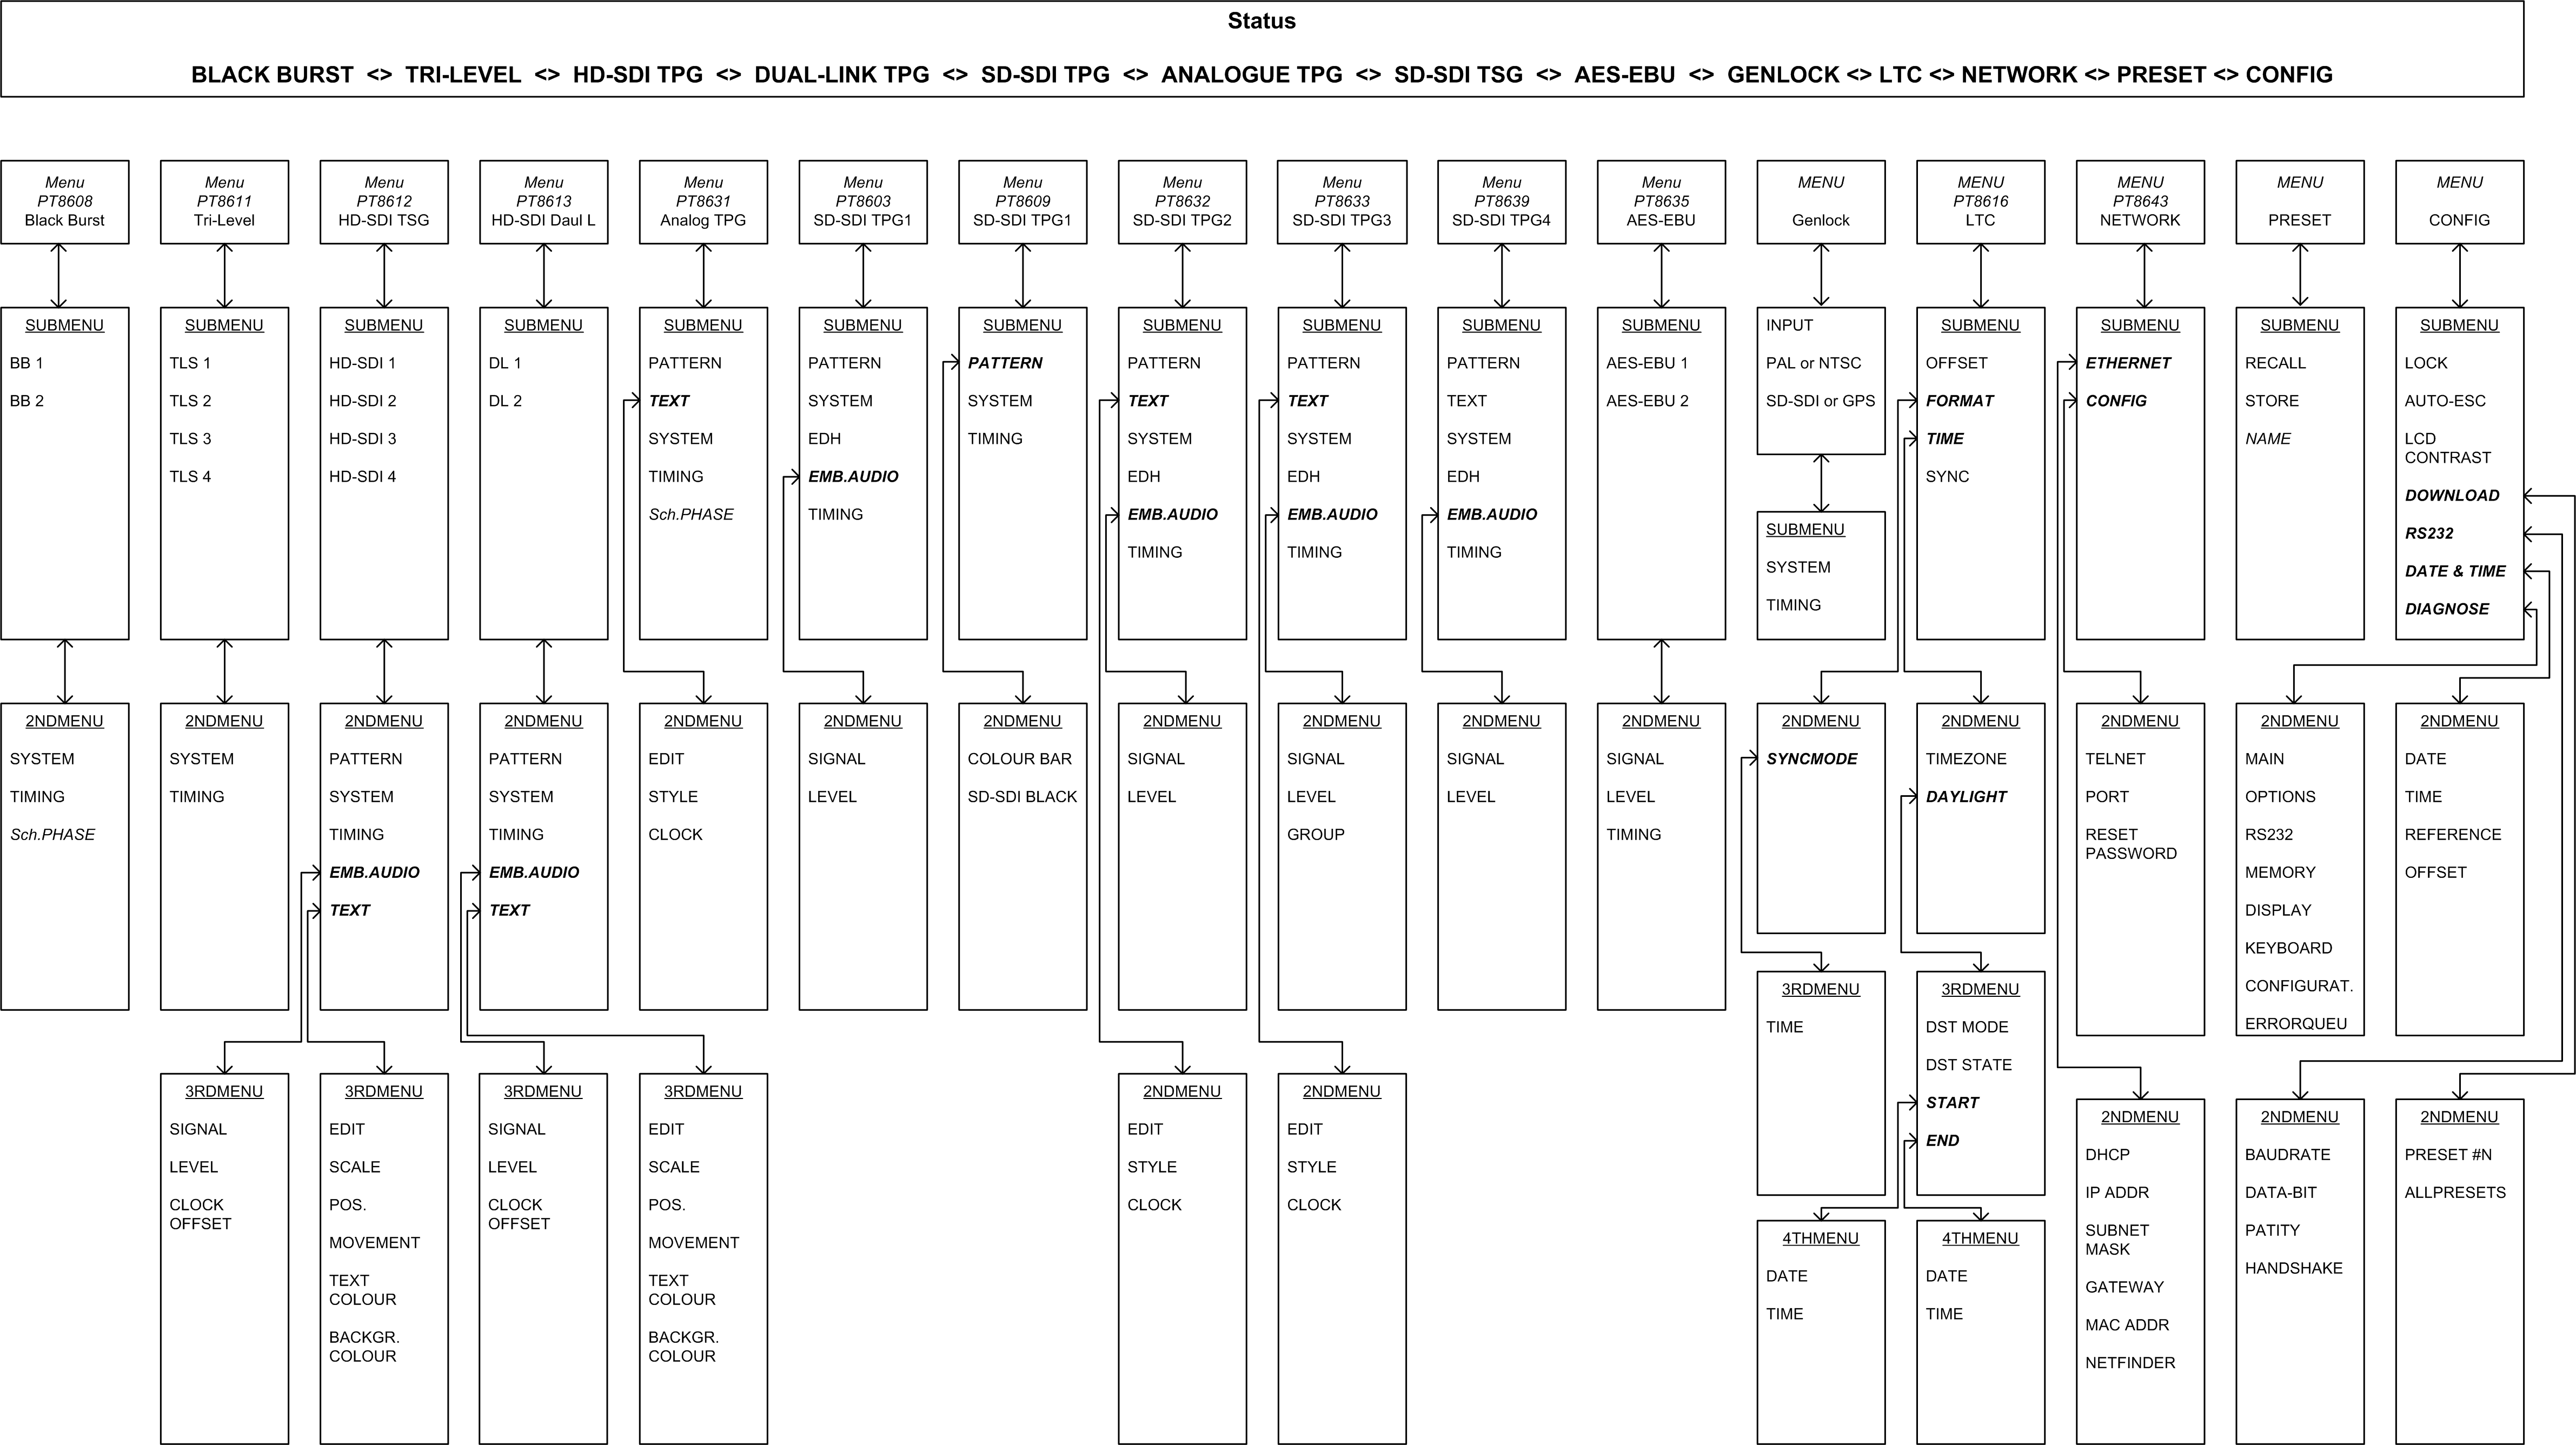
\includegraphics[width=0.75\textwidth]{fig/menu_tree}
	\caption{PT5300 Menu tree}
\end{figure}
\clearpage

\clearpage
\section{Remote Interface}
\label{cha:Remote}
\subsection{ General Information}

\textbf{Two remote interfaces are standard in the instrument:}

\begin{itemize}
\item A simple ground closure parallel interface, which allows remote control of some of the major operational parameters of the PT 5300
\item A serial remote gives control over all the functions of the PT 5300. The serial remoteoperates by use of an RS 232 communication port. 
\end{itemize}

To select type of remote interface move cable between connectors PAR (XM1) and SER (XR1) on Main Board (Unit 1).

\begin{figure}[hbt]
\centering
\includegraphics[width=0.5\textwidth]{fig/pt5300_overview}
\caption{Location of Connectors}
\end{figure}

\subsection{Parallel Remote}

The following parameters can be controlled when the remote connector is configured for parallel
ground closure control:
\begin{itemize}
\item Recall of preset \#1 to \#8
\item Selection of genlock mode
\end{itemize}

\subsubsection{Connector Description}

\textbf{Connector type:}
9 pin sub-D

\begin{figure}[hbt]
\centering
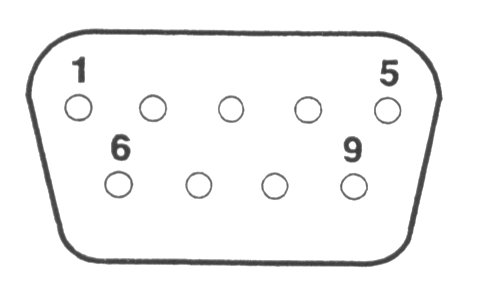
\includegraphics[width=0.5\textwidth]{fig/dsub}
\caption{Remote connector seen from rear panel}
\end{figure}

\begin{tabular*}{\textwidth}{@{\extracolsep{\fill}}|l|p{28em}|}
\hline
\textbf{Pin no.:} & \textbf{Function:} \\ \hline
1 & Preset 0 (LSB) \\ \hline
2 & Preset 1 \\ \hline
3 & Preset 2 (MSB) \\ \hline
4 & Genlock/Preset selection: \\
  & 0: Selects pin 6 active (pin 1-3 inactive) - genlock. \\ 
  & 1: Selects pin 1-3 active (pin 6 inactive) - preset. \\ \hline
5 & Ground \\ \hline
6 & Genlock selection: \\
  & 0: Selects external genlock (the result is unlocked if no valid signal is found in the active input). \\
  & 1: Selects internal reference. \\ \hline
7 & Genlock status output: \\
  & 0: Unlocked (using internal reference) \\
  & 1: Gen-locked or internal. \\ \hline
8 & Warning output: \\
  & 0: Error detected internal in the generator. \\
  & 1: No errors. \\ \hline
9 & Remote enable: \\
  & 0: Remote enabled. \\
  & 1: Remote disabled. \\ \hline
\end{tabular*}

\textbf{Note:} All outputs have internal pull up resistors to +5 V.

\textbf{Note:} The Presets are numbered binary. The binary number is one less than the number used in the menu system on the front of the generator.

\textbf{Note:} The remote output pins 7 and 8 are active even when the remote is disabled. The remote only has to be configured as parallel.

\textbf{Table of the selections:}

{\tiny
\begin{tabular}{|l|l|l|l|l|l|l|l|l|l|l|}
\hline
\textbf{Function:}		& \textbf{Pin 3} & \textbf{Pin 2} & \textbf{Pin 1} & \textbf{Pin 4} & \textbf{Pin 5} & \textbf{Pin 6} & \textbf{Pin 7} & \textbf{Pin 8} & \textbf{Pin 9} \\ \hline
 & \textbf{(MSB)} & \textbf{(LSB)} & & & & & & & \\ \hline
\textbf{Remote disabled} 	& X & X & X & X & GND & X & OUT & OUT & 1 \\ \hline
\textbf{Preset 1}					& 0 & 0 & 0 & 1 & GND & X & OUT & OUT & 0 \\ \hline
\textbf{Preset 2} 				& 0 & 0 & 1 & 1 & GND & X & OUT & OUT & 0 \\ \hline
\textbf{Preset 3}					& 0 & 1 & 0 & 1 & GND & X & OUT & OUT & 0 \\ \hline
\textbf{Preset 4}					& 0 & 1 & 1 & 1 & GND & X & OUT & OUT & 0 \\ \hline
\textbf{Preset 5}					& 1 & 0 & 0 & 1 & GND & X & OUT & OUT & 0 \\ \hline
\textbf{Preset 6}					& 1 & 0 & 1 & 1 & GND & X & OUT & OUT & 0 \\ \hline
\textbf{Preset 7}					& 1 & 1 & 0 & 1 & GND & X & OUT & OUT & 0 \\ \hline
\textbf{Preset 8}					& 1 & 1 & 1 & 1 & GND & X & OUT & OUT & 0 \\ \hline
\textbf{Genlock Int.}	& X & X & X & 0 & GND & 1 & OUT & OUT & 0 \\ \hline
\textbf{Genlock Ext.}	& X & X & X & 0 & GND & 0 & OUT & OUT & 0 \\ \hline
\end{tabular}
}

\subsection{Serial Remote}

The serial remote allows for control of virtually all functions in the generator as well as reading of instrument setting.
The serial remote operates electrically as an RS 232C communication port. %The parameter setting for the RS 232 communication port is described in xxx

\begin{figure}[hbt]
\centering
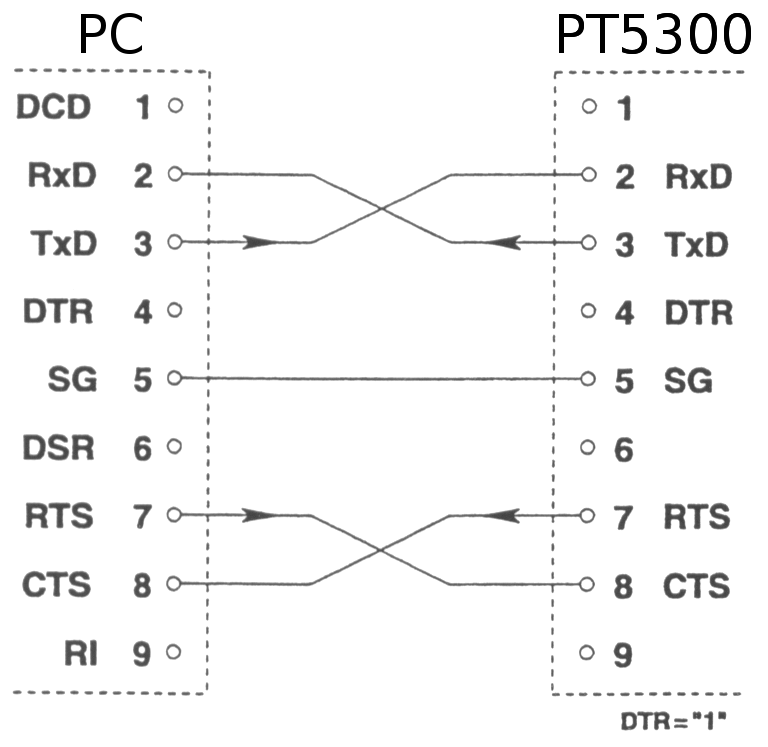
\includegraphics[width=0.5\textwidth]{fig/RS232_connection}
\caption{Configuration of cable between PC and PT 5300}
\end{figure}

The PT 5300 communication protocol complies with the:
\begin{itemize}
\item SCPI 1995.0: Standard Commands for Programmable Instruments, Vol I-IV. This protocol which is based on the IEEE 488.2 (IEEE Standard Codes, Formats, Protocols, and Common Commands). 
\end{itemize}

For the description of the commands a basic knowledge of operation of the instrument is assumed.

To use the serial remote a basic knowledge of the SCPI programming and computer control is also recommended. The paper: ``A beginner's Guide to SCPI'' by Barry Epler, Hewlett-Packard Press \copyright, 1991 can be used to gain the basic knowledge of the ideas behind the SCPI system.

\subsection{General Description of the Interface Syntax}

\subsubsection{General Information}
The remote system is organised in a tree structure. The structure defines sub-systems. In order to access command lower in the tree or in different branches the entire command string should be used. Indentation is used to indicate the root level and the branches. The highest level to the left. The complete command always includes all the root levels.

A space between a command string and an option is required, except in a query * where a space is not allowed.

Enter more than one command on a line by using a semicolon ``;'' as divider. A command line is terminated by $<$CR$> <$LF$>$. If the next command is part of the same command system the separation is a ``;'' only. If the next command is part of another command system the ``;'' is followed by a ``;''.

Parameters are separated from the header by a space. Several parameters are separated by a comma. 

Character strings should be placed in single or double quotation marks. 

The valid parameter ranges are shown in the command tables. Non valid values generate an error message.

\subsubsection{Syntax Elements}

\begin{tabular*}{\textwidth}{@{\extracolsep{\fill}}|l|p{28em}|}
; 		& Semicolon separates two commands of a command line and does not change the path.\\
: 		& Colon separates the keywords of a command. In a command line, a colon ``:'' after a separating semicolon ``;'' indicates the root control level.\\
, 		& Comma separates the parameter command.\\
? 		& Question mark identifies a query command (Query commands are formed by adding a question mark to the header).\\
* 		& Asterisk identifies a common command. (Common commands consists of a header preceded by an asterisk and possibly followed by one or more parameters)\\
' or '' & Single or double quote introduces and terminates a character string.\\
\# 		& Double dagger introduces block data. \\
Space & Space Character separates header and parameters.\\
$|$		& Parameters divided by a ``$|$'' indicates an ``or'' selection between the values shown. Only one value may be used at a time.\\
$[$xxxx$]$ & Square brackets indicate an optional specific string parameter used by some command systems.\\
XXXX 	& A vertical line through a command indicates a command not implemented. The command is included for future compatibility
reasons. The generator will not give any response to these command (error messages are not generated).\\
\end{tabular*}

\subsubsection{Command Syntax}

A command consists of a ``header'' and one or several ``parameters''. Header and parameters are separated by space. A header may consist of several keywords.

\subsubsection{Syntax of Program Messages}

A command or query is called a program message unit. Such a program message unit consists of a header, or a header separated by a space from one or more parameters. The program header separator between the header and the first parameter must be at least one ``whitespace'' character. The header consists of one or more mnemonics (key words) describing the command. The parameters in a message unit are also referred to as ``Data Elements''. They are mutually separated by a comma (,), which is referred to as ``Data Separator''. Furthermore the following rules are valid:

\begin{itemize}
\item Any one of the ``white space'' characters (dec. 0..9, 11.. 32) may:
\begin{itemize}
\item Precede a header
\item Precede the Message Terminator
\item Be placed in between the header and the parameter
\item Be placed in between two consecutive parameters
\item String data in a parameter must be specified between quotes. A quote may either be a
\end{itemize}
\item `single quote' (dec. 39) or a ``double quote'' character (dec. 34)
\end{itemize}

One or more program message units (commands) may be send within a single program message. Program message units are separated by a semicolon (;). A message of one or more units is terminated by a program message terminator.

The program message terminator must be the following code:
\begin{itemize}
\item LF <line feed> (dec.10) code
\end{itemize}

\textbf{Note:} Most controller programming languages send the terminator automatically, but allow it to be changed.

\textbf{Basically there are two types of program headers:}
\begin{itemize}
\item Compound headers - Commands have a compound header consisting of one of more key words (mnemonics), mutually separated by a colon (:) character. Such as a colon may also precede the header.
\item Command headers - The program messages that are standardised are called common commands. Their headers always start with an asterisk (*) character 
\end{itemize}

Each key word in a compound command header represents a node in the command tree. The left most key word is the root node, representing the highest hierarchical level in the command tree. Subsequent keyword represents sub nodes under the root node.

\subsubsection{Long and Short Form}

Program messages may be sent in either long or short form
\begin{itemize}
\item The long form is the full word
\item The short form is the first character of the long form
\end{itemize}

The short form in a syntax specification is shown in upper case, and the remaining part of the long form is shown in lower case characters.

\textbf{Note:} Upper and lower case, as used in syntax specification, is only a notation habit to facilitate distinction between long and short form. The generator itself does not differentiate between upper and lower case characters. In program messages, either the long or short form may be used in any mix of upper or lower case characters. There is no semantic difference between upper and lower case in program messages.

\subsubsection{Syntax of Response Messages}
The response to a query is a response message unit, consisting of one or more parameters (data elements). Successive parameters are separated by a comma (,). If there are multiple queries in a program message, the multiple response message units are grouped together in the corresponding response message. 

Response message units are separated by a semicolon (;) and are terminated by a response message terminator. 

The instrument will always send the response data in short form and in capitals. Headers are not sent in the response messages, parameters only.


\clearpage
\section{Command reference}
\label{cha:CommandRef}
\subsection{Reference Documents}

\begin{itemize}
\item IEEE 488.2-1987: IEEE Standard Codes, Formats, Protocols, and Common Commands
\item SCPI 1995.0: Standard Commands for Programmable Instruments, Vol I-IV.
\item ``A Beginner's Guide to SCPI'', Barry Epler, HEWLETT-PACKARD PRESS, 1991
\end{itemize}

\subsection{Configuration and Syntax}

\textbf{Control characters:}

\begin{tabular}{|l|l|}
\hline
Control character 	& Function \\ \hline
$<$Ctrl L$>$ 0x0C 	& Local lockout switchover. \\ 
										& Local lockout is \textbf{always} disabled after power-up \\ \hline
0x0A	 							& Terminator, i.e. newline $<$LF$>$ \\ \hline
\end{tabular}

\textbf{PT8604 Multiple parallel Black Burst:}


Multiple parallel Black Burst option is defined as BB2 when programming via RS232 except when requesting the version of the option. In this case a specific command exists.

%\textbf{Buffers}
%
%\begin{itemize}
%\item Receive buffer: 64 bytes
%\item Transmit buffer: 32 bytes
%\end{itemize}
%
%\textbf{Serial Port:}
%
%The 9-pin RS232 connector consists of:
%
%\begin{tabular}{|l|l|l|}
%\hline
%\textbf{Pin:} & \textbf{Name:} & \textbf{Description:} \\ \hline
%\textbf{1}		& DCD & Not used\\ \hline
%\textbf{2}		& RxD & Receiver pin\\ \hline
%\textbf{3}		& TxD & Transmitter pin\\ \hline
%\textbf{4}		& DTR & Not used\\ \hline
%\textbf{5}		& SG & Signal ground\\ \hline
%\textbf{6}		& DSR & Not used\\ \hline
%\textbf{7}		& RTS & Request to send\\ \hline
%\textbf{8}		& CTS & Clear to send\\ \hline
%\textbf{9}		& RI & Not used\\ \hline
%\end{tabular}

\subsection{Commands Summary}

All commands listed consist of both a set- and request-command unless specifically listed in the table as $<$query only$>$ or $<$no query$>$.

\begin{landscape}

\subsubsection{Mandated Commands}

\commandtable
*CLS	& - & & Clear Status Command \\ \hline
*ESE & & & \\ \hline
*ESE? & & & \\ \hline
*ESR? & & & \\ \hline
*IDN? & & & Device Identification Query \\ \hline
*OPC& & & \\ \hline
*OPC?& & & \\ \hline
*RST & & & Reset Command \\ \hline
*SRE& & & \\ \hline
*SRE?& & & \\ \hline
*STB?& & & \\ \hline
*TST?& & & \\ \hline
*WAI& & & \\ \hline
\end{longtable}



\subsubsection{Instrument Commands}

\textbf{DIAGnostic subsystem}

\commandtable
:DISPlay 		& - 					& 										& $<$no query$>$ \\ \hline
:ERRorqueue & 						& 										& 						\\ \hline
\hspace{1em}:RESet 	& - 	&	- 									&	$<$no query$>$ \\ \hline
:ERRorqueue & - 					&	- 									&	$<$query only$>$ \\ \hline
\end{longtable}

\textbf{DISPlay Subsystem}


\commandtable
:CONTrast & $<$0 to 20$>$ $|$ MIN $|$ MAX  & 16 & \\ \hline
\end{longtable}

\textbf{INPut Subsystem}


\commandtable
:GENLock 	& & & \\ \hline
\hspace{1em}:INPut		& A $|$ B $|$ A\_B $|$ SDI $|$ INTernal $|$ INTernal2 & A & \\ \hline
:SYSTem	& PALBurst $|$ NTScburst $|$ SYNC625 $|$ SYNC525 $|$ SDI625 $|$ SDI525 $|$ F358MHz $|$ F443MHz $|$ F5MHz $|$ F10MHz & \hspace{1em}PALBurst & \\ \hline
\hspace{1em}:DElay & $<$Field$>$,$<$Line$>$,$<$HTime$>$ & 0,0,0 & \\ \hline
:GENLock? & - & - & $<$query only$>$ \\ \hline
:SDIGenlock & & & \\ \hline
\hspace{1em}:VERSion? & - & & $<$query only$>$ \\ \hline
\end{longtable}

\textbf{OUTPut Subsystem}



\commandtable
:BB1 & & & \\ \hline
\hspace{1em}:SYSTem & PAL $|$ PAL\_ID $|$ NTSC & PAL & \\ \hline
\hspace{1em}:DELay & $<$Field$>$,$<$Line$>$,$<$HTime$>$ & 0,0,0 & \\ \hline
\hspace{1em}:SCHPhase & $<$179 to +180$>$ & 0 & \\ \hline
\hspace{1em}:VERSion? & - & - & $<$query only$>$ \\ \hline
:BB1? & - & - & $<$query only$>$ \\ \hline


& & & \\ \hline
:BB2 & & & \\ \hline
\hspace{1em}:SYSTem & PAL $|$ PAL\_ID $|$ NTSC & PAL & \\ \hline
\hspace{1em}:DELay & $<$Field$>$,$<$Line$>$,$<$HTime$>$ & 0,0,0 & \\ \hline
\hspace{1em}:SCHPhase & $<$179 to +180$>$ & 0 & \\ \hline
\hspace{1em}:VERSion? & - & - & $<$query only$>$ \\ \hline
:BB2? & - & - & $<$query only$>$ \\ \hline


& & & \\ \hline
:ATPGenerator2 & & & \\ \hline
\hspace{1em}:PATTerrn & $<$pattern\_name$>$ & CBEBu & \\ \hline
\hspace{1em}:MODify 	& OFF $|$ ON & & \\ \hline
\hspace{2em}:APAL 		& OFF $|$ ON & & \\ \hline
\hspace{2em}:PLUGe 		& OFF $|$ ON & & \\ \hline
\hspace{2em}:STAircase10	& OFF $|$ ON & & \\ \hline
\hspace{1em}:TEXT			&	& & \\ \hline
\hspace{2em}STRing1 	& OFF $|$ ON $<$string\_data$>$ & OFF,``ANALOG1'' OFF,``PTV'' & Standard Pattern Complex Pattern\\ \hline
\hspace{2em}STRing2		& OFF $|$ ON $<$string\_data$>$ & OFF,``ANALOG2'' OFF,``PT5230'' & Standard Pattern Complex Pattern\\ \hline
\hspace{2em}STRing3		& OFF $|$ ON $<$string\_data$>$ & OFF,``ANALOG3'' & Standard Pattern\\ \hline
\hspace{2em}STYLe			& STANdard $|$ COMPlex & COMPlex & \\ \hline 
\hspace{2em}CLOCk 		& OFF $|$ TIME $|$ DTIME & OFF & \\ \hline
\hspace{1em}:SYSTem 	& PAL $|$ PAL\_ID $|$ NTSC & PAL & \\ \hline
\hspace{1em}:DELay 		& $<$Field$>$,$<$Line$>$,$<$HTime$>$ & 0,0,0 & \\ \hline
\hspace{1em}:SCHPhase & $<$-179 to 180$>$ & 0 & \\ \hline
\hspace{1em}:VERSion?	& - & - & $<$query only$>$ \\ \hline
:ATPGenerator2? 			& - & - & $<$query only$>$ \\ \hline


& & & \\ \hline
:ATPGenerator5 & & & \\ \hline
\hspace{1em}:PATTerrn & $<$pattern\_name$>$ & CBEBu & \\ \hline
\hspace{1em}:MODify 	& OFF $|$ ON & & \\ \hline
\hspace{2em}:APAL 		& OFF $|$ ON & & \\ \hline
\hspace{2em}:PLUGe 		& OFF $|$ ON & & \\ \hline
\hspace{2em}:STAircase10	& OFF $|$ ON & & \\ \hline
\hspace{1em}:TEXT			&	& & \\ \hline
\hspace{2em}STRing1 	& OFF $|$ ON $<$string\_data$>$ & OFF,``ANALOG1'' OFF,``PTV'' & Standard Pattern Complex Pattern\\ \hline
\hspace{2em}STRing2		& OFF $|$ ON $<$string\_data$>$ & OFF,``ANALOG2'' OFF,``PT5230'' & Standard Pattern Complex Pattern\\ \hline
\hspace{2em}STRing3		& OFF $|$ ON $<$string\_data$>$ & OFF,``ANALOG3'' & Standard Pattern\\ \hline
\hspace{2em}STYLe			& STANdard $|$ COMPlex & COMPlex & \\ \hline 
\hspace{2em}CLOCk 		& OFF $|$ TIME $|$ DTIME & OFF & \\ \hline
\hspace{1em}:SYSTem 	& PAL $|$ PAL\_ID $|$ NTSC & PAL & \\ \hline
\hspace{1em}:DELay 		& $<$Field$>$,$<$Line$>$,$<$HTime$>$ & 0,0,0 & \\ \hline
\hspace{1em}:SCHPhase & $<$-179 to 180$>$ & 0 & \\ \hline
\hspace{1em}:VERSion?	& - & - & $<$query only$>$ \\ \hline
:ATPGenerator5? 			& - & - & $<$query only$>$ \\ \hline


& & & \\ \hline
:STSGenerator2 				&		&		& \\ \hline	
\hspace{1em}:PATTerrn & $<$pattern\_name$>$	& BLACk & 	\\ \hline
\hspace{1em}:SYSTem		& SDI525 $|$ SDI625		& SDI625 & \\ \hline
\hspace{1em}:DELay		& $<$Field$>$,$<$Line$>$,$<$HTime$>$ & 0,0,0 & \\ \hline
\hspace{1em}:EDHinsert& OFF $|$ ON &	OFF & \\ \hline
\hspace{1em}:EMBaudio & OFF $|$ SILence	& OFF & \\ \hline
\hspace{2em}:SIGNal 	& OFF $|$ S1KHZ 	& OFF & \\ \hline
\hspace{2em}:LEVel		& SILence $|$ DB0FS $|$ DB9FS $|$ DB15FS $|$ DB18FS & SILence & \\ \hline
\hspace{1em}:VERSion? & - & - & $<$query only$>$ \\ \hline
:STSGenerator2? 				& - & - & $<$query only$>$ \\ \hline


& & & \\ \hline
:STSGenerator3 				&		&		& \\ \hline	
\hspace{1em}:PATTerrn & $<$pattern\_name$>$	& BLACk & 	\\ \hline
\hspace{1em}:SYSTem		& SDI525 $|$ SDI625		& SDI625 & \\ \hline
\hspace{1em}:DELay		& $<$Field$>$,$<$Line$>$,$<$HTime$>$ & 0,0,0 & \\ \hline
\hspace{1em}:EDHinsert& OFF $|$ ON &	OFF & \\ \hline
\hspace{1em}:EMBaudio & OFF $|$ SILence	& OFF & \\ \hline
\hspace{2em}:SIGNal 	& OFF $|$ S1KHZ 	& OFF & \\ \hline
\hspace{2em}:LEVel		& SILence $|$ DB0FS $|$ DB9FS $|$ DB15FS $|$ DB18FS & SILence & \\ \hline
\hspace{1em}:VERSion? & - & - & $<$query only$>$ \\ \hline
:STSGenerator3 				& - & - & $<$query only$>$ \\ \hline


& & & \\ \hline
:STSGenerator4 				&		&		& \\ \hline	
\hspace{1em}:PATTerrn & $<$pattern\_name$>$	& BLACk & 	\\ \hline
\hspace{1em}:SYSTem		& SDI525 $|$ SDI625		& SDI625 & \\ \hline
\hspace{1em}:DELay		& $<$Field$>$,$<$Line$>$,$<$HTime$>$ & 0,0,0 & \\ \hline
\hspace{1em}:EDHinsert& OFF $|$ ON &	OFF & \\ \hline
\hspace{1em}:EMBaudio & OFF $|$ SILence	& OFF & \\ \hline
\hspace{2em}:SIGNal 	& OFF $|$ S1KHZ 	& OFF & \\ \hline
\hspace{2em}:LEVel		& SILence $|$ DB0FS $|$ DB9FS $|$ DB15FS $|$ DB18FS & SILence & \\ \hline
\hspace{1em}:VERSion? & - & - & $<$query only$>$ \\ \hline
:STSGenerator4 				& - & - & $<$query only$>$ \\ \hline


& & & \\ \hline
:STPGenerator1				&		&		& \\ \hline	
\hspace{1em}:PATTerrn	& $<$pattern\_name$>$ & CBEBu & \\ \hline
\hspace{1em}:MODify		& OFF $|$ ON & & \\ \hline
\hspace{2em}:APAL			& OFF $|$ ON & OFF & \\ \hline
\hspace{2em}:PLUGe		& OFF $|$ ON & OFF & \\ \hline
\hspace{2em}:STAircase10 &OFF $|$ ON & OFF & \\ \hline
\hspace{2em}MOTion		& OFF $|$ ON & OFF & \\ \hline
\hspace{1em}:TEXT			&	&	& \\ \hline
\hspace{2em}STRing1		& OFF $|$ ON $|$ $<$string\_data$>$ & OFF,``DIGITAL1'' OFF,``PTV'' & Standard Pattern Complex Pattern \\ \hline
\hspace{2em}STRing2		& OFF $|$ ON $|$ $<$string\_data$>$ & OFF,``DIGITAL2'' OFF,``PT5230'' & Standard Pattern Complex Pattern \\ \hline
\hspace{2em}STRing3		& OFF $|$ ON $|$ $<$string\_data$>$ & OFF,``DIGITAL3'' & Standard Pattern \\ \hline
\hspace{2em}STYLe			& STANdard $|$ COMPlex & COMPlex & \\ \hline
\hspace{2em}CLOCk			& OFF $|$ TIME $|$ DTIME & OFF & \\ \hline
\hspace{1em}:SYSTem		& SDI525 $|$ SDI625 & SDI625 & \\ \hline
\hspace{1em}:EDHinsert	& OFF $|$ ON	& OFF & \\ \hline
\hspace{1em}:EMBaudio	& OFF $|$ SILence & OFF & \\ \hline
\hspace{2em}:SIGNal		& OFF $|$ S800HZ $|$ S1KHZ $|$ SEBu1KHz $|$ SBBC1KHZ $|$ MEBU1KHZ $|$ M1KHZ $|$ DUAL & OFF & \\ \hline
\hspace{2em}:LEVel		& SILence $|$ DB0FS $|$ DB9FS $|$ DB12FS $|$ DB15FS $|$ DB16FS $|$ DB18FS $|$ DB20FS & SILence & \\ \hline
\hspace{1em}:DELay		& $<$Field$>$,$<$Line$>$,$<$HTime$>$ & 0,0,0 & \\ \hline
\hspace{1em}:VERSion? 	& - & - & $<$query only$>$ \\ \hline
:STPGenerator1?				& - & - & $<$query only$>$ \\ \hline


& & & \\ \hline
:STPGenerator2				&		&		& \\ \hline	
\hspace{1em}:PATTerrn	& $<$pattern\_name$>$ & CBEBu & \\ \hline
\hspace{1em}:MODify		& OFF $|$ ON & & \\ \hline
\hspace{2em}:APAL			& OFF $|$ ON & OFF & \\ \hline
\hspace{2em}:PLUGe		& OFF $|$ ON & OFF & \\ \hline
\hspace{2em}:STAircase10 &OFF $|$ ON & OFF & \\ \hline
\hspace{2em}MOTion		& OFF $|$ ON & OFF & \\ \hline
\hspace{1em}:TEXT			&	&	& \\ \hline
\hspace{2em}STRing1		& OFF $|$ ON $|$ $<$string\_data$>$ & OFF,``DIGITAL1'' OFF,``PTV'' & Standard Pattern Complex Pattern \\ \hline
\hspace{2em}STRing2		& OFF $|$ ON $|$ $<$string\_data$>$ & OFF,``DIGITAL2'' OFF,``PT5230'' & Standard Pattern Complex Pattern \\ \hline
\hspace{2em}STRing3		& OFF $|$ ON $|$ $<$string\_data$>$ & OFF,``DIGITAL3'' & Standard Pattern \\ \hline
\hspace{2em}STYLe			& STANdard $|$ COMPlex & COMPlex & \\ \hline
\hspace{2em}CLOCk			& OFF $|$ TIME $|$ DTIME & OFF & \\ \hline
\hspace{1em}:SYSTem		& SDI525 $|$ SDI625 & SDI625 & \\ \hline
\hspace{1em}:EDHinsert	& OFF $|$ ON	& OFF & \\ \hline
\hspace{1em}:EMBaudio	& OFF $|$ SILence & OFF & \\ \hline
\hspace{2em}:SIGNal		& OFF $|$ S800HZ $|$ S1KHZ $|$ SEBu1KHz $|$ SBBC1KHZ $|$ MEBU1KHZ $|$ M1KHZ $|$ DUAL & OFF & \\ \hline
\hspace{2em}:LEVel		& SILence $|$ DB0FS $|$ DB9FS $|$ DB12FS $|$ DB15FS $|$ DB16FS $|$ DB18FS $|$ DB20FS & SILence & \\ \hline
\hspace{1em}:DELay		& $<$Field$>$,$<$Line$>$,$<$HTime$>$ & 0,0,0 & \\ \hline
\hspace{1em}:VERSion? 	& - & - & $<$query only$>$ \\ \hline
:STPGenerator2?				& - & - & $<$query only$>$ \\ \hline


& & & \\ \hline
:STPGenerator5				&		&		& \\ \hline	
\hspace{1em}:PATTerrn	& $<$pattern\_name$>$ & CBEBu & \\ \hline
\hspace{1em}:MODify		& OFF $|$ ON & & \\ \hline
\hspace{2em}:APAL			& OFF $|$ ON & OFF & \\ \hline
\hspace{2em}:PLUGe		& OFF $|$ ON & OFF & \\ \hline
\hspace{2em}:STAircase10 &OFF $|$ ON & OFF & \\ \hline
\hspace{2em}MOTion		& OFF $|$ ON & OFF & \\ \hline
\hspace{1em}:TEXT			&	&	& \\ \hline
\hspace{2em}STRing1		& OFF $|$ ON $|$ $<$string\_data$>$ & OFF,``DIGITAL1'' OFF,``PTV'' & Standard Pattern Complex Pattern \\ \hline
\hspace{2em}STRing2		& OFF $|$ ON $|$ $<$string\_data$>$ & OFF,``DIGITAL2'' OFF,``PT5230'' & Standard Pattern Complex Pattern \\ \hline
\hspace{2em}STRing3		& OFF $|$ ON $|$ $<$string\_data$>$ & OFF,``DIGITAL3'' & Standard Pattern \\ \hline
\hspace{2em}STYLe			& STANdard $|$ COMPlex & COMPlex & \\ \hline
\hspace{2em}CLOCk			& OFF $|$ TIME $|$ DTIME & OFF & \\ \hline
\hspace{1em}:SYSTem		& SDI525 $|$ SDI625 & SDI625 & \\ \hline
\hspace{1em}:EDHinsert	& OFF $|$ ON	& OFF & \\ \hline
\hspace{1em}:EMBaudio	& OFF $|$ SILence & OFF & \\ \hline
\hspace{2em}:SIGNal		& OFF $|$ S800HZ $|$ S1KHZ $|$ SEBu1KHz $|$ SBBC1KHZ $|$ MEBU1KHZ $|$ M1KHZ $|$ DUAL & OFF & \\ \hline
\hspace{2em}:LEVel		& SILence $|$ DB0FS $|$ DB9FS $|$ DB12FS $|$ DB15FS $|$ DB16FS $|$ DB18FS $|$ DB20FS & SILence & \\ \hline
\hspace{1em}:DELay		& $<$Field$>$,$<$Line$>$,$<$HTime$>$ & 0,0,0 & \\ \hline
\hspace{1em}:VERSion? 	& - & - & $<$query only$>$ \\ \hline
:STPGenerator5?				& - & - & $<$query only$>$ \\ \hline


& & & \\ \hline
:AUDio1								&	&	&	\\ \hline
\hspace{1em}:SIGnal 	& S800Hz $|$ S1kHz $|$ SEBu1kHz $|$ SBBc1kHz $|$ MEBU1kHz $|$ M1kHz $|$ DUAL $|$ F48kHz $|$ WORDclock & S800Hz & \\ \hline
\hspace{1em}:LEVel 		& SILence $|$ DB0FS $|$ DB9FS $|$ DB12FS $|$ DB15FS $|$ DB16FS $|$ DB18FS $|$ DB20FS & SILence & \\ \hline
\hspace{1em}:TIMing 	& PAL $|$ NTSC1 $|$ NTSC2 $|$ NTSC3 $|$ NTSC4 $|$ NTSC5 & PAL & \\ \hline
\hspace{1em}:VERSion? & - & - & $<$query only$>$ \\ \hline
:AUDio1? 							& - & - & $<$query only$>$ \\ \hline


& & & \\ \hline
:AUDio2								&	&	&	\\ \hline
\hspace{1em}:SIGnal 	& S800Hz $|$ S1kHz $|$ SEBu1kHz $|$ SBBc1kHz $|$ MEBU1kHz $|$ M1kHz $|$ DUAL $|$ F48kHz $|$ WORDclock & S800Hz & \\ \hline
\hspace{1em}:LEVel 		& SILence $|$ DB0FS $|$ DB9FS $|$ DB12FS $|$ DB15FS $|$ DB16FS $|$ DB18FS $|$ DB20FS & SILence & \\ \hline
\hspace{1em}:TIMing 	& PAL $|$ NTSC1 $|$ NTSC2 $|$ NTSC3 $|$ NTSC4 $|$ NTSC5 & PAL & \\ \hline
\hspace{1em}:VERSion? & - & - & $<$query only$>$ \\ \hline
:AUDio2? 							& - & - & $<$query only$>$ \\ \hline


& & & \\ \hline
:TIMeclock						& & & \\ \hline
\hspace{1em}:DFORmat 	& DMY $|$ MDY $|$ YMD & DMY & \\ \hline
\hspace{1em}:DATe			& $<$year$>$,$<$month$>$,$<$date$>$ & 99,5,1 & \\ \hline
\hspace{1em}:TFORmat	& HOUR12 $|$ HOUR24 & HOUR24 & \\ \hline
\hspace{1em}:TIMe			& $<$hour$>$,$<$Minute$>$,$<$second$>$ & 8,0,0 & \\ \hline
\hspace{1em}:REFerence	& LTC $|$ VITC $|$ VFFRrequency $|$ REF1HZ $|$ INTernal & LTC & \\ \hline
\hspace{1em}:OFFSet		& $<$offset$>$ & 0 & \\ \hline
\hspace{1em}:VERSion?	& - & - & $<$query only$>$ \\ \hline
:TIMeclock?						& - & - & $<$query only$>$ \\ \hline


& & & \\ \hline
:TLG1-8								&	&	&	\\ \hline
\hspace{1em}:SYStem		& OFF $|$ HD1080P60 $|$ HD1080P5994 $|$ HD1080P50 $|$ HD1080I30 $|$ HD1080I2997 $|$ HD1080I25 $|$ HD1080P30 $|$ HD1080P2997 $|$ HD1080P25 $|$ HD1080P24 $|$ HD1080P2398 $|$ HD1080sF30 $|$ HD1080sF2997 $|$ HD1080sF25 $|$ HD1080sF24 $|$ HD1080sF2398 $|$ HD720P60 $|$ HD720P5994 $|$ HD720P50 $|$ HD720P30 $|$ HD720P2997 $|$ HD720P25 $|$ HD720P24 $|$ HD720P2398 & & \\ \hline
\hspace{1em}:DELay	&	$<$Field$>,<$Line$>,<$HTime$>$	&	&	\\ \hline
\hspace{1em}:VERSion?	& - & - & $<$query only$>$ \\ \hline
:HD1-8									&	&	&	\\ \hline
\hspace{1em}:PATTern	& BLACk $|$ SDICheck $|$ PLUGe $|$ LRAMp $|$ CLAPperbrd $|$ COLOrbar $|$ COMBInation $|$ WINdow $|$ CROSshatch $|$ WHITe	&	 &	\\ \hline
\hspace{2em}:MOD	& HH $|$ HS $|$ SS, A105 $|$ A100 $|$ A95 $|$ A90 $|$ A85 $|$ A80 $|$ A75 $|$ A70 $|$ A65 $|$ A60 $|$ A55 $|$ A50 $|$ A45 $|$ A40 $|$ A35 $|$ A30 $|$ A25 $|$ A20 $|$ A15 $|$ A10 $|$ A5 $|$ A0 $|$ AM5 & & Applies only for certain patterns \\ \hline
\hspace{1em}:SYStem		& OFF $|$ HD1080I30 $|$ HD1080I2997 $|$ HD1080I25 $|$ HD1080P30 $|$ HD1080P2997 $|$ HD1080P25 $|$ HD1080P24 $|$ HD1080P2398 $|$ HD720P60 $|$ HD720P5994 $|$ HD720P50 $|$ HD720P30 $|$ HD720P2997 $|$ HD720P25 $|$ HD720P24 $|$ HD720P2398 $|$ SD525 $|$ SD625 & & \\ \hline
\hspace{1em}:EMBaudio	&	&	& \\ \hline
\hspace{2em}:SIGnal	&	SILence $|$ SINE $|$ CLICK $|$ OFF & & \\ \hline
\hspace{2em}:LEVel	&	DB0FS $|$ DB6FS $|$ DB12FS $|$ DB18FS $|$ DB24FS & & \\ \hline
\hspace{2em}:CLIck	&	-499 to 500	&	& \\ \hline
\hspace{1em}:TEXT		&	&	&	\\ \hline
\hspace{2em}:STRing1	&	``TEXT1'' &	&	\\ \hline
\hspace{2em}:STRing2	&	``TEXT2'' &	&	\\ \hline
\hspace{2em}:STRing3	&	``TEXT3'' &	&	\\ \hline
\hspace{2em}:MOVement	&	OFF $|$ VERtical $|$ HORizontal $|$ BOTH	&	&	\\ \hline
\hspace{2em}:SCAle	& 1 to 4	&	&	\\ \hline
\hspace{2em}:COLor	& WHIte $|$ YELlow $|$ CYAn $|$ GREen $|$ MAGenta $|$ BLUe $|$ BLAck &	& \\ \hline
\hspace{2em}:BACKground & WHIte $|$ YELlow $|$ CYAn $|$ GREen $|$ MAGenta $|$ BLUe $|$ BLAck &	& \\ \hline
\hspace{1em}:DELay	&	$<$Field$>,<$Line$>,<$HTime$>$	&	&	\\ \hline
\hspace{1em}:VERSion?	& - & - & $<$query only$>$ \\ \hline
:VERSion? 	& - & - & $<$query only$>$ \\ \hline


& & & \\ \hline
:DL1-4									&	&	&	\\ \hline
\hspace{1em}:PATTern	& BLACk $|$ SDICheck $|$ PLUGe $|$ LRAMp $|$ CLAPperbrd $|$ COLOrbar $|$ COMBInation $|$ WINdow $|$ CROSshatch $|$ WHITe	&	 &	\\ \hline
\hspace{2em}:MOD	& HH $|$ HS $|$ SS, A105 $|$ A100 $|$ A95 $|$ A90 $|$ A85 $|$ A80 $|$ A75 $|$ A70 $|$ A65 $|$ A60 $|$ A55 $|$ A50 $|$ A45 $|$ A40 $|$ A35 $|$ A30 $|$ A25 $|$ A20 $|$ A15 $|$ A10 $|$ A5 $|$ A0 $|$ AM5 & & Applies only for certain patterns \\ \hline
\hspace{1em}:SYStem		& OFF $|$ HD1080I30 $|$ HD1080I2997 $|$ HD1080I25 $|$ HD1080P30 $|$ HD1080P2997 $|$ HD1080P25 $|$ HD1080P24 $|$ HD1080P2398 $|$ HD1080sF30 $|$ HD1080sF2997 $|$ HD1080sF25 $|$ HD1080sF24 $|$ HD1080sF2398 $|$ HD720P60 $|$ HD720P5994 $|$ HD720P50 $|$ HD720P30 $|$ HD720P2997 $|$ HD720P25 $|$ HD720P24 $|$ HD720P2398 $|$ SD525 $|$ SD625 & & \\ \hline
\hspace{2em}:INTERFace	&	I1 $|$ I2 $|$ I3 $|$ I4 $|$ I5 $|$ I6 &	&	\\ \hline
\hspace{1em}:EMBaudio	&	&	& \\ \hline
\hspace{2em}:SIGnal	&	SILence $|$ SINE $|$ CLICK $|$ OFF & & \\ \hline
\hspace{2em}:LEVel	&	DB0FS $|$ DB6FS $|$ DB12FS $|$ DB18FS $|$ DB24FS & & \\ \hline
\hspace{2em}:CLIck	&	-499 to 500	&	& \\ \hline
\hspace{1em}:TEXT		&	&	&	\\ \hline
\hspace{2em}:STRing1	&	``TEXT1'' &	&	\\ \hline
\hspace{2em}:STRing2	&	``TEXT2'' &	&	\\ \hline
\hspace{2em}:STRing3	&	``TEXT3'' &	&	\\ \hline
\hspace{2em}:MOVement	&	OFF $|$ VERtical $|$ HORizontal $|$ BOTH	&	&	\\ \hline
\hspace{2em}:SCAle	& 1 to 4	&	&	\\ \hline
\hspace{2em}:COLor	& WHIte $|$ YELlow $|$ CYAn $|$ GREen $|$ MAGenta $|$ BLUe $|$ BLAck &	& \\ \hline
\hspace{2em}:BACKground & WHIte $|$ YELlow $|$ CYAn $|$ GREen $|$ MAGenta $|$ BLUe $|$ BLAck &	& \\ \hline
\hspace{1em}:DELay	&	$<$Field$>,<$Line$>,<$HTime$>$	&	&	\\ \hline
\hspace{1em}:VERSion?	& - & - & $<$query only$>$ \\ \hline


& & & \\ \hline
:LTCGenerator1-2	&	& & \\ \hline
\hspace{1em}:FORMat	&	$<$Format$>$,$<$Syncmode$>$,$<$Hour$>$,$<$Min$>$ & & 
							24FPS $|$ 25FPS $|$ 2997NOND $|$ 2997DROP $|$ 30FPS, NONE $|$ CONF $|$ AUTO, 0..23, 0..59  \\ \hline
\hspace{1em}:OFFSET & -5000000..4999999 & & \\ \hline
\hspace{1em}:TIMEZone	& $<$Hour$>$, $<$Min$>$ & & -11..+11, 0 $|$ 30 \\ \hline
\hspace{1em}:DAYLight & & & \\ \hline
\hspace{2em}:MODE & $<$Mode$>$, $<$State$>$ & & AUTO $|$ CONF $|$ AUTO, ON $|$ OFF \\ \hline
\hspace{2em}:START & $<$Month$>$, $<$Day$>$, $<$Hour$>$ & & 1..12, 1..31, 0..23 \\ \hline
\hspace{2em}:END & $<$Month$>$, $<$Day$>$, $<$Hour$>$ & & 1..12, 1..31, 0..23 \\ \hline


\end{longtable}


\end{landscape}

\subsection{Commands Explanation}

\subsubsection{Mandated Commands}

\textbf{*CLS CLEAR STATUS}\\
Clear the error queue. Reset of the event registers has NOT been implemented in this version.

\textbf{*ESE STANDARD EVENT STATUS ENABLE COMMAND}\\
The device accepts this command but does not respond to it.

\textbf{*ESE? STANDARD EVENT STATUS ENABLE QUERY}\\
The device accepts this command but does not respond to it.

\textbf{*ESR? STANDARD EVENT STATUS REGISTER QUERY}\\
The device accepts this command but does not respond to it.

\textbf{*IDN? IDENTIFICATION QUERY}\\
The response contains four fields:
\begin{itemize}
\item Field 1: Company name
\item Field 2: Product name
\item Field 3: Serial number (KUxxxxxxx)
\item Field 4: Firmware level, i.e. software revisions for Mainboard-OSC
\end{itemize}

Example:
\textit{*IDN? response: PTV,PT5230,KU123456,1.0-1.2}

\textbf{*OPC OPERATION COMPLETE}\\
The device accepts this command but does not respond to it.

\textbf{*OPC? OPERATION COMPLETE QUERY}\\
The device accepts this command but does not respond to it.

\textbf{*RST RESET}\\
Resets the device to factory preset status. The six presets are NOT reset, i.e. any user preset will NOT be erased. The internal errorqueue and the SCPI errorqueue will also be reset. Finally the device and any optional units will be reset.

\textbf{*SRE SERVICE REQUEST ENABLE}\\
The device accepts this command but does not respond to it.

\textbf{*SRE? SERVICE REQUEST ENABLE QUERY}\\
The device accepts this command but does not respond to it.

\textbf{*STB? READ STATUS BYTE QUERY}\\
The device accepts this command but does not respond to it.

\textbf{*TST? SELF-TEST QUERY}\\
The device accepts this command but does not respond to it.

\textbf{*WAI WAIT TO CONTINUE}\\
The device accepts this command but does not respond to it.

\subsubsection{Required Commands}

\textbf{SYSTem commands}

\textbf{SYSTem:ERRor?}\\
Command for reading an SCPI error message from the error queue. See Chapter \ref{cha:error_codes} for a complete list of error codes.

Example:\\
\textit{SYST:ERR? response: -102,``Syntax error''}

\textbf{SYSTem:VERSion?}\\
Command for reading the SCPI version to which the RS232 implementation complies.

Example:\\
\textit{SYST:VERS? response: 1995.0}

\textbf{SYSTem:PRESet[:RECall]}\\
Command to recall a stored generator configuration from a preset. Six user presets from 1 to 6 are available.

Example:\\
\textit{SYST:PRES:REC 3}\\
recall preset 3 in the generator

\textit{SYST:PRES:REC?}\\
response: 3, i.e. preset 3 is currently active

\textbf{SYSTem:PRESet:STORe}\\
Command to store the actual configuration in a preset. Six user presets from 1 to 6 are available.

Example:\\
\textit{SYST:PRES:STOR 6}\\
store configuration in preset 6

\textbf{SYSTem:PRESet:NAMe}\\
Command for naming a user preset. Six user presets from 1 to 6 are available. Number of characters in the name are limited to sixteen, 16.

Example:\\
\textit{SYST:PRES:NAME 2,``WHAT'''}\\
name preset number 2 ``WHAT'

\textit{SYST:PRES:NAME? 2}\\
response: ``WHAT''

\textbf{SYSTem:PRESet:DOWNload}\\
Command for downloading, i.e. reading a complete preset from a PT5300 . Six user presets from 1 to 6 are available.\NoTelnetSupport

Example:\\
\textit{SYST:PRES:DOWN 4}\\
download content of preset 4

\textbf{SYSTem:PRESet:UPLoad}\\
Command for downloading, i.e. reading a complete preset from a PT5300 . Six user presets from 1 to 6 are available.\NoTelnetSupport

Example:\\
\textit{SYST:PRES:UP 4, \#aaa\ldots}\\
upload block data aaa to preset 4

\textbf{SYSTem:DOWNload}\\
Command for downloading, i.e. reading a complete PT5300 configuration incl. all presets.\NoTelnetSupport

Example:\\
\textit{SYST:DOWN}\\
download the complete PT5300

\textbf{SYSTem:UPLoad}\\
Command for uploading, i.e. storing a complete PT5300 configuration incl. all presets.\NoTelnetSupport
Example:\\
\textit{SYST:UP \#aaa\ldots}\\
upload block data aaa to PT5300

\textbf{STATus commands}

\textbf{STATus:OPERaction[:EVENT]?}\\
The device accepts this command but does not respond to it.

\textbf{STATus:OPERation:CONDition?}\\
The device accepts this command but does not respond to it.

\textbf{STATus:OPERation:ENABle}\\
The device accepts this command but does not respond to it.

\textbf{STATus:QUEStionable[:EVENt]?}\\
The device accepts this command but does not respond to it.

\textbf{STATus: QUEStionable:CONDition?}\\
The device accepts this command but does not respond to it.

\textbf{STATus: QUEStionable:ENABle}\\
The device accepts this command but does not respond to it.

\textbf{STATus:PT5300?}\\
Command to read the internal error status of the generator. If errors are detected use the command:

\textbf{DIAGnostic:ERRorqueue?}\\
to read the specific error. 

Response Description:

\begin{tabular}{|p{10em}|p{22em}|}
\hline
``No errors'' 			& No errors have occurred after power up. \\ \hline
``Active error''		& The generator presently has an error. \\ \hline
``No active error''	& The generator presently has no error, but one or more errors have been detected after power up. \\
\hline
\end{tabular}

Example:\\
\textit{STAT:PT5300?}\\
response: ``No active error''

\subsubsection{Instrument Commands}

\textbf{DIAGnostic commands}

\textbf{DIAGnostic:DISPlay}\\
The device accepts this command but does not respond to it.

\textbf{DIAGnostic:ERRorqueue:RESet}\\
Command to reset the internal error queue of the generator. The errorqueue is a circular queue consisting of five entries.

Example:\\
\textit{DIAG:ERR:RES}\\
reset the five elements in the errorqueue

\textbf{DIAGnostic:ERRorqueue?}\\
Command to read an entry in the errorqueue and point to next entry in the errorqueue. This command should be executed five times to read the complete errorqueue.

Example:\\
\textit{DIAG:ERR?}\\
response: -108,``Parameter not allowed''

\textbf{DISPlay commands}

\textbf{DISPlay:CONTrast}\\
The device accepts this command but does not respond to it.

\textbf{INPut commands}

\textbf{INPut:GENLock:INPut}\\
Command for selecting the genlock input. Possible selections are 

\begin{tabular}{|l|l|}
\hline
\textbf{Input:} & \textbf{Description:} \\ \hline
A & A \\ \hline
B & B \\ \hline
A\_B & A-B, i.e. loop through \\ \hline
SDI & SDI Genlock, (ONLY available with option PT 8606)\\ \hline
INTernal & Internal\\ 
\hline
\end{tabular}

When selecting a new input, the system for that particular input will apply.

Example:\\
\textit{INP:GENL:INP A\_B}\\
select input A/B as the genlock signal\\
\textit{INP:GENL:INP?}\\
response: A\_B

\textbf{INPut:GENLock:SYSTem}\\
Command for selecting the genlock system. Possible selections are 

%\begin{center}
\begin{tabular}{|l|l|l|l|}
\hline
\textbf{System:} 	& \textbf{A, B\& A\_B} & \textbf{SDI:} & \textbf{Description:} \\
PALBurst					& X 									&								&	PAL burst lock 		\\ \hline
NTSCburst					& X 									&								& NTSC burst lock		\\ \hline
SYNC625						& X										& 							& 625 sync lock			\\ \hline
SYNC525						& X										&								& 525 sync lock			\\ \hline
SDI625						&											& X							& 625/50 lock				\\ \hline
SDI525						&											& X							& 525/59.95 lock		\\ \hline
F358MHz						& X										&								& 3.58 MHz lock			\\ \hline
F443MHz						& X										& 							& 4.43 MHz lock			\\ \hline
F5MHz							& X										&								& 5 MHz lock				\\ \hline
F10MHz						& X										&								& 10 MHz lock				\\ \hline
\end{tabular}
%\end{center}

\textbf{Note:} When the input has been selected as Internal or Internal2, issuing this command will result in an error, namely: -200, ``Execution error''. This error will also occur if selecting a system which is invalid for the active input.

Example:\\
\textit{INP:GENL:SYST F358MHz}\\
set system to 3.59 MHz clock\\
\textit{INP:GENL:SYST?}\\
response: F358 MHz

\textbf{INPut:GENLock:DELay}
Command to set the delay for the genlock input. The delay is defined by three parameters $<$Field$>$,$<$Line$>$,$<$HTime$>$
where $<$Field$>$ sets the field offset, $<$Line$>$ sets the line offset and $<$HTime$>$ sets the horizontal time in ns, i.e.

\begin{itemize}
\item HTime(PAL$<$64000.0ns 
\item HTime(NTSC)$<$63492.1ns
\end{itemize}

\textbf{Note:} It is not possible to select timing when the genlock system is 3.58 MHz, 4,43 MHz, 5 MHz, or 10 MHz or the input is set to internal or internal2. This will result in an execution error, namely: -200,``Execution error''. 

Also it is not possible to select a delay outside the range of the selected system. See table below:

%\begin{tabular}{|p{4em}|p{4em}|p{4em}|p{4em}|p{4em}|p{4em}|p{4em}|p{4em}|}
\begin{tabular}{|l|l|l|l|l|l|l|l|}
\hline
\multicolumn{4}{|c|}{Analogue} & \multicolumn{4}{|c|}{Digital} \\ 
\hline
\multicolumn{2}{|c|}{PAL, 625 Lines} & \multicolumn{2}{|c|}{NTSC, 625 Lines} & \multicolumn{2}{|c|}{D1, 625 Lines} & \multicolumn{2}{|c|}{D1, 525 Lines} \\ 
\hline
Field: 	& Line: 			& Field: 				& Line: 			& Field:	& Line:			 	& Filed: 	& Line: \\ \hline
-3 			& -0,..,-312	& -							& -						& -				& -						& -				& - \\ \hline
-2			& -0,..,-311	& -							& -						& -				& -						& -				& - \\ \hline
-1			& -0,..,-312	& -1 						& -0,..,-262	& -				& -						& -				& -  \\ \hline
-0			& -0,..,+311	& -0 						& -0,..,-261	& -0			& -0,..,-312	& -0			& -0,..,-262 \\ \hline
+0			& +0,..,+312	& +0						& -0,..,+262	& +0			& +0,..,+311	& +0			&	-0,..,+261 \\ \hline
+1			& +0..,+311		& +1						& -0,..,+261	& +1			& +0					& +1			& +0  \\ \hline
+2			& +0..,+312		& +2						& +0					& -				& -						& -				& - \\ \hline
+3			& +0..,+311		& -							& -						& -				& -						& -				& - \\ \hline
+4			& +0					& -							& -						& -				& -						& -				& - \\ \hline
\end{tabular}

Example:\\
\textit{INP:GENL:DEL+2,+5,+123.5}\\
set delay to 2 field, 5 line \& 123,5 ns\\
\textit{INP:GENL:DEL?}\\
response: +2,+005,+00123.5

\textbf{INPut:GENLock?}\\
Command to display the status and the settings of the genlock. The respond is defined as:
$<$lock info$>$,$<$input$>$,$<$system$>$,$<$Field$>$,$<$Line$>$,$<$HTime$>$ where $<$lock info$>$ is either GENLOCKED or UNLOCKED. 

For an explanation concerning the rest of the response see the commands: 

INP:GENL:INP, INP:GENL:SYST and INP:GENL:DEL.

\textbf{Note:} The response will always return the above six parameters. But when selecting the input as INTERNAL the parameters $<$system$>$,$<$Field$>$,$<$Line$>$,$<$HTime$>$ will have no meaning. Also when selecting the system as a timing, e.g. 3.58 MHz, the parameters $<$Field$>$,$<$Line$>$,$<$HTime$>$ will have no meaning. In these cases the returned values should be discarded and only the relevant parameters should be used.

Example:\\
\textit{INP:GENL?}\\
response: UNLOCKED,A,NTSCBURST,+1,212,00000.2\\
\textit{INP:GENL?}\\
response: UNLOCKED,A,F358 MHz,+0,+0,+0\\
\textit{INP:GENL?}\\
response: UNLOCKED,INTERNAL,NA, +0,+0,+0

\textbf{INPut:SDIGenlock:VERSion?}\\
Command to display the version of the optional PT 8606 SDI Genlock. The response contains four fields:
\begin{itemize}
\item Field 1: Company name
\item Field 2: Type name
\item Field 3: Serial number (KU number)
\item Field 4: Not available for this option, i.e. the returned value is 0.
\end{itemize}

Example:\\
\textit{INP:SDIG:VERS?}\\
Response: PTV,PT 8606,KU123456,0

\textbf{OUTPut commands}

\textbf{OUTPut:BB1:SYSTem}\\
\textbf{OUTPut:BB2:SYSTem}\\
Command to select the system of the standard Black Burst module. Systems available are:

\begin{tabular}{|l|l|}
\hline
\textbf{System:} & \textbf{Description:} \\ \hline
PAL & PAL \\ \hline
PAL\_ID & PAL with line 7 pulse \\ \hline
NTSC & NTSC with setup \\ 
\hline
\end{tabular}

Example:\\
\textit{OUTP:BB1:SYSTPAL\_ID}\\
set system for BB module 1 to PAL with line 7 pulse\\
\textit{OUTP:BB1:SYST?}\\ 
response: PAL\_ID

\textbf{OUTPut:BB1:DELay}\\
\textbf{OUTPut:BB2:DELay}\\
Command to set the delay of the standard Black Burst module. The delay is defined by three parameters: $<$Field$>$,$<$Line$>$,$<$HTime$>$
where $<$Field$>$ sets the field offset, $<$Line$>$ sets the line offset and $<$HTime$>$ sets the horizontal time in ns, i.e.
\begin{itemize}
\item HTime(PAL)$<$64000.0ns
\item HTime(NTSC)$<$63492.1ns
\end{itemize}

\textbf{Note:} It is not possible to select a delay outside the range of the selected system. See table below:

\begin{tabular}{|l|l|l|l|}
\hline
\multicolumn{4}{|c|}{Analogue} \\ 
\hline
\multicolumn{2}{|c|}{PAL, 625 Lines} & \multicolumn{2}{|c|}{NTSC, 625 Lines} \\ 
\hline
Field: 	& Line: 			& Field: 				& Line: 			\\ \hline
-3 			& -0,..,-312	& -							& -						\\ \hline
-2			& -0,..,-311	& -							& -						\\ \hline
-1			& -0,..,-312	& -1 						& -0,..,-262	\\ \hline
-0			& -0,..,+311	& -0 						& -0,..,-261	\\ \hline
+0			& +0,..,+312	& +0						& -0,..,+262	\\ \hline
+1			& +0..,+311		& +1						& -0,..,+261	\\ \hline
+2			& +0..,+312		& +2						& +0					\\ \hline
+3			& +0..,+311		& -							& -						\\ \hline
+4			& +0					& -							& -						\\ \hline
\end{tabular}

Example:\\
\textit{OUTP:BB2:DEL-0,-0,-3245.2}\\
set delay for BB module 2 to -2 field, -4 line \& -3245.2ns\\
\textit{OUTP:BB2:DEL?}\\
response: -2,-004,-03245.2\\

\textbf{OUTPut:BB1:SCHPhase}\\
\textbf{OUTPut:BB2:SCHPhase}\\
Command to set the ScH-Phase of the standard Black Burst module. The ScH-Phase value must be in the range: -179$<$ScH-Phase$<$=+180

Example:\\
\textit{OUTP:BB2:SCHP-160}\\
set the ScHPhase for BB module 2 to -160deg\\
\textit{OUTP:BB2:SCHP?}\\
response: -160

\textbf{OUTPut:BB1:VERSion?}\\
\textbf{OUTPut:BB2:VERSion?}\\
Command to display the version of the standard Black Burst module. The response contains four fields:
\begin{itemize}
\item Field 1: Company name
\item Field 2: Type name, which in this case is NA, not available
\item Field 3: Serial number (KUxxxxxx)
\item Field 4: Software version for the Black Burst module
\end{itemize}

\textbf{Note:} The response from this command is identical for both BB module 1 and 2. 

Example:\\
\textit{OUTP:BB1:VERS?}\\
response: PTV,NA,KU123456,2.1

\textbf{OUTPut:BB1?}\\
\textbf{OUTPut:BB2?}\\
Command to display the complete settings of the standard Black Burst modules. The response contains five fields: $<$System$>$,$<$Field$>$,$<$Line$>$,$<$HTime$>$,$<$ScHPhase$>$

For an explanation of the response, see the commands: 

OUTP:BBn:SYST,OUTP:BBn:DEL and OUTP:BBn:SCHP, where n:1 or 2

Example:\\
\textit{OUTP:BB1?}\\
response: PAL,+2+123,+12345.5,-160

\textbf{OUTPUT:ATPGenerator2:PATTern}\\
\textbf{OUTPUT:ATPGenerator5:PATTern}\\
Command to select the pattern of an optional PT 8631 Analog Test Pattern Generator. Patterns available are:

\begin{tabular}{|l|l|l|l|}
\hline
\textbf{Pattern:}	& \textbf{PAL:}	& \textbf{NTSC:}	& \textbf{Description:} \\ \hline
CBSMpte		& 			&	X			& SMPTE Colour Bar \\ \hline
CBEBu			& X			& 			& EBU Colour Bar \\ \hline
CBFCc			&				& X			& FCC Colour Bar \\ \hline
CB100			& X			& 			& 100\% Colour Bar \\ \hline
CBGRey75	& X			&				& Split field Colour bar w/75\% grey \\ \hline
CBRed75		& X			&				& Split field Colourbar w/75\% red \\ \hline
RED75			& X			& X			& 75\% Red \\ \hline
LSWeep		& X			& X			& Luminance sweep \\ \hline
MPULse		& X			& X			& Multipulse \\ \hline
SINXx			& X			& X			& Sinx/x \\ \hline
CCIR18		& X			&				& CCIR line 18 \\ \hline
NCMB			& 			& X			& NTC7 Combination \\ \hline
FCCMburst	& 			& X			& FCC Multiburst \\ \hline
WIN15			& X 		& X			& Window 15\% \\ \hline
WIN20			& X			& X			& Window 20\% \\ \hline
WIN100		& X			& X			& Window 100\% \\ \hline
GREy50		& X			& X			& Grey 50\% \\ \hline
WHITe100	& X			& X			& White 100\% \\ \hline
BLACkburst& X			& X			& Black Burst \\ \hline
FSWave		& X			& X			& Field square wave \\ \hline
BLWH01		& X			& X			& 0.1Hz Black/white \\ \hline
RAMP			& X			& X			& Ramp \\ \hline
MRAMp			& X			& X 		& Ramp Modulated \\ \hline
STAircase5& X			& X			& Staircase 5 step \\ \hline
MSTaircase5& X		& X			& Staircase 5 step modulated \\ \hline
STAircase10& X		& X			& Staircase 10 step \\ \hline
PBAR			& X			& X			& Pulse \& Bar \\ \hline
CCIR17		& X 		& 			& CCIR line 17\\ \hline
CCIR330		& X			&				& CCIR line 330\\ \hline
CCIR331		& X			&				& CCIR line 331\\ \hline
FCCComposite	&		& X			& FCC Composite\\ \hline
NCMP			&				& X			& NTC7 Composite\\ \hline
PHILips43	& X			&				& Philips pattern 4:3 format\\ \hline
PHILips169	& X		&				& Philips pattern 16:9 format\\ \hline
FUBK43		&	X			&				& FuBK pattern 4:3 format\\ \hline
FUBK169		& X			&				& FuBK pattern 16:9 format\\ \hline
CROSshatch	& X		& X			& Cross Hatch\\ \hline
CROSshatch169	& X	& X			& Cross Hatch in 16:9\\ \hline
CIRCl43		& X			&				& White circle on black in 4:3\\ \hline
CIRCl169	& X			& 			&	White circle on black in 16:9\\ \hline
PLUGe			& X			& X			& Pluge\\ \hline
SAFerea		& X			& X			& Safe area\\ \hline
SWAVe250	& X			& X			& Squarewave 250kHz\\ \hline
VMT01			& X			&				& VMT01 testpattern\\ \hline
\end{tabular}

\textbf{Note:} Not all the patterns are available in both systems. Trying to select a pattern not available in the active system will result in an error, namely: -200, ``Execution error''.

Example:\\
\textit{OUTP:ATPG2:PATT PHIL43}\\
set the pattern in the ATPG module to PHILIPS 4:3\\
\textit{OUTP:ATPG2:PATT?}\\
response: PHILIPS43

\textbf{OUTPUT:ATPGenerator2:PATTern:MODify:APAL}\\
\textbf{OUTPUT:ATPGenerator2:PATTern:MODify:PLUGE}\\
\textbf{OUTPUT:ATPGenerator2:PATTern:MODify:STAircase10}

\textbf{OUTPUT:ATPGenerator5:PATTern:MODify:APAL}\\
\textbf{OUTPUT:ATPGenerator5:PATTern:MODify:PLUGE}\\
\textbf{OUTPUT:ATPGenerator5:PATTern:MODify:STAircase10}\\
Commands to enable/disable a modification of a/the complex pattern in an optional PM8631 Analog test pattern Generator. The possible selections are OFF and ON.

\textbf{Note:} The above modification are only available when the Philips 4:3 pattern has been selected. Trying to modify any other pattern will result in an error, namely. -200, ``Execution error''.

Example:\\
\textit{OUTP:ATPG2:PATT:MOD:APAL OFF}\\
remove anti-PAL from Philips pattern in the ATPG2\\
\textit{OUTP:ATPG2:MOD:APAL?}\\
response: OFF

\textbf{OUTPut:ATPGenerator2:TEXT:STRing1}\\
\textbf{OUTPut:ATPGenerator2:TEXT:STRing2}\\
\textbf{OUTPut:ATPGenerator2:TEXT:STRing3}

\textbf{OUTPut:ATPGenerator2:TEXT:STRing1}\\
\textbf{OUTPut:ATPGenerator2:TEXT:STRing2}\\
\textbf{OUTPut:ATPGenerator2:TEXT:STRing3}\\
Command to insert one or more text strings into the pattern of the optional PT8631 Analog Test pattern Generator. Three parameters are possible, i.e. OFF, ON and some text, ``TEXT''. The string being edited depends upon the pattern selected. One group of patterns are the
standard patterns, e.g. 75\% Red, Colourbar etc. and another group is the complex pattern which is the Philips 4:3 pattern. The standard patterns will have three lines of text available, while the complex pattern only have two lines of text.

\textbf{Note:} To switch the text on/off use the parameters: ON or OFF. To alter the actual text: use ``TEXT''. The text is limited to sixteen characters. % For a list of available characters, please refer to Appendix xxx.

Example:\\
\textit{OUTP:ATPG2:TEXT:STR1 ``ANALOG''}\\
set text line 1 in ATPG2 to ANALOG

\textit{OUTP:ATPG2:TEXT:STR1 ON}\\
switch text in the pattern ON

\textit{OUTP: ATPG2:TEXT:TEXT?}\\
response: ON,``ANALOG''

\textbf{OUTPut:ATPGenerator2:TEXT:STYLe}\\
\textbf{OUTPut:ATPGenerator5:TEXT:STYLe}\\
Command to select how the text is to be inserted into the Philips 4:3 pattern in the optional PT8631 Analog test Pattern generator. The possible selections are STANdard or COMPlex. When choosing the standard style, the two text lines will be placed in the lower right corner.
When choosing the complex style, the text will be placed in the upper and lower text fields in the Philips pattern.

\textbf{Note:} This command is only available with the Philips 4:3 pattern. Attempting to use the command for any other pattern will result in an error, namely. -200, ``Execution error''.

Example:\\
\textit{OUTP:ATPG2:TEXT:STYL COMP}\\
set text style in ATPG2 to complex

\textit{OUTP: ATPG2:TEXT:STYL?}\\
response: COMPLEX

\textbf{OUTPut:ATPGenerator2:TEXT:CLOCk}\\
\textbf{OUTPut:ATPGenerator5:TEXT: CLOCk}\\
Command to insert time/date information into a pattern in the optional PT8631 Analog test Pattern The possible selections are:

\begin{tabular}{|l|l|}
\hline
 & Description \\
\hline
OFF 	& No time- or date-information \\ \hline
TIMe	& Time information \\ \hline
DTIMe	& Time- and date-information \\ 
\hline
\end{tabular}

\textbf{Note:} This command requires the optional PT8637 Time Clock Interface to be present.

Example:\\
\textit{OUTP:ATPG5:TEXT:CLOC TIM}\\
insert time int pattern in ATPG module5

\textit{OUTP: ATPG5:TEXT:CLOC?}\\
response: TIME

\textbf{OUTPut:ATPG2:SYSTem}\\
\textbf{OUTPut:ATPG5:SYSTem}\\
Command to select the system of an optional PT 8631 Analog Test Pattern Generator. Systems available are:

\begin{tabular}{|l|l|}
\hline
\textbf{System:} & \textbf{Description:} \\ \hline
PAL & PAL \\ \hline
PAL\_ID & PAL with line 7 pulse \\ \hline
NTSC & NTSC with setup \\ \hline
\end{tabular}

\textbf{Note:} If the pattern becomes invalid when selecting a new system, the pattern will change according to:

\begin{tabular}{|l @{ $\rightarrow$ } l|}
\hline
\multicolumn{2}{|c|}{PAL specific patterns:} \\ \hline
EBU C.Bar & SMPTE C.Bar\\ \hline
100\% C.Bar & SMPTE C.Bar\\ \hline
75\% C.Bar+ Grey & SMPTE C.Bar\\ \hline
75\% C.Bar+ Red & SMPTE C.Bar\\ \hline
CCIR Line 18 & FCC Multiburst\\ \hline
CCIR Line 17 & FCC Composite\\ \hline
CCIR line 330 & FCC Composite\\ \hline
CCIR Line 331 & FCC Composite\\ \hline
Philips 4:3 & Crosshatch 4:3\\ \hline
VMT01 & Crosshatch 4:3\\ \hline
\multicolumn{2}{|c|}{NTSC specific patterns:} \\ \hline
SMPTE C.Bar & EBU C.Bar\\ \hline
FCC C.Bar & EBU C.Bar\\ \hline
NTC Combination & CCIR Line 18\\ \hline
FCC Multiburst & CCIR Line 18\\ \hline
FCC Composite & CCIR Line 17\\ \hline
NTC7 Composite & CCIR Line 17\\ \hline
\end{tabular}

Example:\\
\textit{OUTP:ATPG2:SYSTE PAL\_ID}\\
set the system in the generator to PAL with line 7 pulse

\textit{OUTP:ATPG2:SYST?}\\
response: PAL\_ID

\textbf{OUTPut:ATPGenerator2:DELay}\\
\textbf{OUTPut:ATPGenerator5:DELay}\\
Command to set the delay of an optional PT 8631 Analog Test Pattern Generator. The delay is defined by five parameters: $<$Field$>$,$<$Line$>$,$<$HTime$>$, where $<$Field$>$ sets the field offset, $<$Line$>$ sets the line offset and $<$HTime$>$ sets the horizontal time in ns, i.e.

\begin{itemize}
\item HTime(PAL) <64000.0ns
\item HTime(NTSC)<63492.1ns
\end{itemize}

\textbf{Note:} It is not possible to select a delay outside the range of the selected system. See table below:

\begin{tabular}{|p{4em}|p{4em}|p{4em}|p{4em}|}
\hline
\multicolumn{4}{|c|}{Analogue} \\ 
\hline
\multicolumn{2}{|c|}{PAL, 625 Lines} & \multicolumn{2}{|c|}{NTSC, 625 Lines} \\ 
\hline
Field: 	& Line: 			& Field: 				& Line: 			\\ \hline
-3 			& -0,..,-312	& -							& -						\\ \hline
-2			& -0,..,-311	& -							& -						\\ \hline
-1			& -0,..,-312	& -1 						& -0,..,-262	\\ \hline
-0			& -0,..,+311	& -0 						& -0,..,-261	\\ \hline
+0			& +0,..,+312	& +0						& -0,..,+262	\\ \hline
+1			& +0..,+311		& +1						& -0,..,+261	\\ \hline
+2			& +0..,+312		& +2						& +0					\\ \hline
+3			& +0..,+311		& -							& -						\\ \hline
+4			& +0					& -							& -						\\ \hline
\end{tabular}

Example:\\
\textit{OUTP:ATPG2:DeL -2,-4,-3245.2}\\
set the delay in the generator to -2 field, -4 line \& -3245.2ns

\textit{OUTP:ATPG2:DEL?}\\
response:-2,-004,-03245.2\\

\textbf{OUTPut:ATPGenerator2:SCHPhase}\\
\textbf{OUTPut:ATPGenerator5:SCHPhase}\\
Command to set the ScH-Phase of an optional PT 8631 Analog Test Signal Generator. The ScH-Phase value must be in the range: -180$<$ScH-Phase$<$=+180

Example:\\
\textit{OUTP:ATPG2:SCHP -123}\\
set the ScH-Phase in the generator to -123deg\\
\textit{OUTP:ATPG2:SCHP?}\\
response: -123

\textbf{OUTPut:ATPGenerator2:VERSion?}\\
\textbf{OUTPut:ATPGenerator5:VERSion?}\\
Command to display the version of an optional PT 8631 Analog Test Pattern Generator. The response contains four fields:
\begin{itemize}
\item Field 1: Company name
\item Field 2: Type name
\item Field 3: KU number
\item Field 4: Software version for the analog test pattern generator
\end{itemize}

Example:\\
\textit{OUTP:ATPG2:VERS?}\\
response: PTV,PT8631,KU093456,1.0

\textbf{OUTPut:ATPGenerator?}\\
Command to display the complete settings of an optional PT 8631 Analog Test Pattern Generator. The response contains eight fields: 
$<$Pattern$>$, $<$Text insertion$>$, $<$System$>$, $<$Field$>$, $<$Line$>$, $<$HTime$>$, $<$ScHPhase$>$

For an explanation of the response, see the commands: 

OUTP:ATPG2n:PATT, OUTP:ATPG2n:TEXT,OUTP:ATPG2n:SYST, OUTP:ATPGn:DEL, and OUTP:ATPGn:SCHP, where n: 2 or 5

\textbf{Note:} The field text insertion simply gives the information whether there is text or clock in the pattern selected, the text itself is NOT returned. The information about the the pattern modifications is not returned.

Example:\\
\textit{OUTP:ATPG2?}\\
response: CBEBU,OFF,PAL,+2,+123,+12345

\textbf{OUTPut:STGenerator2:PATTern}\\
\textbf{OUTPut:STGenerator3:PATTern}\\
\textbf{OUTPut:STGenerator4:PATTern}\\
Command to select the pattern of an optional PT 8639 SDI Test Signal generator. Patterns available are:

\begin{tabular}{|l|l|l|l|}
\hline
\textbf{Pattern:}	& \textbf{SDI625:}	& \textbf{SDI525:}	& \textbf{Description:} \\ \hline
CBSMpte						& 	& X	& SMPTE Colour Bar\\ \hline
CBEBu							& X &		& EBU Colour Bar\\ \hline
CBFCc							& 	& X & FCC Colour Bar\\ \hline
CBEBu8						& X & X	& EBU Colour Bar, ITU801\\ \hline
CB100							& X &		& 100\% Colour Bar\\ \hline
CBRed75						& X & 	& 75\% C.Bar + Red\\ \hline
RED75							& X & X	& 75\% Red\\ \hline
MULTiburst				& X & X	& Multiburst\\ \hline
WIN15							& X & X	& Window 15\%\\ \hline
WIN20							& X & X & Window 20\%\\ \hline
WIN100						& X & X & Window 100\%\\ \hline
GREy50						& X & X & Grey 50\%\\ \hline
BLACk							& X & X & Black\\ \hline
SDICheck					& X & X & SDI Check Field\\ \hline
DGRey							& X & X & Digital Grey\\ \hline
STAircase5				& X & X & Staircase 5 step\\ \hline
CROSshatch				& X & X & Cross Hatch\\ \hline
PLUGe							& X & X & Pluge\\ \hline
\end{tabular}

\textbf{Note:} Not all the patterns are available in both systems. Trying to select a pattern not available in the active system will result in an error, namely: -200,``Execution error''

Example:\\
\textit{OUTP:STSG3:PATT CSBM}\\
set the pattern in STSG module 3 to SMPTE Colour Bar\\
\textit{OUTP: STSG3:PATT?}\\
response: CBSMPTE

\textbf{OUTPut:STSGenerator2:SYSTem}\\
\textbf{OUTPut:STSGenerator3:SYSTem}\\
\textbf{OUTPut:STSGenerator4:SYSTem}\\
Command to select the pattern of an optional PT 8639 SDI Test signal Generator in the PT5300. Systems available are:

\begin{tabular}{|l|l|}
\hline
\textbf{System:} & \textbf{Description:} \\ \hline
SDI625 & 625/50 system \\ \hline
SDI525 & 525/59.94 system \\ \hline
\end{tabular}

\textbf{Note:} If the pattern becomes invalid when selecting a new system, the pattern will change according to:

\begin{tabular}{|l@{$\rightarrow$}l|}
\hline
\multicolumn{2}{|l|}{625/50 specific patterns:} \\ \hline
EBU C.Bar & SMPTE C.Bar \\ \hline
75\% C.Bar+Grey & SMPTE C.Bar \\ \hline
\multicolumn{2}{|l|}{525/59.94 specific patterns:} \\ \hline
SMPTE C.Bar & EBU C.Bar \\ \hline
FCC C.Bar & EBU C.Bar \\ \hline
\end{tabular}

Example:\\
\textit{OUTP:STSG3:SYST SDI525}\\
set the pattern in STSG module 3 to 525/59.94\\
\textit{OUTP: STSG3:SYST?}\\
response: SDI525

\textbf{OUTPut:STSGenerator2:DELay}\\
\textbf{OUTPut:STSGenerator3:DELay}\\
\textbf{OUTPut:STSGenerator4:DELay}\\
Command to set the delay of an optional PT 8639 SDI Test Signal Generator. The delay is defined by three parameters:
$<$Field$>$,$<$Line$>$,$<$HTime$>$, where $<$Field$>$ sets the field offset, $<$Line$>$ sets the line offset and $<$HTime$>$ sets the horizontal time in ns, i.e.
\begin{itemize}
\item HTime(PAL)$<$64000.0ns
\item HTime(NTSC)$<$63492.1ns
\end{itemize}

\textbf{Note:} It is not possible to select a delay outside the range of the selected system. See table below:

\begin{tabular}{|p{5em}|p{5em}|p{5em}|p{5em}|}
\hline
\multicolumn{4}{|c|}{Digital} \\ \hline
\multicolumn{2}{|c|}{D1, 625 Lines} & \multicolumn{2}{|c|}{D1, 525 Lines} \\ \hline
Field:	& Line:				& Field:	& Line: \\ \hline
-0			& -0,..,-312	& -0			& -0,..,-262 \\ \hline
+0			& +0,..,+311	& +0			& -0,..,+261 \\ \hline
+1			& +0					& +1			& +0 \\ \hline
\end{tabular}

Example:\\
\textit{OUTP:STSG2:DEL+0,0312,+74.0}\\
set the delay in STSG module 2 to +0 filed, +312 line \& +74.0ns\\
\textit{OUTP:STSG2:DEL?}\\
response: +0,+3122,+00074.2

\textbf{OUTPut:STSG2:EDHinsert}\\
\textbf{OUTPut:STSG3:EDHinsert}\\
\textbf{OUTPut:STSG4:EDHinsert}\\
Command to insert EDH into the output of an optional PT 8639 SDI Test Signal generator. Possible selections are ON or OFF.

Example:\\
\textit{OUTP: STSG2:EDH OFF}\\
set the EDH insertion in STSG module 2 to OFF
\textit{OUTP: STSG2:EDH?}\\
response: OFF

\textbf{OUTPut: STSG2:EMBaudio:SIGNal}\\
\textbf{OUTPut: STSG3:EMBaudio:SIGNal}\\
\textbf{OUTPut: STSG4:EMBaudio:SIGNal}\\
Command to select the embedded audio signal in an optional PT 8639 SDI SDI Test Signal generator. Possible selections are:

\begin{tabular}{|l|l|}
\hline
\textbf{Signal:} & \textbf{Description:} \\ \hline
Off		& Off \\ \hline
S1KHZ & Stereo 1 kHz \\ \hline
\end{tabular}

Example:\\
\textit{OUTP: STSG2:EMB:SIGN S1KHZ}\\
set the embedded audio in STSG module 2 to stereo 1kHz\\
\textit{OUTP: STSG2:EMB:SIGN?}\\
response: S1KHZ

\textbf{OUTPut: STSG2:EMBaudio:LEVel}\\
\textbf{OUTPut: STSG3:EMBaudio:LEVel}\\
\textbf{OUTPut: STSG4:EMBaudio:LEVel}\\
Command to select the embedded audio level in an optional PT 8639 SDI SDI Test Signal generator. Possible selections are:

\begin{tabular}{|l|l|}
\hline
\textbf{Signal:} & \textbf{Description:} \\ \hline
SILence	& Silence \\ \hline
DB0FS		& 0 dB\\ \hline
DB9FS		& -9 dB\\ \hline
DB15FS	& -15 dB\\ \hline
DB18FS	& -18 dB\\ \hline
\end{tabular}

Example:\\
\textit{OUTP: STSG2:EMB:LEV DB0FS}\\
set the embedded audio level in STSG module 2 to 0 dB\\
\textit{OUTP: STSG2:EMB:LEV?}\\
response: DB0FS

\textbf{OUTPut:STSG2:VERSion?}\\
\textbf{OUTPut: STSG3:VERSion?}\\
\textbf{OUTPut: STSG4:VERSion?}\\
Command to display the version of an optional PT8639 SDI Test signal Generator. The response contains four fields:
\begin{itemize}
\item Field 1: Company name
\item Field 2: Type name
\item Field 3: KU number
\item Field 4: Software version for the PT 8639 SDI Test Signal Generator
\end{itemize}

Example:\\
\textit{<OUTP: STSG4:VERS?}\\
response: PTV,PT8639,KU123456,2.0

\textbf{OUTPut: STSG2?}\\
\textbf{OUTPut: STSG3?}\\
\textbf{OUTPut: STSG4?}\\
Command to display the complete settings of an optional PT 8639 SDI Test Signal Generator. The response contains eight fields:
$<$Pattern$>$, $<$System$>$, $<$Field$>$, $<$Line$>$, $<$HTime$>$, $<$EDH$>$, $<$Audio signal$>$, $<$Audio level$>$. 

For an explanation of the response, see the commands: 

OUTP:STSG n:PATT, OUTP:STSGn:SYST, OUTP:STSGn:DeL, OUTP:STSGn:EDH, OUTP:STSGn:EMB:SIGN and
OUTP:STSGn:EMB:LEV, where n: 2, 3, or 4.

Example:\\
\textit{OUTP:STSG4?}\\
response:CBEBU,SDI625,+0,+001,+12345.5,OFF,OFF,SIL

\textbf{OUTPut:STPGenerator1:PATTern}\\
\textbf{OUTPut:STPGenerator2:PATTern}\\
\textbf{OUTPut:STPGenerator3:PATTern}\\
Command to select the pattern of an optional PT8632 and PT8633 SDI Test Pattern Generators. Patterns available are:
\begin{center}

\begin{tabular}{|l|l|l|l|l|l|}
\hline
\multirow{2}{*}{Pattern:} & \multicolumn{2}{|c|}{PT8632} & \multicolumn{2}{|c|}{PT8633} & \multirow{2}{*}{Description:} \\ \cline{2-5}
 													& 525 line & 625 line					 & 525 line & 625 line & \\ \hline
%													| 525				|		625				| 525				| 625				|
CBSMpte										&						&		X					& 					&						&	SMPTE C.Bar \\ \hline
CBEBu											&						& X						&						& X					& EBU C.Bar\\ \hline
CBFCc											& X					&							& X					&						& FCC C.Bar\\ \hline
DBEBu8										& X					& X						& X					& X					& EBU C.Bar 8 bit\\ \hline
CB100											& X					&							&						&						& 100\% C.Bar\\ \hline
CBGRey75									& X					&							& 					&						& Split field C.Bar +75\% grey\\ \hline
CBRed75										&						& X						&						& X					& Split field C.Bar +75\% red\\ \hline
RED75											& X					& X						&	X					& X					& 75\% Red\\ \hline
MULTiburst								& X					& X						& X					& X					& Multiburst\\ \hline
LSWeep										& X					& X						& X					& X					& Luminance sweep\\ \hline
YCRCbsweep								&						&							& X					& X					& Y, Cr, Cb sweep\\ \hline
MPULse										& X					& X						& X					& X					& Multipulse\\ \hline
SINXx											&  					&  						&	X					&	X					& Sinx/x\\ \hline
WIN15											& X					& X						&						&						& Window 15\%\\ \hline
WIN20											& X					& X						&						&						& Window 20\%\\ \hline
WIN100										& X					& X						&						&						& Window 100\%\\ \hline
WHITe100									&  					&  						&	X					&	X					& White 100\%\\ \hline
BLACk											& X					& X						& X					& X					& Black\\ \hline
SDICheck									& X					& X						& X					& X					& SDI Check Field\\ \hline
DTIMing										& X					& X						& X					& X					& Digital timing\\ \hline
FDTest										& X					& X						& X					& X					& Field Delay test\\ \hline
BOWTie										& X					& X						& X					& X					& Bow Tie\\ \hline
ABLanking									& X					& X						& X					& X					& Analog Blanking\\ \hline
DGRey											& X					& X						& X					& X					& Digital Grey\\ \hline
FSWave										& X					& X						& X					& X					& Field Square wave\\ \hline
BLWH01										&						&							& X					& X					& 0.1 Hz Bl/Wh\\ \hline
EOLine										&						&							& X					& X					& End of line\\ \hline
WEOLine 									&						&							& X					& X					& White end of line\\ \hline
BEOLine										&						&							& X					& X					& Blue end of line\\ \hline
REOLine										&						&							& X					& X					& Red end of line\\ \hline
YEOLine										&						&							& X					& X					& Yellow end of line\\ \hline
CEOLine										&						&							& X					& X					& Cyan end of line\\ \hline
SRAMP											& X					& X						& X					& X					& Shallow ramp\\ \hline
RAMP											& X					& X						& X					& X					& Ramp\\ \hline
LRAMp											& X					& X						& X					& X					& Limit Ramp\\ \hline
VRAMp											& X					& X						& X					& X					& Valid Ramp\\ \hline
CCIR17										&						&							&						& X					& CCIR line 17\\ \hline
CCIR18										&						&							&						& X					& CCIR line 18\\ \hline
CCIR330										&						&							&						& X					& CCIR line 330\\ \hline
CCIR331										&						&							&						& X					& CCIR line 331\\ \hline
STAircase5								& X					& X						& X					& X					& Staircase 5 step\\ \hline
MSTaircase5								& X					& X						& X					& X					& Staircase 5 step, modulated\\ \hline
STAircase10								&						&							& X					& X					& Staircase 10 step\\ \hline
PBAR											& X					& X						& X					& X					& Pulse \& Bar\\ \hline
YGRamp										&						&							& X					& X					& Ramp Yellow/Grey\\ \hline
GBRamp										&						&							& X					& X					& Ramp Grey/Blue\\ \hline
CGRamp										&						&							& X					& X					& Ramp Cyan/Grey\\ \hline
GRRamp										&						&							& X					& X					& Ramp Grey/Red\\ \hline
CBYCramp									&						&							& X					& X					& Ramp Cb, CR, Y\\ \hline
PHILips43									&						&							& X					& X					& Philips pattern in 4:3 format\\ \hline
PHILips169								&						&							& X					& X					& Philips pattern in 16:9 format\\ \hline
FUBK43										&						&							& X					& X					& FuBK pattern in 4:3 format\\ \hline
FUBK169										&						&							& X					& X					& FuBK pattern in 16:9 format\\ \hline
CROSshatch								& X					& X						& X					& X					& Cross hatch\\ \hline
PLUGe											& X					& X						& X					& X					& Pluge\\ \hline
SAFarea										& X					& X						& X					& X					& Safe area\\ \hline
VNT01											&						&							& X					& X					& VMT01\\ \hline
\end{tabular}
\end{center}

\textbf{Note:} Not all the patterns are available in both systems. Trying to select a pattern not available in the active system will result in an error, namely: -200,``Execution error'' 

Example:\\
\textit{OUTP:STPG2:PATT WIN15}\\
set the pattern in the STPG module to window 15\%\\
\textit{OUP:STPG2:PATT?}\\
response: WIN15

\textbf{OUTPUT:STPGenerator1:PATTern:MODify:APAL}\\
\textbf{OUTPUT:STPGenerator1:PATTern:MODify:PLUGe}\\
\textbf{OUTPUT:STPGenerator1:PATTern:MODify:STAircase10}\\
\textbf{OUTPUT:STPGenerator1:PATTern:MODify:MOTion}

\textbf{OUTPUT:STPGenerator2:PATTern:MODify:APAL}\\
\textbf{OUTPUT:STPGenerator2:PATTern:MODify:PLUGe}\\
\textbf{OUTPUT:STPGenerator2:PATTern:MODify:STAircase10}\\
\textbf{OUTPUT:STPGenerator2:PATTern:MODify:MOTion}\\
\textbf{OUTPUT:STPGenerator2:PATTern:MODify:CIRCles}

\textbf{OUTPUT:STPGenerator5:PATTern:MODify:APAL}\\
\textbf{OUTPUT:STPGenerator5:PATTern:MODify:PLUGe}\\
\textbf{OUTPUT:STPGenerator5:PATTern:MODify:STAircase10}\\
\textbf{OUTPUT:STPGenerator5:PATTern:MODify:MOTion}\\
\textbf{OUTPUT:STPGenerator5:PATTern:MODify:CIRCles}\\
Commands to enable/disable the modifications of a complex pattern in an optional PT8632 and PT8633 SDI test Pattern Generator in the PT5230. The possible selections are: OFF and ON. 

\textbf{Note:} The above modifications are only available when a Philips or FuBK pattern has been selected. Trying to select a pattern will result in an error, namely: -200,``Execution error''

Example:\\
\textit{OUTP:STPG2:PATT:MOD:APAL OFF}\\
remove anti-PAL from a complex pattern in STPG module 2\\
\textit{OUP:STPG2:PATT: MOD:APAL?}\\
response: OFF

\textbf{OUTPut:STPGenerator1:TEXT:STRing1}\\
\textbf{OUTPut:STPGenerator1:TEXT:STRing2}\\
\textbf{OUTPut:STPGenerator1:TEXT:STRing3}

\textbf{OUTPut:STPGenerator2:TEXT:STRing1}\\
\textbf{OUTPut:STPGenerator2:TEXT:STRing2}\\
\textbf{OUTPut:STPGenerator2:TEXT:STRing3}

\textbf{OUTPut:STPGenerator5:TEXT:STRing1}\\
\textbf{OUTPut:STPGenerator5:TEXT:STRing2}\\
\textbf{OUTPut:STPGenerator5:TEXT:STRing3}\\
Command to insert one or more text strings into the pattern of the optional PT8632 and PT8633 SDI Test pattern Generator. Three parameters are possible, i.e. OFF, ON and some text, ``TEXT''. The string being edited depends upon the pattern selected. One group of patterns are the standard patterns, e.g. 75\% Red, Colourbar etc. and another group is the complex pattern which is the Philips 4:3 pattern. The standard patterns will have three lines of text available, while the complex pattern only have two lines of text.

\textbf{Note:} To switch the text on/off use the parameters: ON or OFF. To alter the actual text: use ``TEXT''. The text is limited to sixteen characters. % For a list of available characters, please refer to Appendix XXX.

Example:\\
\textit{OUTP:STPG2:TEXT:STR1 ``HI THERE!''}\\
set text line 1 in STPG2 to HI THERE!\\
\textit{OUTP:STPG2:TEXT:STR1 ON}\\
switch text in the pattern ON\\
\textit{OUTP: STPG2:TEXT:TEXT?}\\
response: ON,``HI THERE!''

\textbf{OUTPut:STPGenerator1:TEXT:STYLe}\\
\textbf{OUTPut:STPGenerator2:TEXT:STYLe}\\
\textbf{OUTPut:STPGenerator5:TEXT:STYLe}\\
Command to select how the text is to be inserted into the Philips 4:3 pattern in the optional PT8632 and PT8633 SDI Test Pattern generator. The possible selections are STANdard or COMPlex. When choosing the standard style, the two text lines will be placed in the lower right corner. When choosing the complex style, the text will be placed in the upper and lower text fields in the Philips pattern, and in the left and right text field for the FuBK pattern.

\textbf{Note:} This command is only available with the Philips or FuBK patterns. Attempting to use the command for any other pattern will result in an error, namely. -200, ``Execution error''.

Example:\\
\textit{OUTP:STPG2:TEXT:STYL COMP}\\
set text style in STPG2 to complex\\
\textit{OUTP: STPG2:TEXT:STYL?}\\
response: COMPLEX

\textbf{OUTPut:STPGenerator1:TEXT:CLOCk}\\
\textbf{OUTPut:STPGenerator2:TEXT:CLOCk}\\
\textbf{OUTPut:STPGenerator5:TEXT: CLOCk}\\
Command to insert time/date information into a pattern in the optional PT8632 or PT8633 SDI Test Pattern generators. The possible selections are:

\begin{tabular}{|l|l|}
\hline
\textbf{Signal:} & \textbf{Description:} \\ \hline
			& Description \\ \hline
OFF		& No time- or date-information\\ \hline
TIMe	& Time information\\ \hline
DTIMe	& Time- and date-information\\ \hline
\end{tabular}

\textbf{Note:} This command requires the optional PT8637 Time Clock Interface to be present.

Example:\\
\textit{OUTP:STPG1:TEXT:CLOC TIM}\\
insert time into the pattern in ATPG module1\\
\textit{OUTP: STPG1:TEXT:CLOC?}\\
response: TIME

\textbf{OUTPut:STPGenerator1:SYSTem}\\
\textbf{OUTPut:STPGenerator2:SYSTem}\\
\textbf{OUTPut:STPGenerator5:SYSTem}\\
Command to select the system of an optional PT 8632 and PT8633 SDI Test Pattern Generators. Systems available are:

\begin{tabular}{|l|l|}
\hline
System:	& Description: \\ \hline
SDI625	& 625/50 system \\ \hline
Sdi525	& 525/59.94 system \\ \hline
\end{tabular}

\textbf{Note:} If the pattern becomes invalid when selecting a new system, the pattern will change according to:

\begin{tabular}{|l@{$\rightarrow$}l|}
\hline
\multicolumn{2}{|l|}{625/50 specific patterns:} \\ \hline
EBU C.Bar 				& SMPTE C.Bar \\ \hline
75\% C.Bar+Grey 	& SMPTE C.Bar \\ \hline
75\% C.BAR+Red 		& SMPTE C.Bar \\ \hline
Philips 4:3 			& Crosshatch (only for PT8632) \\ \hline
FuBK 4:3 					& Philips 4:3 \\ \hline
FuBK 16:9 				& Philips 16:9 \\ \hline
VMT01 						& Crosshatch \\ \hline
\multicolumn{2}{|l|}{525/59.94 specific patterns:} \\ \hline
SMPTE C.Bar 			& EBU C.Bar \\ \hline
FCC C.Bar 				& EBU C.Bar \\ \hline
\end{tabular}

Example:\\
\textit{OUTP:STPG2:SYST SDI625}\\
set the system in STPG module to 625/50\\
\textit{OUTP: STPG2:SYST?}\\ response: SDI625

\textbf{OUTPut:STPGenerator1:EDHinsert}\\
\textbf{OUTPut:STPGenerator2:EDHinsert}\\
\textbf{OUTPut:STPGenerator5:EDHinsert}\\
Command to select the pattern of an optional PT 8632 or PT8633 SDI Test Pattern Generator in the PT5300 . Possible selections are ON or OFF.

Example:\\
\textit{OUTP:STPG2:EDH OFF}\\
set EDH insertion in STPG module 2 to OFF\\
\textit{OUTP: STPG2:EDH?}
response: OFF

\textbf{OUTPut:STPGenerator1:EMBaudio:SIGNal}\\
\textbf{OUTPut:STPGenerator2:EMBaudio:SIGNal}\\
\textbf{OUTPut:STPGenerator5:EMBaudio:SIGNal}\\
Command to select the signal of the embedded audio in an optional PT 8632 and PT8633 SDI Test Pattern Generator in the PT5300. Possible selections are:

\begin{tabular}{|l|l|}
\hline
System:		& Description: \\ \hline
OFF				& Off \\ \hline
S800HZ		& Stereo 800 Hz \\ \hline 
S1KHZ			& Stereo 1 kHz\\ \hline
SEBu1KHZ EBU	& Stereo 1kHz\\ \hline
SBBC1KHZ BBC	& Stereo 1 kHz\\ \hline
MEBu1KHZ EBU	& Mono 1 kHz\\ \hline
M1KHZ			& Mono 1 kHz\\ \hline
DUAL			& Dual Sound\\ \hline
\end{tabular}

Example:\\
\textit{OUTP:STPG1:EMB:SIGN S1KHZ}
set the embedded audio signal in STPG module 1 to stereo 1kHz\\
\textit{OUTP: STPG1:EMB:SIGN?}\\
response: S1KHZ

\textbf{OUTPut:STPGenerator1:EMBaudio:LEVel}\\
\textbf{OUTPut:STPGenerator2:EMBaudio:LEVel}\\
\textbf{OUTPut:STPGenerator5:EMBaudio:LEVel}\\
Command to select the level of the embedded audio in an optional PT 8632 and PT8633 SDI Test Pattern Generator in the PT5300. Possible selections are:

\begin{tabular}{|l|l|}
\hline
System:		& Description: \\ \hline
SILence		& Silence\\ \hline
DB0FS			& 0 dB\\ \hline
DB9FS			& -9 dB\\ \hline
DB12FS		& -12 dB\\ \hline
DB15FS		& -15 dB\\ \hline
DB16FS		& -16 dB\\ \hline
DB18FS		& -18 dB\\ \hline
DB20FS		& -20 dB\\ \hline
\end{tabular}

Example:\\
\textit{OUTP:STPG1:EMB:LEV DB0FS}\\
set the embedded audio signal in STPG module 1 to 0dB\\
\textit{OUTP: STPG1:EMB:LEV?}\\
response: DB0FS

\textbf{OUTPut:STPGenerator1:EMBaudio:GROup}\\
\textbf{OUTPut:STPGenerator2:EMBaudio GROup}\\
\textbf{OUTPut:STPGenerator5:EMBaudio: GROup}\\
Command to select the level of the embedded audio group in an optional PT8633 SDI Test Pattern Generator. Possible selections are:

\begin{tabular}{|l|l|}
\hline
Group:		& Description: \\ \hline
GROup1		& Audio Group 1\\ \hline
GROup2		& Audio Group 2\\ \hline
GROup3		& Audio Group 3\\ \hline
GROup4		& Audio Group 4\\ \hline
\end{tabular}

Example:\\
\textit{OUTP:STPG1:EMB:GRO GRO3}\\
set the embedded audio group in STPG module 1 to group3\\
\textit{OUTP: STPG1:EMB: GRO?}\\
response: GROUP3

\textbf{OUTPut:STPGenerator1:DELay}\\
\textbf{OUTPut:STPGenerator2:DELay}\\
\textbf{OUTPut:STPGenerator5:DELay}\\
Command to set the delay of an optional PT 8632 and PT8633 SDI Test Pattern Generator. The delay is defined by three parameters:
$<$Field$>$,$<$Line$>$,$<$HTime$>$, where $<$Field$>$ sets the field offset, $<$Line$>$ sets the line offset and $<$HTime$>$ sets the horizontal time in ns, i.e.
\begin{itemize}
\item HTime(PAL) $<$64000.0ns
\item HTime(NTSC) $<$63492.1ns
\end{itemize}

\textbf{Note:} It is not possible to select a delay outside the range of the selected system. See table below:

\begin{tabular}{|p{5em}|p{5em}|p{5em}|p{5em}|}
\hline
\multicolumn{4}{|c|}{Analogue} \\ 
\hline
\multicolumn{2}{|c|}{PAL, 625 Lines} & \multicolumn{2}{|c|}{NTSC, 625 Lines} \\ 
\hline
Field: 	& Line: 			& Field: 				& Line: 			\\ \hline
-0			& -0,..,-312	& -0						& -0,..,-262\\ \hline
+0			& +0,..,+311	& +0						& -0,..,+261\\ \hline
+1			& +0					& +1						& +0\\ \hline
\end{tabular}

Example:\\
\textit{OUTP:STPG1:DEL-0,-12,-148.0}
set the delay in STPG module 1 to -0 field, -12 line \& -148.0 ns\\
\textit{OUTP:STPG1:DeL?}\\ 
response:-0,-012,-00148.0

\textbf{OUTPut:STPGenerator1:VERSion?}\\
\textbf{OUTPut:STPGenerator2:VERSion?}\\
\textbf{OUTPut:STPGenerator5:VERSion?}\\
Command to display the version of an optional PT8632 or PT8633 SDI Test Pattern Generator. The response contains four fields:

\begin{itemize}
\item Field 1: Company name
\item Field 2: Type name
\item Field 3: Serial number (KUxxxxxx)
\item Field 4: Software version for the PT 8632 or PT8633 SDI Test Signal Generator
\end{itemize}

Example:\\
\textit{OUTP:STPG1:VERS?}\\
response: PTV,PT8632,KU123456,2.0

\textbf{OUTPut:STPGenerator1?}\\
\textbf{OUTPut:STPGenerator2?}\\
\textbf{OUTPut:STPGenerator5?}\\
Command to display the complete setting of an optional PT 8632 or PT8633 SDI Test Pattern Generator. The response contains ten fields: 

$<$Pattern$>$, $<$Text insertion$>$, $<$System$>$, $<$EDH$>$, $<$Audio signal$>$, $<$Audio level$>$, $<$Audio group$>$, $<$Field$>$, $<$Line$>$, $<$Ftime$>$. 

For an explanation of the response, see the commands: 

OUTP:STPGn:PATT, OUTP:STPGn:TEXT, OUTP:STPGn:SYST, OUTP:STPGn:EDH, OUTP:STPGn:EMB:SIGN, OUTP:STPGn:EMB:LEV, OUTP:STPGn:EMB:GRO and OUTP:STPGn:Del, where n: 1, 2 or 5

Example:\\
\textit{OUTP:STPG2?}\\
response:\\
CBEBU,OFF,``DIGITAL'',SDI625,OFF,DUAL,DBM9FS GROUP1,+0,+001,+12345.5

\textbf{OUTPut:AUDio1:SIGNal}\\
\textbf{OUTPut:AUDio2:SIGNal}\\
Command to select the audio signal in an optional PT 8635 Dual AES/EBU Audio Generator. Possible selections are:

\begin{tabular}{|l|l|}
\hline
System:		& Description: \\ \hline
S800HZ		& Stereo 800 Hz\\ \hline
S1KHZ			& Stereo 1 kHz\\ \hline
SEBu1KHZ	& EBU Stereo 1kHz\\ \hline
SBBC1KHZ	& BBC Stereo 1 kHz\\ \hline
MEBu1KHZ	& EBU Mono 1 kHz\\ \hline
M1KHZ			& Mono 1 kHz\\ \hline
DUAL			& Dual Sound\\ \hline
F48KHZ		& Wordclock (48 kHz)\\ \hline
\end{tabular}

Example:\\
\textit{OUTP:AUD1:SIGN DUAL}\\
set the audio signal in the generator to dual sound\\
\textit{OUTP:AUD1:SIGN?}\\
response: DUAL

\textbf{OUTPut:AUDio1:LEVel}\\
Command to select the audio level in an optional PT 8635 Dual AES/EBU Audio Generator. Possible selections are:

\begin{tabular}{|l|l|}
\hline
Signal:		& Description: \\ \hline
SILence		& Silence \\ \hline
DB0FS			& 0 dB \\ \hline
DB9FS			& -9 dB \\ \hline
DB12FS		& -12 dB \\ \hline
DB15FS		& -15 dB \\ \hline
DB16FS		& -16 dB \\ \hline
DB18FS		& -18 dB \\ \hline
DB20FS		& -20 dB \\ \hline
\end{tabular}

Example:\\
\textit{OUTP:AUD1:LEV DB20FS}\\
set the audio level in the generator to -20 dB\\
\textit{OUTP:AUD1:LEV?}\\
response: DB20FS

\textbf{OUTPut:AUDio1:TIMing}\\
Command to select the audio timing in an optional PT 8635 Dual AES/EBU Audio Generator. Possible selections are:

\begin{tabular}{|l|l|}
\hline
Signal:		& Description: \\ \hline
PAL				&	\\ \hline
NTSC1			& Phase AES0\\ \hline
NTSC2			& Phase AES1\\ \hline
NTSC3			& Phase AES2\\ \hline
NTSC4			& Phase AES3\\ \hline
NTSC5			& Phase AES4\\ \hline
\end{tabular}

Example:\\
\textit{OUTP:AUD1:TIM NTSC3}\\
set the audio timing in the generator to NTSC3
\textit{OUTP:AUD1:TIM?}\\
response: NTSC3

\textbf{OUTPut:AUDio1:VERSion?}\
Command to display the version of an optional PT 8635 Dual AES\&EBU Audio Generator. The response contains four fields:
\begin{itemize}
\item Field 1: Company name
\item Field 2: Type name
\item Field 3: Serial number (KUxxxxxx)
\item Field 4: Not available for this option, i.e. the returned value is 0.
\end{itemize}

Example:\\
\textit{OUTP:AUD1:VERS?}\\
response: PTV,PT8635,KU123456,2.0

\textbf{OUTPut:AUDio1?}\\
Command to display the complete settings of an optional PT 8635 Dual AES/EBU Audio Generator The response contains three fields:
$<$Signal$>$,$<$Level$>$,$<$Timing$>$. 

For an explanation of the response, see the commands: 

OUTP:AUDn:SIGN, OTUP:AUDn:LEV and OUTP:AUDn:TIM, where n is 1 or 2.

Example:\\
\textit{OUTP:AUD1?}\\
response: DUAL, SILENCE, NTSC3

\textbf{OUTPut:TIMeclock:DFORmat}\\
Command to set the date of an optional PT8637 Time Clock Interface in the PT5230. Possible selections are: DMY, MDY and YMD.

Example:\\
\textit{OUTP:TIM:DFOR MDY}\\
select displaying date as month, date, year\\
\textit{OUTP:TIM:DFOR?}\\
response: MDY

\textbf{OUTPut:TIMeclock:DATe}\\
Command to set the date of an optional PT8637 Time Clock Interface. The date must be entered as three numeric parameters separated by commas. The parameter must be entered as year, month, date. Entering an illegal date will result in error, namely: -200,``Execution error''

Example:\\
\textit{OUTP:TIM:DAT 05,12,2}\\
set the date to 2nd December 2005\\
\textit{OUTP:TIM:DAT?}\\
response: 05,12.2

\textbf{OUTPut:TIMeclock:TFORmat}\\
Command to set the date of an optional PT8637 Time Clock Interface. Possible selections are: HOUR12 and HOUR24. Entering an illegal date will result in error, namely: -200,``Execution error''

Example:\\
\textit{OUTP:TIM:TFOR HOUR12}\\
select 12 hour date format\\
\textit{OUTP:TIM:TFOR?}\\
response: HOUR12

\textbf{OUTPut:TIMeclock:TIMe}\\
Command to set the time of an optional PT8637 Time Clock Interface. The date must be entered as three numeric parameters separated by commas. The parameter must be entered as hour, minute, second. Entering an illegal time will result in error, namely: -200,``Execution error''

Example:\\
\textit{OUTP:TIM:TIM 08,34,12}\\
set time to 08:34:12, i.e. 34 minutes past 8 o'clock\\
\textit{OUTP:TIM:TIM?}\\
response: 8,34,12

\textbf{OUTPut:TIMeclock:REFerence}\\
Command to set the reference of an optional PT8637 Time Clock Interface. Possible selections are:

\begin{tabular}{|l|l|}
\hline
Signal:		& Description: \\ \hline
LTC				& LTC on XLR input\\ \hline
VITC			& VITC on genlock signal\\ \hline
VFFRequency	& Video Field frequency\\ \hline
REF1HZ		& 1 HZ pulse\\ \hline
INTernal	& Internal\\ \hline
\end{tabular}

Example:\\
\textit{OUTP:TIM:REF VITC}\\
selects VITC\\
\textit{OUTP:TIM: REF?}\\
response: VITC

\textbf{OUTPut:TIMeclock:OFFSet}\\
Command to set time offset of an optional PT8637 Time Clock Interface. 

Example:\\
\textit{OUTP:TIM:TIM:OFFS 0.3}\\
set time offset to +0.3 second\\
\textit{OUTP:TIM:OFFS?}\\
response: 0.3

\textbf{OUTPut:TIMeclock:VERSion?}\\
Command to display the version of an optional PT 86037 Time Code Interface. The response contains four fields:
\begin{itemize}
\item Field 1: Company name
\item Field 2: Type name
\item Field 3: Serial number (KUxxxxxx)
\item Field 4: Not available for this option, i.e. the returned value is 0.
\end{itemize}

Example:\\
\textit{OUTP:TIM:VERS?}\\
response: PTV,PT8637,KU123456,0

\textbf{OUTPut:TIMeclock?}\\
Command to display the complete setting of an optional PT 8637 Time Clock Interface. The response contains six (ten) fields:
$<$Date format$>$,$<$Date$>$,$<$Time format$>$,$<$Time$>$,$<$Reference$>$,$<$Offset$>$. 

For an explanation of the response, see the commands: 

OUTP:TIM:DFOR, OUTP:TIM:DAT, OUTP:TIM:TFOR, OUTP:TIM:TIM, OUTP:TIM:REF, OUTP:TIM:OFFS.

\textbf{Note:} Due to that the response of date and time returns 3 values (both), then the response contains 10 fields.

Example:\\
\textit{OUTP:TIM:?}
response: MDY,12,12,98,HOUR24,8,0,0,LTC,0







\textbf{:OUTPut:TLG1:SYSTem}\\
\textbf{:OUTPut:TLG2:SYSTem}\\
\textbf{:OUTPut:TLG3:SYSTem}\\
Command to select the system of an optional PT8611 Tri-Level Sync Generators. Available systems are:

\begin{tabular}{|l|l|}
\hline
		OFF         &   OFF            \\ \hline
		HD1080P60   &   HD 1080P/60    \\ \hline
		HD1080P5994 &   HD 1080P/59.94 \\ \hline
    HD1080P50   &   HD 1080P/50    \\ \hline
    HD1080I30   &   HD 1080I/30    \\ \hline                   
    HD1080I2997 &   HD 1080I/29.97 \\ \hline                  
    HD1080I25   &   HD 1080I/25    \\ \hline                   
    HD1080P30   &   HD 1080P/30    \\ \hline                   
    HD1080P2997 &   HD 1080P/29.97 \\ \hline                  
    HD1080P25   &   HD 1080P/25    \\ \hline                   
    HD1080P24   &   HD 1080P/24    \\ \hline                   
    HD1080P2398 &   HD 1080P/23.98 \\ \hline                  
    HD1080sF30  &   HD 1080sF/30   \\ \hline                       
    HD1080sF2997&   HD 1080sF/29.97\\ \hline                      
    HD1080sF25  &   HD 1080sF/25   \\ \hline                       
    HD1080sF24  &   HD 1080sF/24   \\ \hline                       
    HD1080sF2398&   HD 1080sF/23.98\\ \hline                      
    HD720P60    &   HD 720P/60     \\ \hline                   
    HD720P5994  &   HD 720P/59.94  \\ \hline                  
    HD720P50    &   HD 720P/50     \\ \hline               
    HD720P30    &   HD 720P/30     \\ \hline               
    HD720P2997  &   HD 720P/29.97  \\ \hline              
    HD720P25    &   HD 720P/25     \\ \hline               
    HD720P24    &   HD 720P/24     \\ \hline               
    HD720P2398  &   HD 720P/23.98  \\ \hline
\end{tabular}

example:\\
\textit{:outp:tlg5:syst HD1080sF2398;}\\
sets system to HD 1080sF/23.98 

\textit{:outp:tlg5:syst?;}\\
response: HD1080sF2398

\textbf{:OUTPut:TLG1:DELay}\\
\textbf{:OUTPut:TLG2:DELay}\\
\textbf{:OUTPut:TLG3:DELay}\\
Command to set the delay of a PT8611 Tri-Level Sync Generator. The delay is defined by three parameters:

\begin{tabular}{l}
    $<$Field$>,<$Line$>,<$HTime$>$ \\
\end{tabular}

where $<$Field$>$ is the field offset, $<$Line$>$ is the line offset and $<$HTime$>$ sets the horizontal time in ns.

\textbf{Note:} It is not possible to select a delay outside the range for the selected system. See table below:

\begin{tabular}{|l|l|l|l|}
\hline
system      &       SYSTem    &      MIN     &        MAX \\ \hline
HD 1080P/60     &   HD1080P60   & -0,-562,0.0 & 0,562,14808.1\\ \hline
HD 1080P/59.94  &   HD1080P5994 & -0,-562,0.0 & 0,562,14822.9\\ \hline
HD 1080P/50     &   HD1080P50   & -0,-562,0.0 & 0,562,17771.0\\ \hline
HD 1080I/30     &   HD1080I30   & -0,-562,0.0 & 0,562,29622.9\\ \hline
HD 1080I/29.97  &   HD1080I2997 & -0,-562,0.0 & 0,562,29652.4\\ \hline
HD 1080I/25     &   HD1080I25   & -0,-562,0.0 & 0,562,35548.8\\ \hline
HD 1080P/30     &   HD1080P30   & -0,-562,0.0 & 0,562,29622.9\\ \hline
HD 1080P/29.97  &   HD1080P2997 & -0,-562,0.0 & 0,562,29652.4\\ \hline
HD 1080P/25     &   HD1080P25   & -0,-562,0.0 & 0,562,35548.8\\ \hline
HD 1080P/24     &   HD1080P24   & -0,-562,0.0 & 0,562,37030.3\\ \hline
HD 1080P/23.98  &   HD1080P2398 & -0,-562,0.0 & 0,562,37067.2\\ \hline
HD 1080sF/30    &   HD1080sF30  & -0,-562,0.0 & 0,562,29622.9\\ \hline
HD 1080sF/29.97 &   HD1080sF2997& -0,-562,0.0 & 0,562,29652.4\\ \hline
HD 1080sF/25    &   HD1080sF25  & -0,-562,0.0 & 0,562,35548.8\\ \hline
HD 1080sF/24    &   HD1080sF24  & -0,-562,0.0 & 0,562,37030.3\\ \hline
HD 1080sF/23.98 &   HD1080sF2398& -0,-562,0.0 & 0,562,37067.2\\ \hline
HD 720P/60      &   HD720P60    & -0,-374,0.0 & 0,375,22215.5\\ \hline
HD 720P/59.94   &   HD720P5994  & -0,-374,0.0 & 0,375,22237.7\\ \hline
HD 720P/50      &   HD720P50    & -0,-374,0.0 & 0,375,26659.9\\ \hline
HD 720P/30      &   HD720P30    & -0,-374,0.0 & 0,375,44437.7\\ \hline
HD 720P/29.97   &   HD720P2997  & -0,-374,0.0 & 0,375,44482.0\\ \hline
HD 720P/25      &   HD720P25    & -0,-374,0.0 & 0,375,53326.6\\ \hline
HD 720P/24      &   HD720P24    & -0,-374,0.0 & 0,375,55548.8\\ \hline
HD 720P/23.98   &   HD720P2398  & -0,-374,0.0 & 0,375,55604.2\\ \hline
\end{tabular}

example:\\
\textit{:OUTPut:TLG5:del 0,1,144.0;}\\
sets delay to 1 line and 144.0 ns

\textit{:OUTPut:TLG5:del?;}\\
response: +0,+001,+00141.4 (rounded)

\textbf{:OUTPut:HD1:PATTern}
\textbf{:OUTPut:HD2:PATTern}
\textbf{:OUTPut:HD3:PATTern}

Command to select the pattern of an optional PT8612 HD Test Pattern Generators. Patterns available are:
 
\begin{itemize}
\item BLACk
\item SDICheck
\item PLUGe
\item LRAMp
\item CLAPperbrd
\item COLOrbar
\item COMBInation
\item WINdow
\item CROSshatch
\item WHITe
\end{itemize}

example:\\
\textit{OUTP:HD2:PATT BLACK}\\
sets the pattern in the HD module BLACK

\textit{OUTP:HD2:PATT?}\\
response: BLACK

Some patterns have modifications.

Patterns:

\begin{itemize}
\item COLOrbar
\item COMBInation
\end{itemize}

have the following modifications:

\begin{itemize}
\item HH  - 100/0/100/0
\item HS  - 100/0/75/0
\item SS  - 75/0/75/0
\end{itemize}

Patterns:

\begin{itemize}
\item WINdow
\item WHITe
\end{itemize}

have the following modifications:

\begin{tabular}{|l|l|}
\hline
AM5   &    -5\% White    \\ \hline
A0    &     0\% White    \\ \hline
A5    &     5\% White    \\ \hline
A10   &    10\% White    \\ \hline
A15   &    15\% White    \\ \hline
A20   &    20\% White    \\ \hline
A25   &    25\% White    \\ \hline
A30   &    30\% White    \\ \hline
A35   &    35\% White    \\ \hline
A40   &    40\% White     \\ \hline
A45   &    45\% White     \\ \hline
A50   &    50\% White     \\ \hline
A55   &    55\% White     \\ \hline
A60   &    60\% White     \\ \hline
A65   &    65\% White     \\ \hline
A70   &    70\% White     \\ \hline
A75   &    75\% White     \\ \hline
A80   &    80\% White     \\ \hline
A85   &    85\% White     \\ \hline
A90   &    90\% White     \\ \hline
A95   &    95\% White     \\ \hline
A100  &   100\% White    \\ \hline
A105  &   105\% White    \\ \hline
\end{tabular}

example:\\

\textit{:outp:dl5:patt:mod ss;}\\
sets pattern modification to 75/0/75/0 for patterns COLORBAR and COMBINATION

\textit{:outp:dl5:patt:mod?;}\\
response: SS

\textit{:outp:dl5:patt:mod AM5;}\\
sets pattern modification to -5\% white level for patterns WINDOW and WHITE

\textit{:outp:dl5:patt:mod?;}\\
response: AM5

Trying to select modification not available for given pattern will result in an error, namely -224,``Illegal parameter value''.

trying to select modification for non-modifiable patterns results in: -200,``Execution error''.

\textbf{:OUTPut:HD1:SYSTem}\\
\textbf{:OUTPut:HD2:SYSTem}\\
\textbf{:OUTPut:HD3:SYSTem}\\
Command to select the system of an optional PT8612 HD Test Pattern Generators.  Available systems are:

\begin{tabular}{|l|l|}
\hline
OFF          &   OFF                  \\ \hline
HD1080I30    &   HD 1080I/30          \\ \hline
HD1080I2997  &   HD 1080I/29.97       \\ \hline
HD1080I25    &   HD 1080I/25          \\ \hline
HD1080P30    &   HD 1080P/30          \\ \hline
HD1080P2997  &   HD 1080P/29.97       \\ \hline
HD1080P25    &   HD 1080P/25          \\ \hline
HD1080P24    &   HD 1080P/24          \\ \hline
HD1080P2398  &   HD 1080P/23.98       \\ \hline
HD720P60     &   HD 720P/60           \\ \hline
HD720P5994   &   HD 720P/59.94        \\ \hline
HD720P50     &   HD 720P/50           \\ \hline
HD720P30     &   HD 720P/30           \\ \hline
HD720P2997   &   HD 720P/29.97        \\ \hline
HD720P25     &   HD 720P/25           \\ \hline
HD720P24     &   HD 720P/24           \\ \hline
HD720P2398   &   HD 720P/23.98        \\ \hline
SD525        &   SD 487I/29.97 (525)  \\ \hline
SD625        &   SD 576I/25 (625)     \\ \hline
\end{tabular}

example:\\
\textit{:outp:dl5:syst HD1080P2398;}\\
sets system to HD 1080P/23.98

\textit{:outp:dl5:syst?;}\\
response: HD1080P2398

\textbf{:OUTPut:HD1:EMBaudio:SIGnal}\\
\textbf{:OUTPut:HD2:EMBaudio:SIGnal}\\
\textbf{:OUTPut:HD3:EMBaudio:SIGnal}\\
Command to select the signal of the embedded audio on PT8612 HD Test Pattern Generators.  Available signals are:

\begin{tabular}{|l|l|}
\hline
SILence  &   Silence				\\ \hline
SINE     &   1 kHz sine				\\ \hline
CLICK    &   1 kHz sine with click	\\ \hline
OFF      &   No embedded audio\\ \hline
\end{tabular}

example:\\
\textit{:outp:dl5:emb:sign off;}\\
sets embedded audio to off

\textit{:outp:dl5:emb:sign?;}\\
response: OFF

\textbf{:OUTPut:HD1:EMBaudio:LEVel}\\
\textbf{:OUTPut:HD3:EMBaudio:LEVel}\\
\textbf{:OUTPut:HD4:EMBaudio:LEVel}\\
Command to select the level of the embedded audio on PT8612 HD Test Pattern Generators.  Available levels are:

\begin{tabular}{|l|l|}
\hline
DB0FS  &    0 dB Full Scale\\ \hline
DB6FS  &   -6 dB Full Scale\\ \hline
DB12FS &  -12 dB Full Scale \\ \hline
DB18FS &  -18 dB Full Scale \\ \hline
DB24FS &  -24 dB Full Scale \\ \hline
\end{tabular}

example:\\
\textit{:outp:dl5:emb:level DB12FS;}\\
sets embedded signal level to -12 dB Full Scale

\textit{:outp:dl5:emb:lev?;}\\
response: DB12FS

\textbf{:OUTPut:HD1:EMBaudio:CLIck}\\
\textbf{:OUTPut:HD3:EMBaudio:CLIck}\\
\textbf{:OUTPut:HD6:EMBaudio:CLIck}\\
Command to select the click timing of the embedded audio on PT8612 HD Test Pattern Generators.  Available values are (in milliseconds):

\begin{tabular}{l}
    -499 \ldots 500 \\
\end{tabular}

example:\\
\textit{:outp:dl5:EMBaudio:CLIck -200;}\\
sets embedded audio click to -200 ms

\textit{:outp:dl5:emb:cli?;}\\
response: -200

\textbf{:OUTPut:HD1:TEXT:STRing1}\\
\textbf{:OUTPut:HD4:TEXT:STRing2}\\
\textbf{:OUTPut:HD5:TEXT:STRing3}\\
Command to insert one or more (up to 3) text strings into the pattern on PT8612 HD Test Pattern Generators. Three parameters are possible, i.e. OFF, ON and some text, ``Text''.

\textbf{Note:} To switch the text on/off use the parameters ON or OFF. To alter the actual text use ``TEXT''. The text is limited to sixteen characters. Only printable members of standard ASCII character set (7-bit) are available.  Using other values will result in -360,``Communication error''.

example:\\
\textit{:OUTPut:HD5:TEXT:STR3 ``HI THERE'';}\\
sets text line 3 in HD5 to ``HI THERE''

\textit{:OUTPut:HD5:TEXT:STR3 ON;}\\
switch text line 3 ON

\textit{:OUTPut:HD5:TEXT:str3?;}\\
response: ON,``HI THERE''

\textbf{:OUTPut:HD1:TEXT:MOVement}\\
\textbf{:OUTPut:HD4:TEXT:MOVement}\\
\textbf{:OUTPut:HD5:TEXT:MOVement}\\
Command to set movement of text on PT8612 HD Test Pattern Generators. Available possibilities are:

\begin{tabular}{|l|l|}
\hline
OFF       &   Text is stationary\\ \hline
VERtical  &   Vertical movement\\ \hline
HORizontal&   Horizontal movement\\ \hline
BOTH      &   Movement in both directions \\ \hline
\end{tabular}

example:\\
\textit{:OUTPut:HD5:TEXT:mov both;}\\
sets text movement to both directions

\textit{:OUTPut:HD5:TEXT:mov?;}\\
response: BOTH

\textbf{:OUTPut:HD1:TEXT:SCAle}\\
\textbf{:OUTPut:HD4:TEXT:SCAle}\\
\textbf{:OUTPut:HD5:TEXT:SCAle}\\
Command to set text scale on PT8612 HD Test Pattern Generators. Available possibilities are: 1, 2, 3 and 4.

example:\\
\textit{:OUTPut:HD5:TEXT:sca 3;}\\
sets text scale to 3

\textit{:OUTPut:HD5:TEXT:sca?;}\\
response: 3

\textbf{:OUTPut:HD1:TEXT:COLor}\\
\textbf{:OUTPut:HD4:TEXT:COLor}\\
\textbf{:OUTPut:HD5:TEXT:COLor}\\

Command to set color of text on PT8612 HD Test Pattern Generators. Available colors are:

\begin{itemize}
\item WHIte \\
\item YELlow\\
\item CYAn\\
\item GREen\\
\item MAGenta\\
\item BLUe\\
\item BLAck\\
\end{itemize}

example:\\
\textit{:OUTPut:HD5:TEXT:col mag;}\\
sets text color to magenta

\textit{:OUTPut:HD5:TEXT:color?;}\\
response: MAGENTA

\textbf{:OUTPut:HD1:TEXT:BACKground}\\
\textbf{:OUTPut:HD4:TEXT:BACKground}\\
\textbf{:OUTPut:HD5:TEXT:BACKground}\\
Command to set background color of text on PT8612 HD Test Pattern Generators. Available colors are:

\begin{itemize}
\item WHIte \\
\item YELlow\\
\item CYAn\\
\item GREen\\
\item MAGenta\\
\item BLUe\\
\item BLAck\\
\end{itemize}

example:\\
\textit{:OUTPut:HD5:TEXT:back mag;}\\
sets text background color to magenta

\textit{:OUTPut:HD5:TEXT:background?;}\\
response: MAGENTA

\textbf{:OUTPut:HD1:DELay}\\
\textbf{:OUTPut:HD4:DELay}\\
\textbf{:OUTPut:HD5:DELay}\\
Command to set the delay of a PT8612 HD Test Pattern Generator. The delay is defined by three parameters:

\begin{tabular}{l}
    $<$Field$>,<$Line$>,<$HTime$>$ \\
\end{tabular}

where $<$Field$>$ is the field offset, $<$Line$>$ is the line offset and $<$HTime$>$ sets the horizontal time in ns

\textbf{Note:} It is not possible to select a delay outside the range for the selected system.  See table below.

\begin{tabular}{|l|l|l|l|}
\hline
system         &     SYSTem     &     MIN      &       MAX\\ \hline
\hline
HD 1080I/30        &  HD1080I30    & -0,-562,0.0 & 0,562,29622.9\\ \hline
HD 1080I/29.97     &  HD1080I2997  & -0,-562,0.0 & 0,562,29652.4\\ \hline
HD 1080I/25        &  HD1080I25    & -0,-562,0.0 & 0,562,35548.8\\ \hline
HD 1080P/30        &  HD1080P30    & -0,-562,0.0 & 0,562,29622.9\\ \hline
HD 1080P/29.97     &  HD1080P2997  & -0,-562,0.0 & 0,562,29652.4\\ \hline
HD 1080P/25        &  HD1080P25    & -0,-562,0.0 & 0,562,35548.8\\ \hline
HD 1080P/24        &  HD1080P24    & -0,-562,0.0 & 0,562,37030.3\\ \hline
HD 1080P/23.98     &  HD1080P2398  & -0,-562,0.0 & 0,562,37067.2\\ \hline
HD 720P/60         &  HD720P60     & -0,-374,0.0 & 0,375,22215.5\\ \hline
HD 720P/59.94      &  HD720P5994   & -0,-374,0.0 & 0,375,22237.7\\ \hline
HD 720P/50         &  HD720P50     & -0,-374,0.0 & 0,375,26659.9\\ \hline
HD 720P/30         &  HD720P30     & -0,-374,0.0 & 0,375,44437.7\\ \hline
HD 720P/29.97      &  HD720P2997   & -0,-374,0.0 & 0,375,44482.0\\ \hline
HD 720P/25         &  HD720P25     & -0,-374,0.0 & 0,375,53326.6\\ \hline
HD 720P/24         &  HD720P24     & -0,-374,0.0 & 0,375,55548.8\\ \hline
HD 720P/23.98      &  HD720P2398   & -0,-374,0.0 & 0,375,55604.2\\ \hline
SD 487I/29.97 (525)&  SD525        & -0,-262,0.0 & 0,262,63548.8\\ \hline
SD 576I/25 (625)   &  SD625        & -0,-312,0.0 & 0,312,63993.3\\ \hline
\end{tabular}

example:\\
\textit{:OUTPut:HD5:del 0,1,144.0;}\\
sets delay to 1 line and 144.0 ns

\textit{:OUTPut:HD5:del?;}\\ 
response: +0,+001,+00141.4 (rounded)

\textit{:OUTPut:HD5:del -0,-561,-144.0;}\\
sets delay to -561 lines and 144.0 ns

\textit{:OUTPut:HD5:del?;}\\
response: -0,-561,-00141.4 (rounded)

\textit{:OUTPut:HD5:del -0,-562,0.0;}\\
sets delay to -562 lines and 0.0 ns

\textit{:OUTPut:HD5:del?;}\\
response: -0,-562,-00000.

\textbf{:OUTPut:HD1?}\\
\textbf{:OUTPut:HD4?}\\
\textbf{:OUTPut:HD5?}\\
Command to display complete setting of the PT8612 HD Test Pattern Generator.  The response contains 8 fields:

$<$Pattern$>,<$Text$>,<$System$>,<$Audio signal$>,<$Audio level$>,<$Field$>,<$Line$>,<$HTime$>$

\textbf{:OUTPut:DL1:PATTern}\\
\textbf{:OUTPut:DL2:PATTern}\\
\textbf{:OUTPut:DL3:PATTern}\\
Command to select the pattern of an optional PT8613 Dual Link HD Test Pattern Generators. Patterns available are:
  
\begin{itemize}
\item BLACk
\item SDICheck
\item PLUGe
\item LRAMp
\item CLAPperbrd
\item COLOrbar
\item COMBInation
\item WINdow
\item CROSshatch
\item WHITe
\end{itemize}

example:\\
\textit{OUTP:DL2:PATT BLACK}\\
sets the pattern in the DL module BLACK

\textit{OUTP:DL2:PATT?}\\
response: BLACK

Some patterns have modifications.

Patterns:

\begin{itemize}
\item COLOrbar
\item COMBInation
\end{itemize}

have the following modifications:

\begin{tabular}{l @{ - } l}
HH  & 100/0/100/0\\
HS  & 100/0/75/0\\
SS  & 75/0/75/0 \\
\end{tabular}

Patterns:

\begin{itemize}
\item WINdow
\item WHITe
\end{itemize}

have the following modifications:

\begin{tabular}{|l|l|}
\hline
AM5   &    -5\% White    \\ \hline
A0    &     0\% White    \\ \hline
A5    &     5\% White    \\ \hline
A10   &    10\% White    \\ \hline
A15   &    15\% White    \\ \hline
A20   &    20\% White    \\ \hline
A25   &    25\% White    \\ \hline
A30   &    30\% White    \\ \hline
A35   &    35\% White    \\ \hline
A40   &    40\% White     \\ \hline
A45   &    45\% White     \\ \hline
A50   &    50\% White     \\ \hline
A55   &    55\% White     \\ \hline
A60   &    60\% White     \\ \hline
A65   &    65\% White     \\ \hline
A70   &    70\% White     \\ \hline
A75   &    75\% White     \\ \hline
A80   &    80\% White     \\ \hline
A85   &    85\% White     \\ \hline
A90   &    90\% White     \\ \hline
A95   &    95\% White     \\ \hline
A100  &   100\% White    \\ \hline
A105  &   105\% White    \\ \hline
\end{tabular}  

example:\\
\textit{:outp:dl5:patt:mod ss;}\\
sets pattern modification to 75/0/75/0 for patterns COLORBAR and COMBINATION

\textit{:outp:dl5:patt:mod?;}\\
response: SS

\textit{:outp:dl5:patt:mod AM5;}\\
sets pattern modification to -5\% white level for patterns WINDOW and WHITE

\textit{:outp:dl5:patt:mod?;}\\
response: AM5

Trying to select modification not available for given pattern will result in an error, namely -224,``Illegal parameter value''. trying to select modification for non-modifiable patterns results in: -200,``Execution error''.

\textbf{:OUTPut:DL1:SYSTem}\\
\textbf{:OUTPut:DL2:SYSTem}\\
\textbf{:OUTPut:DL3:SYSTem}\\
Command to select the system of an optional PT8613 Dual Link HD Test Pattern Generators.  Available systems are:

\begin{tabular}{|l|l|}
\hline
OFF           &  OFF             \\ \hline
HD1080I30     &  HD 1080I/30     \\ \hline
HD1080I2997   &  HD 1080I/29.97  \\ \hline          
HD1080I25     &  HD 1080I/25     \\ \hline
HD1080P30     &  HD 1080P/30     \\ \hline
HD1080P2997   &  HD 1080P/29.97  \\ \hline
HD1080P25     &  HD 1080P/25     \\ \hline
HD1080P24     &  HD 1080P/24     \\ \hline
HD1080P2398   &  HD 1080P/23.98  \\ \hline
HD1080SF30    &  HD 1080sF/30    \\ \hline
HD1080SF2997  &  HD 1080sF/29.97 \\ \hline
HD1080SF25    &  HD 1080sF/25    \\ \hline
HD1080SF24    &  HD 1080sF/24    \\ \hline
HD1080SF2398  &  HD 1080sF/23.98 \\ \hline
HD720P60      &  HD 720P/60       \\ \hline
HD720P5994    &  HD 720P/59.94    \\ \hline
HD720P50      &  HD 720P/50       \\ \hline
HD720P30      &  HD 720P/30       \\ \hline
HD720P2997    &  HD 720P/29.97    \\ \hline
HD720P25      &  HD 720P/25       \\ \hline
HD720P24      &  HD 720P/24       \\ \hline
HD720P2398    &  HD 720P/23.98    \\ \hline
SD525         &  SD 487I/29.97 (525)\\ \hline
SD625         &  SD 576I/25 (625)\\ \hline
\end{tabular}

example:\\
\textit{:outp:dl5:syst HD1080SF2997;}\\
sets system to HD 1080sF/29.97

\textit{:outp:dl5:syst?;}\\
response: HD1080SF2997

\textbf{:OUTPut:DL1:SYSTem:INTERFace}\\
\textbf{:OUTPut:DL2:SYSTem:INTERFace}\\
\textbf{:OUTPut:DL3:SYSTem:INTERFace}\\

All HD 1080 systems have changeable interface.  The following interfaces are available:

\begin{tabular}{|l|l|l|l|l|}
\hline
I1 &  SINGLE& 4:2:2  & \YCBCR & 10-bit  \\ \hline
I2 &  DUAL  & 4:2:2:4& \YCBCR A& 12-bit  \\ \hline
I3 &  DUAL  & 4:4:4  & \YCBCR & 10-bit  \\ \hline
I4 &  DUAL  & 4:4:4:4& \YCBCR A& 12-bit  \\ \hline
I5 &  DUAL  & 4:4:4  & GBR   & 10-bit  \\  \hline
I6 &  DUAL  & 4:4:4:4& GBRA  & 12-bit  \\ \hline
\end{tabular}

example:\\
\textit{:outp:dl5:syst:INTERFace I6;}\\
sets interface  to DUAL 4:4:4:4 GBRA 12-bit

\textit{:outp:dl5:syst:INTERFace?;}\\
response: I6

\textbf{:OUTPut:DL1:EMBaudio:SIGnal}\\
\textbf{:OUTPut:DL2:EMBaudio:SIGnal}\\
\textbf{:OUTPut:DL3:EMBaudio:SIGnal}\\
Command to select the signal of the embedded audio on PT8613 Dual Link HD Test Pattern Generators.  Available signals are:

\begin{tabular}{|l|l|}
\hline
SILence  &   Silence\\ \hline
SINE     &   1 kHz sine\\ \hline
CLICK    &   1 kHz sine with click\\ \hline
OFF      &   No embedded audio \\ \hline
\end{tabular}

example:\\
\textit{:outp:dl5:emb:sign off;}\\
sets embedded audio to off

\textit{:outp:dl5:emb:sign?;}\\
response: OFF

\textbf{:OUTPut:DL1:EMBaudio:LEVel}\\
\textbf{:OUTPut:DL3:EMBaudio:LEVel}\\
\textbf{:OUTPut:DL4:EMBaudio:LEVel}\\
Command to select the level of the embedded audio on PT8613 Dual Link HD Test Pattern Generators.  Available levels are:

\begin{tabular}{|l|l|}
\hline
DB0FS  &    0 dB Full Scale\\ \hline
DB6FS  &   -6 dB Full Scale\\ \hline
DB12FS &  -12 dB Full Scale \\ \hline
DB18FS &  -18 dB Full Scale \\ \hline
DB24FS &  -24 dB Full Scale \\ \hline
\end{tabular}

example:\\
\textit{:outp:dl5:emb:level DB12FS;}\\
sets embedded signal level to -12 dB Full Scale

\textit{:outp:dl5:emb:lev?;}\\
response: DB12FS

\textbf{:OUTPut:DL1:EMBaudio:CLIck}\\
\textbf{:OUTPut:DL3:EMBaudio:CLIck}\\
\textbf{:OUTPut:DL6:EMBaudio:CLIck}\\
Command to select the click timing of the embedded audio on PT8613 Dual Link HD Test Pattern Generators.  Available values are (in milliseconds):

\begin{tabular}{l}
-499 \ldots 500\\
\end{tabular}

example:\\
\textit{:outp:dl5:EMBaudio:CLIck -200;}\\
sets embedded audio click to -200 ms

\textit{:outp:dl5:emb:cli?;}\\
response: -200

\textbf{:OUTPut:DL1:TEXT:STRing1}\\
\textbf{:OUTPut:DL4:TEXT:STRing2}\\
\textbf{:OUTPut:DL5:TEXT:STRing3}\\
Command to insert one or more (up to 3) text strings into the pattern on PT8613 Dual Link HD Test Pattern Generators.
Three parameters are possible, i.e. OFF, ON and some text, ``Text`''.

\textbf{Note:} To switch the text on/off use the parameters ON or OFF. To alter the actual text use ``TEXT''.  The text is limited to sixteen characters.  Only printable members of standard ASCII character set (7-bit) are available.  Using other values will result in -360,``Communication error''.

example:\\
\textit{:OUTPut:DL5:TEXT:STR3 ``HI THERE'';}\\
sets text line 3 in DL5 to ``HI THERE''

\textit{:OUTPut:DL5:TEXT:STR3 ON;}\\
switch text line 3 ON

\textit{:OUTPut:DL5:TEXT:str3?;}\\
response: ON,``HI THERE''

\textbf{:OUTPut:DL1:TEXT:MOVement}
\textbf{:OUTPut:DL4:TEXT:MOVement}
\textbf{:OUTPut:DL5:TEXT:MOVement}

Command to set movement of text on PT8613 Dual Link HD Test Pattern Generators. Available possibilities are:

\begin{tabular}{|l|l|}
\hline
OFF         & Text is stationary\\ \hline
VERtical    & Vertical movement\\ \hline
HORizontal  & Horizontal movement\\ \hline
%%BOTH        & Movement in both directions \\ \hline
\end{tabular}

example:\\
\textit{:OUTPut:DL5:TEXT:mov both; }\\
sets text movement to both directions

\textit{:OUTPut:DL5:TEXT:mov?;}\\
response: BOTH

\textbf{:OUTPut:DL1:TEXT:SCAle}\\
\textbf{:OUTPut:DL4:TEXT:SCAle}\\
\textbf{:OUTPut:DL5:TEXT:SCAle}\\

Command to set text scale on PT8613 Dual Link HD Test Pattern Generators. Available possibilities are: 1, 2, 3 and 4.

example:\\
\textit{:OUTPut:DL5:TEXT:sca 3;}\\
sets text scale to 3

\textbf{:OUTPut:DL5:TEXT:sca?; }\\
response: 3

\textbf{:OUTPut:DL1:TEXT:COLor}\\
\textbf{:OUTPut:DL4:TEXT:COLor}\\
\textbf{:OUTPut:DL5:TEXT:COLor}\\
Command to set color of text on PT8613 Dual Link HD Test Pattern Generators. Available colors are:

\begin{itemize}
\item BLACk
\item SDICheck
\item PLUGe
\item LRAMp
\item CLAPperbrd
\item COLOrbar
\item COMBInation
\item WINdow
\item CROSshatch
\item WHITe
\end{itemize}

example:\\
\textit{:OUTPut:DL5:TEXT:col mag;}\\
sets text color to magenta

\textit{:OUTPut:DL5:TEXT:color?;}\\     
response: MAGENTA

\textbf{:OUTPut:DL1:TEXT:BACKground}\\
\textbf{:OUTPut:DL4:TEXT:BACKground}\\
\textbf{:OUTPut:DL5:TEXT:BACKground}\\

Command to set background color of text on PT8613 Dual Link HD Test Pattern Generators. Available colors are:

\begin{itemize}
\item BLACk
\item SDICheck
\item PLUGe
\item LRAMp
\item CLAPperbrd
\item COLOrbar
\item COMBInation
\item WINdow
\item CROSshatch
\item WHITe
\end{itemize}

example:\\
\textit{:OUTPut:DL5:TEXT:back mag;}\\    
sets text background color to magenta

\textit{:OUTPut:DL5:TEXT:background?;}\\ 
response: MAGENTA

\textbf{:OUTPut:DL1:DELay}\\
\textbf{:OUTPut:DL4:DELay}\\
\textbf{:OUTPut:DL5:DELay}\\

Command to set the delay of a PT8613 Dual Link HD Test Pattern Generator. The delay is defined by three parameters:

\begin{tabular}{l}
$<$Field$>,<$Line$>,<$HTime$>$
\end{tabular}

where $<$Field$>$ is the field offset, $<$Line$>$ is the line offset and $<$HTime$>$ sets the horizontal time in ns

\textbf{Note:} It is not possible to select a delay outside the range for the selected system.  See table below.

\begin{tabular}{|l|l|l|l|}
\hline
system         &     SYSTem     &     MIN      &       MAX\\
\hline
HD 1080I/30        &  HD1080I30    & -0,-562,0.0 & 0,562,29622.9\\
HD 1080I/29.97     &  HD1080I2997  & -0,-562,0.0 & 0,562,29652.4\\
HD 1080I/25        &  HD1080I25    & -0,-562,0.0 & 0,562,35548.8\\
HD 1080P/30        &  HD1080P30    & -0,-562,0.0 & 0,562,29622.9\\
HD 1080P/29.97     &  HD1080P2997  & -0,-562,0.0 & 0,562,29652.4\\
HD 1080P/25        &  HD1080P25    & -0,-562,0.0 & 0,562,35548.8\\
HD 1080P/24        &  HD1080P24    & -0,-562,0.0 & 0,562,37030.3\\
HD 1080P/23.98     &  HD1080P2398  & -0,-562,0.0 & 0,562,37067.2\\
HD 720P/60         &  HD720P60     & -0,-374,0.0 & 0,375,22215.5\\
HD 720P/59.94      &  HD720P5994   & -0,-374,0.0 & 0,375,22237.7\\
HD 720P/50         &  HD720P50     & -0,-374,0.0 & 0,375,26659.9\\
HD 720P/30         &  HD720P30     & -0,-374,0.0 & 0,375,44437.7\\
HD 720P/29.97      &  HD720P2997   & -0,-374,0.0 & 0,375,44482.0\\
HD 720P/25         &  HD720P25     & -0,-374,0.0 & 0,375,53326.6\\
HD 720P/24         &  HD720P24     & -0,-374,0.0 & 0,375,55548.8\\
HD 720P/23.98      &  HD720P2398   & -0,-374,0.0 & 0,375,55604.2\\
SD 487I/29.97 (525)&  SD525        & -0,-262,0.0 & 0,262,63548.8\\
SD 576I/25 (625)   &  SD625        & -0,-312,0.0 & 0,312,63993.3\\
\hline
\end{tabular}

example:\\
\textit{:OUTPut:DL5:del 0,1,144.0;}\\
sets delay to 1 line and 144.0 ns

\textit{:OUTPut:DL5:del?;}\\           
response: +0,+001,+00141.4 (rounded)

\textit{:OUTPut:DL5:del -0,-561,-144.0;}\\
sets delay to -561 lines and 144.0 ns

\textit{:OUTPut:DL5:del?; }\\ 
response: -0,-561,-00141.4 (rounded)

\textit{:OUTPut:DL5:del -0,-562,0.0;}\\
sets delay to -562 lines and 0.0 ns

\textit{:OUTPut:DL5:del?;}\\  
response: -0,-562,-00000.

\textbf{:OUTPut:DL1?}\\
\textbf{:OUTPut:DL4?}\\
\textbf{:OUTPut:DL5?}\\

Command to display complete setting of the PT8613 Dual Link HD Test Pattern Generator.  The response contains 8 fields:

$<$Pattern$>,<$Text$>,<$System$>,<$Audio signal$>,<$Audio level$>,<$Field$>,<$Line$>,<$HTime$>$



\textbf{OUTPut:LTCG1:FORMat}\\
\textbf{OUTPut:LTCG2:FORMat}\\
Command to set the format of the LTC generator module. The delay is defined by four parameters: $<$Format$>,<$Syncmode$>,<$Hour$>,<$Min>
where $<$Format$>$ sets the format to one of the format listed in table \ref{table:LTC_formats}, $<$Syncmode$>$ sets the mode to reset the framecounter (see table \ref{table:sync_modes}), $<$Hour$>$ sets the sync hour and $<$Min$>$ sets the sync minute. The sync mode is only relevant for 29.97 frames per second, as other formats always stays synchronized to real time.

\begin{table}[hbt]
\centering

\begin{tabular}{|l|l|}
\hline
24FPS	& 24 Frames pr second \\ \hline
25FPS	&	25 Frames pr second \\ \hline
2997NOND & 29.97 Frames pr second, non drop frame \\ \hline
2997DROP & 29.97 Frames pr second, drop frame \\ \hline
30FPS & 30 Frames pr second \\ \hline
\end{tabular}

\caption{LTC Generator formats}
\label{table:LTC_formats}

\end{table}

\begin{table}[hbt]
\centering

\begin{tabular}{|l|l|}
\hline
NONE & No synchronization (Only manual sync.) \\ \hline
CONF & Confirm synchronization. Press \execute to confirm. \\ \hline
AUTO & Auto synchronization. No need to do anything. \\ \hline
\end{tabular}

\caption{LTC Generator Sync modes}
\label{table:sync_modes}

\end{table}

$<$Hour$>, <$Min$>$ sets the time, when the frame counter shall be resynced. The hour can be set to a number between 0 and 23. The minutes can be set between 0 and 59.

example:\\
\textit{:OUTPut:LTCG1:FORMAT '24FPS','NONE',0,0;}\\
Sets the format to 24 frames per second, the sync mode and time is not relevant for this mode.

\textit{:OUTPut:LTCG1:FORMAT '24FPS','NONE',0,0;}\\           
response: 24FPS,NONE,0,0

\textit{:OUTPut:LTCG1:FORMAT '2997DROPF','AUTO',23,30;}\\
Sets the format to 29.97 frames per second, drop frame. The frames counter will reset at 23:30, automatically.

\textbf{:OUTPut:LTCG1:OFFSET}\\
\textbf{:OUTPut:LTCG2:OFFSET}\\

Offsets the LTC generator $\pm$0.5 seconds relative to the absolute GPS time. Time is in nano seconds.

example:\\
\textit{:OUTPut:LTCG2:OFFSET 3000;}\\
Sets the LTC generator to have frame 0 start 3 micro seconds before the GPS time seconds.

\textit{:OUTPut:LTCG2:OFFSET?;}\\
response: 3000

\subsection{Communication Error Codes}

\subsubsection{Command Errors [-199, -100]}

\begin{longtable}{|l|p{25em}|}
\hline
Error			& Error string \\ 
Number		& [description/explanation/example] \\ \hline
-100			& Command error.  \\ \cline{2-2}
					& The command is invalid or incorrect. \\ \hline
-101			& Invalid character. \\ \cline{2-2}
					& A command or parameter contains an invalid character, e.g. a header containing an ampersand,
SYST:VERS\&\\ \hline
-102			& Syntax error. \\ \cline{2-2}
					& An unrecognized command or datatype was encountered, e.g. a string was received when the generator did not accept strings.\\ \hline
-103			& Invalid separator.\\ \cline{2-2}
					& A separator was expected, but an illegal character was encountered, e.g. the semicolon was omitted after a command, *IDN?:SYST:ERR?;\\ \hline
					
-104			& Data type error.\\ \cline{2-2}
					& A data element different than one allowed was encountered, e.g. numeric data was expected but string data was encountered. \\ \hline
-108			& Parameter not allowed.\\ \cline{2-2}
					& More parameters was received than expected for the command, e.g. the *IDN?; command accepts no parameters, so receiving *IDN? 2; is not allowed.\\ \hline
-109			& Missing parameter.\\ \cline{2-2}
					& Fewer parameters were received than expected for the command, e.g. OUTP:BB1:DEL2,2; is missing one parameter.\\ \hline
-110			& Command header error.\\ \cline{2-2}
					& An error was detected in the command header.\\ \hline
-111			& Header separator error.\\ \cline{2-2}
					& A character which is not a legal header separator was encountered, e.g. no white space followed the header, thus SYST:PRES:NAME``MACRO'' is an error.\\ \hline
-112			& Program mnemonic too long.\\ \cline{2-2}
					& The header contains more than twelve characters.\\ \hline
-113			& Undefined header.\\ \cline{2-2}
					& The header is syntactically correct, but is not defined for the device.\\ \hline
-114			& Header suffix out of range.\\ \cline{2-2}
					& The command is invalid because the value of the numeric suffix attached to the program mnemonic is out of range, e.g. OUTP:BB12? Is illegal because only 8 BB's exists.\\ \hline
-120			& Numeric data error.\\ \cline{2-2}
					& An error in the numeric data was encountered.\\ \hline
-121			& Invalid character in number.\\ \cline{2-2}
					& An invalid character for the data type was encountered, e.g. an alpha in a decimal value.\\ \hline
-123			& Exponent too large.\\ \cline{2-2}
					& The magnitude of the exponent was larger than 32000.\\ \hline
-124			& Too many digits.\\ \cline{2-2}
					& The mantissa of a decimal numeric data element contained more than 255 digits.\\ \hline
-128			& Numeric data not allowed.\\ \cline{2-2}
					& A legal numeric data was received, but the device does not accept one.\\ \hline
-130			& Suffix error.\\ \cline{2-2}
					& An error in the suffix was encountered.\\ \hline
-131			& Invalid suffix.\\ \cline{2-2}
					& The suffix is syntactically incorrect.\\ \hline
-134			& Suffix too long.\\ \cline{2-2}
					& The suffix contains more than twelve characters.\\ \hline
-138			& Suffix not allowed.\\ \cline{2-2}
					& A suffix was encountered after a numeric element, which does not allow suffixes.\\ \hline
-140			& Character data error.\\ \cline{2-2}
					& An error in the character was encountered.\\ \hline
-150			& String data error.\\ \cline{2-2}
					& An error in the string data was encountered.\\ \hline
-151			& Invalid string data.\\ \cline{2-2}
					& A string data element was expected, but was invalid for some reason, e.g. an END message was received before the terminal quote character.\\ \hline
-158			& String data not allowed.\\ \cline{2-2}
					& A string data element was received but was not allowed by the device.\\ \hline
-160			& Block data error.\\ \cline{2-2}
					& There is an error in the block data received.\\ \hline
-161			& Invalid block data.\\ \cline{2-2}
					& A block data was expected, but was invalid for some reason.\\ \hline
-170			& Expression error.\\ \cline{2-2}
					& There is an error in the expression received.\\ \hline
\end{longtable}

\subsubsection{Execution Errors [-299, -200]}
\begin{longtable}{|l|p{25em}|}
\hline
Error			& Error string \\ 
Number		& [description/explanation/example] \\ \hline
-200			& Execution error.\\ \hline
-220			& Parameter error.\\ \cline{2-2}
					& Indicates that a program data element related error occurred.\\ \hline
-222			& Data out of range.\\ \cline{2-2}
					& Indicates that a legal program data element was received but could not be executed because the interpreted values was outside the range as defined by the device, e.g. the command OUTP:BB1:SCHP 200; is illegal since the Sc-H Phase cannot exceed 180deg.\\ \hline
-223			& Too much data.\\ \cline{2-2}
					& Indicates that a legal program data element of block, expression, or string type was received that contained more data than the device could handle due to memory or related device-specific requirements.\\ \hline
-224			& Illegal parameter value.\\ \cline{2-2}
					& Used where exact value, from a list of possibles, was expected.\\ \hline
-233			& Invalid version.\\ \cline{2-2}
					& Indicates that a legal program data element was parsed but could not be executed because the version of the data is incorrect to the device.\\ \hline
-241			& Hardware missing.\\ \cline{2-2}
					& Indicates that a legal program command or query could not be executed because of missing device hardware.\\ \hline
\end{longtable}

\subsubsection{Device specific Errors [-399, -300]}
\begin{longtable}{|l|p{25em}|}
\hline
Error			& Error string \\ 
Number		& [description/explanation/example] \\ \hline
-300			& Device-specific error.\\ \hline
-350			& Queue overflow.\\ \hline
					& A specific code entered into the queue in lieu of the code that caused the error. This code indicates that there is no room in the queue and an error occurred but was not recorded.\\ \hline
-360			& Communication error.\\ \cline{2-2}
					& A communication error on the serial port was detected.\\ \hline
-361			& Parity error in program message.\\ \cline{2-2}
					& Parity bit not correct when data received on the serial port.\\ \hline
-362			& Framing error in program message.\\ \cline{2-2}
					& A stop bit was not detected when data was received, e.g. a bad rate mismatch.\\ \hline
-363			& Input buffer overrun.\\ \cline{2-2}
					& Software or hardware input buffer on serial port overflows.\\ \hline
\end{longtable}

\subsubsection{Query Errors [-499, -400]}
\begin{longtable}{|l|p{25em}|}
\hline
Error			& Error string \\ 
Number		& [description/explanation/example] \\ \hline
-400			& Query error.\\ \cline{2-2}
					& An error occurred during a query.\\ \hline
-410			& Query INTERRUPTED.\\ \cline{2-2}
					& Indicates that a condition causing an INTERRUPTED Query error occurred.\\ \hline
-420			& Query UNTERMINATED.\\ \cline{2-2}
					& Indicates that a condition causing an UNTERMINATED Query error occurred.\\ \hline
-430			& Query DEADLOCKED.\\ \cline{2-2}
					& Indicates that a condition causing a DEADLOCKED Query error occurred.\\ \hline
\end{longtable}

\clearpage
\section{Error \& Message Codes}
\label{cha:error_codes}

\begin{longtable}{|l|l|}
\hline
Code & Description\\
E(001)& POWER FAILURE: -5VOLT\\ \hline
E(002)& POWER FAILURE: 12VOLT\\ \hline
E(003)& TEMPERATURE FAILURE\\ \hline
E(005)& Temperature warning\\ \hline
E(006)& Level error at Bbn\\ \hline
E(006)& Level error at SDI-TSGn\\ \hline
E(006)& Level error at ANALOG TPGn\\ \hline
E(006)& Level error at SDI TPGn\\ \hline
E(006)& Level error at UNKNOWN OPTION\\ \hline
E(002)& Configuration error\\ \hline
E(002)& Multiple errors\\ \hline
\multicolumn{2}{|c|}{Black Burst units, type 01x:}\\ \hline
E(010)& General failure: BBn\\ \hline
E(011)& No contact to BBn\\ \hline
E(012)& Error writing to BBn\\ \hline
E(013)& No response from BBn\\ \hline
E(014)& Error reading from BBn\\ \hline
\multicolumn{2}{|c|}{SDI Test Signal generators, type 02x:}\\ \hline
E(020)& General failure: SDI-TSGn\\ \hline
E(021)& No contact to SDI-TSGn\\ \hline
E(022)& Error writing to SDI-TSGn\\ \hline
E(023)& No response from SDI-TSGn\\ \hline
E(024)& Error reading from SDI-TSGn\\ \hline
\multicolumn{2}{|c|}{AES/EBU unit, type 03x:}\\ \hline
E(030)& General failure: AES/EBU\\ \hline
E(031)& No contact to AES/EBU\\ \hline
E(032)& Error writing to AES/EBU\\ \hline
E(033)& No response from AES/EBU\\ \hline
E(034)& Error reading from AES/EBU\\ \hline
\multicolumn{2}{|c|}{Analog test signal/pattern generator, type 04x:}\\ \hline
E(040)& General failure: ANALOG TPGn\\ \hline
E(041)& No contact to ANALOG TPGn\\ \hline
E(042)& Error writing to ANALOG TPGn\\ \hline
E(043)& No response from ANALOG TPGn\\ \hline
E(044)& Error reading from ANALOG TPGn\\ \hline
\multicolumn{2}{|c|}{SDI test signal/pattern generator, type 05x:}\\ \hline
E(050)& General failure: SDI TPGn\\ \hline
E(051)& No contact to SDI TPGn\\ \hline
E(052)& Error writing to SDI TPGn\\ \hline
E(053)& No response from SDI TPGn\\ \hline
E(054)& Error reading from SDI TPGn\\ \hline
\multicolumn{2}{|c|}{SDI genlock unit, type 06x:}\\ \hline
E(060)& General failure: SDI GENLOCK\\ \hline
E(061)& No contact to SDI GENLOCK\\ \hline
E(062)& Error writing to SDI GENLOCK\\ \hline
E(063)& No response from SDI GENLOCK\\ \hline
E(064)& Error reading from SDI GENLOCK\\ \hline
\multicolumn{2}{|c|}{TIME Code/Clock unit, type 07x:}\\ \hline
E(070)& General failure: TIME MODULE\\ \hline
E(071)& No contact to TIME MODULE\\ \hline
E(072)& Error writing to TIME MODULE\\ \hline
E(073)& No response from TIME MODULE\\ \hline
E(074)& Error reading from TIME MODULE\\ \hline
\multicolumn{2}{|c|}{OSC unit, type 08x:}\\ \hline
E(080)& General failure: OSC\\ \hline
E(081)& No contact to OSC\\ \hline
E(082)& Error writing to OSC\\ \hline
E(083)& No response from OSC\\ \hline
E(084)& Error reading from OSC\\ \hline
\multicolumn{2}{|c|}{ROM MEMORY unit, type 09x:}\\ \hline
E(090)& General failure: ROM MEMORY\\ \hline
E(094)& Error reading from ROM MEMORY\\ \hline
E(095)& Checksum error: ROM MEMORY\\ \hline
\multicolumn{2}{|c|}{RAM MEMORY unit, type 10x:}\\ \hline
E(100)& General failure: RAM MEMORY\\ \hline
\multicolumn{2}{|c|}{KEYBOARD unit, type 11x:}\\ \hline
E(110)& General failure: KEYBOARD\\ \hline
E(111)& No contact to KEYBOARD\\ \hline
E(112)& Error writing to KEYBOARD\\ \hline
E(113)& No response from KEYBOARD\\ \hline
E(114)& Error reading from KEYBOARD\\ \hline
\multicolumn{2}{|c|}{LCD ADC unit, type 12x:}\\ \hline
E(120)& General failure: LCD ADC\\ \hline
E(121)& No contact to LCD ADC\\ \hline
E(122)& Error writing to LCD ADC\\ \hline
E(123)& No response from LCD ADC\\ \hline
E(124)& Error reading from LCD ADC\\ \hline
\multicolumn{2}{|c|}{TEMP ADC unit, type 13x:}\\ \hline
E(130)& General failure: TEMP ADC\\ \hline
E(131)& No contact to TEMP ADC\\ \hline
E(132)& Error writing to TEMP ADC\\ \hline
E(133)& No response from TEMP ADC\\ \hline
E(134)& Error reading from TEMP ADC\\ \hline
\multicolumn{2}{|c|}{POWER ADC unit, type 14x:}\\ \hline
E(140)& General failure: POWER ADC\\ \hline
E(141)& No contact to POWER ADC\\ \hline
E(142)& Error writing to POWER ADC\\ \hline
E(143)& No response from POWER ADC\\ \hline
E(144)& Error reading from POWER ADC\\ \hline
\multicolumn{2}{|c|}{LEVEL DETECTOR unit, type 15x:}\\ \hline
E(150)& General failure: LEVEL DECTOR\\ \hline
E(151)& No contact to LEVEL DETECTOR\\ \hline
E(152)& Error writing to LEVEL DETECTOR\\ \hline
E(153)& No response from LEVEL DETECTOR\\ \hline
E(154)& Error reading from LEVEL DETECTOR\\ \hline
\multicolumn{2}{|c|}{SERIAL REMOTE, type 16x:}\\
\multicolumn{2}{|c|}{(these are two line error message)}\\ \hline
E(160)& No response from RS232\\
&Check cable \& RS232 settings\\ \hline
E(161)& Error downloading from RS232\\
&Checksum error receiving data\\ \hline
\end{longtable}

\begin{tabular}{|l|l|}
\hline
Code 		& Description\\ \hline
M(001)	& Parallel remote operating\\
				& Local lockout\\ \hline
M(002)	& Serial remote operating\\
				& Goto local?\\ \hline
M(003)	& Serial remote operating\\
				& Local lockout\\ \hline
\end{tabular}
\clearpage
\section{DK-5300 PC Software}
\label{cha:DK5300}

\subsection{General Information}
DK-5300 is a Windows\registeredtm program that enables you to configure and remote control PT5300's connected to your LAN (Local Area Network).\\
The latest version of DK-5300.EXE can always be found on our web site \href{http://www.dk-technologies.com}{www.dk-technologies.com}.\\

\begin{figure}[hbt]
\centering
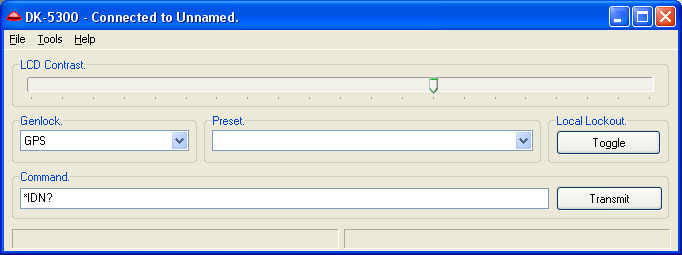
\includegraphics[width=1\textwidth]{fig/DK5300_MainWindow}
\caption{The DK-5300 main window.\label{fig:DK5300MainWindow}}
\end{figure}

The configuration of the PT5300 network settings are done using the NetFinder protocol. This enables you to configure the IP address, User name, Password, etc... on multiple PT5300's from one single location. The network port for the NetFinder protocol is 3040 (UDP).

The normal remote commands described in section \ref{cha:Remote} are transmitted using the Telnet protocol. The default port for Telnet is 23 (TCP).\\
\PasswordWarning
\newpage
\subsection{Connect to the PT5300.}
\label{cha:DK5300Connect}
\textbf{Operation:}

\begin{itemize}
\item Start the DK-5300.EXE and allow the program to connect to the network.
	\begin{itemize}
		\item The NetFinder protocol uses port 3040.
		\item The Telnet port can be changed but as default Telnet uses port 23.
	\end{itemize}
\item When the main window of DK-5300 is visible, go to the menu ``File'' and select ``NetFinder''.
\item When the NetFinder window is visible, click ``Refresh Instrument List''.

\begin{figure}[hbt]
\centering
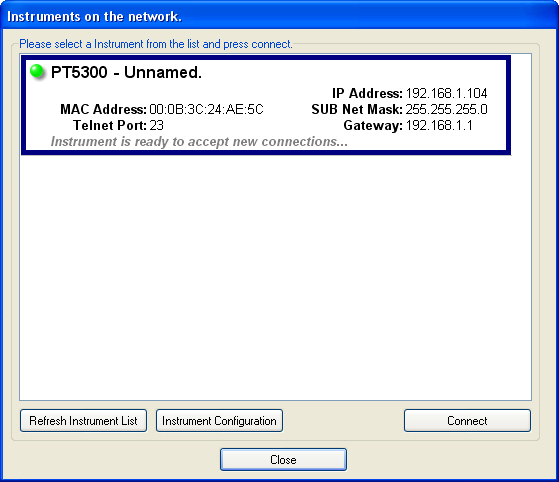
\includegraphics[width=0.6\textwidth]{fig/NetFinder_Search}
\caption{The NetFinder Window.\label{fig:NetFinderWindow}}
\end{figure}

	\begin{itemize}
		\item DK-5300 will now search the LAN for PT5300's. This process takes 10 seconds.
		\item During the search, PT5300's will be added to the list in the NetFinder window. Instruments are added in the order they are discovered.
		\item It is possible to connect to a PT5300 while the search is in progress.
%		\item From the NetFinder window it is also possible to change network settings for a PT5300.
		\item Each item in the instrument list will show the instrument type, the user configurable NetFinder name, the connection status of the instrument and optionally the IP settings of the instrument and Telnet port.\\\\
		\textbf{Connection status.}\\
					\raisebox{-0.5ex}{
\includegraphics{fig/Bubble_Green_Shadow}} - The Instrument is ready to accept new connections.\\
					\raisebox{-0.5ex}{
\includegraphics{fig/Bubble_Yellow_Shadow}} - The Instrument is busy. A connection has been established from another computer.\\
					\raisebox{-0.5ex}{
\includegraphics{fig/Bubble_Red_Shadow}} - Login in progress. A connection is being established from another computer.\\
					\raisebox{-0.5ex}{
\includegraphics{fig/Bubble_Grey_Shadow}} - Instrument is unavailable. The Telnet protocol has been disabled locally on the PT5300.\\
					\textit{	Please see section \ref{cha:NETWORK} for information about how to enable or disable the Telnet protocol.}
	\end{itemize}
\item Select from the instrument list the PT5300 you wish to connect to and press ``Connect''.
	\begin{itemize}
		\item You will be asked for the user name and password.
		\item The default user name is \textbf{\DefaultUser}. (Case sensitive.)
		\item The default password is \textbf{\DefaultPass}. (Case sensitive.)
		\item If ``Remember Login'' is checked the user name and password is saved in the DK-5300 configuration file.

		\begin{figure}[hbt]
		\centering
		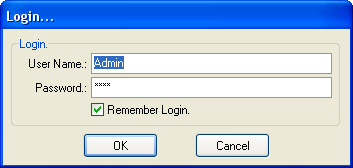
\includegraphics[width=0.3\textwidth]{fig/Login}
		\caption{The Login dialog.\label{fig:LoginDialog}}
		\end{figure}

	\end{itemize}
\item When a connection with a PT5300 has been established, the main window will then show basic options for remote control. \textit{(Figure \ref{fig:DK5300MainWindow}).}
	\begin{itemize}
		\item \textbf{LCD Contrast:} Set the LCD contrast.
		\item \textbf{Genlock:} Select the genlock source.
		\item \textbf{Preset:} Select the active preset. The dropdown box will show the active preset. If no preset is active the dropdown box will be empty.
		\item \textbf{Local Lockout:} Toggle whether or not the PT5300 responds to the local user interface.
		\item \textbf{Command:} Enter a command and press ``Transmit'' to send a specific command to the PT5300. Please see section \ref{cha:CommandRef} for further information about valid commands. There will be no indication whether or not the command has been executed unless the command is a query command.
	\end{itemize}
\end{itemize}

\subsection{Change network configuration.}
\label{cha:DK5300Configuration}

\textbf{Operation:}

\begin{itemize}
\item Open the NetFinder window.
	\begin{itemize}
		\item From the main window select ``File'' -> ``NetFinder''.
	\end{itemize}
\item When the NetFinder window is visible, click ``Refresh Instrument List''. \textit{(Figure \ref{fig:NetFinderWindow}).}
\item Select from the instrument list the PT5300 you wish to configure and press ``Instrument Configuration''.
\item The Instrument Configuration window will appear.

\begin{figure}[hbt]
\centering
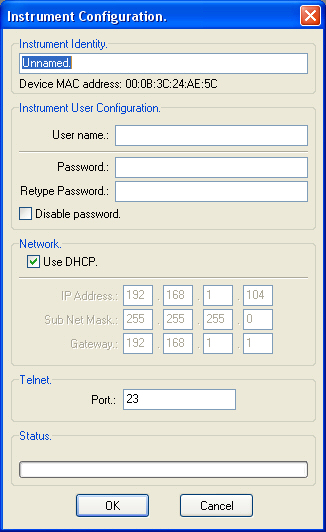
\includegraphics[width=0.28\textwidth]{fig/NetFinder_Config}
\caption{The Instrument Configuration Window.\label{fig:NetFinderConfigWindow}}
\end{figure}
\item	\textbf{Configuration options.}\\
	\begin{itemize}
		\item \textbf{Instrument Identity:}\\The text field allows you to change the NetFinder name. When multiple PT5300's are connected to the LAN the NetFinder name is used for easy identification in the Instrument List \textit{(Figure: \ref{fig:NetFinderWindow})}.\\The NetFinder name is also shown in the main window of DK-5300 when a connection with the instrument has been established.
		\item \textbf{Instrument User Configuration:}\\The text field ``User Name'' allows you to change the default user name. If this field is left blank no changes will be made to the user name.\\The password fields allows you to change the default password. The two password fields must match each other. The password can be disabled by checking ``Disable Password''. If the password fields are left blank, no changes will be made to the password.
		\item \textbf{Network.}\\The instrument is by default configured to use DHCP. This can be disabled by un-checking DHCP. When DHCP is disabled the text fields for IP configuration is enabled. If you enter the wrong IP settings you might not be able to reconnect to the instrument.\\\\\textbf{The DHCP and IP settings can always be reconfigured locally on the instrument. Please see section \ref{cha:NETWORK} for further information about how to do this.}
		\item \textbf{Telnet:}\\The default Telnet port is 23. In the Telnet field this can be changed. The Telnet port can be configured to a value between 1 and 65535.
	\end{itemize}
\item Click ``OK'' to apply the changes. If ``Cancel'' is selected the changes will be discarded.
	\begin{itemize}
		\item When you apply the changes you will be asked for the user name and password. \textit{(Figure \ref{fig:LoginDialog}).}
		\item The default user name is \textbf{\DefaultUser}. (Case sensitive.)
		\item The default password is \textbf{\DefaultPass}. (Case sensitive.)
		\item If ``Remember Login'' is checked the user name and password is saved in the DK-5300 configuration file.
		\item A message box will then appear stating whether or not the changes have been accepted by the instrument.
		\item When the configuration has been changed you should wait approximately 30 seconds for the changes to take effect and then refresh the instrument list.
	\end{itemize}
\end{itemize}
The instrument can not be reconfigured using the NetFinder protocol while a Telnet connection is active.\\If the network settings are changed locally on the instrument (please see section \ref{cha:NETWORK} for further information) all connections will be disconnected while reloading the new configuration.
\newpage
\subsection{DK-5300 Options}
\textbf{Operation:}

\begin{itemize}
\item Open the option window.
	\begin{itemize}
		\item From the main window select ``Tools'' -> ``Options...''.
	\end{itemize}
\item The option window currently have two options.

\begin{figure}[hbt]
\centering
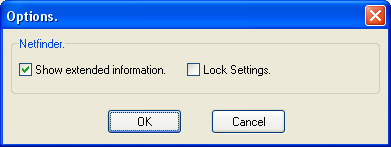
\includegraphics[width=0.35\textwidth]{fig/DK5300_Options}
\caption{The DK-5300 Option Window.\label{fig:DK5300OptionWindow}}
\end{figure}
	\begin{itemize}
		\item \textbf{Show extended information:}\\When checked, the instrument list in the NetFinder window will show the MAC address, Telnet Port and IP information for every instrument discovered on the LAN. If un-checked, only the NetFinder name and connection status is shown. \textit{(Figure: \ref{fig:NetFinderWindow})}
		\item \textbf{Lock Settings:}\\When checked, the ``Instrument Configuration'' function in the NetFinder window will be disabled.
	\end{itemize}
\item Click ``OK'' to apply the changes. If ``Cancel'' is selected the changes will be discarded.
\end{itemize}

\clearpage

\clearpage
\end{document}

